\documentclass[12pt]{book}
\usepackage[margin=1in]{geometry}
\usepackage{fontspec}
\usepackage{graphicx}
\usepackage[english]{babel} 
%\setmainfont[Script=Devanagari]{Lohit Devanagari}
\newfontfamily\sanskrit[Script=Devanagari]{Lohit Devanagari}
\usepackage{tocloft}
\renewcommand{\cftchapdotsep}{\cftdotsep}
\usepackage{hyperref}

\usepackage{fancyhdr}
\pagestyle{fancy}
%\fancyhead{} % clear all header fields
\renewcommand{\headrulewidth}{0pt} % no line in header area
\fancyhead[LE,RO]{\sanskrit गीतोच्चारण}
\fancyfoot{} % clear all footer fields
\fancyfoot[LE,RO]{\thepage}           % page number in "outer" position of footer line
\fancyfoot[RE,LO]{\tiny \bf Copyrighted Material, All Rights Reserved} % other info in "inner" position of footer line


\usepackage{eso-pic}
\AddToShipoutPictureBG*{%
	\AtTextLowerLeft{\makebox[\textwidth][r]{%
			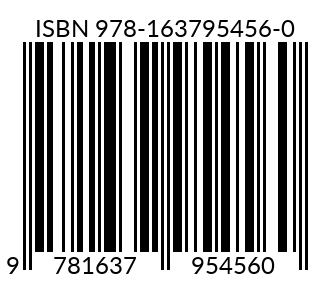
\includegraphics[keepaspectratio]{ISBN}}}}

\begin{document}
\title{
	
\includegraphics[scale=0.2,keepaspectratio]{eps5black}\\
	\sanskrit गीतोच्चारण}
\author{\sanskrit विश्वजीत अग्रवाल}
\date{January 2021	}
\maketitle
\begin{quotation}
	\begin{center}\sanskrit
	यदा यदा हि धर्मस्य ग्लानिर्भवति भारत  । 
	
	अभ्युत्थानमधर्मस्य तदाऽऽत्मानं सृजाम्यहम्  ॥ 
\end{center}
\end{quotation}
\begin{center}
	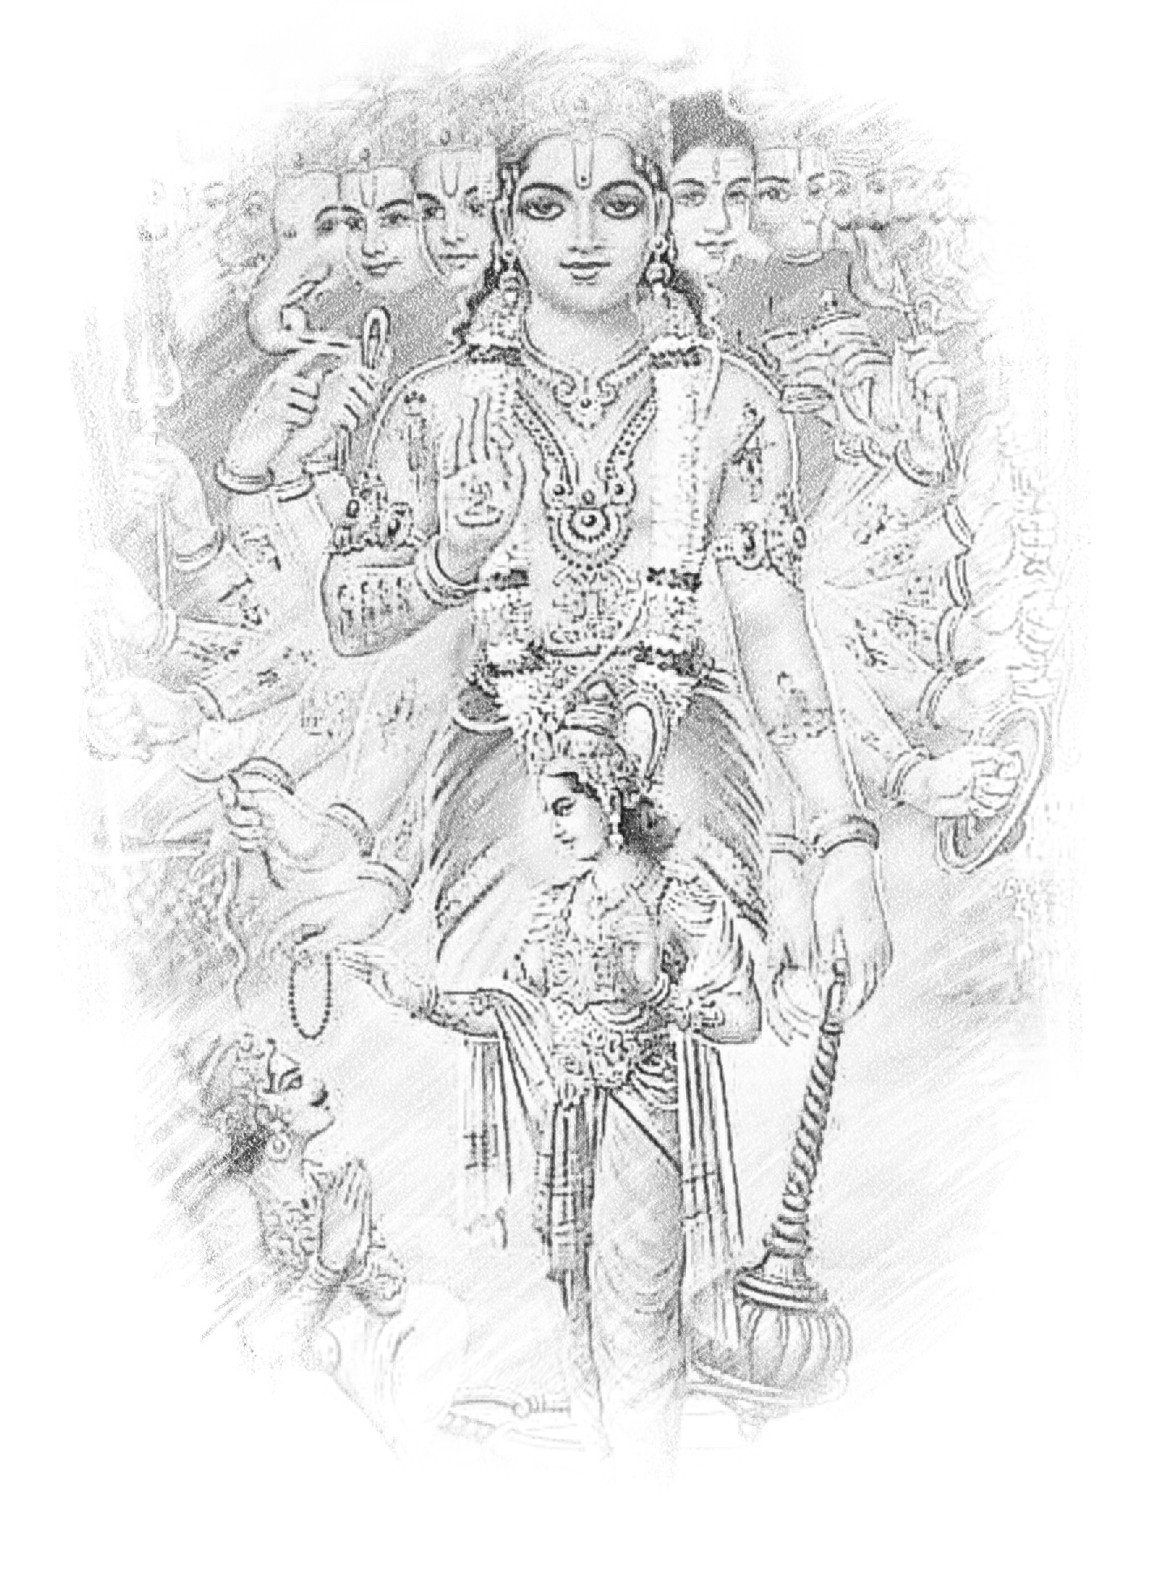
\includegraphics[scale=0.35,keepaspectratio]{CoverImage.jpg}
\end{center}
\chapter*{}
\begin{center}
	
\includegraphics[scale=0.25,keepaspectratio]{eps2}
\end{center}
\chapter*{\sanskrit प्राक्कथन}
\sanskrit

गीता एक अद्भुत पुस्तक है ।  गीता की महत्ता बहुत लम्बे समय से ज्ञात है, इसीलिए गीता का अनुवाद अनेक भाषाओं में हुआ है, परंतु गीता का मूल स्वरुप संस्कृत में है ।  गीता को संस्कृत लिखने से जुडी हुई एक रोचक कथा में यह बताया गया है, कि गीता के लिखने के लिए व्यास ऋषि ने श्री गणेशजी को आमंत्रण दिया ।  लेकिन अपने चंचल स्वभाव के कारणवश गणेशजी ने गीता को लिखने के पहले व्यासजी एक समक्ष यह शर्त रखी व्यासजी को उन्हें लगातार व्यस्त रखना होगा अन्यथा वह ऊबकर चले जायेंगे ।  इसके प्रत्युत्तर में व्यासजी ने भी अपनी एक शर्त रखी कि गणेश कुछ भी समझे बिना न लिखें ।  गणेशजी अपनी तीव्र बुद्धि से व्यासजी का गीतोच्चारण बहुत जल्दी समझकर तुरंत लिख लेते थे, इस पर व्यासजी को श्वांस लेने तक की कठिनाई आने लगी ।  तब  उन्होंने गीता के श्लोको को बीच-बीच में अत्यधिक मुश्किल बनाना आरम्भ कर दिया, जिससे गणेशजी को समझने में थोड़ा समय लगने लगा और व्यासजी को श्वांस लेने का अवकाश मिलने लगा ।  इस प्रकार व्यासजी की इमला और गणेशजी की लिखावट से गीता लिखने का कार्य सम्पूर्ण हुआ ।  लेकिन गीता के श्लोक थोड़े कठिन हो गए ।  उदाहरण स्वरुप पांचवे अध्याय के आठवें श्लोक की दूसरी पंक्ति को पढ़ने की कोशिश कीजिये । 

\begin{quotation}\sanskrit
नैव किंचित्करोमीति युक्तो मन्येत तत्ववित्‌  । 

पश्यञ्श्रण्वन्स्पृशञ्जिघ्रन्नश्नन्गच्छन्स्वपन्श्वसन्‌  ॥ ५.८ ॥  
\end{quotation}
जब गीता का अनुवाद अन्य भाषाओँ में हुआ तब ऐसे श्लोकों को संधि-विच्छेद करने के बाद ही लिखा गया, इस कारण अन्य भाषाओं में गीता पड़ना आसान है ।  परन्तु संस्कृत में लिखी गयी गीता आज भी कठिन ही है ।  प्रस्तुत पुस्तक में यह प्रयास किया गया है, देवनागरी भाषा में ही गीता के श्लोकों को संधि-विच्छेद करके लिखा जाए । 

\begin{quotation}\sanskrit
नैव किंचित करोमीति, युक्तो मन्येत तत्व वित्‌  । 

पश्यन् श्रण्वन् स्पर्शन् जिघ्रन्न, अस्नन् गच्छन् स्वपन् श्वसन्‌  ॥ ५.८ ॥ 
\end{quotation}
गीता को समझने के लिए कहा जाता है कि कई जन्म लेने पड़ते हैं ।  लेकिन इसका आरम्भ उचित उच्चारण से ही हो तो अच्छा है ।  संधि-विच्छेद के पश्चात आधे से ज्यादा श्लोक देवनागरी पढ़ने वालों को समझ में भी आ सकता है ।  यदि आपको कोई त्रुटि मिले तो कृपया अवश्य बतायें । 
इस पुस्तक के संकलन के लिये मूल श्लोक \textrm{IIT} कानपुर की \textrm{website} से लिये गये हैं ।  \textrm{https://www.gitasupersite.iitk.ac.in}

\begin{quotation}
जय श्री कृष्ण

विश्वजीत अग्रवाल 

\textrm{Vishv.Jeet@gmail.com}

\textrm{January 2021}
\end{quotation}
\AddToShipoutPictureBG*{%
	\AtTextLowerLeft{\makebox[\textwidth][r]{%
			
\includegraphics[scale=0.05,keepaspectratio]{eps4}}}}
\tableofcontents
\chapter{\sanskrit{अर्जुनविषादयोग}}
\sanskrit

\paragraph{\sanskrit धृतराष्ट्र उवाच}

\begin{quotation}
	धर्मक्षेत्रे कुरुक्षेत्रे समवेता युयुत्सवः  । 
	
	मामकाः पाण्डवाश्चैव किमकुर्वत संजय  ॥ १.१ ॥  मूल श्लोक

\end{quotation}

\begin{quotation}
धर्म-क्षेत्रे कुरु-क्षेत्रे, समवेता युयुत्सवः  । 

मामकाः पाण्डवाश् चैव, किम अकुर्वत संजय   ॥ १.१ ॥   उच्चारण

\noindent\rule{16cm}{0.4pt} 
\end{quotation}

\paragraph{\sanskrit सञ्जय उवाच}

\begin{quotation}
दृष्टवा तु पाण्डवानीकं व्यूढं दुर्योधनस्तदा  । 

आचार्यमुपसंगम्य राजा वचनमब्रवीत्‌  ॥ १.२ ॥  मूल श्लोक
\end{quotation}

\begin{quotation}

दृष्ट्वा तु पाण्डवा-अनीकं, व्यूढं दुर्योधनस् तदा  । 

आचार्यम उप-संगम्य, राजा वचनम् अब्रवीत्  ॥ १.२ ॥  उच्चारण

\noindent\rule{16cm}{0.4pt} 
\end{quotation}


\begin{quotation} 

पश्यैतां पाण्डुपुत्राणामाचार्य महतीं चमूम्‌  । 

व्यूढां द्रुपदपुत्रेण तव शिष्येण धीमता  ॥ १.३ ॥  मूल श्लोक
\end{quotation}

\begin{quotation} 

पश्यैतां पाण्डु पुत्राणाम्, आचार्य महतीं चमूम  ।  

व्यूढां द्रुपद पुत्रेण, तव शिष्येण धीमता  ॥ १.३ ॥  उच्चारण

\noindent\rule{16cm}{0.4pt} 
\end{quotation}


\begin{quotation} 

अत्र शूरा महेष्वासा भीमार्जुनसमा युधि  ।  

युयुधानो विराटश्च द्रुपदश्च महारथः  ॥ १.४ ॥  मूल श्लोक
\end{quotation}

\begin{quotation}

अत्र शूरा महेष्वासा, भीमार्जुन-समा युधि  ।  

युयुधानो विराटश् च, द्रुपदश् च महारथः  ॥ १.४ ॥  उच्चारण

\noindent\rule{16cm}{0.4pt} 
\end{quotation}


\begin{quotation} 


धृष्टकेतुश्चेकितानः काशिराजश्च वीर्यवान्‌  ।  

पुरुजित्कुन्तिभोजश्च शैब्यश्च नरपुङवः  ॥ १.५ ॥  मूल श्लोक
\end{quotation}

\begin{quotation}

धृष्ट-केतुश चेकितानः, काशि-राजश् च वीर्यवान्  ।  

पुरुजित कुन्ति भोजश् च, शैब्यश्  च नर नरपुङवः  ॥ १.५ ॥  उच्चारण

\noindent\rule{16cm}{0.4pt} 
\end{quotation}


\begin{quotation} 

युधामन्युश्च विक्रान्त उत्तमौजाश्च वीर्यवान्‌  ।  

सौभद्रो द्रौपदेयाश्च सर्व एव महारथाः  ॥ १.६ ॥  मूल श्लोक
\end{quotation}

\begin{quotation}

युधामन्युश् च विक्रान्त, उत्तमौजाश् च वीर्यवान्  ।  

सौभद्रो द्रौपदेयाश् च, सर्व एव महारथाः  ॥ १.६ ॥  उच्चारण

\noindent\rule{16cm}{0.4pt} 
\end{quotation}


\begin{quotation} 

अस्माकं तु विशिष्टा ये तान्निबोध द्विजोत्तम  ।  

नायका मम सैन्यस्य सञ्ज्ञार्थं तान्ब्रवीमि ते  ॥ १.७ ॥  मूल श्लोक
\end{quotation}

\begin{quotation}

अस्माकं तु विशिष्टा ये, तान निबोध द्विजोत्तम  ।  

नायका मम सैन्यस्य, संज्ञार्थं तान ब्रवीमि ते  ॥ १.७ ॥  उच्चारण

\noindent\rule{16cm}{0.4pt} 
\end{quotation}


\begin{quotation} 

भवान्भीष्मश्च कर्णश्च कृपश्च समितिञ्जयः  ।  

अश्वत्थामा विकर्णश्च सौमदत्तिस्तथैव च  ॥ १.८ ॥  मूल श्लोक
\end{quotation}

\begin{quotation}

भवान् भीष्मश् च कर्णश् च, कृपश् च समितिञ् जयः ।  

अश्वत्थामा विकर्णश् च, सौमदत्तिस् तथैव च  ॥ १.८ ॥  उच्चारण

\noindent\rule{16cm}{0.4pt} 
\end{quotation}


\begin{quotation} 

अन्ये च बहवः शूरा मदर्थे त्यक्तजीविताः  ।  

नानाशस्त्रप्रहरणाः सर्वे युद्धविशारदाः  ॥ १.९ ॥  मूल श्लोक
\end{quotation}

\begin{quotation}

अन्ये च बहवः शूरा, मदर्थे त्यक्त जीविताः  ।  

नाना शस्त्र प्रहरणाः, सर्वे युद्ध विशारदाः  ॥ १.९ ॥  उच्चारण

\noindent\rule{16cm}{0.4pt} 
\end{quotation}


\begin{quotation} 

अपर्याप्तं तदस्माकं बलं भीष्माभिरक्षितम्‌  ।  

पर्याप्तं त्विदमेतेषां बलं भीमाभिरक्षितम्‌  ॥ १.१० ॥  मूल श्लोक
\end{quotation}

\begin{quotation}

अपर्याप्तं तद अस्माकं, बलं भीष्मा भिरक्षितम्  ।  

पर्याप्तं त्व इदम इतेषां, बलं भीमा भिरक्षितम्  ॥ १.१० ॥  उच्चारण

\noindent\rule{16cm}{0.4pt} 
\end{quotation}


\begin{quotation} 
अयनेषु च सर्वेषु यथाभागमवस्थिताः  ।  

भीष्ममेवाभिरक्षन्तु भवन्तः सर्व एव हि  ॥ १.११ ॥  मूल श्लोक
\end{quotation}

\begin{quotation}

अयनेषु च सर्वेषु, यथा भागम अवस्थिताः  ।  

भीष्मम् एवा भिरक्षन्तु, भवन्तः सर्व एव हि  ॥ १.११ ॥  उच्चारण

\noindent\rule{16cm}{0.4pt} 
\end{quotation}


\begin{quotation} 

तस्य सञ्जनयन्हर्षं कुरुवृद्धः पितामहः  ।  

सिंहनादं विनद्योच्चैः शङ्खं दध्मो प्रतापवान्‌   ॥ १.१२ ॥  मूल श्लोक
\end{quotation}

\begin{quotation}

तस्य संजनयन् हर्षं, कुरु वृद्धः पितामहः  ।  

सिंहनादं विनद्योच्चैः, शङ्खं दध्मौ प्रतापवान्  ॥ १.१२ ॥  उच्चारण

\noindent\rule{16cm}{0.4pt} 
\end{quotation}


\begin{quotation} 

ततः शंखाश्च भेर्यश्च पणवानकगोमुखाः  ।  

सहसैवाभ्यहन्यन्त स शब्दस्तुमुलोऽभवत्‌  ॥ १.१३ ॥  मूल श्लोक
\end{quotation}

\begin{quotation}

ततः शङ्खाश् च भेर्यश् च, पण-वानक गोमुखाः  ।  

सहसा एवा अभय-अन्यन्त, स शब्दस तूमुलोऽ अभवत्  ॥ १.१३ ॥  उच्चारण

\noindent\rule{16cm}{0.4pt} 
\end{quotation}


\begin{quotation} 

ततः श्वेतैर्हयैर्युक्ते महति स्यन्दने स्थितौ  ।  

माधवः पाण्डवश्चैव दिव्यौ शंखौ प्रदध्मतुः   ॥ १.१४ ॥  मूल श्लोक
\end{quotation}

\begin{quotation}

ततः श्वेतैर् हयैर् युक्ते, महति स्यन्दने स्थितौ  ।  

माधवः पाण्डवश् च एैव, दिव्यौ शङ्खौ प्रदध्-मतुः  ॥ १.१४ ॥  उच्चारण

\noindent\rule{16cm}{0.4pt} 
\end{quotation}


\begin{quotation} 

पाञ्चजन्यं हृषीकेशो देवदत्तं धनञ्जयः  ।  

पौण्ड्रं दध्मौ महाशंख भीमकर्मा वृकोदरः  ॥ १.१५ ॥  मूल श्लोक
\end{quotation}

\begin{quotation}

पाञ्चजन्यं हृषीकेशो, देवदत्तं धनंजयः  ।  

पौण्ड्रं दध्मौ महाशङ्खं, भीम कर्मा वृकोदरः  ॥ १.१५ ॥  उच्चारण

\noindent\rule{16cm}{0.4pt} 
\end{quotation}


\begin{quotation} 

अनन्तविजयं राजा कुन्तीपुत्रो युधिष्ठिरः  ।  

नकुलः सहदेवश्च सुघोषमणिपुष्पकौ ।  
  ॥ १.१६ ॥  मूल श्लोक
\end{quotation}

\begin{quotation}

अनन्त विजयं राजा, कुन्ती पुत्रो युधिष्ठिरः  ।  

नकुलः सहदेवश् च, सुघोष मणि पुष्पकौ  ॥ १.१६ ॥  उच्चारण

\noindent\rule{16cm}{0.4pt} 
\end{quotation}


\begin{quotation} 
काश्यश्च परमेष्वासः शिखण्डी च महारथः  ।  

धृष्टद्युम्नो विराटश्च सात्यकिश्चापराजितः  ॥ १.१७ ॥  मूल श्लोक
\end{quotation}

\begin{quotation}

काश्यश् च परमेष्वासः, शिखण्डी च महारथः  ।  

धृष्ट-द्युम्-नो विराटश् च, सात्यकिश् च पराजितः  ॥ १.१७ ॥  उच्चारण

\noindent\rule{16cm}{0.4pt} 
\end{quotation}


\begin{quotation} 

द्रुपदो द्रौपदेयाश्च सर्वशः पृथिवीपते  ।  

सौभद्रश्च महाबाहुः शंखान्दध्मुः पृथक्पृथक्‌  ॥ १.१८ ॥  मूल श्लोक
\end{quotation}

\begin{quotation}

द्रुपदो द्रौपदेयाश् च, सर्वशः पृथिवीपते  ।  

सौभद्रश् च महाबाहुः, शङ्खान् दध्मुः पृथक्-पृथक्  ॥ १.१८ ॥  उच्चारण

\noindent\rule{16cm}{0.4pt} 
\end{quotation}


\begin{quotation} 

स घोषो धार्तराष्ट्राणां हृदयानि व्यदारयत्‌  ।  

नभश्च पृथिवीं चैव तुमुलो व्यनुनादयन्‌  ॥ १.१९ ॥  मूल श्लोक
\end{quotation}

\begin{quotation}

स घोषो धार्त-राष्ट्राणां, हृदयानि व्यदार-यत्  ।  

नभश् च पृथिवीं च एैव, तुमुलो भयनु नादयन्  ॥ १.१९ ॥  उच्चारण

\noindent\rule{16cm}{0.4pt} 
\end{quotation}


\begin{quotation} 

अथ व्यवस्थितान्दृष्ट्वा धार्तराष्ट्रान्‌ कपिध्वजः  ।  

प्रवृत्ते शस्त्रसम्पाते धनुरुद्यम्य पाण्डवः  ।  
 
हृषीकेशं तदा वाक्यमिदमाह महीपते   ॥ १.२० ॥  मूल श्लोक
\end{quotation}

\begin{quotation}

अथ व्यवस्थितान् दृष्ट्वा, धार्त-राष्ट्रान् कपिध्वजः ।  

प्रवृत्ते शस्त्र सम्पाते, धनुर उद्यम्य पाण्डवः  ।  

हृषीकेशं तदा वाक्यम,  इदम अहा महीपते  ॥ १.२० ॥  उच्चारण

\noindent\rule{16cm}{0.4pt} 
\end{quotation}

\paragraph{\sanskrit अर्जुन उवाच}

\begin{quotation} 



सेनयोरुभयोर्मध्ये रथं स्थापय मेऽच्युत  ।  

यावदेतान्निरीक्षेऽहं योद्धुकामानवस्थितान्‌  ॥ १.२१ ॥ 

कैर्मया सह योद्धव्यमस्मिन् रणसमुद्यमे  ॥ १.२२ ॥  मूल श्लोक
\end{quotation}

\begin{quotation}

सेनयोर उभयोर मध्ये, रथं स्थापय मेऽ अच्युत  ।  

यावद इतान् निरीक्षेऽ अहं, योद्धु कामान् अवस्थितान्  ॥ १.२१ ॥ 

कैर्मया सह योद्ध-व्यम, अस्मिन् रण समुद्यमे  ॥ १.२२ ॥  उच्चारण

\noindent\rule{16cm}{0.4pt} 
\end{quotation}


\begin{quotation} 

योत्स्यमानानवेक्षेऽहं य एतेऽत्र समागताः  ।  

धार्तराष्ट्रस्य दुर्बुद्धेर्युद्धे प्रियचिकीर्षवः  ॥ १.२३ ॥  मूल श्लोक
\end{quotation}

\begin{quotation}

योत्स्य मानान् अवेक्षेऽ अहं, य एतेऽ अत्र समागताः  ।  

धार्त-राष्ट्रस्य दुर्बुद्धेर, युद्ध प्रिये चिकीर्षवः  ॥ १.२३ ॥  उच्चारण

\noindent\rule{16cm}{0.4pt} 
\end{quotation}


\paragraph{\sanskrit सञ्जय उवाच}
\begin{quotation} 


एवमुक्तो हृषीकेशो गुडाकेशेन भारत  ।  

सेनयोरुभयोर्मध्ये स्थापयित्वा रथोत्तमम्‌  ॥ १.२४ ॥  मूल श्लोक
\end{quotation}

\begin{quotation}

एवम उक्तो हृषीकेशो, गुडाकेशेन भारत  ।  

सेनयोर उभयोर मध्ये, स्थापयित्वा रथ-उत्तमम्  ॥ १.२४ ॥  उच्चारण

\noindent\rule{16cm}{0.4pt} 
\end{quotation}


\begin{quotation} 

भीष्मद्रोणप्रमुखतः सर्वेषां च महीक्षिताम्‌  ।  

उवाच पार्थ पश्यैतान्‌ समवेतान्‌ कुरूनिति  ॥ १.२५ ॥  मूल श्लोक
\end{quotation}

\begin{quotation}

भीष्म द्रोण प्रमुखतः, सर्वेषां च महीक्षिताम्  ।  

उवाच पार्थ पश्यैतान्, समवेतान् कुरून् इति  ॥ १.२५ ॥  उच्चारण

\noindent\rule{16cm}{0.4pt} 
\end{quotation}


\begin{quotation} 

तत्रापश्यत्स्थितान्‌ पार्थः पितृनथ पितामहान्‌  ।  

आचार्यान्मातुलान्भ्रातृन्पुत्रान्पौत्रान्सखींस्तथा  ।  

श्वशुरान्‌ सुहृदश्चैव सेनयोरुभयोरपि  ॥ १.२६ - १.२७ ॥  मूल श्लोक
\end{quotation}

\begin{quotation}

तत्रा पश्यत स्थितान् पार्थः, पितृ़न् अथ पितामहान्  ।  

आचार्यान् मातुलान् भ्रातेन्, पुत्रान् पौत्रान् सखींस तथा  । 

श्वशुरान् सुहृदश च एैव, सेनयोर उभयोर अपि  ॥ १.२६ - १.२७ ॥  उच्चारण

\noindent\rule{16cm}{0.4pt} 
\end{quotation}


\begin{quotation} 


तान्समीक्ष्य स कौन्तेयः सर्वान्‌ बन्धूनवस्थितान्‌  ।  
 
कृपया परयाविष्टो विषीदत्रिदमब्रवीत्‌  ॥ १.२७ - १.२८ ॥  मूल श्लोक
\end{quotation}

\begin{quotation}

तान समीक्ष्य स कौन्तेयः, सर्वान् बन्धून अवस्थितान्  ।  

कृपया परयाविष्टो, विषीदन्न इदं अब्रवीत्  ॥ १.२७ - १.२८ ॥  उच्चारण

\noindent\rule{16cm}{0.4pt} 
\end{quotation}

\paragraph{\sanskrit अर्जुन उवाच}

\begin{quotation} 


दृष्टेवमं स्वजनं कृष्ण युयुत्सुं समुपस्थितम्‌  ।  

सीदन्ति मम गात्राणि मुखं च परिशुष्यति  । 
 
वेपथुश्च शरीरे में रोमहर्षश्च जायते  ॥ १.२८ - १.२९ ॥  मूल श्लोक
\end{quotation}

\begin{quotation}

दृष्ट्वेमं स्वजनं कृष्ण, युयुत्सुं सम-उपस्थितम्  ।  

सीदन्ति मम गात्राणि, मुखं च परिश उष्यति  । 

वेपथुश् च शरीरे में, रोमहर्षश् च जायते  ॥ १.२८ - १.२९ ॥  उच्चारण

\noindent\rule{16cm}{0.4pt} 
\end{quotation}


\begin{quotation} 

गाण्डीवं स्रंसते हस्तात्त्वक्चैव परिदह्यते  ।  
 
न च शक्नोम्यवस्थातुं भ्रमतीव च मे मनः  ॥ १.३० ॥  मूल श्लोक
\end{quotation}

\begin{quotation} 

गाण्डीवं स्रंसते हस्तात्, त्वक च एैव परिदह्यते  ।  

न च शक्नोम्य अवस्थातुं, भ्रमतीव च मे मनः  ॥ १.३० ॥  उच्चारण

\noindent\rule{16cm}{0.4pt} 
\end{quotation}


\begin{quotation} 

निमित्तानि च पश्यामि विपरीतानि केशव  ।  
 
न च श्रेयोऽनुपश्यामि हत्वा स्वजनमाहवे  ॥ १.३१ ॥  मूल श्लोक
\end{quotation}

\begin{quotation}

निमित्तानि च पश्यामि, विपरीतानि केशव  ।  
 
न च श्रेयोऽ अनु-पश्यामि, हत्वा स्वजनम आहवे  ॥ १.३१ ॥  उच्चारण

\noindent\rule{16cm}{0.4pt} 
\end{quotation}


\begin{quotation} 

न काङ्‍क्षे विजयं कृष्ण न च राज्यं सुखानि च  ।  
 
किं नो राज्येन गोविंद किं भोगैर्जीवितेन वा  ॥ १.३२ ॥  मूल श्लोक
\end{quotation}

\begin{quotation}

न काङ्क्षे विजयं कृष्ण, न च राज्यं सुखानि च  ।  
 
किं नो राज्येन गोविन्द, किं भोगैर् जीवितेन वा  ॥ १.३२ ॥  उच्चारण

\noindent\rule{16cm}{0.4pt} 
\end{quotation}


\begin{quotation} 

येषामर्थे काङक्षितं नो राज्यं भोगाः सुखानि च  ।  

त इमेऽवस्थिता युद्धे प्राणांस्त्यक्त्वा धनानि च  ॥ १.३३ ॥  मूल श्लोक
\end{quotation}

\begin{quotation}

येषाम अर्थे काङ्क्षितं नो, राज्यं भोगाः सुखानि च  ।  

त इमेऽ अवस्थिता युद्धे, प्राणांस्य त्यक्त्वा धनानि च  ॥ १.३३ ॥  उच्चारण

\noindent\rule{16cm}{0.4pt} 
\end{quotation}


\begin{quotation} 

आचार्याः पितरः पुत्रास्तथैव च पितामहाः  ।  
 
मातुलाः श्वशुराः पौत्राः श्यालाः संबंधिनस्तथा  ॥ १.३४ ॥  मूल श्लोक
\end{quotation}

\begin{quotation}

आचार्याः पितरः पुत्रास, तथैव च पितामहाः ।  

मातुलाः च श्रशुराः पौत्राः श्यालाः सम्बन्धिनस तथा  ॥ १.३४ ॥  उच्चारण

\noindent\rule{16cm}{0.4pt} 
\end{quotation}


\begin{quotation} 

एतान्न हन्तुमिच्छामि घ्नतोऽपि मधुसूदन  ।  
 
अपि त्रैलोक्यराज्यस्य हेतोः किं नु महीकृते  ॥ १.३५ ॥  मूल श्लोक
\end{quotation}

\begin{quotation}

एतान् न हन्तुम इच्छामि, घ्नतोऽ अपि मधुसूदन ।  

अपि त्रैलोक्य राज्यस्य हेतोः, किं नु महीकृते  ॥ १.३५ ॥   उच्चारण

\noindent\rule{16cm}{0.4pt} 
\end{quotation}


\begin{quotation} 

निहत्य धार्तराष्ट्रान्न का प्रीतिः स्याज्जनार्दन  ।  


पापमेवाश्रयेदस्मान्‌ हत्वैतानाततायिनः  ॥ १.३६ ॥  मूल श्लोक
\end{quotation}

\begin{quotation}

निहत्य धार्तराष्ट्रान् नः, का प्रीतिः स्याज् जनार्दन ।  


पापम एव आश्रयेद अस्मां, हत्वैतान आततायिनः  ॥ १.३६ ॥  उच्चारण

\noindent\rule{16cm}{0.4pt} 
\end{quotation}


\begin{quotation} 

तस्मान्नार्हा वयं हन्तुं धार्तराष्ट्रान्स्वबान्धवान्‌  ।  
 

स्वजनं हि कथं हत्वा सुखिनः स्याम माधव  ॥ १.३७ ॥  मूल श्लोक
\end{quotation}

\begin{quotation}

तस्मान् नर्हा वयं हन्तुं, धार्त-राष्ट्रान् स बान्धवान्  ।  


स्वजनं हि कथं हत्वा, सुखिनः स्याम माधव  ॥ १.३७ ॥  उच्चारण

\noindent\rule{16cm}{0.4pt}
\end{quotation}


\begin{quotation}
यद्यप्येते न पश्यन्ति लोभोपहतचेतसः  ।  

कुलक्षयकृतं दोषं मित्रद्रोहे च पातकम्‌  ॥ १.३८ ॥  मूल श्लोक
\end{quotation}

\begin{quotation}

यद्य अप्य एते न पश्यन्ति, लोभो-पहत चेतसः  ।  


कुलक्षय कृतं दोषं, मित्र-द्रोहे च पातकम्  ॥ १.३८ ॥  उच्चारण

\noindent\rule{16cm}{0.4pt} 
\end{quotation}


\begin{quotation} 
कथं न ज्ञेयमस्माभिः पापादस्मान्निवर्तितुम्‌  ।  


कुलक्षयकृतं दोषं प्रपश्यद्भिर्जनार्दन  ॥ १.३९ ॥  मूल श्लोक
\end{quotation}

\begin{quotation}

कथं न ज्ञेयम अस्माभिः, पापाद अस्मान नि-वर्तितुम्‌  ।  


कुलक्षय कृतं दोषं, प्रपश्य-यद्भिर जनार्दन  ॥ १.३९ ॥  उच्चारण

\noindent\rule{16cm}{0.4pt} 
\end{quotation}


\begin{quotation} 

कुलक्षये प्रणश्यन्ति कुलधर्माः सनातनाः  ।  


धर्मे नष्टे कुलं कृत्स्नमधर्मोऽभिभवत्युत  ॥ १.४० ॥  मूल श्लोक
\end{quotation}

\begin{quotation}

कुलक्षये प्रणश्यन्ति, कुलधर्माः सनातनाः  ।  


धर्मे नष्टे कुलं कृत्सनं, अधर्मोऽ अभि-भवत्य उत  ॥ १.४० ॥  उच्चारण

\noindent\rule{16cm}{0.4pt} 
\end{quotation}


\begin{quotation} 

अधर्माभिभवात्कृष्ण प्रदुष्यन्ति कुलस्त्रियः  ।  


स्त्रीषु दुष्टासु वार्ष्णेय जायते वर्णसंकरः  ॥ १.४१ ॥  मूल श्लोक
\end{quotation}

\begin{quotation}

अधर्मा अभि-भवात कृष्ण, प्रदुष्यन्ति कुल-स्त्रियः  ।  


स्त्रीषु दुष्टासु वार्ष्णेय, जायते वर्णसङ्करः  ॥ १.४१ ॥  उच्चारण

\noindent\rule{16cm}{0.4pt} 
\end{quotation}


\begin{quotation} 

संकरो नरकायैव कुलघ्नानां कुलस्य च  ।  


पतन्ति पितरो ह्येषां लुप्तपिण्डोदकक्रियाः  ॥ १.४२ ॥  मूल श्लोक
\end{quotation}

\begin{quotation}

संकरो नरकाय एैव, कुलघ्नानां कुलस्य च  ।  


पतन्ति पितरो ह्य एषां, लुप्त पिण्डोदक क्रियाः  ॥ १.४२ ॥  उच्चारण

\noindent\rule{16cm}{0.4pt} 
\end{quotation}


\begin{quotation} 

दोषैरेतैः कुलघ्नानां वर्णसंकरकारकैः  ।  


उत्साद्यन्ते जातिधर्माः कुलधर्माश्च शाश्वताः  ॥ १.४३ ॥  मूल श्लोक
\end{quotation}

\begin{quotation}

दोषैर एतैः कुलघ्नानां, वर्णसङ्कर कारकैः  ।  


उत्साद्-यन्ते जाति-धर्माः, कुल धर्माश् च शाश्वताः  ॥ १.४३ ॥  उच्चारण

\noindent\rule{16cm}{0.4pt} 
\end{quotation}


\begin{quotation} 

उत्सन्नकुलधर्माणां मनुष्याणां जनार्दन  ।  


नरकेऽनियतं वासो भवतीत्यनुशुश्रुम  ॥ १.४४ ॥  मूल श्लोक
\end{quotation}

\begin{quotation}

उत्सन्न कुल धर्माणां, मनुष्याणां जनार्दन  ।  


नरकेऽ नियतं वासो, भवतीत अनु-शु-श्रुम  ॥ १.४४ ॥  उच्चारण

\noindent\rule{16cm}{0.4pt} 
\end{quotation}


\begin{quotation} 
अहो बत महत्पापं कर्तुं व्यवसिता वयम्‌  ।  


यद्राज्यसुखलोभेन हन्तुं स्वजनमुद्यताः  ॥ १.४५ ॥  मूल श्लोक
\end{quotation}

\begin{quotation}

अहो बत महत्पापं, कर्तुं व्यवसिता वयम्  ।  


यद राज्य सुख लोभेन, हन्तुं स्वजनं उद्यताः  ॥ १.४५ ॥  उच्चारण

\noindent\rule{16cm}{0.4pt} 
\end{quotation}


\begin{quotation} 

यदि मामप्रतीकारमशस्त्रं शस्त्रपाणयः  ।  


धार्तराष्ट्रा रणे हन्युस्तन्मे क्षेमतरं भवेत्‌  ॥ १.४६ ॥  मूल श्लोक
\end{quotation}

\begin{quotation}

यदि माम अ-प्रतीकारम, अशस्त्रं शस्त्र पाणयः  ।  


धार्त-राष्ट्रा रणे हन्युस्, तन्मे क्षेमतरं भवेत्  ॥ १.४६ ॥  उच्चारण

\noindent\rule{16cm}{0.4pt} 
\end{quotation}

\paragraph{\sanskrit सञ्जय उवाच}

\begin{quotation} 


एवमुक्त्वार्जुनः सङ्‍ख्ये रथोपस्थ उपाविशत्‌  ।  


विसृज्य सशरं चापं शोकसंविग्नमानसः  ॥ १.४७ ॥  मूल श्लोक
\end{quotation}

\begin{quotation}

एव मुक्त्वाऽ अर्जुनः संख्ये, रथोपस्थ उपाविशत्  ।  


वि-सृज्य स शरं चापं, शोक संविग्न मानसः  ॥ १.४७ ॥  उच्चारण

\noindent\rule{16cm}{0.4pt} 
\end{quotation}


\begin{center} ***** \end{center}
\begin{quotation}
ॐ तत् सद इति श्री मद्-भगवद्-गीतास उपनिषत्सु ब्रह्म विद्यायां योगशास्त्रे श्री कृष्णार्जुन संवादे अर्जुनविषादयोगो नाम प्रथमोऽ अध्यायः  ॥  १ ॥ 
\end{quotation}
\chapter{\sanskrit {साङ्ख्ययोग}}

\sanskrit
\paragraph{\sanskrit सञ्जय उवाच}

\begin{quotation}
तं तथा कृपयाविष्टमश्रुपूर्णाकुलेक्षणम्‌  ।  

विषीदन्तमिदं वाक्यमुवाच मधुसूदनः  ॥ २.१ ॥  मूल श्लोक
\end{quotation}

\begin{quotation}

तं तथा कृपया विष्टम, अश्रुपूर्णा कुलेक्षणम्‌  ।  

विषीदन्तम इदं वाक्यं, उवाच मधुसूदनः  ॥ २.१ ॥  उच्चारण

\noindent\rule{16cm}{0.4pt} 
\end{quotation}

\paragraph{\sanskrit श्रीभगवानुवाच}

\begin{quotation}

कुतस्त्वा कश्मलमिदं विषमे समुपस्थितम्‌  ।  

अनार्यजुष्टमस्वर्ग्यमकीर्तिकरमर्जुन  ॥ २.२ ॥  मूल श्लोक
\end{quotation}

\begin{quotation}

कुतस् त्वा कश्मल इदं, विषमे सम-उपस्थितम्‌  ।  

अनार्य जुष्टम अस्वर्ग्यम, अकीर्ति करं अर्जुन  ॥ २.२ ॥  उच्चारण

\noindent\rule{16cm}{0.4pt} 
\end{quotation}


\begin{quotation}

क्लैब्यं मा स्म गमः पार्थ नैतत्त्वय्युपपद्यते  ।  

क्षुद्रं हृदयदौर्बल्यं त्यक्त्वोत्तिष्ठ परन्तप  ॥ २.३ ॥  मूल श्लोक
\end{quotation}

\begin{quotation}

क्लैब्यं मा स्म गमः पार्थ, नैतत तवय्य उपपद्यते  ।  

क्षुद्रं हृदय दौर्बल्यं, त्यक्त्वो-त्तिष्ठ परन्तप  ॥ २.३ ॥  उच्चारण

\noindent\rule{16cm}{0.4pt} 
\end{quotation}

\paragraph{\sanskrit अर्जुन उवाच}

\begin{quotation}

कथं भीष्ममहं सङ्‍ख्ये द्रोणं च मधुसूदन  ।  

इषुभिः प्रतियोत्स्यामि पूजार्हावरिसूदन  ॥ २.४ ॥  मूल श्लोक
\end{quotation}

\begin{quotation}

कथं भीष्मम अहं सङ्‍ख्ये, द्रोणं च मधुसूदन  ।  

इषुभिः प्रति-योत्स्यामि, पूजार्हाव अरि सूदन  ॥ २.४ ॥  उच्चारण

\noindent\rule{16cm}{0.4pt} 
\end{quotation}


\begin{quotation}
गुरूनहत्वा हि महानुभावाञ्छ्रेयो भोक्तुं भैक्ष्यमपीह लोके  ।  

हत्वार्थकामांस्तु गुरूनिहैवभुंजीय भोगान्‌ रुधिरप्रदिग्धान्‌  ॥ २.५ ॥  मूल श्लोक
\end{quotation}

\begin{quotation}

गुरून् अहत्वा हि महानुभावान्‌, 
श्रेयो भोक्तुं भैक्ष्यम् अपीह लोके  ।  

हत्वार्थ कामांस् तु गुरून् इहैव, 
भुंजीय भोगान्‌ रुधिर प्रदिग्धान्‌  ॥ २.५ ॥   उच्चारण

\noindent\rule{16cm}{0.4pt} 
\end{quotation}


\begin{quotation}

न चैतद्विद्मः कतरन्नो गरीयो
यद्वा जयेम यदि वा नो जयेयुः  ।  

यानेव हत्वा न जिजीविषाम
स्तेऽवस्थिताः प्रमुखे धार्तराष्ट्राः  ॥ २.६ ॥  मूल श्लोक
\end{quotation}

\begin{quotation}

न च ऐतद विद्मः कतरन् नो गरीयो, 
यद् वा जयेम यदि वा नो जयेयुः  ।  

यान एव हत्वा न जिजीविषाम, 
स्तेऽ अवस्थिताः प्रमुखे धार्त-राष्ट्राः  ॥ २.६ ॥  उच्चारण

\noindent\rule{16cm}{0.4pt} 
\end{quotation}


\begin{quotation}

कार्पण्यदोषोपहतस्वभावः
पृच्छामि त्वां धर्मसम्मूढचेताः  ।  

यच्छ्रेयः स्यान्निश्चितं ब्रूहि तन्मे
शिष्यस्तेऽहं शाधि मां त्वां प्रपन्नम्‌  ॥ २.७ ॥  मूल श्लोक
\end{quotation}

\begin{quotation}

कार्पण्य दोषोपहत स्वभावः, 
पृच्छामि त्वां धर्म सम्मूढ चेताः  ।  

यच छ्रेयः स्यां निश्चितं ब्रूहि तन्मे, 
शिष्यस् तेऽहं शाधि मां त्वां प्रपन्नम्‌  ॥ २.७ ॥  उच्चारण

\noindent\rule{16cm}{0.4pt} 
\end{quotation}


\begin{quotation}

न हि प्रपश्यामि ममापनुद्या-
द्यच्छोकमुच्छोषणमिन्द्रियाणाम्‌  ।  

अवाप्य भूमावसपत्रमृद्धं-
राज्यं सुराणामपि चाधिपत्यम्‌  ॥ २.८ ॥  मूल श्लोक
\end{quotation}

\begin{quotation}



न हि प्रपश्यामि मम अपनुदयाद, 
यच छोकं उच्छोषणं इन्द्रियाणाम्‌  ।  

अवाप्य भूमाव असपतनं रद्धं, 
राज्यं सुराणां अपि च आधिपत्यम्‌  ॥ २.८ ॥  उच्चारण

\noindent\rule{16cm}{0.4pt} 
\end{quotation}

\paragraph{\sanskrit सञ्जय उवाच}

\begin{quotation}

एवमुक्त्वा हृषीकेशं गुडाकेशः परन्तप  ।  

न योत्स्य इतिगोविन्दमुक्त्वा तूष्णीं बभूव ह  ॥ २.९ ॥  मूल श्लोक
\end{quotation}

\begin{quotation}

एवं उक्त्वा हृषीकेशं, गुडाकेशः परन्तप  ।  

न योत्स्य इति गोविन्दं, उक्त्वा तूष्णीं बभूव ह  ॥ २.९ ॥  उच्चारण

\noindent\rule{16cm}{0.4pt} 
\end{quotation}


\begin{quotation}

तमुवाच हृषीकेशः प्रहसन्निव भारत  ।  

सेनयोरुभयोर्मध्ये विषीदंतमिदं वचः  ॥ २.१० ॥  मूल श्लोक
\end{quotation}

\begin{quotation}

तमुवाच हृषीकेशः, प्रहसन्न इव भारत  ।  

सेनयोर उभयोर मध्ये, विषीदंतम् इदम वचः  ॥ २.१० ॥  उच्चारण

\noindent\rule{16cm}{0.4pt} 
\end{quotation}


\paragraph{\sanskrit श्रीभगवानुवाच}

\begin{quotation}
अशोच्यानन्वशोचस्त्वं प्रज्ञावादांश्च भाषसे  ।  

गतासूनगतासूंश्च नानुशोचन्ति पण्डिताः  ॥ २.११ ॥  मूल श्लोक
\end{quotation}

\begin{quotation}

अशोच्यान अन्व-शोचस त्वं, प्रज्ञा वादांश् च भाषसे  ।  

गता सून गतासूंश् च, नानु शोचन्ति पण्डिताः  ॥ २.११ ॥  उच्चारण

\noindent\rule{16cm}{0.4pt} 
\end{quotation}


\begin{quotation}

न त्वेवाहं जातु नासं न त्वं नेमे जनाधिपाः  ।  

न चैव न भविष्यामः सर्वे वयमतः परम्‌  ॥ २.१२ ॥  मूल श्लोक
\end{quotation}

\begin{quotation}

न त्व एवाहं जातु नासं, न त्वं नेमे जनाधिपाः  ।  

न चैव न भविष्यामः, सर्वे वयमतः परम्‌  ॥ २.१२ ॥  उच्चारण

\noindent\rule{16cm}{0.4pt} 
\end{quotation}


\begin{quotation}
देहिनोऽस्मिन्यथा देहे कौमारं यौवनं जरा  ।  

तथा देहान्तरप्राप्तिर्धीरस्तत्र न मुह्यति  ॥ २.१३ ॥  मूल श्लोक
\end{quotation}

\begin{quotation}

देहिनोऽ अस्मिन् यथा देहे, कौमारं यौवनं जरा  ।  

तथा देहान्तर प्राप्तिर, धीरस तत्र न मुह्यति  ॥ २.१३ ॥  उच्चारण

\noindent\rule{16cm}{0.4pt} 
\end{quotation}


\begin{quotation}

मात्रास्पर्शास्तु कौन्तेय शीतोष्णसुखदुःखदाः  ।  

आगमापायिनोऽनित्यास्तांस्तितिक्षस्व भारत  ॥ २.१४ ॥  मूल श्लोक
\end{quotation}

\begin{quotation}

मात्रा स्पर्शास् तु कौन्तेय, शीतोष्ण सुख दुःख दाः  ।  

आगमा पायिनोऽ अनित्यास, ताम्स तितिक्षस्व भारत  ॥ २.१४ ॥  उच्चारण

\noindent\rule{16cm}{0.4pt} 
\end{quotation}


\begin{quotation}

यं हि न व्यथयन्त्येते पुरुषं पुरुषर्षभ  ।  

समदुःखसुखं धीरं सोऽमृतत्वाय कल्पते  ॥ २.१५ ॥  मूल श्लोक
\end{quotation}

\begin{quotation}

यं हि न व्यथ-यंतय इते, पुरुषं पुरुषर्षभ  ।  

सम दुःख सुखं धीरं, सोऽ अमृत-त्वाय कल्पते  ॥ २.१५ ॥  उच्चारण

\noindent\rule{16cm}{0.4pt} 
\end{quotation}


\begin{quotation}

नासतो विद्यते भावो नाभावो विद्यते सतः  ।  

उभयोरपि दृष्टोऽन्तस्त्वनयोस्तत्वदर्शिभिः  ॥ २.१६ ॥  मूल श्लोक
\end{quotation}

\begin{quotation}

नासतो विद्यते भावो, नाभावो विद्यते सतः  ।  

उभयोर अपि दृष्टोऽ अन्तस:, त्व अनयोस तत्व दर्शिभिः  ॥ २.१६ ॥  उच्चारण

\noindent\rule{16cm}{0.4pt} 
\end{quotation}


\begin{quotation}

अविनाशि तु तद्विद्धि येन सर्वमिदं ततम्‌  ।  

विनाशमव्ययस्यास्य न कश्चित्कर्तुमर्हति  ॥ २.१७ ॥  मूल श्लोक
\end{quotation}

\begin{quotation}

अविनाशि तु तद विद्धि, येन सर्वम् इदं ततम्‌  ।  

विनाशम अ-व्ययस्य-अस्य, न कश्चित कर्तुम अर्हति  ॥ २.१७ ॥  उच्चारण

\noindent\rule{16cm}{0.4pt} 
\end{quotation}


\begin{quotation}

अन्तवन्त इमे देहा नित्यस्योक्ताः शरीरिणः  ।  

अनाशिनोऽप्रमेयस्य तस्माद्युध्यस्व भारत  ॥ २.१८ ॥  मूल श्लोक
\end{quotation}

\begin{quotation}

अन्त वन्त इमे देहा, नित्यस्य उक्ताः शरीरिणः  ।  

अनाशिनोऽ अ-प्रमेयस्य, तस्माद युध्यस्व भारत  ॥ २.१८ ॥  उच्चारण

\noindent\rule{16cm}{0.4pt} 
\end{quotation}


\begin{quotation}
य एनं वेत्ति हन्तारं यश्चैनं मन्यते हतम्‌  ।  

उभौ तौ न विजानीतो नायं हन्ति न हन्यते  ॥ २.१९ ॥  मूल श्लोक
\end{quotation}

\begin{quotation}

य एनं वेत्ति हन्तारं, यश्चैनं मन्यते हतम्‌  ।  

उभौ तौ न विजानीतो, नायं हन्ति न हन्यते  ॥ २.१९ ॥  उच्चारण

\noindent\rule{16cm}{0.4pt} 
\end{quotation}


\begin{quotation}

न जायते म्रियते वा कदाचिन्नायं भूत्वा भविता वा न भूयः  ।  

अजो नित्यः शाश्वतोऽयं पुराणो, न हन्यते हन्यमाने शरीरे  ॥ २.२० ॥  मूल श्लोक
\end{quotation}

\begin{quotation}

न जायते म्रियते वा कदाचिन्, 
नायं भूत्वा भविता वा न भूयः  ।  

अजो नित्यः शाश्वतोऽ अयं पुराणो, 
न हन्यते हन्यमाने शरीरे  ॥ २.२० ॥  उच्चारण

\noindent\rule{16cm}{0.4pt} 
\end{quotation}


\begin{quotation}

वेदाविनाशिनं नित्यं य एनमजमव्ययम्‌  ।  

कथं स पुरुषः पार्थ कं घातयति हन्ति कम्‌  ॥ २.२१ ॥  मूल श्लोक
\end{quotation}

\begin{quotation}

वेदा विनाशिनं नित्यं, य एनं अजं अव्ययम्‌  ।  

कथं स पुरुषः पार्थ, कं घातयति हन्ति कम्‌  ॥ २.२१ ॥  उच्चारण

\noindent\rule{16cm}{0.4pt} 
\end{quotation}


\begin{quotation}

वासांसि जीर्णानि यथा विहायनवानि गृह्णाति नरोऽपराणि  ।  

तथा शरीराणि विहाय जीर्णान्यन्यानि संयाति नवानि देही  ॥ २.२२ ॥  मूल श्लोक
\end{quotation}

\begin{quotation}

वासांसि जीर्णानि यथा विहाय, 
नवानि गृहणाति नरोऽ अपराणि  ।  

तथा शरीराणि विहाय जीर्णान्य, 
अन्यानि संयाति नवानि देही  ॥ २.२२ ॥  उच्चारण

\noindent\rule{16cm}{0.4pt} 
\end{quotation}


\begin{quotation}

नैनं छिन्दन्ति शस्त्राणि नैनं दहति पावकः  ।  

न चैनं क्लेदयन्त्यापो न शोषयति मारुतः  ॥ २.२३ ॥  मूल श्लोक
\end{quotation}

\begin{quotation}

नैनं छिन्दन्ति शस्त्राणि, नैनं दहति पावकः  ।  

न चैनं क्लेदयन्त्-यापो, न शोषयति मारुतः  ॥ २.२३ ॥  उच्चारण

\noindent\rule{16cm}{0.4pt} 
\end{quotation}


\begin{quotation}

अच्छेद्योऽयमदाह्योऽयमक्लेद्योऽशोष्य एव च  ।  

नित्यः सर्वगतः स्थाणुरचलोऽयं सनातनः  ॥ २.२४ ॥  मूल श्लोक
\end{quotation}

\begin{quotation}

अच्छेद्योऽ अयम अदाह्योऽ अयम, अक्लेद्योऽ अशोष्य एव च  ।  

नित्यः सर्व-गतः स्थाणुर, अचलोऽ अयं सनातनः  ॥ २.२४ ॥  उच्चारण

\noindent\rule{16cm}{0.4pt} 
\end{quotation}


\begin{quotation}

अव्यक्तोऽयमचिन्त्योऽयमविकार्योऽयमुच्यते  ।  

तस्मादेवं विदित्वैनं नानुशोचितुमर्हसि  ॥ २.२५ ॥  मूल श्लोक
\end{quotation}

\begin{quotation}

अव्यक्तोऽ अयम अचिन्त्योऽ अयम, अविकार्योऽ अयम उच्यते  ।  

तस्माद एवं विदित्व-एैनं, नानु शोचितुम अर्हसि  ॥ २.२५ ॥  उच्चारण

\noindent\rule{16cm}{0.4pt} 
\end{quotation}


\begin{quotation}

अथ चैनं नित्यजातं नित्यं वा मन्यसे मृतम्‌  ।  

तथापि त्वं महाबाहो नैवं शोचितुमर्हसि  ॥ २.२६ ॥  मूल श्लोक
\end{quotation}

\begin{quotation}

अथ चैनं नित्य-जातं, नित्यं वा मन्यसे मृतम्‌  ।  

तथापि त्वं महाबाहो, नैवं शोचितुम अर्हसि  ॥ २.२६ ॥  उच्चारण

\noindent\rule{16cm}{0.4pt} 
\end{quotation}


\begin{quotation}

जातस्त हि ध्रुवो मृत्युर्ध्रुवं जन्म मृतस्य च  ।  

तस्मादपरिहार्येऽर्थे न त्वं शोचितुमर्हसि  ॥ २.२७ ॥  मूल श्लोक
\end{quotation}

\begin{quotation}

जातस्त हि ध्रुवो मृत्युर, ध्रुवं जन्म मृतस्य च  ।  

तस्माद अपरिहार्येऽ अर्थे, न त्वं शोचितुम अर्हसि  ॥ २.२७ ॥  उच्चारण

\noindent\rule{16cm}{0.4pt} 
\end{quotation}


\begin{quotation}

अव्यक्तादीनि भूतानि व्यक्तमध्यानि भारत  ।  

अव्यक्तनिधनान्येव तत्र का परिदेवना  ॥ २.२८ ॥  मूल श्लोक
\end{quotation}

\begin{quotation}

अव्यक्ता-दीनि भूतानि, व्यक्त-मध्यानि भारत  ।  

अव्यक्त-निधनान्य एव, तत्र का परिदेवना  ॥ २.२८ ॥  उच्चारण

\noindent\rule{16cm}{0.4pt} 
\end{quotation}


\begin{quotation}

आश्चर्यवत्पश्यति कश्चिदेनमाश्चर्यवद्वदति तथैव चान्यः  ।  

आश्चर्यवच्चैनमन्यः श्रृणोति श्रुत्वाप्येनं वेद न चैव कश्चित्‌  ॥ २.२९ ॥  मूल श्लोक
\end{quotation}

\begin{quotation}
आश्चर्य-वत् पश्यति कश्चिद एनम्, 
आश्चर्य-वद् वदति तथैव चान्यः  ।  

आश्चर्य-वच् चैनम अन्यः श्रृणोति, 
श्रुत्वा अप्येनं वेद न चैव कश्चित्‌  ॥ २.२९ ॥  उच्चारण

\noindent\rule{16cm}{0.4pt} 
\end{quotation}


\begin{quotation}

देही नित्यमवध्योऽयं देहे सर्वस्य भारत  ।  

तस्मात्सर्वाणि भूतानि न त्वं शोचितुमर्हसि  ॥ २.३० ॥  मूल श्लोक
\end{quotation}

\begin{quotation}

देही नित्यम अवध्योऽ अयं, देहे सर्वस्य भारत  ।  

तस्मात सर्वाणि भूतानि, न त्वं शोचितुम अर्हसि  ॥ २.३० ॥  उच्चारण

\noindent\rule{16cm}{0.4pt} 
\end{quotation}


\begin{quotation}

स्वधर्ममपि चावेक्ष्य न विकम्पितुमर्हसि  ।  

धर्म्याद्धि युद्धाच्छ्रेयोऽन्यत्क्षत्रियस्य न विद्यते  ॥ २.३१ ॥  मूल श्लोक
\end{quotation}

\begin{quotation}

स्व-धर्मम् अपि चावेक्ष्य, न विकम्पि-तुम अर्हसि  ।  

धर्म्याद् धी युद्धाच् छ्रेयोऽ अन्यते, क्षत्रियस्य न विद्यते  ॥ २.३१ ॥  उच्चारण

\noindent\rule{16cm}{0.4pt} 
\end{quotation}


\begin{quotation}

यदृच्छया चोपपन्नां स्वर्गद्वारमपावृतम्‌  ।  

सुखिनः क्षत्रियाः पार्थ लभन्ते युद्धमीदृशम्‌  ॥ २.३२ ॥  मूल श्लोक
\end{quotation}

\begin{quotation}

यदृच्छया च उपपन्नाम्, स्वर्ग-द्वारम पावृतम्‌  ।  

सुखिनः क्षत्रियाः पार्थ, लभन्ते युद्ध मी-दृशम्‌  ॥ २.३२ ॥  उच्चारण

\noindent\rule{16cm}{0.4pt} 
\end{quotation}


\begin{quotation}

अथ चेत्त्वमिमं धर्म्यं सङ्‍ग्रामं न करिष्यसि  ।  

ततः स्वधर्मं कीर्तिं च हित्वा पापमवाप्स्यसि  ॥ २.३३ ॥  मूल श्लोक
\end{quotation}

\begin{quotation}

अथ चेत् त्वम इमं धर्म्यं, सङ्‍ग्रामं न करिष्यसि  ।  

ततः स्वधर्मं कीर्तिं च, हित्वा पापम अवाप्स्यसि  ॥ २.३३ ॥  उच्चारण

\noindent\rule{16cm}{0.4pt} 
\end{quotation}


\begin{quotation}

अकीर्तिं चापि भूतानि कथयिष्यन्ति तेऽव्ययाम्‌  ।  

सम्भावितस्य चाकीर्तिर्मरणादतिरिच्यते  ॥ २.३४ ॥  मूल श्लोक
\end{quotation}

\begin{quotation}

अकीर्तिं चापि भूतानि, कथय-इष्यन्ति तेऽ-अव्ययाम्‌  ।  

सम्भावित-अस्य चाकीर्तिर्, मरणाद अतिरिच्यते  ॥ २.३४ ॥  उच्चारण

\noindent\rule{16cm}{0.4pt} 
\end{quotation}


\begin{quotation}

भयाद्रणादुपरतं मंस्यन्ते त्वां महारथाः  ।  

येषां च त्वं बहुमतो भूत्वा यास्यसि लाघवम्‌  ॥ २.३५ ॥  मूल श्लोक
\end{quotation}

\begin{quotation}

भयाद् रणाद उपरतं, मम्-स्यन्ते त्वां महारथाः  ।  

येषां च त्वं बहुमतो, भूत्वा यास्यसि लाघवम्‌  ॥ २.३५ ॥  उच्चारण

\noindent\rule{16cm}{0.4pt} 
\end{quotation}


\begin{quotation}

अवाच्यवादांश्च बहून्‌ वदिष्यन्ति तवाहिताः  ।  

निन्दन्तस्तव सामर्थ्यं ततो दुःखतरं नु किम्‌  ॥ २.३६ ॥  मूल श्लोक
\end{quotation}

\begin{quotation}

अवाच्य वादांश् च बहून्,‌ वदिष्यन्ति तवाहिताः  ।  

निन्दन्तस तव सामर्थ्यं, ततो दुःखतरं नु किम्‌  ॥ २.३६ ॥  उच्चारण

\noindent\rule{16cm}{0.4pt} 
\end{quotation}


\begin{quotation}

हतो वा प्राप्स्यसि स्वर्गं जित्वा वा भोक्ष्यसे महीम्‌  ।  

तस्मादुत्तिष्ठ कौन्तेय युद्धाय कृतनिश्चयः  ॥ २.३७ ॥  मूल श्लोक
\end{quotation}

\begin{quotation}

हतो वा प्राप्स्यसि स्वर्गं, जित्वा वा भोक्ष्यसे महीम्‌  ।  

तस्माद उत्तिष्ठ कौन्तेय, युद्धाय कृत निश्चयः  ॥ २.३७ ॥  उच्चारण

\noindent\rule{16cm}{0.4pt} 
\end{quotation}


\begin{quotation}

सुखदुःखे समे कृत्वा लाभालाभौ जयाजयौ  ।  

ततो युद्धाय युज्यस्व नैवं पापमवाप्स्यसि  ॥ २.३८ ॥  मूल श्लोक
\end{quotation}

\begin{quotation}

सुख दुःखे समे कृत्वा, लाभा लाभौ जयाजयौ  ।  

ततो युद्धाय युज्यस्व, नैवं पापम अवाप्स्यसि  ॥ २.३८ ॥  उच्चारण

\noindent\rule{16cm}{0.4pt} 
\end{quotation}


\begin{quotation}

एषा तेऽभिहिता साङ्‍ख्ये बुद्धिर्योगे त्विमां श्रृणु  ।  

बुद्ध्‌या युक्तो यया पार्थ कर्मबन्धं प्रहास्यसि  ॥ २.३९ ॥  मूल श्लोक
\end{quotation}

\begin{quotation}

एषा तेऽ-अभिहिता साङ्‍ख्ये, बुद्धिर् योगे त्व इमाम् श्रृणु  ।  

बुद्ध्‌या युक्तो यया पार्थ, कर्म-बन्धं प्रहास्यसि  ॥ २.३९ ॥  उच्चारण

\noindent\rule{16cm}{0.4pt} 
\end{quotation}


\begin{quotation}
नेहाभिक्रमनाशोऽस्ति प्रत्यवातो न विद्यते  ।  

स्वल्पमप्यस्य धर्मस्य त्रायते महतो भयात्‌  ॥ २.४० ॥  मूल श्लोक
\end{quotation}

\begin{quotation}

न एह अभिक्रम नाशोऽ अस्ति, प्रत्यवातो न विद्यते  ।  

स्वल्पम अप्यस्य धर्मस्य, त्रायते महतो भयात्‌  ॥ २.४० ॥  उच्चारण

\noindent\rule{16cm}{0.4pt} 
\end{quotation}


\begin{quotation}

व्यवसायात्मिका बुद्धिरेकेह कुरुनन्दन  ।  

बहुशाका ह्यनन्ताश्च बुद्धयोऽव्यवसायिनाम्‌  ॥ २.४१ ॥  मूल श्लोक
\end{quotation}

\begin{quotation}

व्यवसाय-आत्मिका बुद्धिर, एकेह कुरुनन्दन  ।  

बहुशाका ह्य अनन्ताश् च, बुद्धयोऽ अ-व्यव-सायिनाम्‌  ॥ २.४१ ॥  उच्चारण

\noindent\rule{16cm}{0.4pt} 
\end{quotation}


\begin{quotation}

यामिमां पुष्पितां वाचं प्रवदन्त्यविपश्चितः  ।  

वेदवादरताः पार्थ नान्यदस्तीति वादिनः  ॥ २.४२ ॥  मूल श्लोक
\end{quotation}

\begin{quotation}

यामिमां पुष्पितां वाचं, प्रवदन्त्य विपश्चितः  ।  

वेद वादरताः पार्थ, नान्य दस्तीति वादिनः  ॥ २.४२ ॥  उच्चारण

\noindent\rule{16cm}{0.4pt} 
\end{quotation}


\begin{quotation}

कामात्मानः स्वर्गपरा जन्मकर्मफलप्रदाम्‌  ।  

क्रियाविश्लेषबहुलां भोगैश्वर्यगतिं प्रति  ॥ २.४३ ॥  मूल श्लोक
\end{quotation}

\begin{quotation}

काम-आत्मानः स्वर्गपरा, जन्म कर्मफल प्रदाम्‌  ।  

क्रिया विशेष बहुलां, भोग एैश्वर्य गतिं प्रति  ॥ २.४३ ॥  उच्चारण

\noindent\rule{16cm}{0.4pt} 
\end{quotation}


\begin{quotation}

भोगैश्वर्यप्रसक्तानां तयापहृतचेतसाम्‌  ।  

व्यवसायात्मिका बुद्धिः समाधौ न विधीयते  ॥ २.४४ ॥  मूल श्लोक
\end{quotation}

\begin{quotation}

भोग एैश्वर्य प्रसक्तानां, तया अपहृत चेतसाम्‌  ।  

व्यवसाय-आत्मिका बुद्धिः, समाधौ न विधीयते  ॥ २.४४ ॥  उच्चारण

\noindent\rule{16cm}{0.4pt} 
\end{quotation}


\begin{quotation}

त्रैगुण्यविषया वेदा निस्त्रैगुण्यो भवार्जुन  ।  

निर्द्वन्द्वो नित्यसत्वस्थो निर्योगक्षेम आत्मवान्‌  ॥ २.४५ ॥  मूल श्लोक
\end{quotation}

\begin{quotation}
त्रैगुण्य विषया वेदा, निस्त्रै-गुण्यो भवार्जुन  ।  

निर्द्वन्द्वो नित्य-सत्व-स्थो, निर्योग-क्षेम आत्मवान्‌  ॥ २.४५ ॥  उच्चारण

\noindent\rule{16cm}{0.4pt} 
\end{quotation}


\begin{quotation}

यावानर्थ उदपाने सर्वतः सम्प्लुतोदके  ।  

तावान्सर्वेषु वेदेषु ब्राह्मणस्य विजानतः  ॥ २.४६ ॥  मूल श्लोक
\end{quotation}

\begin{quotation}

यावान अर्थ उदपाने, सर्वतः सम्प्लुत-उदके  ।  

तावान्-सर्वेषु वेदेषु, ब्राह्मणस्य विजानतः  ॥ २.४६ ॥  उच्चारण

\noindent\rule{16cm}{0.4pt} 
\end{quotation}


\begin{quotation}

कर्मण्येवाधिकारस्ते मा फलेषु कदाचन  ।  

मा कर्मफलहेतुर्भुर्मा ते संगोऽस्त्वकर्मणि  ॥ २.४७ ॥  मूल श्लोक
\end{quotation}

\begin{quotation}

कर्मण्य एवा-अधिकारस् ते , मा फलेषु कदाचन  ।  

मा कर्म फल-हेतुर भुर्, मा ते संगोऽ अस्त्व कर्मणि  ॥ २.४७ ॥  उच्चारण

\noindent\rule{16cm}{0.4pt} 
\end{quotation}


\begin{quotation}

योगस्थः कुरु कर्माणि संग त्यक्त्वा धनंजय  ।  

सिद्धयसिद्धयोः समो भूत्वा समत्वं योग उच्यते  ॥ २.४८ ॥  मूल श्लोक
\end{quotation}

\begin{quotation}

योगस्थः कुरु कर्माणि, संग त्यक्त्वा धनंजय  ।  

सिद्धय-असिद्धयोः समो भूत्वा, समत्वं योग उच्यते  ॥ २.४८ ॥  उच्चारण

\noindent\rule{16cm}{0.4pt} 
\end{quotation}


\begin{quotation}

दूरेण ह्यवरं कर्म बुद्धियोगाद्धनंजय  ।  

बुद्धौ शरणमन्विच्छ कृपणाः फलहेतवः  ॥ २.४९ ॥  मूल श्लोक
\end{quotation}

\begin{quotation}

दूरेण ह्य अवरं कर्म, बुद्धि-योगाद धनंजय  ।  

बुद्धौ शरणम अन्विच्छ, कृपणाः फल हेतवः  ॥ २.४९ ॥  उच्चारण

\noindent\rule{16cm}{0.4pt} 
\end{quotation}


\begin{quotation}

बुद्धियुक्तो जहातीह उभे सुकृतदुष्कृते  ।  

तस्माद्योगाय युज्यस्व योगः कर्मसु कौशलम्‌  ॥ २.५० ॥  मूल श्लोक
\end{quotation}

\begin{quotation}

बुद्धि-युक्तो जहा-तीह, उभे सुकृत-दुष्कृते  ।  

तस्माद्-योगाय युज्य-स्व, योगः कर्मसु कौशलम्‌  ॥ २.५० ॥  उच्चारण

\noindent\rule{16cm}{0.4pt} 
\end{quotation}


\begin{quotation}

कर्मजं बुद्धियुक्ता हि फलं त्यक्त्वा मनीषिणः  ।  

जन्मबन्धविनिर्मुक्ताः पदं गच्छन्त्यनामयम्‌  ॥ २.५१ ॥  मूल श्लोक
\end{quotation}

\begin{quotation}

कर्मजं बुद्धियुक्ता हि, फलं त्यक्त्वा मनीषिणः  ।  

जन्म-बन्ध-विनिर्-मुक्ताः, पदं गच्छन्त्य अनामयम्‌  ॥ २.५१ ॥  उच्चारण

\noindent\rule{16cm}{0.4pt} 
\end{quotation}


\begin{quotation}

यदा ते मोहकलिलं बुद्धिर्व्यतितरिष्यति  ।  

तदा गन्तासि निर्वेदं श्रोतव्यस्य श्रुतस्य च  ॥ २.५२ ॥  मूल श्लोक
\end{quotation}

\begin{quotation}

यदा ते मोह-कलिलं, बुद्धिर व्यतितर-इष्यति  ।  

तदा गन्तासि निर्वेदं, श्रोतव्य-अस्य श्रुतस्य च  ॥ २.५२ ॥  उच्चारण

\noindent\rule{16cm}{0.4pt} 
\end{quotation}


\begin{quotation}
श्रुतिविप्रतिपन्ना ते यदा स्थास्यति निश्चला  ।  

समाधावचला बुद्धिस्तदा योगमवाप्स्यसि  ॥ २.५३ ॥  मूल श्लोक
\end{quotation}

\begin{quotation}

श्रुति विप्रति-पन्ना ते, यदा स्थास्यति निश्चला  ।  

समाधा वचला बुद्धिस , तदा योगम अवाप्स्यसि  ॥ २.५३ ॥  उच्चारण

\noindent\rule{16cm}{0.4pt} 
\end{quotation}

\paragraph{\sanskrit अर्जुन उवाच}


\begin{quotation}

स्थितप्रज्ञस्य का भाषा समाधिस्थस्य केशव  ।  

स्थितधीः किं प्रभाषेत किमासीत व्रजेत किम्‌  ॥ २.५४ ॥  मूल श्लोक
\end{quotation}

\begin{quotation}

स्थित प्रज्ञस्य का भाषा, समाधिस्थ-अस्य केशव  ।  

स्थित-धीः किं प्रभाषेत, किमासीत व्रजेत किम्‌  ॥ २.५४ ॥  उच्चारण

\noindent\rule{16cm}{0.4pt} 
\end{quotation}

\paragraph{\sanskrit श्रीभगवानुवाच}
\begin{quotation}



प्रजहाति यदा कामान्‌ सर्वान्पार्थ मनोगतान्‌  ।  

आत्मयेवात्मना तुष्टः स्थितप्रज्ञस्तदोच्यते  ॥ २.५५ ॥  मूल श्लोक
\end{quotation}

\begin{quotation}

प्रजहाति यदा कामान्‌, सर्वान्पार्थ मनोगतान्‌  ।  

आत्मय एव आत्मना तुष्टः, स्थित-प्रज्ञस् तोदोच्यते  ॥ २.५५ ॥  उच्चारण

\noindent\rule{16cm}{0.4pt} 
\end{quotation}


\begin{quotation}

दुःखेष्वनुद्विग्नमनाः सुखेषु विगतस्पृहः  ।  

वीतरागभयक्रोधः स्थितधीर्मुनिरुच्यते  ॥ २.५६ ॥  मूल श्लोक
\end{quotation}

\begin{quotation}

दुःखेष्व अनुद्विग्न मनाः, सुखेषु विगत-स्पृहः  ।  

वीत राग भय क्रोधः, स्थित-धीर मुनिर उच्यते  ॥ २.५६ ॥  उच्चारण

\noindent\rule{16cm}{0.4pt} 
\end{quotation}


\begin{quotation}

यः सर्वत्रानभिस्नेहस्तत्तत्प्राप्य शुभाशुभम्‌  ।  

नाभिनंदति न द्वेष्टि तस्य प्रज्ञा प्रतिष्ठिता  ॥ २.५७ ॥  मूल श्लोक
\end{quotation}

\begin{quotation}
यः सर्वत्रा आनभि-स्नेहः, तत तत प्राप्य शुभा-शुभम्‌  ।  

नाभि नन्दति न द्वेष्टि, तस्य प्रज्ञा प्रतिष्ठिता  ॥ २.५७ ॥  उच्चारण

\noindent\rule{16cm}{0.4pt} 
\end{quotation}


\begin{quotation}
यदा संहरते चायं कूर्मोऽङ्गनीव सर्वशः  ।  

इन्द्रियाणीन्द्रियार्थेभ्यस्तस्य प्रज्ञा प्रतिष्ठिता  ॥ २.५८ ॥  मूल श्लोक
\end{quotation}

\begin{quotation}

यदा संहरते चायं, कूर्मोऽ अङ्गनीव सर्वशः  ।  

इन्द्रियाणी इन्द्रियार्थे-अभ्यस, तस्य प्रज्ञा प्रतिष्ठिता  ॥ २.५८ ॥  उच्चारण

\noindent\rule{16cm}{0.4pt} 
\end{quotation}


\begin{quotation}

विषया विनिवर्तन्ते निराहारस्य देहिनः  ।  

रसवर्जं रसोऽप्यस्य परं दृष्टवा निवर्तते  ॥ २.५९ ॥  मूल श्लोक
\end{quotation}

\begin{quotation}

विषया विनि-वर्तन्ते, निराहारस्य देहिनः  ।  

रसवर्जं रसोऽ अप्यस्य, परं दृष्टवा नि-वर्तते  ॥ २.५९ ॥  उच्चारण

\noindent\rule{16cm}{0.4pt} 
\end{quotation}


\begin{quotation}

यततो ह्यपि कौन्तेय पुरुषस्य विपश्चितः  ।  

इन्द्रियाणि प्रमाथीनि हरन्ति प्रसभं मनः  ॥ २.६० ॥  मूल श्लोक
\end{quotation}

\begin{quotation}

यततो ह्य अपि कौन्तेय, पुरुषस्य विपश्चितः  ।  

इन्द्रियाणि प्रमाथीनि, हरन्ति प्रसभं मनः  ॥ २.६० ॥  उच्चारण

\noindent\rule{16cm}{0.4pt} 
\end{quotation}


\begin{quotation}

तानि सर्वाणि संयम्य युक्त आसीत मत्परः  ।  

वशे हि यस्येन्द्रियाणि तस्य प्रज्ञा प्रतिष्ठिता  ॥ २.६१ ॥  मूल श्लोक
\end{quotation}

\begin{quotation}

तानि सर्वाणि संयम्य, युक्त आसीत मत्परः  ।  

वशे हि यस्ये इन्द्रियाणि, तस्य प्रज्ञा प्रतिष्ठिता  ॥ २.६१ ॥  उच्चारण

\noindent\rule{16cm}{0.4pt} 
\end{quotation}


\begin{quotation}

ध्यायतो विषयान्पुंसः संगस्तेषूपजायते  ।  

संगात्संजायते कामः कामात्क्रोधोऽभिजायते  ॥ २.६२ ॥  मूल श्लोक
\end{quotation}

\begin{quotation}

ध्यायतो विषयान् पुंसः, संगस् तेषू-पजायते  ।  

संगात् संजायते कामः, कामात् क्रोधोऽ अभिजायते  ॥ २.६२ ॥  उच्चारण

\noindent\rule{16cm}{0.4pt} 
\end{quotation}


\begin{quotation}

क्रोधाद्‍भवति सम्मोहः सम्मोहात्स्मृतिविभ्रमः  ।  

स्मृतिभ्रंशाद् बुद्धिनाशो बुद्धिनाशात्प्रणश्यति  ॥ २.६३ ॥  मूल श्लोक
\end{quotation}

\begin{quotation}

क्रोधाद्‍ भवति सम्मोहः, सम्मोहात स्मृति विभ्रमः  ।  

स्मृति-भ्रंशाद् बुद्धिनाशो, बुद्धिनाशात प्रणश्यति  ॥ २.६३ ॥  उच्चारण

\noindent\rule{16cm}{0.4pt} 
\end{quotation}


\begin{quotation}
रागद्वेषवियुक्तैस्तु विषयानिन्द्रियैश्चरन्‌  ।  

आत्मवश्यैर्विधेयात्मा प्रसादमधिगच्छति  ॥ २.६४ ॥  मूल श्लोक
\end{quotation}

\begin{quotation}

रागद्वेष वियुक्तै अस्तु, विषयानि इन्द्रियैश् चरन्‌  ।  

आत्म-वश्यैर विधेय-आत्मा, प्रसादम अधि-गच्छति  ॥ २.६४ ॥  उच्चारण

\noindent\rule{16cm}{0.4pt} 
\end{quotation}


\begin{quotation}

प्रसादे सर्वदुःखानां हानिरस्योपजायते  ।  

प्रसन्नचेतसो ह्याशु बुद्धिः पर्यवतिष्ठते  ॥ २.६५ ॥  मूल श्लोक
\end{quotation}

\begin{quotation}

प्रसादे सर्व-दुःखानां, हानिर अस्यो-पजायते  ।  

प्रसन्न-चेतसो ह्य आशु, बुद्धिः पर्य अव-तिष्ठते  ॥ २.६५ ॥  उच्चारण

\noindent\rule{16cm}{0.4pt} 
\end{quotation}


\begin{quotation}

नास्ति बुद्धिरयुक्तस्य न चायुक्तस्य भावना  ।  

न चाभावयतः शान्तिरशान्तस्य कुतः सुखम्‌  ॥ २.६६ ॥  मूल श्लोक
\end{quotation}

\begin{quotation}

नास्ति बुद्धिर युक्तस्य, न चायुक्तस्य भावना  ।  

न च आभावयतः शान्तिर, अशान्तस्य कुतः सुखम्‌  ॥ २.६६ ॥  उच्चारण

\noindent\rule{16cm}{0.4pt} 
\end{quotation}


\begin{quotation}

इन्द्रियाणां हि चरतां यन्मनोऽनुविधीयते  ।  

तदस्य हरति प्रज्ञां वायुर्नावमिवाम्भसि  ॥ २.६७ ॥  मूल श्लोक
\end{quotation}

\begin{quotation}

इन्द्रियाणां हि चरतां, यन्मनोऽ अनु-विधीयते  ।  

तदस्य हरति प्रज्ञां, वायुर नावम्  इव अम्भसि  ॥ २.६७ ॥  उच्चारण

\noindent\rule{16cm}{0.4pt} 
\end{quotation}


\begin{quotation}

तस्माद्यस्य महाबाहो निगृहीतानि सर्वशः  ।  

इन्द्रियाणीन्द्रियार्थेभ्यस्तस्य प्रज्ञा प्रतिष्ठिता  ॥ २.६८ ॥  मूल श्लोक
\end{quotation}

\begin{quotation}

तस्माद् यस्य महाबाहो, निगृही तानि सर्वशः  ।  

इन्द्रियाणी इन्द्रियार्थे-अभ्यस, तस्य प्रज्ञा प्रतिष्ठिता  ॥ २.६८ ॥  उच्चारण

\noindent\rule{16cm}{0.4pt} 
\end{quotation}


\begin{quotation}

या निशा सर्वभूतानां तस्यां जागर्ति संयमी  ।  

यस्यां जाग्रति भूतानि सा निशा पश्यतो मुनेः  ॥ २.६९ ॥  मूल श्लोक
\end{quotation}

\begin{quotation}

या निशा सर्व-भूतानां, तस्यां जागर्ति संयमी  ।  

यस्यां जाग्रति भूतानि, सा निशा पश्यतो मुनेः  ॥ २.६९ ॥  उच्चारण

\noindent\rule{16cm}{0.4pt} 
\end{quotation}


\begin{quotation}
आपूर्यमाणमचलप्रतिष्ठं-
समुद्रमापः प्रविशन्ति यद्वत्‌  ।  

तद्वत्कामा यं प्रविशन्ति सर्वे
स शान्तिमाप्नोति न कामकामी  ॥ २.७० ॥  मूल श्लोक
\end{quotation}

\begin{quotation}

आपूर्य-माणम अचल प्रतिष्ठं, 
समुद्रम आपः प्रविशन्ति यद्वत्‌  ।  

तद्-वत् कामा यं प्रविशन्ति सर्वे, 
स शान्तिम अप्-नोति न काम-कामी  ॥ २.७० ॥  उच्चारण

\noindent\rule{16cm}{0.4pt} 
\end{quotation}


\begin{quotation}

विहाय कामान्यः सर्वान्पुमांश्चरति निःस्पृहः  ।  

निर्ममो निरहंकारः स शान्तिमधिगच्छति  ॥ २.७१ ॥  मूल श्लोक
\end{quotation}

\begin{quotation}

विहाय कामान्यः सर्वान्, पुमांश् चरति निःस्पृहः  ।  

निर्ममो निर-अहंकारः, स शान्तिम अधि-गच्छति  ॥ २.७१ ॥  उच्चारण

\noindent\rule{16cm}{0.4pt} 
\end{quotation}


\begin{quotation}

एषा ब्राह्मी स्थितिः पार्थ नैनां प्राप्य विमुह्यति  ।  

स्थित्वास्यामन्तकालेऽपि ब्रह्मनिर्वाणमृच्छति  ॥ २.७२ ॥  मूल श्लोक
\end{quotation}

\begin{quotation}

एषा ब्राह्मी-स्थितिः पार्थ, नैनां प्राप्य विमुह्यति  ।  

स्थित्वा-अस्याम अन्त कालेऽ अपि, ब्रह्म-निर्वाणम रच्छति  ॥ २.७२ ॥  उच्चारण

\noindent\rule{16cm}{0.4pt} 
\end{quotation}

\begin{center}  ***** \end{center}

\begin{quotation}
ॐ तत् सद इति श्री मद्-भगवद्-गीतास उपनिषत्सु ब्रह्म विद्यायां योगशास्त्रे श्री कृष्णार्जुन संवादे साङ्ख्ययोगो नाम द्वितीयोऽ अध्यायः  ॥  २  ॥ 
\end{quotation}


\chapter{\sanskrit कर्मयोग}

\sanskrit

\paragraph{\sanskrit अर्जुन उवाच}
\begin{quotation}
	
ज्यायसी चेत्कर्मणस्ते मता बुद्धिर्जनार्दन  ।  

तत्किं कर्मणि घोरे मां नियोजयसि केशव  ॥ ३.१ ॥  मूल श्लोक
\end{quotation}

\begin{quotation}

ज्यायसी चेत कर्मणस्ते, मता बुद्धिर जनार्दन  ।  

तत् किम् कर्मणि घोरे, माम् नियो-जयसि केशव  ॥ ३.१ ॥  उच्चारण

\noindent\rule{16cm}{0.4pt} 
\end{quotation}


\begin{quotation}

व्यामिश्रेणेव वाक्येन बुद्धिं मोहयसीव मे  ।  

तदेकं वद निश्चित्य येन श्रेयोऽहमाप्नुयाम्‌  ॥ ३.२ ॥  मूल श्लोक
\end{quotation}

\begin{quotation}

व्यामि-श्रेण एव वाक्येन, बुद्धिं मोहयस एव मे  ।  

तदेकं वद निश्चित्य, येन श्रेयोऽ अहम आप्नुयाम्‌  ॥ ३.२ ॥  उच्चारण

\noindent\rule{16cm}{0.4pt} 
\end{quotation}


\paragraph{\sanskrit श्रीभगवानुवाच}

\begin{quotation}



लोकेऽस्मिन्द्विविधा निष्ठा पुरा प्रोक्ता मयानघ  ।  

ज्ञानयोगेन साङ्‍ख्यानां कर्मयोगेन योगिनाम्‌  ॥ ३.३ ॥  मूल श्लोक
\end{quotation}

\begin{quotation}

लोकेऽ अस्मिन् द्-विविधा निष्ठा, पुरा प्रोक्ता मयानघ  ।  

ज्ञान-योगेन साङ्‍ख्यानां, कर्म-योगेन योगिनाम्‌  ॥ ३.३ ॥  उच्चारण

\noindent\rule{16cm}{0.4pt} 
\end{quotation}


\begin{quotation}

न कर्मणामनारंभान्नैष्कर्म्यं पुरुषोऽश्नुते  ।  

न च सन्न्यसनादेव सिद्धिं समधिगच्छति  ॥ ३.४ ॥  मूल श्लोक
\end{quotation}

\begin{quotation}

न कर्मणाम अनारंभान्, नैष्कर्म्यं पुरुषोऽ अश्नुते ।  

न च सन्न्यस-नाद एव, सिद्धिं सम-अधिगच्छति  ॥ ३.४ ॥  उच्चारण

\noindent\rule{16cm}{0.4pt} 
\end{quotation}


\begin{quotation}

न हि कश्चित्क्षणमपि जातु तिष्ठत्यकर्मकृत्‌  ।  

कार्यते ह्यवशः कर्म सर्वः प्रकृतिजैर्गुणैः  ॥ ३.५ ॥  मूल श्लोक
\end{quotation}

\begin{quotation}
न हि कश्चित क्षणम अपि, जातु तिष्ठत्य अकर्म-कृत्‌  ।  

कार्यते ह्यवशः कर्म, सर्वः प्रकृति-जैर् गुणैः  ॥ ३.५ ॥  उच्चारण

\noindent\rule{16cm}{0.4pt} 
\end{quotation}


\begin{quotation}

कर्मेन्द्रियाणि संयम्य य आस्ते मनसा स्मरन्‌  ।  

इन्द्रियार्थान्विमूढात्मा मिथ्याचारः स उच्यते  ॥ ३.६ ॥  मूल श्लोक
\end{quotation}

\begin{quotation}

कर्म एन्द्रियाणि संयम्य, य आस्ते मनसा स्मरन्‌  ।  

इन्द्रियार्थान विमूढ-आत्मा, मिथ्याचारः स उच्यते  ॥ ३.६ ॥  उच्चारण

\noindent\rule{16cm}{0.4pt} 
\end{quotation}


\begin{quotation}

यस्त्विन्द्रियाणि मनसा नियम्यारभतेऽर्जुन  ।  

कर्मेन्द्रियैः कर्मयोगमसक्तः स विशिष्यते  ॥ ३.७ ॥  मूल श्लोक
\end{quotation}

\begin{quotation}

यस् त्व इन्द्रियाणि मनसा, नियम्या-अरभतेऽ अर्जुन  ।  

कर्म-इन्द्रियैः कर्म-योगम, असक्तः स विशिष्यते  ॥ ३.७ ॥  उच्चारण

\noindent\rule{16cm}{0.4pt} 
\end{quotation}


\begin{quotation}

नियतं कुरु कर्म त्वं कर्म ज्यायो ह्यकर्मणः ।  

शरीरयात्रापि च ते न प्रसिद्धयेदकर्मणः  ॥ ३.८ ॥  मूल श्लोक
\end{quotation}

\begin{quotation}

नियतं कुरु कर्म त्वं, कर्म ज्यायो ह्यकर्मणः ।  

शरीर-यात्रापि च ते, न प्रसिद्ध-येद अकर्मणः  ॥ ३.८ ॥  उच्चारण

\noindent\rule{16cm}{0.4pt} 
\end{quotation}


\begin{quotation}

यज्ञार्थात्कर्मणोऽन्यत्र लोकोऽयं कर्मबंधनः  ।  

तदर्थं कर्म कौन्तेय मुक्तसंगः समाचर  ॥ ३.९ ॥  मूल श्लोक
\end{quotation}

\begin{quotation}

यज्ञार्थात कर्मणोऽ अन्यत्र, लोकोऽ अयं कर्म-बंधनः  ।  

तदर्थं कर्म कौन्तेय, मुक्त-संगः समाचर  ॥ ३.९ ॥  उच्चारण

\noindent\rule{16cm}{0.4pt} 
\end{quotation}


\begin{quotation}

सहयज्ञाः प्रजाः सृष्टा पुरोवाचप्रजापतिः  ।  

अनेन प्रसविष्यध्वमेष वोऽस्त्विष्टकामधुक्‌  ॥ ३.१० ॥  मूल श्लोक
\end{quotation}

\begin{quotation}

सह-यज्ञाः प्रजाः सृष्ट्वा, पुरोवाच प्रजापतिः  ।  

अनेन प्रस-विष्य-ध्वम, एष वोऽ अस्त्व इष्ट कामधुक्‌  ॥ ३.१० ॥  उच्चारण

\noindent\rule{16cm}{0.4pt} 
\end{quotation}


\begin{quotation}

देवान्भावयतानेन ते देवा भावयन्तु वः  ।  

परस्परं भावयन्तः श्रेयः परमवाप्स्यथ  ॥ ३.११ ॥  मूल श्लोक
\end{quotation}

\begin{quotation}
देवान् भाव-यता-नेन, ते देवा भाव-यन्तु वः  ।  

परस्परं भाव-यन्तः, श्रेयः परम अवाप्स्यथ  ॥ ३.११ ॥  उच्चारण

\noindent\rule{16cm}{0.4pt} 
\end{quotation}


\begin{quotation}

इष्टान्भोगान्हि वो देवा दास्यन्ते यज्ञभाविताः  ।  

तैर्दत्तानप्रदायैभ्यो यो भुंक्ते स्तेन एव सः  ॥ ३.१२ ॥  मूल श्लोक
\end{quotation}

\begin{quotation}

इष्टान् भोगान्हि वो देवा, दास्यन्ते यज्ञ-भाविताः  ।  

तैर-दत्तान अप्रदा-यैभ्यो, यो भुंक्ते स्तेन एव सः  ॥ ३.१२ ॥  उच्चारण

\noindent\rule{16cm}{0.4pt} 
\end{quotation}


\begin{quotation}

यज्ञशिष्टाशिनः सन्तो मुच्यन्ते सर्वकिल्बिषैः  ।  

भुञ्जते ते त्वघं पापा ये पचन्त्यात्मकारणात्‌  ॥ ३.१३ ॥  मूल श्लोक
\end{quotation}

\begin{quotation}

यज्ञ-शिष्टा-शिनः सन्तो, मुच्यन्ते सर्व-किल्बिषैः  ।  

भुञ्जते ते त्वघं पापा, ये पचन्त्य आत्म-कारणात्‌  ॥ ३.१३ ॥  उच्चारण

\noindent\rule{16cm}{0.4pt} 
\end{quotation}


\begin{quotation}

अन्नाद्भवन्ति भूतानि पर्जन्यादन्नसम्भवः  ।  

यज्ञाद्भवति पर्जन्यो यज्ञः कर्मसमुद्भवः  ॥ ३.१४ ॥  मूल श्लोक
\end{quotation}

\begin{quotation}

अन्नाद्-भवन्ति भूतानि, पर्जन्याद-अन्न-सम्भवः  ।  

यज्ञाद् भवति पर्जन्यो, यज्ञः कर्म-समुद् भवः  ॥ ३.१४ ॥  उच्चारण

\noindent\rule{16cm}{0.4pt} 
\end{quotation}


\begin{quotation}

कर्म ब्रह्मोद्भवं विद्धि ब्रह्माक्षरसमुद्भवम्‌  ।  

तस्मात्सर्वगतं ब्रह्म नित्यं यज्ञे प्रतिष्ठितम्‌  ॥ ३.१५ ॥  मूल श्लोक
\end{quotation}

\begin{quotation}

कर्म ब्रह्मोद् भवं विद्धि, ब्रह्माक्षर समुद्-भवम्‌  ।  

तस्मात सर्व-गतं ब्रह्म, नित्यं यज्ञे प्रतिष्ठितम्‌  ॥ ३.१५ ॥  उच्चारण

\noindent\rule{16cm}{0.4pt} 
\end{quotation}


\begin{quotation}

एवं प्रवर्तितं चक्रं नानुवर्तयतीह यः  ।  

अघायुरिन्द्रियारामो मोघं पार्थ स जीवति  ॥ ३.१६ ॥  मूल श्लोक
\end{quotation}

\begin{quotation}

एवं प्रवर्तितं चक्रं, नानु-वर्त-यतीह यः  ।  

अघायुर-इन्द्रिया-रामो, मोघं पार्थ स जीवति  ॥ ३.१६ ॥  उच्चारण

\noindent\rule{16cm}{0.4pt} 
\end{quotation}


\begin{quotation}

यस्त्वात्मरतिरेव स्यादात्मतृप्तश्च मानवः  ।  

आत्मन्येव च सन्तुष्टस्तस्य कार्यं न विद्यते  ॥ ३.१७ ॥  मूल श्लोक
\end{quotation}

\begin{quotation}
यस् त्व आत्म-रतिर एव स्याद, आत्म-तृप्तश् च मानवः  ।  

आत्मन्य एव च सन्तुष्टस, तस्य कार्यं न विद्यते  ॥ ३.१७ ॥  उच्चारण

\noindent\rule{16cm}{0.4pt} 
\end{quotation}


\begin{quotation}

नैव तस्य कृतेनार्थो नाकृतेनेह कश्चन  ।  

न चास्य सर्वभूतेषु कश्चिदर्थव्यपाश्रयः  ॥ ३.१८ ॥  मूल श्लोक
\end{quotation}

\begin{quotation}

नैव तस्य कृतेनार्थो, न अकृतेन इह कश्चन  ।  

न चास्य सर्व-भूतेषु, कश्चिद अर्थ-व्यपाश्रयः  ॥ ३.१८ ॥  उच्चारण

\noindent\rule{16cm}{0.4pt} 
\end{quotation}


\begin{quotation}

तस्मादसक्तः सततं कार्यं कर्म समाचर  ।  

असक्तो ह्याचरन्कर्म परमाप्नोति पुरुषः  ॥ ३.१९ ॥  मूल श्लोक
\end{quotation}

\begin{quotation}

तस्माद असक्तः सततं, कार्यं कर्म समाचर  ।  

असक्तो ह्य आचरन् कर्म, परम-अपनोति पुरुषः  ॥ ३.१९ ॥  उच्चारण

\noindent\rule{16cm}{0.4pt} 
\end{quotation}


\begin{quotation}

कर्मणैव हि संसिद्धिमास्थिता जनकादयः  ।  
 
लोकसंग्रहमेवापि सम्पश्यन्कर्तुमर्हसि  ॥ ३.२० ॥  मूल श्लोक
\end{quotation}

\begin{quotation}

कर्मण एैव हि संसिद्धिम, आस्थिता जनकादयः  ।  

लोक-संग्रहम एवापि, सम्पश्यं कर्तुम अर्हसि  ॥ ३.२० ॥  उच्चारण

\noindent\rule{16cm}{0.4pt} 
\end{quotation}


\begin{quotation}

यद्यदाचरति श्रेष्ठस्तत्तदेवेतरो जनः  ।  

स यत्प्रमाणं कुरुते लोकस्तदनुवर्तते  ॥ ३.२१ ॥  मूल श्लोक
\end{quotation}

\begin{quotation}

यद् यद अचरति श्रेष्ठस, तत् तद् एव इतरो जनः  ।  

स यत् प्रमाणं कुरुते, लोकस् तद अनुवर्तते  ॥ ३.२१ ॥  उच्चारण

\noindent\rule{16cm}{0.4pt} 
\end{quotation}


\begin{quotation}

न मे पार्थास्ति कर्तव्यं त्रिषु लोकेषु किंचन  ।  

नानवाप्तमवाप्तव्यं वर्त एव च कर्मणि  ॥ ३.२२ ॥  मूल श्लोक
\end{quotation}

\begin{quotation}

न मे पार्थास्ति कर्तव्यं, त्रिषु लोकेषु किंचन  ।  

ना अनवाप्तम अवाप्तव्यं, वर्त एव च कर्मणि  ॥ ३.२२ ॥  उच्चारण

\noindent\rule{16cm}{0.4pt} 
\end{quotation}


\begin{quotation}

यदि ह्यहं न वर्तेयं जातु कर्मण्यतन्द्रितः  ।  

मम वर्त्मानुवर्तन्ते मनुष्याः पार्थ सर्वशः  ॥ ३.२३ ॥  मूल श्लोक
\end{quotation}

\begin{quotation}
यदि ह्य अहं न वर्तेयं, जातु कर्मण्य अतन्द्रितः  ।  

मम वर्त्मा-अनुवर्तन्ते, मनुष्याः पार्थ सर्वशः  ॥ ३.२३ ॥  उच्चारण

\noindent\rule{16cm}{0.4pt} 
\end{quotation}


\begin{quotation}

उत्सीदेयुरिमे लोका न कुर्यां कर्म चेदहम्‌  ।  

संकरस्य च कर्ता स्यामुपहन्यामिमाः प्रजाः  ॥ ३.२४ ॥  मूल श्लोक
\end{quotation}

\begin{quotation}

उत्सीद-एयुर इमे लोकाः, न कुर्यां कर्म चेदहम्‌  ।  

संकरस्य च कर्ता स्याम, उपहन्यां इमाः प्रजाः  ॥ ३.२४ ॥  उच्चारण

\noindent\rule{16cm}{0.4pt} 
\end{quotation}


\begin{quotation}

सक्ताः कर्मण्यविद्वांसो यथा कुर्वन्ति भारत  ।  

कुर्याद्विद्वांस्तथासक्तश्चिकीर्षुर्लोकसंग्रहम्‌  ॥ ३.२५ ॥  मूल श्लोक
\end{quotation}

\begin{quotation}

सक्ताः कर्मण्य अविद्वांसो, यथा कुर्वन्ति भारत  ।  

कुर्याद विद्वानः तथा-असक्तः, चिकीर्षुर लोक-संग्रहम्‌  ॥ ३.२५ ॥  उच्चारण

\noindent\rule{16cm}{0.4pt} 
\end{quotation}


\begin{quotation}

न बुद्धिभेदं जनयेदज्ञानां कर्मसङि्गनाम्‌  ।  

जोषयेत्सर्वकर्माणि विद्वान्युक्तः समाचरन्‌  ॥ ३.२६ ॥  मूल श्लोक
\end{quotation}

\begin{quotation}

न बुद्धि-भेदं जनयेद, अज्ञानां कर्म-सङि्गनाम्‌  ।  

जोषयेत सर्व कर्माणि, विद्वान युक्तः समाचरन्‌  ॥ ३.२६ ॥  उच्चारण

\noindent\rule{16cm}{0.4pt} 
\end{quotation}


\begin{quotation}

प्रकृतेः क्रियमाणानि गुणैः कर्माणि सर्वशः  ।  

अहंकारविमूढात्मा कर्ताहमिति मन्यते  ॥ ३.२७ ॥  मूल श्लोक
\end{quotation}

\begin{quotation}

प्रकृतेः क्रिय-माणानि, गुणैः कर्माणि सर्वशः  ।  

अहंकार विमूढ-आत्मा, कर्ता अहम इति मन्यते  ॥ ३.२७ ॥  उच्चारण

\noindent\rule{16cm}{0.4pt} 
\end{quotation}


\begin{quotation}

तत्त्ववित्तु महाबाहो गुणकर्मविभागयोः  ।  

गुणा गुणेषु वर्तन्त इति मत्वा न सज्जते  ॥ ३.२८ ॥  मूल श्लोक
\end{quotation}

\begin{quotation}

तत्त्व-वित् तु महाबाहो, गुणकर्म विभागयोः  ।  

गुणा गुणेषु वर्तन्त, इति मत्वा न सज्जते  ॥ ३.२८ ॥  उच्चारण

\noindent\rule{16cm}{0.4pt} 
\end{quotation}


\begin{quotation}

प्रकृतेर्गुणसम्मूढ़ाः सज्जन्ते गुणकर्मसु  ।  

तानकृत्स्नविदो मन्दान्कृत्स्नविन्न विचालयेत्‌  ॥ ३.२९ ॥  मूल श्लोक
\end{quotation}

\begin{quotation}
प्रकृतेर  गुण-सम्मूढ़ाः, सज्जन्ते गुण-कर्मसु  ।  

तान अकृत्सं-विदो मन्दां, कृत्सं-विन न विचालयेत्‌  ॥ ३.२९ ॥  उच्चारण

\noindent\rule{16cm}{0.4pt} 
\end{quotation}


\begin{quotation}

मयि सर्वाणि कर्माणि सन्नयस्याध्यात्मचेतसा  ।  

निराशीर्निर्ममो भूत्वा युध्यस्व विगतज्वरः  ॥ ३.३० ॥  मूल श्लोक
\end{quotation}

\begin{quotation}

मयि सर्वाणि कर्माणि, संन्यसय-आध्यात्म चेतसा  ।  

निराशीर निर्ममो भूत्वा, युध्यस्व विगत-ज्वरः  ॥ ३.३० ॥  उच्चारण

\noindent\rule{16cm}{0.4pt} 
\end{quotation}


\begin{quotation}

ये मे मतमिदं नित्यमनुतिष्ठन्ति मानवाः  ।  

श्रद्धावन्तोऽनसूयन्तो मुच्यन्ते तेऽपि कर्मभिः  ॥ ३.३१ ॥  मूल श्लोक
\end{quotation}

\begin{quotation}

ये मे मतम इदं नित्यम, अनु-तिष्ठन्ति मानवाः  ।  

श्रद्धावन्तोऽ अन-सूयन्तो, मुच्यन्ते तेऽ अपि कर्मभिः  ॥ ३.३१ ॥  उच्चारण

\noindent\rule{16cm}{0.4pt} 
\end{quotation}


\begin{quotation}

ये त्वेतदभ्यसूयन्तो नानुतिष्ठन्ति मे मतम्‌  ।  

सर्वज्ञानविमूढांस्तान्विद्धि नष्टानचेतसः  ॥ ३.३२ ॥  मूल श्लोक
\end{quotation}

\begin{quotation}

ये त्व एतद अभ्य-सूयन्तो, नानु-तिष्ठन्ति मे मतम्‌  ।  

सर्व ज्ञान विमूढांस तान, विद्धि नष्टान-चेतसः  ॥ ३.३२ ॥  उच्चारण

\noindent\rule{16cm}{0.4pt} 
\end{quotation}


\begin{quotation}

सदृशं चेष्टते स्वस्याः प्रकृतेर्ज्ञानवानपि  ।  

प्रकृतिं यान्ति भूतानि निग्रहः किं करिष्यति  ॥ ३.३३ ॥  मूल श्लोक
\end{quotation}

\begin{quotation}

सदृशं चेष्टते स्वस्याः, प्रकृतेर ज्ञानवान अपि  ।  

प्रकृतिं यान्ति भूतानि, निग्रहः किं करिष्यति  ॥ ३.३३ ॥  उच्चारण

\noindent\rule{16cm}{0.4pt} 
\end{quotation}


\begin{quotation}

इन्द्रियस्येन्द्रियस्यार्थे रागद्वेषौ व्यवस्थितौ  ।  

तयोर्न वशमागच्छेत्तौ ह्यस्य परिपन्थिनौ  ॥ ३.३४ ॥  मूल श्लोक
\end{quotation}

\begin{quotation}

इन्द्रियस्य इन्द्रियस्या अर्थे, रागद्वेषौ व्यवस्थितौ  ।  

तयोर् न वशम अगच्छेत्, तौ ह्य अस्य परि-पन्थिनौ  ॥ ३.३४ ॥  उच्चारण

\noindent\rule{16cm}{0.4pt} 
\end{quotation}


\begin{quotation}

श्रेयान्स्वधर्मो विगुणः परधर्मात्स्वनुष्ठितात्‌  ।  

स्वधर्मे निधनं श्रेयः परधर्मो भयावहः  ॥ ३.३५ ॥  मूल श्लोक
\end{quotation}

\begin{quotation}
श्रेयान् स्व-धर्मो विगुणः, पर-धर्मात स्व-अनुष्ठि-तात्‌  ।  

स्व-धर्मे निधनं श्रेयः, पर-धर्मो भयावहः  ॥ ३.३५ ॥  उच्चारण

\noindent\rule{16cm}{0.4pt} 
\end{quotation}

\paragraph{\sanskrit अर्जुन उवाच}

\begin{quotation}



अथ केन प्रयुक्तोऽयं पापं चरति पुरुषः  ।  

अनिच्छन्नपि वार्ष्णेय बलादिव नियोजितः  ॥ ३.३६ ॥  मूल श्लोक
\end{quotation}

\begin{quotation}

अथ केन प्रयुक्तोऽ अयं, पापं चरति पुरुषः  ।  

अनिच्छन्न अपि वार्ष्णेय, बलादिव नियोजितः  ॥ ३.३६ ॥  उच्चारण

\noindent\rule{16cm}{0.4pt} 
\end{quotation}

\paragraph{\sanskrit श्रीभगवानुवाच}

\begin{quotation}



काम एष क्रोध एष रजोगुणसमुद्भवः  ।  

महाशनो महापाप्मा विद्धयेनमिह वैरिणम्‌  ॥ ३.३७ ॥  मूल श्लोक
\end{quotation}

\begin{quotation}

काम एष क्रोध एष,रजोगुण समुद्भवः  ।  

महाशनो महा-पाप्मा, विद्धये इनम् इह वैरिणम्‌  ॥ ३.३७ ॥  उच्चारण

\noindent\rule{16cm}{0.4pt} 
\end{quotation}


\begin{quotation}

धूमेनाव्रियते वह्निर्यथादर्शो मलेन च ।  

यथोल्बेनावृतो गर्भस्तथा तेनेदमावृतम्‌  ॥ ३.३८ ॥  मूल श्लोक
\end{quotation}

\begin{quotation}

धूमेना-अव्रियते वहनिर, यथा-दर्शो मलेन च ।  

यथोल्बेन्-आवृतो गर्भस, तथा तेनेदम् आवृतम्‌  ॥ ३.३८ ॥  उच्चारण

\noindent\rule{16cm}{0.4pt} 
\end{quotation}


\begin{quotation}

आवृतं ज्ञानमेतेन ज्ञानिनो नित्यवैरिणा  ।  

कामरूपेण कौन्तेय दुष्पूरेणानलेन च  ॥ ३.३९ ॥  मूल श्लोक
\end{quotation}

\begin{quotation}

आवृतं ज्ञानम एतेन, ज्ञानिनो नित्य वैरिणा  ।  

काम रूपेण कौन्तेय, दुष्पूरेणा-अनलेन च  ॥ ३.३९ ॥  उच्चारण

\noindent\rule{16cm}{0.4pt} 
\end{quotation}


\begin{quotation}


इन्द्रियाणि मनो बुद्धिरस्याधिष्ठानमुच्यते  ।  

एतैर्विमोहयत्येष ज्ञानमावृत्य देहिनम्‌  ॥ ३.४० ॥  मूल श्लोक
\end{quotation}

\begin{quotation}

इन्द्रियाणि मनो बुद्धिर, अस्य अधिष्ठानं उच्यते  ।  

एतै र्विमोह-यत्य एष, ज्ञानं आवृत्य देहिनम्‌  ॥ ३.४० ॥  उच्चारण

\noindent\rule{16cm}{0.4pt} 
\end{quotation}


\begin{quotation}

तस्मात्त्वमिन्द्रियाण्यादौ नियम्य भरतर्षभ  ।  

पाप्मानं प्रजहि ह्येनं ज्ञानविज्ञाननाशनम्‌  ॥ ३.४१ ॥  मूल श्लोक
\end{quotation}

\begin{quotation}

तस्मात त्वम इन्द्रियाण्य आदौ, नियम्य भरतर्षभ  ।  

पाप्मानं प्रजहि ह्य एनं, ज्ञान विज्ञान नाशनम्‌  ॥ ३.४१ ॥  उच्चारण

\noindent\rule{16cm}{0.4pt} 
\end{quotation}


\begin{quotation}

इन्द्रियाणि पराण्याहुरिन्द्रियेभ्यः परं मनः  ।  

मनसस्तु परा बुद्धिर्यो बुद्धेः परतस्तु सः  ॥ ३.४२ ॥  मूल श्लोक
\end{quotation}

\begin{quotation}

इन्द्रियाणि पराण्याहुर, इन्द्रिय-एभ्यः परं मनः  ।  

मन-सस्तु परा बुद्धिर, यो बुद्धेः पर-तस्तु सः  ॥ ३.४२ ॥  उच्चारण

\noindent\rule{16cm}{0.4pt} 
\end{quotation}


\begin{quotation}

एवं बुद्धेः परं बुद्धवा संस्तभ्यात्मानमात्मना  ।  

जहि शत्रुं महाबाहो कामरूपं दुरासदम्‌  ॥ ३.४३ ॥  मूल श्लोक
\end{quotation}

\begin{quotation}

एवं बुद्धेः परं बुद्धवा, संस्तभ्य-आत्मानम आत्मना  ।  

जहि शत्रुं महाबाहो, कामरूपं दुरासदम्‌  ॥ ३.४३ ॥  उच्चारण

\noindent\rule{16cm}{0.4pt} 
\end{quotation}





\begin{center} ***** \end{center}
\begin{quotation}
ॐ तत् सद इति श्री मद्-भगवद्-गीतास उपनिषत्सु ब्रह्म विद्यायां योगशास्त्रे श्री कृष्णार्जुन संवादे कर्मयोगो नाम तृतीयोऽ अध्यायः  ॥  ३  ॥ 
\end{quotation}


\chapter{\sanskrit ज्ञानकर्मसंन्यासयोग}

\sanskrit

\paragraph{\sanskrit श्रीभगवानुवाच}

\begin{quotation}
इमं विवस्वते योगं प्रोक्तवानहमव्ययम्‌  ।  

विवस्वान्मनवे प्राह मनुरिक्ष्वाकवेऽब्रवीत्‌  ॥ ४.१ ॥  मूल श्लोक
\end{quotation}

\begin{quotation}

इमं विव-स्वते योगं, प्रोक्तवान अहम अव्ययम्‌  ।  

विवस्वां मनवे प्राह, मनुर इक्ष्वा-कवेऽ अब्रवीत्‌  ॥ ४.१ ॥  उच्चारण

\noindent\rule{16cm}{0.4pt} 
\end{quotation}


\begin{quotation}

एवं परम्पराप्राप्तमिमं राजर्षयो विदुः  ।  

स कालेनेह महता योगो नष्टः परन्तप   ॥ ४.२ ॥  मूल श्लोक
\end{quotation}

\begin{quotation}

एवं परम्परा प्राप्तं,  इमं राजर्षयो विदुः  ।  

स काले-नेह महता, योगो नष्टः परन्तप  ॥ ४.२ ॥  उच्चारण

\noindent\rule{16cm}{0.4pt} 
\end{quotation}


\begin{quotation}

स एवायं मया तेऽद्य योगः प्रोक्तः पुरातनः  ।  

भक्तोऽसि मे सखा चेति रहस्यं ह्येतदुत्तमम्‌  ॥ ४.३ ॥  मूल श्लोक
\end{quotation}

\begin{quotation}

स एवायं मया तेऽद्य, योगः प्रोक्तः पुरातनः  ।  

भक्तोऽसि मे सखा चेति, रहस्यं ह्ये एतद उत्तमम्‌  ॥ ४.३ ॥  उच्चारण

\noindent\rule{16cm}{0.4pt} 
\end{quotation}

\paragraph{\sanskrit अर्जुन उवाच}
\begin{quotation}



अपरं भवतो जन्म परं जन्म विवस्वतः  ।  

कथमेतद्विजानीयां त्वमादौ प्रोक्तवानिति  ॥ ४.४ ॥  मूल श्लोक
\end{quotation}

\begin{quotation}

अपरं भवतो जन्म, परं जन्म विव-स्वतः  ।  

कथं एतद विजानीयां, त्वमादौ प्रोक्तवान इति  ॥ ४.४ ॥  उच्चारण

\noindent\rule{16cm}{0.4pt} 
\end{quotation}


\paragraph{\sanskrit श्रीभगवानुवाच} 
\begin{quotation}




बहूनि मे व्यतीतानि जन्मानि तव चार्जुन  ।  

तान्यहं वेद सर्वाणि न त्वं वेत्थ परन्तप  ॥ ४.५ ॥  मूल श्लोक
\end{quotation}

\begin{quotation}
बहूनि मे व्यती तानि, जन्मानि तव चार्जुन  ।  

तान्यहं वेद सर्वाणि, न त्वं वेत्थ परन्तप  ॥ ४.५ ॥  उच्चारण

\noindent\rule{16cm}{0.4pt} 
\end{quotation}


\begin{quotation}

अजोऽपि सन्नव्ययात्मा भूतानामीश्वरोऽपि सन्‌  ।  

प्रकृतिं स्वामधिष्ठाय सम्भवाम्यात्ममायया  ॥ ४.६ ॥  मूल श्लोक
\end{quotation}

\begin{quotation}

अजोऽपि सन्न अव्यय-आत्मा, भूतानामी श्वरोऽपि सन्‌  ।  

प्रकृतिं स्वामधिष्ठाय, सम्-भवाम्य आत्म-मायया  ॥ ४.६ ॥  उच्चारण

\noindent\rule{16cm}{0.4pt} 
\end{quotation}


\begin{quotation}

यदा यदा हि धर्मस्य ग्लानिर्भवति भारत  ।  

अभ्युत्थानमधर्मस्य तदात्मानं सृजाम्यहम्‌  ॥ ४.७ ॥  मूल श्लोक
\end{quotation}

\begin{quotation}

यदा यदा हि धर्मस्य, ग्लानिर भवति भारत  ।  

अभ्युत्-थानम अधर्मस्य, तदात्मानं सृजाम्य अहम्‌  ॥ ४.७ ॥  उच्चारण

\noindent\rule{16cm}{0.4pt} 
\end{quotation}


\begin{quotation}

परित्राणाय साधूनां विनाशाय च दुष्कृताम्‌  ।  

धर्मसंस्थापनार्थाय सम्भवामि युगे युगे  ॥ ४.८ ॥  मूल श्लोक
\end{quotation}

\begin{quotation}

परित्राणाय साधूनां, विनाशाय च दुष्कृताम्‌  ।  

धर्म-संस्थापना अर्थाय, सम्-भवामि युगे युगे  ॥ ४.८ ॥  उच्चारण

\noindent\rule{16cm}{0.4pt} 
\end{quotation}


\begin{quotation}

जन्म कर्म च मे दिव्यमेवं यो वेत्ति तत्वतः  ।  

त्यक्तवा देहं पुनर्जन्म नैति मामेति सोऽर्जुन  ॥ ४.९ ॥  मूल श्लोक
\end{quotation}

\begin{quotation}

जन्म कर्म च मे दिव्यम, एवं यो वेत्ति तत्वतः  ।  

त्यक्तवा देहं पुनर्जन्म, नैति मामेति सोऽर्जुन  ॥ ४.९ ॥  उच्चारण

\noindent\rule{16cm}{0.4pt} 
\end{quotation}


\begin{quotation}

वीतरागभय क्रोधा मन्मया मामुपाश्रिताः  ।  

बहवो ज्ञानतपसा पूता मद्भावमागताः  ॥ ४.१० ॥  मूल श्लोक
\end{quotation}

\begin{quotation}

वीत राग भय क्रोधा, मन्मया माम उपाश्रिताः  ।  

बहवो ज्ञान-तपसा, पूता मद्भावम आगताः  ॥ ४.१० ॥  उच्चारण

\noindent\rule{16cm}{0.4pt} 
\end{quotation}


\begin{quotation}

ये यथा माँ प्रपद्यन्ते तांस्तथैव भजाम्यहम्‌  ।  

मम वर्त्मानुवर्तन्ते मनुष्याः पार्थ सर्वशः  ॥ ४.११ ॥  मूल श्लोक
\end{quotation}

\begin{quotation}

ये यथा माम प्रपद्-यन्ते, तांस तथैव भजाम्य अहम्‌  ।  

मम वर्त्मा-अनुवर्तन्ते, मनुष्याः पार्थ सर्वशः  ॥ ४.११ ॥  उच्चारण

\noindent\rule{16cm}{0.4pt} 
\end{quotation}


\begin{quotation}

काङ्‍क्षन्तः कर्मणां सिद्धिं यजन्त इह देवताः  ।  

क्षिप्रं हि मानुषे लोके सिद्धिर्भवति कर्मजा  ॥ ४.१२ ॥  मूल श्लोक
\end{quotation}

\begin{quotation}

काङ्‍क्षन्तः कर्मणां सिद्धिं, यजन्त इह देवताः  ।  

क्षिप्रं हि मानुषे लोके, सिद्धिर भवति कर्मजा  ॥ ४.१२ ॥  उच्चारण

\noindent\rule{16cm}{0.4pt} 
\end{quotation}


\begin{quotation}

चातुर्वर्ण्यं मया सृष्टं गुणकर्मविभागशः  ।  

तस्य कर्तारमपि मां विद्धयकर्तारमव्ययम्‌  ॥ ४.१३ ॥  मूल श्लोक
\end{quotation}

\begin{quotation}

चातुर्-वर्ण्यं मया सृष्टं ,गुण कर्म विभागशः  ।  

तस्य कर्तारं अपि माम, विद्धय अकर्तारं अव्ययम्‌  ॥ ४.१३ ॥  उच्चारण

\noindent\rule{16cm}{0.4pt} 
\end{quotation}


\begin{quotation}

न मां कर्माणि लिम्पन्ति न मे कर्मफले स्पृहा  ।  

इति मां योऽभिजानाति कर्मभिर्न स बध्यते  ॥ ४.१४ ॥  मूल श्लोक
\end{quotation}

\begin{quotation}

न मां कर्माणि लिम्पन्ति, न मे कर्मफले स्पृहा  ।  

इति मां योऽ अभिजानाति, कर्मभिर न स बध्यते  ॥ ४.१४ ॥  उच्चारण

\noindent\rule{16cm}{0.4pt} 
\end{quotation}


\begin{quotation}

एवं ज्ञात्वा कृतं कर्म पूर्वैरपि मुमुक्षुभिः  ।  

कुरु कर्मैव तस्मात्वं पूर्वैः पूर्वतरं कृतम्‌  ॥ ४.१५ ॥  मूल श्लोक
\end{quotation}

\begin{quotation}

एवं ज्ञात्वा कृतं कर्म, पूर्वैर अपि मुमुक्ष-उभिः  ।  

कुरु कर्मैव तस्मात्वं, पूर्वैः पूर्वतरं कृतम्‌  ॥ ४.१५ ॥  उच्चारण

\noindent\rule{16cm}{0.4pt} 
\end{quotation}


\begin{quotation}

किं कर्म किमकर्मेति कवयोऽप्यत्र मोहिताः  ।  

तत्ते कर्म प्रवक्ष्यामि यज्ज्ञात्वा मोक्ष्यसेऽशुभात्‌  ॥ ४.१६ ॥  मूल श्लोक
\end{quotation}

\begin{quotation}
किं कर्म किम अकर्मेति, कवयोऽ अपि अत्र मोहिताः  ।  

तत ते कर्म प्रवक्ष्यामि, यज ज्ञात्वा मोक्ष्यसेऽ अशुभात्‌  ॥ ४.१६ ॥  उच्चारण

\noindent\rule{16cm}{0.4pt} 
\end{quotation}


\begin{quotation}

कर्मणो ह्यपि बोद्धव्यं बोद्धव्यं च विकर्मणः  ।  

अकर्मणश्च बोद्धव्यं गहना कर्मणो गतिः  ॥ ४.१७ ॥  मूल श्लोक
\end{quotation}

\begin{quotation}

कर्मणो ह्य अपि बोद्ध-अव्यं, बोद्ध-अव्यं च विकर्मणः  ।  

अकर्मणश् च बोद्ध-अव्यं, गहना कर्मणो गतिः  ॥ ४.१७ ॥  उच्चारण

\noindent\rule{16cm}{0.4pt} 
\end{quotation}


\begin{quotation}

कर्मण्यकर्म यः पश्येदकर्मणि च कर्म यः  ।  

स बुद्धिमान्मनुष्येषु स युक्तः कृत्स्नकर्मकृत्‌  ॥ ४.१८ ॥  मूल श्लोक
\end{quotation}

\begin{quotation}

कर्मण्य अकर्म यः पश्येद, अकर्मणि च कर्म यः  ।  

स बुद्धिमान मनुष्येषु, स युक्तः कृत्सं-कर्म-कृत्‌  ॥ ४.१८ ॥  उच्चारण

\noindent\rule{16cm}{0.4pt} 
\end{quotation}


\begin{quotation}

यस्य सर्वे समारम्भाः कामसंकल्पवर्जिताः  ।  

ज्ञानाग्निदग्धकर्माणं तमाहुः पंडितं बुधाः  ॥ ४.१९ ॥  मूल श्लोक
\end{quotation}

\begin{quotation}

यस्य सर्वे समारम्भाः, काम संकल्प वर्जिताः  ।  

ज्ञानाग्नि दग्ध कर्माणं, तमाहुः पंडितं बुधाः  ॥ ४.१९ ॥  उच्चारण

\noindent\rule{16cm}{0.4pt} 
\end{quotation}


\begin{quotation}

त्यक्त्वा कर्मफलासङ्गं नित्यतृप्तो निराश्रयः  ।  

कर्मण्यभिप्रवृत्तोऽपि नैव किंचित्करोति सः  ॥ ४.२० ॥  मूल श्लोक
\end{quotation}

\begin{quotation}

त्यक्त्वा कर्म फला-ससङ्गम्, नित्य तृप्तो निराश्रयः  ।  

कर्मण्य अभि-प्रवृत्तोऽ अपि, नैव किंचित करोति सः  ॥ ४.२० ॥  उच्चारण

\noindent\rule{16cm}{0.4pt} 
\end{quotation}


\begin{quotation}

निराशीर्यतचित्तात्मा त्यक्तसर्वपरिग्रहः  ।  

शारीरं केवलं कर्म कुर्वन्नाप्नोति किल्बिषम्‌  ॥ ४.२१ ॥  मूल श्लोक
\end{quotation}

\begin{quotation}

निराशीर यत-चित्तात्मा, त्यक्त सर्व परिग्रहः  ।  

शारीरं केवलं कर्म, कुर्वन् न अपनोति किल्बिषम्‌  ॥ ४.२१ ॥  उच्चारण

\noindent\rule{16cm}{0.4pt} 
\end{quotation}


\begin{quotation}

यदृच्छालाभसंतुष्टो द्वंद्वातीतो विमत्सरः  ।  

समः सिद्धावसिद्धौ च कृत्वापि न निबध्यते  ॥ ४.२२ ॥  मूल श्लोक
\end{quotation}

\begin{quotation}
यदृच्छा लाभ संतुष्टो, द्वंद्वा तीतो विमत्सरः  ।  

समः सिद्धाव असिद्धौ च, कृत्वापि न निबध्यते  ॥ ४.२२ ॥  उच्चारण

\noindent\rule{16cm}{0.4pt} 
\end{quotation}


\begin{quotation}

गतसङ्‍गस्य मुक्तस्य ज्ञानावस्थितचेतसः  ।  

यज्ञायाचरतः कर्म समग्रं प्रविलीयते  ॥ ४.२३ ॥  मूल श्लोक
\end{quotation}

\begin{quotation}

गत सङ्‍गस्य मुक्तस्य, ज्ञाना अवस्थित चेतसः  ।  

यज्ञाय-आचरतः कर्म, समग्रं प्रवि-लीयते  ॥ ४.२३ ॥  उच्चारण

\noindent\rule{16cm}{0.4pt} 
\end{quotation}


\begin{quotation}

ब्रह्मार्पणं ब्रह्म हविर्ब्रह्माग्रौ ब्रह्मणा हुतम्‌  ।  

ब्रह्मैव तेन गन्तव्यं ब्रह्मकर्मसमाधिना  ॥ ४.२४ ॥  मूल श्लोक
\end{quotation}

\begin{quotation}

ब्रह्मा अर्पणं ब्रह्म हविर, ब्रह्म अगनौ ब्रह्मणा हुतम्‌  ।  

ब्रह्म-ऐव तेन गन्तव्यं, ब्रह्म-कर्म-समाधिना  ॥ ४.२४ ॥  उच्चारण

\noindent\rule{16cm}{0.4pt} 
\end{quotation}


\begin{quotation}

दैवमेवापरे यज्ञं योगिनः पर्युपासते  ।  

ब्रह्माग्नावपरे यज्ञं यज्ञेनैवोपजुह्वति  ॥ ४.२५ ॥  मूल श्लोक
\end{quotation}

\begin{quotation}

दैवम् एवापरे यज्ञं, योगिनः पर्य-उपासते  ।  
 
ब्रह्मा-अगनाव अपरे यज्ञं, यज्ञेन एैव उप-जुह्वति  ॥ ४.२५ ॥  उच्चारण

\noindent\rule{16cm}{0.4pt} 
\end{quotation}


\begin{quotation}

श्रोत्रादीनीन्द्रियाण्यन्ये संयमाग्निषु जुह्वति ।  

शब्दादीन्विषयानन्य इन्द्रियाग्निषु जुह्वति  ॥ ४.२६ ॥  मूल श्लोक
\end{quotation}

\begin{quotation}

श्रोत्रा दीनी इन्द्रियाण्य अन्ये, संयम-अग्निषु जुह्वति ।  

शब्दादीन् विषयान अन्य, इन्द्रिय-अग्निषु जुह्वति  ॥ ४.२६ ॥  उच्चारण

\noindent\rule{16cm}{0.4pt} 
\end{quotation}


\begin{quotation}

सर्वाणीन्द्रियकर्माणि प्राणकर्माणि चापरे  ।  

आत्मसंयमयोगाग्नौ जुह्वति ज्ञानदीपिते  ॥ ४.२७ ॥  मूल श्लोक
\end{quotation}

\begin{quotation}

सर्वाण इन्द्रिय कर्माणि, प्राण कर्माणि चापरे  ।  

आत्म संयम योगा अग्नौ, जुह्वति ज्ञान दीपिते  ॥ ४.२७ ॥  उच्चारण

\noindent\rule{16cm}{0.4pt} 
\end{quotation}


\begin{quotation}

द्रव्ययज्ञास्तपोयज्ञा योगयज्ञास्तथापरे  ।  

स्वाध्यायज्ञानयज्ञाश्च यतयः संशितव्रताः  ॥ ४.२८ ॥  मूल श्लोक
\end{quotation}

\begin{quotation}
द्रव्य यज्ञा-स्तपो यज्ञा, योग यज्ञा स्तथा-परे  ।  

स्वाध्याय ज्ञान यज्ञाश् च, यतयः संशित-व्रताः  ॥ ४.२८ ॥  उच्चारण

\noindent\rule{16cm}{0.4pt} 
\end{quotation}


\begin{quotation}

अपाने जुह्वति प्राणं प्राणेऽपानं तथापरे  ।  

प्राणापानगती रुद्ध्वा प्राणायामपरायणाः  ॥ ४.२९ ॥  मूल श्लोक
\end{quotation}

\begin{quotation}

अपाने जुह्वति प्राणं, प्राणेऽ अपानं तथा-परे  ।  

प्राणा-पान गती रुद्ध्वा, प्राणायाम परायणाः  ॥ ४.२९ ॥  उच्चारण

\noindent\rule{16cm}{0.4pt} 
\end{quotation}


\begin{quotation}

अपरे नियताहाराः प्राणान्प्राणेषु जुह्वति  ।  

सर्वेऽप्येते यज्ञविदो यज्ञक्षपितकल्मषाः  ॥ ४.३० ॥  मूल श्लोक
\end{quotation}

\begin{quotation}

अपरे नियत-आहाराः, प्राणान्-प्राणेषु जुह्वति  ।  

सर्वेऽ-अप्य एते यज्ञविदो, यज्ञ-क्षपित-कल्मषाः  ॥ ४.३० ॥  उच्चारण

\noindent\rule{16cm}{0.4pt} 
\end{quotation}


\begin{quotation}

यज्ञशिष्टामृतभुजो यान्ति ब्रह्म सनातनम्‌  ।  

नायं लोकोऽस्त्ययज्ञस्य कुतोऽन्यः कुरुसत्तम  ॥ ४.३१ ॥  मूल श्लोक
\end{quotation}

\begin{quotation}

यज्ञ शिष्टामृत भुजो, यान्ति ब्रह्म सनातनम्‌  ।  

नायं लोकोऽ अस्तय अयज्ञस्य, कुतोऽ अन्यः कुरु-सत्-तम  ॥ ४.३१ ॥  उच्चारण

\noindent\rule{16cm}{0.4pt} 
\end{quotation}


\begin{quotation}

एवं बहुविधा यज्ञा वितता ब्रह्मणो मुखे  ।  

कर्मजान्विद्धि तान्सर्वानेवं ज्ञात्वा विमोक्ष्यसे  ॥ ४.३२ ॥  मूल श्लोक
\end{quotation}

\begin{quotation}

एवं बहुविधा यज्ञा, वितता ब्रह्मणो मुखे  ।  

कर्मजान् विद्धि तान सर्वां, एवं ज्ञात्वा वि-मोक्ष्यसे  ॥ ४.३२ ॥  उच्चारण

\noindent\rule{16cm}{0.4pt} 
\end{quotation}


\begin{quotation}

श्रेयान्द्रव्यमयाद्यज्ञाज्ज्ञानयज्ञः परन्तप  ।  

सर्वं कर्माखिलं पार्थ ज्ञाने परिसमाप्यते  ॥ ४.३३ ॥  मूल श्लोक
\end{quotation}

\begin{quotation}

श्रेयान् द्रव्य-मयाद्य यज्ञनाज्, ज्ञान यज्ञः परन्तप  ।  

सर्वं कर्मा-खिलं पार्थ, ज्ञाने परि-समाप्यते  ॥ ४.३३ ॥  उच्चारण

\noindent\rule{16cm}{0.4pt} 
\end{quotation}


\begin{quotation}

तद्विद्धि प्रणिपातेन परिप्रश्नेन सेवया  ।  

उपदेक्ष्यन्ति ते ज्ञानं ज्ञानिनस्तत्वदर्शिनः  ॥ ४.३४ ॥  मूल श्लोक
\end{quotation}

\begin{quotation}
तद विद्धि प्रणि-पातेन, परि-प्रश्नेन सेवया  ।  

उप-देक्ष्य-अन्ति ते ज्ञानं, ज्ञानिनस तत्व-दर्शिनः  ॥ ४.३४ ॥  उच्चारण

\noindent\rule{16cm}{0.4pt} 
\end{quotation}


\begin{quotation}

यज्ज्ञात्वा न पुनर्मोहमेवं यास्यसि पाण्डव  ।  

येन भुतान्यशेषेण द्रक्ष्यस्यात्मन्यथो मयि  ॥ ४.३५ ॥  मूल श्लोक
\end{quotation}

\begin{quotation}

यज्ज्ञात्वा न पुनर्-मोहम्, एवं यास्यसि पाण्डव  ।  

येन भुतान्य अशेषेण, द्रक्ष्यस्य आत्मन्य अथो मयि  ॥ ४.३५ ॥  उच्चारण

\noindent\rule{16cm}{0.4pt} 
\end{quotation}


\begin{quotation}

अपि चेदसि पापेभ्यः सर्वेभ्यः पापकृत्तमः  ।  

सर्वं ज्ञानप्लवेनैव वृजिनं सन्तरिष्यसि  ॥ ४.३६ ॥  मूल श्लोक
\end{quotation}

\begin{quotation}

अपि चेद असि पापेभ्यः, सर्वेभ्यः पापकृत् तमः  ।  

सर्वं ज्ञान-प्लवेन एैव, वृजिनं सन्त-रिष्यसि  ॥ ४.३६ ॥  उच्चारण

\noindent\rule{16cm}{0.4pt} 
\end{quotation}


\begin{quotation}

यथैधांसि समिद्धोऽग्निर्भस्मसात्कुरुतेऽर्जुन  ।  

ज्ञानाग्निः सर्वकर्माणि भस्मसात्कुरुते तथा  ॥ ४.३७ ॥  मूल श्लोक
\end{quotation}

\begin{quotation}

यथै-धांसि समिद्धोऽ अग्नि:र, भस्मसात कुरुतेऽ अर्जुन  ।  

ज्ञानाग्निः सर्व-कर्माणि, भस्मसात कुरुते तथा  ॥ ४.३७ ॥  उच्चारण

\noindent\rule{16cm}{0.4pt} 
\end{quotation}


\begin{quotation}

न हि ज्ञानेन सदृशं पवित्रमिह विद्यते  ।  

तत्स्वयं योगसंसिद्धः कालेनात्मनि विन्दति  ॥ ४.३८ ॥  मूल श्लोक
\end{quotation}

\begin{quotation}

न हि ज्ञानेन सदृशं, पवित्रम इह विद्यते  ।  

तत स्वयं योग-संसिद्धः, कालेन आत्मनि विन्दति  ॥ ४.३८ ॥  उच्चारण

\noindent\rule{16cm}{0.4pt} 
\end{quotation}


\begin{quotation}

श्रद्धावाँल्लभते ज्ञानं तत्परः संयतेन्द्रियः  ।  

ज्ञानं लब्धवा परां शान्तिमचिरेणाधिगच्छति  ॥ ४.३९ ॥  मूल श्लोक
\end{quotation}

\begin{quotation}

श्रद्धा-वाँल लभते ज्ञानं, तत्परः संयत इन्द्रियः  ।  

ज्ञानं लब्धवा परां शान्तिम, अचिरेणा अधिगच्छति  ॥ ४.३९ ॥  उच्चारण

\noindent\rule{16cm}{0.4pt} 
\end{quotation}


\begin{quotation}

अज्ञश्चश्रद्दधानश्च संशयात्मा विनश्यति  ।  

नायं लोकोऽस्ति न परो न सुखं संशयात्मनः  ॥ ४.४० ॥  मूल श्लोक
\end{quotation}

\begin{quotation}
अज्ञश् च अश्रद्धांश च, संशयात्मा विनश्यति  ।  

नायं लोकोऽ अस्ति न परो, न सुखं संशयात्मनः  ॥ ४.४० ॥  उच्चारण

\noindent\rule{16cm}{0.4pt} 
\end{quotation}


\begin{quotation}

योगसन्नयस्तकर्माणं ज्ञानसञ्न्निसंशयम्‌  ।  

आत्मवन्तं न कर्माणि निबध्नन्ति धनञ्जय  ॥ ४.४१ ॥  मूल श्लोक
\end{quotation}

\begin{quotation}

योग संन्यस्त कर्माणं, ज्ञान संचिन्न-संशयम्‌  ।  

आत्म वन्तं न कर्माणि, निबध्-नन्ति धनञ्जय  ॥ ४.४१ ॥  उच्चारण

\noindent\rule{16cm}{0.4pt} 
\end{quotation}


\begin{quotation}

तस्मादज्ञानसम्भूतं हृत्स्थं ज्ञानासिनात्मनः  ।  

छित्वैनं संशयं योगमातिष्ठोत्तिष्ठ भारत  ॥ ४.४२ ॥  मूल श्लोक
\end{quotation}

\begin{quotation}

तस्माद अज्ञान-सम्भूतं, हृत्-स्थं  ज्ञान आसिन आत्मनः  ।  

छित्वैनं संशयं योगं, अतिष्ठ-उत्तिष्ठ भारत  ॥ ४.४२ ॥   उच्चारण

\noindent\rule{16cm}{0.4pt} 
\end{quotation}

\begin{center} ***** \end{center}

\begin{quotation}

ॐ तत् सद इति श्री मद्-भगवद्-गीतास उपनिषत्सु ब्रह्म विद्यायां योगशास्त्रे श्री कृष्णार्जुन संवादे ज्ञानकर्मसंन्यास योगो नाम चतुर्थोऽ अध्यायः  ॥  ४  ॥ 

\end{quotation}

\chapter{\sanskrit कर्मसंन्यासयोग}
\paragraph{\sanskrit अर्जुन उवाच}

\begin{quotation}

सन्न्यासं कर्मणां कृष्ण पुनर्योगं च शंससि  ।  

यच्छ्रेय एतयोरेकं तन्मे ब्रूहि सुनिश्चितम्‌  ॥ ५.१ ॥  मूल श्लोक
\end{quotation}

\begin{quotation}

सन्न्यासं कर्मणां कृष्ण, पुनर्योगं च शंससि  ।  

यच्छ्रेय एतयोर एकं, तन्मे ब्रूहि सुनिश्चितम्‌  ॥ ५.१ ॥  उच्चारण

\noindent\rule{16cm}{0.4pt} 
\end{quotation}

\paragraph{\sanskrit श्रीभगवानुवाच}
\begin{quotation}  


सन्न्यासः कर्मयोगश्च निःश्रेयसकरावुभौ  ।  

तयोस्तु कर्मसन्न्यासात्कर्मयोगो विशिष्यते  ॥ ५.२ ॥  मूल श्लोक
\end{quotation}

\begin{quotation}

सन्न्यासः कर्मयोगश् च, निःश्रेयस-कराव उभौ  ।  

तयोस्तु कर्म सन्न्यासात्,  कर्म-योगो विशिष्यते  ॥ ५.२ ॥  उच्चारण

\noindent\rule{16cm}{0.4pt} 
\end{quotation}


\begin{quotation}  

ज्ञेयः स नित्यसन्न्यासी यो न द्वेष्टि न काङ्‍क्षति  ।  

निर्द्वन्द्वो हि महाबाहो सुखं बन्धात्प्रमुच्यते  ॥ ५.३ ॥  मूल श्लोक
\end{quotation}

\begin{quotation}

ज्ञेयः स नित्य-सन्न्यासी, यो न द्वेष्टि न काङ्‍क्षति  ।  

निर्द्वन्द्वो हि महाबाहो, सुखं बन्धात प्रमुच्यते  ॥ ५.३ ॥  उच्चारण

\noindent\rule{16cm}{0.4pt} 
\end{quotation}


\begin{quotation}  

साङ्‍ख्ययोगौ पृथग्बालाः प्रवदन्ति न पण्डिताः  ।  

एकमप्यास्थितः सम्यगुभयोर्विन्दते फलम्‌  ॥ ५.४ ॥  मूल श्लोक
\end{quotation}

\begin{quotation}

साङ्‍ख्य योगौ पृथग्बालाः, प्रवदन्ति न पण्डिताः  ।  

एकम अपि अस्थितः सम्यग, उभयोर विन्दते फलम्‌  ॥ ५.४ ॥  उच्चारण

\noindent\rule{16cm}{0.4pt} 
\end{quotation}


\begin{quotation}  

यत्साङ्‍ख्यैः प्राप्यते स्थानं तद्यौगैरपि गम्यते  ।  

एकं साङ्‍ख्यं च योगं च यः पश्यति स पश्यति  ॥ ५.५ ॥  मूल श्लोक
\end{quotation}

\begin{quotation}

यत साङ्‍ख्यैः प्राप्यते स्थानं, तद योगेर अपि गम्यते  ।  

एकं साङ्‍ख्यं च योगं च, यः पश्यति स पश्यति  ॥ ५.५ ॥  उच्चारण

\noindent\rule{16cm}{0.4pt} 
\end{quotation}


\begin{quotation}  

सन्न्यासस्तु महाबाहो दुःखमाप्तुमयोगतः  ।  

योगयुक्तो मुनिर्ब्रह्म नचिरेणाधिगच्छति  ॥ ५.६ ॥  मूल श्लोक
\end{quotation}

\begin{quotation}

सन्न्यास अस्तु महाबाहो, दुःखं अप्तुम अयोगतः  ।  

योग-युक्तो मुनिर्ब्रह्म, न चिरेणा अधिगच्छति  ॥ ५.६ ॥  उच्चारण

\noindent\rule{16cm}{0.4pt} 
\end{quotation}


\begin{quotation}  

योगयुक्तो विशुद्धात्मा विजितात्मा जितेन्द्रियः  ।  

सर्वभूतात्मभूतात्मा कुर्वन्नपि न लिप्यते  ॥ ५.७ ॥  मूल श्लोक
\end{quotation}

\begin{quotation}

योग-युक्तो विशुद्धात्मा, विजित आत्मा जितेन्द्रियः  ।  

सर्व-भूतात्म-भूतात्मा, कुर्वन्न अपि न लिप्यते  ॥ ५.७ ॥  उच्चारण

\noindent\rule{16cm}{0.4pt} 
\end{quotation}


\begin{quotation}  

नैव किंचित्करोमीति युक्तो मन्येत तत्ववित्‌  ।  

पश्यञ्शृण्वन्स्पृशञ्जिघ्रन्नश्नन्गच्छन्स्वपन्श्वसन्‌  ॥ ५.८ ॥  मूल श्लोक
\end{quotation}

\begin{quotation}

नैव किंचित करोमीति, युक्तो मन्येत तत्व वित्‌  ।  

पश्यन् शृण्वन् स्पर्शन् जिघ्रन्न, अस्नन् गच्छन् स्वपन् श्वसन्‌  ॥ ५.८ ॥  उच्चारण

\noindent\rule{16cm}{0.4pt} 
\end{quotation}


\begin{quotation}  

प्रलपन्विसृजन्गृह्णन्नुन्मिषन्निमिषन्नपि  । 

इन्द्रियाणीन्द्रियार्थेषु वर्तन्त इति धारयन्‌  ॥ ५.९ ॥  मूल श्लोक
\end{quotation}

\begin{quotation}

प्रलपन् विसृजन् गृहणन्, उन्मिषन् निमिषन्न अपि  । 

इन्द्रियाणी इन्द्रिय-आर्थेषु, वर्तन्त इति धारयन्‌  ॥ ५.९ ॥  उच्चारण

\noindent\rule{16cm}{0.4pt} 
\end{quotation}


\begin{quotation}  

ब्रह्मण्याधाय कर्माणि सङ्‍गं त्यक्त्वा करोति यः  ।  

लिप्यते न स पापेन पद्मपत्रमिवाम्भसा  ॥ ५.१० ॥  मूल श्लोक
\end{quotation}

\begin{quotation}

ब्रह्मण्य अधाय कर्माणि, सङ्‍गं त्यक्त्वा करोति यः  ।  

लिप्यते न स पापेन, पदम्-पत्रम इवाम्-भसा  ॥ ५.१० ॥  उच्चारण

\noindent\rule{16cm}{0.4pt} 
\end{quotation}


\begin{quotation}  

कायेन मनसा बुद्धया केवलैरिन्द्रियैरपि  ।  

योगिनः कर्म कुर्वन्ति संग त्यक्त्वात्मशुद्धये  ॥ ५.११ ॥  मूल श्लोक
\end{quotation}

\begin{quotation}
कायेन मनसा बुद्धया, केवलैर इन्द्रियैर अपि  ।  

योगिनः कर्म कुर्वन्ति, संग त्यक्त्व-आत्मा शुद्धये  ॥ ५.११ ॥  उच्चारण

\noindent\rule{16cm}{0.4pt} 
\end{quotation}


\begin{quotation}  

युक्तः कर्मफलं त्यक्त्वा शान्तिमाप्नोति नैष्ठिकीम्‌  ।  

अयुक्तः कामकारेण फले सक्तो निबध्यते  ॥ ५.१२ ॥  मूल श्लोक
\end{quotation}

\begin{quotation}

युक्तः कर्मफलं त्यक्त्वा, शान्तिम् अपनोति नैष्ठिकीम्‌  ।  

अयुक्तः काम-कारेण, फले सक्तो निबध्यते  ॥ ५.१२ ॥  उच्चारण

\noindent\rule{16cm}{0.4pt} 
\end{quotation}


\begin{quotation}  

सर्वकर्माणि मनसा संन्यस्यास्ते सुखं वशी  ।  

नवद्वारे पुरे देही नैव कुर्वन्न कारयन्‌  ॥ ५.१३ ॥  मूल श्लोक
\end{quotation}

\begin{quotation}

सर्व-कर्माणि मनसा, संन्यस्या-अस्ते सुखं वशी  ।  

नवद्वारे पुरे देही, नैव कुर्वन्न कारयन्‌  ॥ ५.१३ ॥  उच्चारण

\noindent\rule{16cm}{0.4pt} 
\end{quotation}


\begin{quotation}  

न कर्तृत्वं न कर्माणि लोकस्य सृजति प्रभुः  ।  

न कर्मफलसंयोगं स्वभावस्तु प्रवर्तते  ॥ ५.१४ ॥  मूल श्लोक
\end{quotation}

\begin{quotation}

न कर-तृत्वं न कर्माणि, लोकस्य सृजति प्रभुः  ।  

न कर्मफल संयोगं, स्वभावस्तु प्रवर्तते  ॥ ५.१४ ॥  उच्चारण

\noindent\rule{16cm}{0.4pt} 
\end{quotation}


\begin{quotation}  

नादत्ते कस्यचित्पापं न चैव सुकृतं विभुः  ।  

अज्ञानेनावृतं ज्ञानं तेन मुह्यन्ति जन्तवः  ॥ ५.१५ ॥  मूल श्लोक
\end{quotation}

\begin{quotation}

नादत्ते कस्यचित पापं, न चैव सुकृतं विभुः  ।  

अज्ञाने न अवृतं ज्ञानं, तेन मुह्यन्ति जन्तवः  ॥ ५.१५ ॥  उच्चारण

\noindent\rule{16cm}{0.4pt} 
\end{quotation}


\begin{quotation}  

ज्ञानेन तु तदज्ञानं येषां नाशितमात्मनः  ।  

तेषामादित्यवज्ज्ञानं प्रकाशयति तत्परम्‌  ॥ ५.१६ ॥  मूल श्लोक
\end{quotation}

\begin{quotation}

ज्ञानेन तु तद अज्ञानं, येषां नाशितम् आत्मनः  ।  

तेषां आदित्य वज ज्ञानं, प्रकाश-यति तत्परम्‌  ॥ ५.१६ ॥  उच्चारण

\noindent\rule{16cm}{0.4pt} 
\end{quotation}


\begin{quotation}  

तद्‍बुद्धयस्तदात्मानस्तन्निष्ठास्तत्परायणाः  ।  

गच्छन्त्यपुनरावृत्तिं ज्ञाननिर्धूतकल्मषाः  ॥ ५.१७ ॥  मूल श्लोक
\end{quotation}

\begin{quotation}
तद्‍-बुद्धयास तद-आत्मानः, तन्निष्ठाः तत परायणाः  ।  

गच्छन्त्य पुनरावृत्तिं, ज्ञान निर्धूत कल्मषाः  ॥ ५.१७ ॥  उच्चारण

\noindent\rule{16cm}{0.4pt} 
\end{quotation}


\begin{quotation}  

विद्याविनयसम्पन्ने ब्राह्मणे गवि हस्तिनि  ।  

शुनि चैव श्वपाके च पण्डिताः समदर्शिनः  ॥ ५.१८ ॥  मूल श्लोक
\end{quotation}

\begin{quotation}

विद्या विनय सम्पन्ने, ब्राह्मणे गवि हस्तिनि  ।  

शुनि चैव श्वपाके च, पण्डिताः समदर्शिनः  ॥ ५.१८ ॥  उच्चारण

\noindent\rule{16cm}{0.4pt} 
\end{quotation}


\begin{quotation}  

इहैव तैर्जितः सर्गो येषां साम्ये स्थितं मनः  ।  

निर्दोषं हि समं ब्रह्म तस्माद् ब्रह्मणि ते स्थिताः  ॥ ५.१९ ॥  मूल श्लोक
\end{quotation}

\begin{quotation}

इहैव तैर जितः सर्गो, येषां साम्ये स्थितं मनः  ।  

निर्दोषं हि समं ब्रह्म, तस्माद् ब्रह्मणि ते स्थिताः  ॥ ५.१९ ॥  उच्चारण

\noindent\rule{16cm}{0.4pt} 
\end{quotation}


\begin{quotation}  

न प्रहृष्येत्प्रियं प्राप्य नोद्विजेत्प्राप्य चाप्रियम्‌  ।  

स्थिरबुद्धिरसम्मूढो ब्रह्मविद् ब्रह्मणि स्थितः  ॥ ५.२० ॥  मूल श्लोक
\end{quotation}

\begin{quotation}

न प्रहृष्य एत प्रियं प्राप्य, न उद-विजेत प्राप्य च प्रियम्‌  ।  

स्थिर बुद्धिर सम्मूढो, ब्रह्म-विद् ब्रह्मणि स्थितः  ॥ ५.२० ॥  उच्चारण

\noindent\rule{16cm}{0.4pt} 
\end{quotation}


\begin{quotation}  

बाह्यस्पर्शेष्वसक्तात्मा विन्दत्यात्मनि यत्सुखम्‌  ।  

स ब्रह्मयोगयुक्तात्मा सुखमक्षयमश्नुते  ॥ ५.२१ ॥  मूल श्लोक
\end{quotation}

\begin{quotation}

बाह्य स्पर्श-एष्व असक्त-आत्मा, विन्दत्य-आत्मनि यत्-सुखम्‌  ।  

स ब्रह्म-योग-युक्तात्मा, सुखम-अक्षयम-अश्-नुते  ॥ ५.२१ ॥  उच्चारण

\noindent\rule{16cm}{0.4pt} 
\end{quotation}


\begin{quotation}  

ये हि संस्पर्शजा भोगा दुःखयोनय एव ते  ।  

आद्यन्तवन्तः कौन्तेय न तेषु रमते बुधः  ॥ ५.२२ ॥  मूल श्लोक
\end{quotation}

\begin{quotation}

ये हि संस्पर्श-जा भोगा, दुःख-योनय एव ते  ।  

आद्य-अन्त-वन्तः कौन्तेय, न तेषु रमते बुधः  ॥ ५.२२ ॥  उच्चारण

\noindent\rule{16cm}{0.4pt} 
\end{quotation}


\begin{quotation}  

शक्नोतीहैव यः सोढुं प्राक्शरीरविमोक्षणात्‌  ।  

कामक्रोधोद्भवं वेगं स युक्तः स सुखी नरः  ॥ ५.२३ ॥  मूल श्लोक
\end{quotation}

\begin{quotation}
शक्नोती-हैव यः सोढुं, प्राक-शरीर विमोक्षणात्‌  ।  

काम-क्रोध-उद्भवं वेगं, स युक्तः स सुखी नरः  ॥ ५.२३ ॥  उच्चारण

\noindent\rule{16cm}{0.4pt} 
\end{quotation}


\begin{quotation}  

योऽन्तःसुखोऽन्तरारामस्तथान्तर्ज्योतिरेव यः  ।  

स योगी ब्रह्मनिर्वाणं ब्रह्मभूतोऽधिगच्छति  ॥ ५.२४ ॥  मूल श्लोक
\end{quotation}

\begin{quotation}

योऽ अन्तः सुखोऽ अन्तर-अरामस्, तथान्तर ज्योतिर एव यः  ।  

स योगी ब्रह्म-निर्वाणं, ब्रह्म-भूतोऽ अधिगच्छति  ॥ ५.२४ ॥  उच्चारण

\noindent\rule{16cm}{0.4pt} 
\end{quotation}


\begin{quotation}  

लभन्ते ब्रह्मनिर्वाणमृषयः क्षीणकल्मषाः  ।  

छिन्नद्वैधा यतात्मानः सर्वभूतहिते रताः  ॥ ५.२५ ॥  मूल श्लोक
\end{quotation}

\begin{quotation}

लभन्ते ब्रह्म-निर्वाणम्, ऋषयः क्षीण कल्मषाः  ।  

छिन्न-द्वैधा यतात्मानः, सर्वभूत हिते रताः  ॥ ५.२५ ॥  उच्चारण

\noindent\rule{16cm}{0.4pt} 
\end{quotation}


\begin{quotation}  

कामक्रोधवियुक्तानां यतीनां यतचेतसाम्‌  ।  

अभितो ब्रह्मनिर्वाणं वर्तते विदितात्मनाम्‌  ॥ ५.२६ ॥  मूल श्लोक
\end{quotation}

\begin{quotation}

काम क्रोध वियुक्तानां, यतीनां यत-चेतसाम्‌  ।  

अभितो ब्रह्म-निर्वाणं, वर्तते विदित आत्मनाम्‌  ॥ ५.२६ ॥  उच्चारण

\noindent\rule{16cm}{0.4pt} 
\end{quotation}


\begin{quotation}  

स्पर्शान्कृत्वा बहिर्बाह्यांश्चक्षुश्चैवान्तरे भ्रुवोः  ।  

प्राणापानौ समौ कृत्वा नासाभ्यन्तरचारिणौ  ॥ ५.२७ ॥  मूल श्लोक
\end{quotation}

\begin{quotation}

स्पर्शान्-कृत्वा बहिर बाह्यांश्, चक्षुश चैवा-अन्तरे भ्रुवोः  ।  

प्राणा-पानौ समौ कृत्वा, नासाभ्यं तर-चारिणौ  ॥ ५.२७ ॥  उच्चारण

\noindent\rule{16cm}{0.4pt} 
\end{quotation}


\begin{quotation}  

यतेन्द्रियमनोबुद्धिर्मुनिर्मोक्षपरायणः  ।  

विगतेच्छाभयक्रोधो यः सदा मुक्त एव सः  ॥ ५.२८ ॥  मूल श्लोक
\end{quotation}

\begin{quotation}

यतेन्द्रिय मनो बुद्धिर, मुनिर मोक्ष परायणः  ।  

विगत इच्छा भय क्रोधो, यः सदा मुक्त एव सः  ॥ ५.२८ ॥  उच्चारण

\noindent\rule{16cm}{0.4pt} 
\end{quotation}


\begin{quotation}  

भोक्तारं यज्ञतपसां सर्वलोकमहेश्वरम्‌  ।  

सुहृदं सर्वभूतानां ज्ञात्वा मां शान्तिमृच्छति  ॥ ५.२९ ॥  मूल श्लोक
\end{quotation}

\begin{quotation}
भोक्तारं यज्ञ तपसां, सर्व लोक महेश्वरम्‌  ।  

सुहृदं सर्व-भूतानां, ज्ञात्वा मां शान्तिम्-रच्छति  ॥ ५.२९ ॥  उच्चारण

\noindent\rule{16cm}{0.4pt} 
\end{quotation}

\begin{center} ***** \end{center}

\begin{quotation}  


ॐ तत् सद इति श्री मद्-भगवद्-गीतास उपनिषत्सु ब्रह्म विद्यायां योगशास्त्रे श्री कृष्णार्जुन संवादे कर्मसंन्यासयोगो नाम पंचमोऽ अध्यायः  ॥  ५  ॥ 


\end{quotation}


\chapter{\sanskrit आत्मसंयमयोग}



\paragraph{\sanskrit श्रीभगवानुवाच}
\begin{quotation}
अनाश्रितः कर्मफलं कार्यं कर्म करोति यः  ।  

स सन्न्यासी च योगी च न निरग्निर्न चाक्रियः  ॥ ६.१ ॥  मूल श्लोक
\end{quotation}

\begin{quotation}

अनाश्रितः कर्मफलं, कार्यं कर्म करोति यः  ।  

स सन्न्यासी च योगी च, न निर-अग्निर न चाक्रियः  ॥ ६.१ ॥  उच्चारण

\noindent\rule{16cm}{0.4pt} 
\end{quotation}


\begin{quotation}  

यं सन्न्यासमिति प्राहुर्योगं तं विद्धि पाण्डव  ।  

न ह्यसन्न्यस्तसङ्‍कल्पो योगी भवति कश्चन  ॥ ६.२ ॥  मूल श्लोक
\end{quotation}

\begin{quotation}

यं सन्न्यासम् इति प्राहुर, योगं तं विद्धि पाण्डव  ।  

न ह्य असन्न्यस्त सङ्‍कल्पो, योगी भवति कश्चन  ॥ ६.२ ॥  उच्चारण

\noindent\rule{16cm}{0.4pt} 
\end{quotation}


\begin{quotation}  

आरुरुक्षोर्मुनेर्योगं कर्म कारणमुच्यते  ।  

योगारूढस्य तस्यैव शमः कारणमुच्यते  ॥ ६.३ ॥  मूल श्लोक
\end{quotation}

\begin{quotation}

आरु-रुक्षोर मुनेर योगं, कर्म कारणम उच्यते  ।  

योगा रूढस्य तस्यैव, शमः कारणम उच्यते  ॥ ६.३ ॥  उच्चारण

\noindent\rule{16cm}{0.4pt} 
\end{quotation}


\begin{quotation}  

यदा हि नेन्द्रियार्थेषु न कर्मस्वनुषज्जते  ।  

सर्वसङ्‍कल्पसन्न्यासी योगारूढ़स्तदोच्यते  ॥ ६.४ ॥  मूल श्लोक
\end{quotation}

\begin{quotation}

यदा हि न एन्द्रिय-अर्थेषु, न कर्मस्व अनु-षज्जते  ।  

सर्व सङ्‍कल्प सन्न्यासी, योगारूढ़ः तद उच्यते  ॥ ६.४ ॥  उच्चारण

\noindent\rule{16cm}{0.4pt} 
\end{quotation}


\begin{quotation}  

उद्धरेदात्मनाऽत्मानं नात्मानमवसादयेत्‌  ।  

आत्मैव ह्यात्मनो बन्धुरात्मैव रिपुरात्मनः  ॥ ६.५ ॥  मूल श्लोक
\end{quotation}

\begin{quotation}

उद्धरेद आत्मनाऽ आत्मानं, न आत्मानम अवसादयेत्‌  ।  

आत्मैव ह्य आत्मनो बन्धुर, आत्मैव रिपुर-आत्मनः  ॥ ६.५ ॥  उच्चारण

\noindent\rule{16cm}{0.4pt} 
\end{quotation}


\begin{quotation}  
बन्धुरात्मात्मनस्तस्य येनात्मैवात्मना जितः  ।  

अनात्मनस्तु शत्रुत्वे वर्तेतात्मैव शत्रुवत्‌  ॥ ६.६ ॥  मूल श्लोक
\end{quotation}

\begin{quotation}

बन्धुर आत्मा-आत्मनस् तस्य, येन आत्मैव आत्मना-जितः  ।  

अनात्-मनस्तु शत्रुत्वे, वर्तेत-आत्मैव शत्रुवत्‌  ॥ ६.६ ॥  उच्चारण

\noindent\rule{16cm}{0.4pt} 
\end{quotation}


\begin{quotation}  

जितात्मनः प्रशान्तस्य परमात्मा समाहितः  ।  

शीतोष्णसुखदुःखेषु तथा मानापमानयोः  ॥ ६.७ ॥  मूल श्लोक
\end{quotation}

\begin{quotation}

जितात्मनः प्रशान्तस्य, परमात्मा समाहितः  ।  

शीतोष्ण सुख-दुःखेषु, तथा मान-अपमानयोः  ॥ ६.७ ॥  उच्चारण

\noindent\rule{16cm}{0.4pt} 
\end{quotation}


\begin{quotation}  

ज्ञानविज्ञानतृप्तात्मा कूटस्थो विजितेन्द्रियः  ।  

युक्त इत्युच्यते योगी समलोष्टाश्मकांचनः  ॥ ६.८ ॥  मूल श्लोक
\end{quotation}

\begin{quotation}

ज्ञान विज्ञान तृप्तात्मा, कूटस्थो विजित-एन्द्रियः  ।  

युक्त इती-उच्यते योगी, सम-लोष्टाश्म-कांचनः  ॥ ६.८ ॥  उच्चारण

\noindent\rule{16cm}{0.4pt} 
\end{quotation}


\begin{quotation}  

सुहृन्मित्रार्युदासीनमध्यस्थद्वेष्यबन्धुषु  ।  

साधुष्वपि च पापेषु समबुद्धिर्विशिष्यते  ॥ ६.९ ॥  मूल श्लोक
\end{quotation}

\begin{quotation}

सुह-ऋन् मित्रय-रि उदासीन, मध्यस्थ द्वेष्य बन्धुषु  ।  

साधुष्व अपि च पापेषु, सम-बुद्धिर विशिष्यते  ॥ ६.९ ॥  उच्चारण

\noindent\rule{16cm}{0.4pt} 
\end{quotation}


\begin{quotation}  

योगी युञ्जीत सततमात्मानं रहसि स्थितः  ।  

एकाकी यतचित्तात्मा निराशीरपरिग्रहः  ॥ ६.१० ॥  मूल श्लोक
\end{quotation}

\begin{quotation}

योगी युञ्जीत सततम्, आत्मानं रहसि स्थितः  ।  

एकाकी यत-चित्तात्मा, निराशीर परिग्रहः  ॥ ६.१० ॥  उच्चारण

\noindent\rule{16cm}{0.4pt} 
\end{quotation}


\begin{quotation}  

शुचौ देशे प्रतिष्ठाप्य स्थिरमासनमात्मनः  ।  

नात्युच्छ्रितं नातिनीचं चैलाजिनकुशोत्तरम्‌  ॥ ६.११ ॥  मूल श्लोक
\end{quotation}

\begin{quotation}

शुचौ देशे प्रतिष्ठाप्य, स्थिरम् आसनम् आत्मनः  ।  

नात्य उच्छ्रितं नाति-नीचं, चैलाजिन कुशोत्तरम्‌  ॥ ६.११ ॥  उच्चारण

\noindent\rule{16cm}{0.4pt} 
\end{quotation}


\begin{quotation}  
तत्रैकाग्रं मनः कृत्वा यतचित्तेन्द्रियक्रियः  ।  

उपविश्यासने युञ्ज्याद्योगमात्मविशुद्धये  ॥ ६.१२ ॥  मूल श्लोक
\end{quotation}

\begin{quotation}

तत्र-एैकाग्रं मनः कृत्वा, यत-चित्तेन्द्रिय-क्रियः  ।  

उप-विश्य-आसने युञ्ज्याद, योगम् आत्म विशुद्धये  ॥ ६.१२ ॥  उच्चारण

\noindent\rule{16cm}{0.4pt} 
\end{quotation}


\begin{quotation}  

समं कायशिरोग्रीवं धारयन्नचलं स्थिरः  ।  

सम्प्रेक्ष्य नासिकाग्रं स्वं दिशश्चानवलोकयन्‌  ॥ ६.१३ ॥  मूल श्लोक
\end{quotation}

\begin{quotation}

समं काय-शिरो-ग्रीवं, धारयन्न-अचलं स्थिरः  ।  

सम्प्रेक्ष्य नासिका अग्रं स्वं, दिशश् च अन-अवलोकयन्‌  ॥ ६.१३ ॥  उच्चारण

\noindent\rule{16cm}{0.4pt} 
\end{quotation}


\begin{quotation}  

प्रशान्तात्मा विगतभीर्ब्रह्मचारिव्रते स्थितः  ।  

मनः संयम्य मच्चित्तो युक्त आसीत मत्परः  ॥ ६.१४ ॥  मूल श्लोक
\end{quotation}

\begin{quotation}

प्रशान्तात्मा विगत-भीर, ब्रह्मचारि व्रते स्थितः  ।  

मनः संयम्य मच् चित्तो, युक्त आसीत मत्परः  ॥ ६.१४ ॥  उच्चारण

\noindent\rule{16cm}{0.4pt} 
\end{quotation}


\begin{quotation}  

युञ्जन्नेवं सदात्मानं योगी नियतमानसः  ।  

शान्तिं निर्वाणपरमां मत्संस्थामधिगच्छति  ॥ ६.१५ ॥  मूल श्लोक
\end{quotation}

\begin{quotation}

युञ्जन्ं एवं सदात्मानं, योगी नियत मानसः  ।  

शान्तिं निर्वाण परमां, मत-संस्थाम अधिगच्छति  ॥ ६.१५ ॥  उच्चारण

\noindent\rule{16cm}{0.4pt} 
\end{quotation}


\begin{quotation}  

नात्यश्नतस्तु योगोऽस्ति न चैकान्तमनश्नतः  ।  

न चाति स्वप्नशीलस्य जाग्रतो नैव चार्जुन  ॥ ६.१६ ॥  मूल श्लोक
\end{quotation}

\begin{quotation}

नात्य अश्-नत: तु योगोऽ अस्ति, न चैकान्तं अनश्-नतः  ।  

न चाति स्वप्न शीलस्य, जाग्रतो नैव चार्जुन  ॥ ६.१६ ॥  उच्चारण

\noindent\rule{16cm}{0.4pt} 
\end{quotation}


\begin{quotation}  

युक्ताहारविहारस्य युक्तचेष्टस्य कर्मसु  ।  

युक्तस्वप्नावबोधस्य योगो भवति दुःखहा  ॥ ६.१७ ॥  मूल श्लोक
\end{quotation}

\begin{quotation}

युक्ताहार विहारस्य, युक्त चेष्टस्य कर्मसु  ।  

युक्त स्वप्-नाव-बोधस्य, योगो भवति दुःखहा  ॥ ६.१७ ॥  उच्चारण

\noindent\rule{16cm}{0.4pt} 
\end{quotation}


\begin{quotation}  
यदा विनियतं चित्तमात्मन्येवावतिष्ठते  ।  

निःस्पृहः सर्वकामेभ्यो युक्त इत्युच्यते तदा  ॥ ६.१८ ॥  मूल श्लोक
\end{quotation}

\begin{quotation}

यदा विनियतं चित्तम्, आत्मन्य एवाअवतिष्ठते  ।  

निःस्पृहः सर्व कामेभ्यो, युक्त इत्य-उच्यते तदा  ॥ ६.१८ ॥  उच्चारण

\noindent\rule{16cm}{0.4pt} 
\end{quotation}


\begin{quotation}  

यथा दीपो निवातस्थो नेंगते सोपमा स्मृता  ।  

योगिनो यतचित्तस्य युञ्जतो योगमात्मनः  ॥ ६.१९ ॥  मूल श्लोक
\end{quotation}

\begin{quotation}

यथा दीपो निवात-स्थो, नेंगते सोपमा स्मृता  ।  

योगिनो यत-चित्तस्य, युञ्जतो योगं आत्मनः  ॥ ६.१९ ॥  उच्चारण

\noindent\rule{16cm}{0.4pt} 
\end{quotation}


\begin{quotation}  

यत्रोपरमते चित्तं निरुद्धं योगसेवया  ।  

यत्र चैवात्मनात्मानं पश्यन्नात्मनि तुष्यति  ॥ ६.२० ॥  मूल श्लोक
\end{quotation}

\begin{quotation}

यत्रो परमते चित्तं, निरुद्धं योग सेवया  ।  

यत्र चैव-आत्मना-आत्मानं, पश्यन्ना आत्मनि तुष्यति  ॥ ६.२० ॥  उच्चारण

\noindent\rule{16cm}{0.4pt} 
\end{quotation}


\begin{quotation}  

सुखमात्यन्तिकं यत्तद्‍बुद्धिग्राह्यमतीन्द्रियम्‌  ।  

वेत्ति यत्र न चैवायं स्थितश्चलति तत्त्वतः  ॥ ६.२१ ॥  मूल श्लोक
\end{quotation}

\begin{quotation}

सुखं आत्यन्तिकं यत् तद्‍, बुद्धि-ग्राह्यम् अति-इन्द्रियम्‌  ।  

वेत्ति यत्र न चैवायं, स्थितश् चलति तत्त्व-तः  ॥ ६.२१ ॥  उच्चारण

\noindent\rule{16cm}{0.4pt} 
\end{quotation}


\begin{quotation}  

यं लब्ध्वा चापरं लाभं मन्यते नाधिकं ततः  ।  

यस्मिन्स्थितो न दुःखेन गुरुणापि विचाल्यते  ॥ ६.२२ ॥  मूल श्लोक
\end{quotation}

\begin{quotation}

यं लब्ध्वा चापरं लाभं, मन्यते नाधिकं ततः  ।  

यस्मिं स्थितो न दुःखेन, गुरुणा अपि विचाल्यते  ॥ ६.२२ ॥  उच्चारण

\noindent\rule{16cm}{0.4pt} 
\end{quotation}


\begin{quotation}  

तं विद्याद् दुःखसंयोगवियोगं योगसञ्ज्ञितम् ।  

स निश्चयेन योक्तव्यो योगोऽनिर्विण्णचेतसा  ॥ ६.२३ ॥  मूल श्लोक
\end{quotation}

\begin{quotation}

तं विद्याद् दुःख संयोग, वियोगं योग सञ्ज्ञितम् ।  

स निश्चयेन योक्-तव्यो, योगोऽ अनिर्-विण्ण चेतसा  ॥ ६.२३ ॥  उच्चारण

\noindent\rule{16cm}{0.4pt} 
\end{quotation}


\begin{quotation}  
सङ्‍कल्पप्रभवान्कामांस्त्यक्त्वा सर्वानशेषतः  ।  

मनसैवेन्द्रियग्रामं विनियम्य समन्ततः  ॥ ६.२४ ॥  मूल श्लोक
\end{quotation}

\begin{quotation}

सङ्‍कल्प प्रभवान् कामांस, त्यक्त्वा सर्वान अशेषतः  ।  

मनस एव इन्द्रिय ग्रामं, विनियम्य समन्ततः  ॥ ६.२४ ॥  उच्चारण

\noindent\rule{16cm}{0.4pt} 
\end{quotation}


\begin{quotation}  

शनैः शनैरुपरमेद्‍बुद्धया धृतिगृहीतया ।  

आत्मसंस्थं मनः कृत्वा न किंचिदपि चिन्तयेत्‌  ॥ ६.२५ ॥  मूल श्लोक
\end{quotation}

\begin{quotation}

शनैः शनैर उपरमेद्‍, बुद्धया धृति गृहीतया ।  

आत्म-संस्थम् मनः कृत्वा, न किंचिद अपि चिन्तयेत्‌  ॥ ६.२५ ॥  उच्चारण

\noindent\rule{16cm}{0.4pt} 
\end{quotation}


\begin{quotation}  

यतो यतो निश्चरति मनश्चञ्चलमस्थिरम्‌  ।  

ततस्ततो नियम्यैतदात्मन्येव वशं नयेत्‌  ॥ ६.२६ ॥  मूल श्लोक
\end{quotation}

\begin{quotation}

यतो यतो निश्चरति, मन चंचलम् अस्थिरम्‌  ।  

ततस् ततो नियम्य-ऐतद, आत्मन्य एव वशं नयेत्‌  ॥ ६.२६ ॥  उच्चारण

\noindent\rule{16cm}{0.4pt} 
\end{quotation}


\begin{quotation}  

प्रशान्तमनसं ह्येनं योगिनं सुखमुत्तमम्‌  ।  

उपैति शांतरजसं ब्रह्मभूतमकल्मषम्‌  ॥ ६.२७ ॥  मूल श्लोक
\end{quotation}

\begin{quotation}

प्रशान्त मनसं ह्य इनं, योगिनं सुखं उत्तमम्‌  ।  

उपैति शांत रजसं, ब्रह्म भूतम अकल्मषम्‌  ॥ ६.२७ ॥  उच्चारण

\noindent\rule{16cm}{0.4pt} 
\end{quotation}


\begin{quotation}  

युञ्जन्नेवं सदात्मानं योगी विगतकल्मषः  ।  

सुखेन ब्रह्मसंस्पर्शमत्यन्तं सुखमश्नुते  ॥ ६.२८ ॥  मूल श्लोक
\end{quotation}

\begin{quotation}

युञ्जन्न एवं सदात्मानं, योगी विगत कल्मषः  ।  

सुखेन ब्रह्म संस्पर्शम, अत्यन्तं सुखं अश्-नुते  ॥ ६.२८ ॥  उच्चारण

\noindent\rule{16cm}{0.4pt} 
\end{quotation}


\begin{quotation}  

सर्वभूतस्थमात्मानं सर्वभूतानि चात्मनि  ।  

ईक्षते योगयुक्तात्मा सर्वत्र समदर्शनः  ॥ ६.२९ ॥  मूल श्लोक
\end{quotation}

\begin{quotation}

सर्व-भूत-स्थं आत्मानं, सर्व-भूतानि चात्मनि  ।  

ईक्षते योग-युक्तात्मा, सर्वत्र सम दर्शनः  ॥ ६.२९ ॥  उच्चारण

\noindent\rule{16cm}{0.4pt} 
\end{quotation}


\begin{quotation}  
यो मां पश्यति सर्वत्र सर्वं च मयि पश्यति  ।  

तस्याहं न प्रणश्यामि स च मे न प्रणश्यति  ॥ ६.३० ॥  मूल श्लोक
\end{quotation}

\begin{quotation}

यो माम पश्यति सर्वत्र, सर्वं च मयि पश्यति  ।  

तस्याहं न प्रणश्यामि, स च मे न प्रणश्यति  ॥ ६.३० ॥  उच्चारण

\noindent\rule{16cm}{0.4pt} 
\end{quotation}


\begin{quotation}  

सर्वभूतस्थितं यो मां भजत्येकत्वमास्थितः  ।  

सर्वथा वर्तमानोऽपि स योगी मयि वर्तते  ॥ ६.३१ ॥  मूल श्लोक
\end{quotation}

\begin{quotation}

सर्व-भूत-स्थितं यो माम, भजत्य एकत्वम स्थितः  ।  

सर्वथा वर्तमानोऽ अपि स, योगी मयि वर्तते  ॥ ६.३१ ॥  उच्चारण

\noindent\rule{16cm}{0.4pt} 
\end{quotation}


\begin{quotation}  

आत्मौपम्येन सर्वत्र समं पश्यति योऽर्जुन  ।  

सुखं वा यदि वा दुःखं स योगी परमो मतः  ॥ ६.३२ ॥  मूल श्लोक
\end{quotation}

\begin{quotation}

आत्मौपम्-येन सर्वत्र, समं पश्यति योऽ अर्जुन  ।  

सुखं वा यदि वा दुःखं, स योगी परमो मतः  ॥ ६.३२ ॥  उच्चारण

\noindent\rule{16cm}{0.4pt} 
\end{quotation}


\paragraph{\sanskrit अर्जुन उवाच}
\begin{quotation}  



योऽयं योगस्त्वया प्रोक्तः साम्येन मधुसूदन  ।  

एतस्याहं न पश्यामि चञ्चलत्वात्स्थितिं स्थिराम्‌  ॥ ६.३३ ॥  मूल श्लोक
\end{quotation}

\begin{quotation}

योऽ अयं योगस त्वया प्रोक्तः, साम्येन मधु-सूदन  ।  

एतस्या अहं न पश्यामि, चञ्चल-त्वा स्थितिं स्थिराम्‌  ॥ ६.३३ ॥  उच्चारण

\noindent\rule{16cm}{0.4pt} 
\end{quotation}


\begin{quotation}  

चञ्चलं हि मनः कृष्ण प्रमाथि बलवद्दृढम्‌  ।  

तस्याहं निग्रहं मन्ये वायोरिव सुदुष्करम्‌  ॥ ६.३४ ॥  मूल श्लोक
\end{quotation}

\begin{quotation}

चञ्चलं हि मनः कृष्ण, प्रमाथि बलवद् दृढ़म   ।  

तस्याहं निग्रहं मन्ये, वायुर एव सु-दुष्करम्‌  ॥ ६.३४ ॥  उच्चारण

\noindent\rule{16cm}{0.4pt} 
\end{quotation}

\paragraph{\sanskrit श्रीभगवानुवाच}

\begin{quotation}  




असंशयं महाबाहो मनो दुर्निग्रहं चलम्‌  ।  

अभ्यासेन तु कौन्तेय वैराग्येण च गृह्यते  ॥ ६.३५ ॥  मूल श्लोक
\end{quotation}

\begin{quotation}

असंशयं महाबाहो, मनो दुर्-निग्रहं चलम्‌  ।  

अभ्यासेन तु कौन्तेय, वैराग्येण च गृह्यते  ॥ ६.३५ ॥  उच्चारण

\noindent\rule{16cm}{0.4pt} 
\end{quotation}


\begin{quotation}  

असंयतात्मना योगो दुष्प्राप इति मे मतिः  ।  

वश्यात्मना तु यतता शक्योऽवाप्तुमुपायतः  ॥ ६.३६ ॥  मूल श्लोक
\end{quotation}

\begin{quotation}

असम्यत आत्मना योगो, दुष्प्राप इति मे मतिः  ।  

वश्य आत्मना तु यतता, शक्योऽ अवाप्तुम् उपायतः  ॥ ६.३६ ॥  उच्चारण

\noindent\rule{16cm}{0.4pt} 
\end{quotation}


\paragraph{\sanskrit अर्जुन उवाच}
\begin{quotation}  



अयतिः श्रद्धयोपेतो योगाच्चलितमानसः  ।  

अप्राप्य योगसंसिद्धिं कां गतिं कृष्ण गच्छति  ॥ ६.३७ ॥  मूल श्लोक
\end{quotation}

\begin{quotation}

अयतिः श्रद्धय-उपेतो, योगाच् चलित मानसः  ।  

अप्राप्य योग संसिद्धिं, कां गतिं कृष्ण गच्छति  ॥ ६.३७ ॥  उच्चारण

\noindent\rule{16cm}{0.4pt} 
\end{quotation}


\begin{quotation}  

कच्चिन्नोभयविभ्रष्टश्छिन्नाभ्रमिव नश्यति  ।  

अप्रतिष्ठो महाबाहो विमूढो ब्रह्मणः पथि  ॥ ६.३८ ॥  मूल श्लोक
\end{quotation}

\begin{quotation}

कच्चिन् नौभय विभ्रष्टः, छिन्नाभ्रम इव नश्यति  ।  

अप्रतिष्ठो महाबाहो, विमूढो ब्रह्मणः पथि  ॥ ६.३८ ॥  उच्चारण

\noindent\rule{16cm}{0.4pt} 
\end{quotation}


\begin{quotation}  

एतन्मे संशयं कृष्ण छेत्तुमर्हस्यशेषतः  ।  

त्वदन्यः संशयस्यास्य छेत्ता न ह्युपपद्यते  ॥ ६.३९ ॥  मूल श्लोक
\end{quotation}

\begin{quotation}

एतन्मे संशयं कृष्ण, छेत्तुं अर्हस्य अशेषतः  ।  

त्वदन्यः संशयस्य-अस्य, छेत्ता न ह्य उपपद्यते  ॥ ६.३९ ॥  उच्चारण

\noindent\rule{16cm}{0.4pt} 
\end{quotation}


\paragraph{\sanskrit श्रीभगवानुवाच}
\begin{quotation}  


पार्थ नैवेह नामुत्र विनाशस्तस्य विद्यते  ।  

न हि कल्याणकृत्कश्चिद्दुर्गतिं तात गच्छति  ॥ ६.४० ॥  मूल श्लोक
\end{quotation}

\begin{quotation}

पार्थ नैवेह ना अमुत्र, विनाशस्त अस्य विद्यते  ।  

न हि कल्याण-कृत कश्चिद, दुर्गतिं तात गच्छति  ॥ ६.४० ॥  उच्चारण

\noindent\rule{16cm}{0.4pt} 
\end{quotation}


\begin{quotation}  

प्राप्य पुण्यकृतां लोकानुषित्वा शाश्वतीः समाः  ।  

शुचीनां श्रीमतां गेहे योगभ्रष्टोऽभिजायते  ॥ ६.४१ ॥  मूल श्लोक
\end{quotation}

\begin{quotation}

प्राप्य पुण्य कृतां लोकान, उषित्वा शाश्वतीः समाः  ।  

शुचीनां श्रीमतां गेहे, योगभ्रष्टोऽ अभिजायते  ॥ ६.४१ ॥  उच्चारण

\noindent\rule{16cm}{0.4pt} 
\end{quotation}


\begin{quotation}  

अथवा योगिनामेव कुले भवति धीमताम्‌  ।  

एतद्धि दुर्लभतरं लोके जन्म यदीदृशम्‌  ॥ ६.४२ ॥  मूल श्लोक
\end{quotation}

\begin{quotation}

अथवा योगिनाम एव, कुले भवति धीमताम्‌  ।  

एतद धी दुर्लभ-तरं, लोके जन्म यद इदृशम्‌  ॥ ६.४२ ॥  उच्चारण

\noindent\rule{16cm}{0.4pt} 
\end{quotation}


\begin{quotation}  

तत्र तं बुद्धिसंयोगं लभते पौर्वदेहिकम्‌  ।  

यतते च ततो भूयः संसिद्धौ कुरुनन्दन  ॥ ६.४३ ॥  मूल श्लोक
\end{quotation}

\begin{quotation}

तत्र तं बुद्धि संयोगं, लभते पौर्व देहिकम्‌  ।  

यतते च ततो भूयः, संसिद्धौ कुरु नन्दन  ॥ ६.४३ ॥  उच्चारण

\noindent\rule{16cm}{0.4pt} 
\end{quotation}


\begin{quotation}  

पूर्वाभ्यासेन तेनैव ह्रियते ह्यवशोऽपि सः  ।  

जिज्ञासुरपि योगस्य शब्दब्रह्मातिवर्तते  ॥ ६.४४ ॥  मूल श्लोक
\end{quotation}

\begin{quotation}

पूर्व-अभ्यासेन तेन एैव, ह्रियते ह्य अवशोऽ अपि सः  ।  

जिज्ञासुर अपि योगस्य, शब्द ब्रह्माति वर्तते  ॥ ६.४४ ॥  उच्चारण

\noindent\rule{16cm}{0.4pt} 
\end{quotation}


\begin{quotation}  

प्रयत्नाद्यतमानस्तु योगी संशुद्धकिल्बिषः  ।  

अनेकजन्मसंसिद्धस्ततो यात परां गतिम्‌  ॥ ६.४५ ॥  मूल श्लोक
\end{quotation}

\begin{quotation}
प्रयत्न-आद यत-मानस्तु, योगी संशुद्ध किल्बिषः  ।  

अनेक जन्म संसिद्धः, ततो यात परां गतिम्‌  ॥ ६.४५ ॥  उच्चारण

\noindent\rule{16cm}{0.4pt} 
\end{quotation}


\begin{quotation}  

तपस्विभ्योऽधिको योगी ज्ञानिभ्योऽपि मतोऽधिकः  ।  

कर्मिभ्यश्चाधिको योगी तस्माद्योगी भवार्जुन  ॥ ६.४६ ॥  मूल श्लोक
\end{quotation}

\begin{quotation}

तपस-विभ्योऽ अधिको योगी, ज्ञानिभ्योऽ अपि मतोऽ अधिकः  ।  

कर्मिभ्य: चाधिको योगी, तस्माद् योगी भवार्जुन  ॥ ६.४६ ॥  उच्चारण

\noindent\rule{16cm}{0.4pt} 
\end{quotation}


\begin{quotation}  

योगिनामपि सर्वेषां मद्गतेनान्तरात्मना  ।  

श्रद्धावान्भजते यो मां स मे युक्ततमो मतः  ॥ ६.४७ ॥  मूल श्लोक
\end{quotation}

\begin{quotation}

योगिनाम् अपि सर्वेषां, मद्-गतेन आन्तर-आत्मना  ।  

श्रद्धावान् भजते यो माम, स मे युक्त-तमो मतः  ॥ ६.४७ ॥  उच्चारण

\noindent\rule{16cm}{0.4pt} 
\end{quotation}

\begin{center} ***** \end{center}


\begin{quotation}  


ॐ तत् सद इति श्री मद्-भगवद्-गीतास उपनिषत्सु ब्रह्म विद्यायां योगशास्त्रे श्री कृष्णार्जुन संवादे आत्मसंयमयोगो नाम षष्ठोऽ अध्यायः  ॥  ६  ॥ 

\end{quotation}
\chapter{\sanskrit ज्ञानविज्ञानयोग}
\paragraph{\sanskrit श्रीभगवानुवाच}

\begin{quotation}
मय्यासक्तमनाः पार्थ योगं युञ्जन्मदाश्रयः  ।  

असंशयं समग्रं मां यथा ज्ञास्यसि तच्छृणु  ॥ ७.१ ॥  मूल श्लोक
\end{quotation}

\begin{quotation}
मय्य आसक्त मनाः पार्थ, योगं युञ्जन मद-आश्रयः  ।  

असंशयं समग्रं माम, यथा ज्ञास्यसि तच्-छ्रुणु  ॥ ७.१ ॥  उच्चारण

\noindent\rule{16cm}{0.4pt} 
\end{quotation}


\begin{quotation} 
ज्ञानं तेऽहं सविज्ञानमिदं वक्ष्याम्यशेषतः  ।  

यज्ज्ञात्वा नेह भूयोऽन्यज्ज्ञातव्यमवशिष्यते  ॥ ७.२ ॥  मूल श्लोक
\end{quotation}

\begin{quotation}
ज्ञानं तेऽ अहं सविज्ञानम्, इदं वक्ष्याम्य अशेषतः  ।  

यज ज्ञात्वा नेह भूयोऽ अन्यज, ज्ञातव्यम् अव-शिष्यते  ॥ ७.२ ॥  उच्चारण

\noindent\rule{16cm}{0.4pt} 
\end{quotation}


\begin{quotation} 
मनुष्याणां सहस्रेषु कश्चिद्यतति सिद्धये  ।  

यततामपि सिद्धानां कश्चिन्मां वेत्ति तत्वतः  ॥ ७.३ ॥  मूल श्लोक
\end{quotation}

\begin{quotation}
मनुष्याणां सहस्र-एषु, कश्चिद् यतति सिद्धये  ।  

यतताम् अपि सिद्धानां, कश्चिन माम् वेत्ति तत्वतः  ॥ ७.३ ॥  उच्चारण

\noindent\rule{16cm}{0.4pt} 
\end{quotation}


\begin{quotation} 
भूमिरापोऽनलो वायुः खं मनो बुद्धिरेव च  ।  

अहङ्‍कार इतीयं मे भिन्ना प्रकृतिरष्टधा  ॥ ७.४ ॥  मूल श्लोक
\end{quotation}

\begin{quotation}
भूमिर आपोऽ अनलो वायुः, खं मनो बुद्धिर एव च  ।  

अहन्कार इतीयं मे, भिन्ना प्रकृतिर अष्टधा  ॥ ७.४ ॥  उच्चारण

\noindent\rule{16cm}{0.4pt} 
\end{quotation}


\begin{quotation} 
अपरेयमितस्त्वन्यां प्रकृतिं विद्धि मे पराम्‌  ।  

जीवभूतां महाबाहो ययेदं धार्यते जगत्‌  ॥ ७.५ ॥  मूल श्लोक
\end{quotation}

\begin{quotation}
अपरेयम् इतस तव अन्यां, प्रकृतिं विद्धि मे पराम्‌  ।  

जीव भूतां महाबाहो, ययेदं धार्यते जगत्‌  ॥ ७.५ ॥  उच्चारण

\noindent\rule{16cm}{0.4pt} 
\end{quotation}


\begin{quotation} 

एतद्योनीनि भूतानि सर्वाणीत्युपधारय  ।  

अहं कृत्स्नस्य जगतः प्रभवः प्रलयस्तथा  ॥ ७.६ ॥  मूल श्लोक
\end{quotation}

\begin{quotation}
एतद-योनीनि भूतानि, सर्वाणीत्य उपधारय  ।  

अहं कृत्स्न-अस्य जगतः, प्रभवः प्रलयस तथा  ॥ ७.६ ॥  उच्चारण

\noindent\rule{16cm}{0.4pt} 
\end{quotation}


\begin{quotation} 
मत्तः परतरं नान्यत्किञ्चिदस्ति धनञ्जय  ।  

मयि सर्वमिदं प्रोतं सूत्रे मणिगणा इव  ॥ ७.७ ॥  मूल श्लोक
\end{quotation}

\begin{quotation}
मत्तः पर-तरं नान्यत, किञ्चिद अस्ति धनञ्जय  ।  

मयि सर्वम इदं प्रोतं, सूत्रे मणि-गणा इव  ॥ ७.७ ॥  उच्चारण

\noindent\rule{16cm}{0.4pt} 
\end{quotation}


\begin{quotation} 
रसोऽहमप्सु कौन्तेय प्रभास्मि शशिसूर्ययोः  ।  

प्रणवः सर्ववेदेषु शब्दः खे पौरुषं नृषु  ॥ ७.८ ॥  मूल श्लोक
\end{quotation}

\begin{quotation}
रसोऽ अहं अप्सु कौन्तेय, प्रभा अस्मि शशि सूर्ययोः  ।  

प्रणवः सर्व-वेदेषु, शब्दः खे पौरुषं नृषु  ॥ ७.८ ॥  उच्चारण

\noindent\rule{16cm}{0.4pt} 
\end{quotation}


\begin{quotation} 
पुण्यो गन्धः पृथिव्यां च तेजश्चास्मि विभावसौ  ।  

जीवनं सर्वभूतेषु तपश्चास्मि तपस्विषु  ॥ ७.९ ॥  मूल श्लोक
\end{quotation}

\begin{quotation}
पुण्यो गन्धः पृथिव्यां च, तेजस च अस्मि विभावसौ  ।  

जीवनं सर्व-भूतेषु, तपस च अस्मि तपस्विषु  ॥ ७.९ ॥  उच्चारण

\noindent\rule{16cm}{0.4pt} 
\end{quotation}


\begin{quotation} 
बीजं मां सर्वभूतानां विद्धि पार्थ सनातनम्‌  ।  

बुद्धिर्बुद्धिमतामस्मि तेजस्तेजस्विनामहम्‌  ॥ ७.१० ॥  मूल श्लोक
\end{quotation}

\begin{quotation}
बीजं मां सर्व-भूतानां, विद्धि पार्थ सनातनम्‌  ।  

बुद्धिर बुद्धिमताम् अस्मि, तेजस तेजस्विनाम् अहम्‌  ॥ ७.१० ॥  उच्चारण

\noindent\rule{16cm}{0.4pt} 
\end{quotation}


\begin{quotation} 
बलं बलवतां चाहं कामरागविवर्जितम्‌  ।  

धर्माविरुद्धो भूतेषु कामोऽस्मि भरतर्षभ  ॥ ७.११ ॥  मूल श्लोक
\end{quotation}

\begin{quotation}
बलं बल-वतां चाहं, काम राग वि-वर्जितम्‌  ।  

धर्मा विरुद्धो भूतेषु, कामोऽ अस्मि भरतर्षभ  ॥ ७.११ ॥  उच्चारण

\noindent\rule{16cm}{0.4pt} 
\end{quotation}


\begin{quotation} 
ये चैव सात्त्विका भावा राजसास्तामसाश्चये  ।  

मत्त एवेति तान्विद्धि न त्वहं तेषु ते मयि  ॥ ७.१२ ॥  मूल श्लोक
\end{quotation}

\begin{quotation}
ये चैव सात्त्विका भावा, राजसास तामसास चये  ।  

मत्त एवेति तान विद्धि, न त्व अहं तेषु ते मयि  ॥ ७.१२ ॥  उच्चारण

\noindent\rule{16cm}{0.4pt} 
\end{quotation}


\begin{quotation} 
त्रिभिर्गुणमयैर्भावैरेभिः सर्वमिदं जगत्‌  ।  

मोहितं नाभिजानाति मामेभ्यः परमव्ययम्‌  ॥ ७.१३ ॥  मूल श्लोक
\end{quotation}

\begin{quotation}
त्रिभिर गुण-मयैर भावैर, एभिः सर्वम इदं जगत्‌  ।  

मोहितं नाभि जानाति, मामेभ्यः परम अव्ययम्‌  ॥ ७.१३ ॥  उच्चारण

\noindent\rule{16cm}{0.4pt} 
\end{quotation}


\begin{quotation} 
दैवी ह्येषा गुणमयी मम माया दुरत्यया  ।  

मामेव ये प्रपद्यन्ते मायामेतां तरन्ति ते  ॥ ७.१४ ॥  मूल श्लोक
\end{quotation}

\begin{quotation}
दैवी ह्य एषा गुण-मयी, मम माया दुरत-यया  ।  

मामेव ये प्रपद्-यन्ते, मायाम् एतां तरन्ति ते  ॥ ७.१४ ॥  उच्चारण

\noindent\rule{16cm}{0.4pt} 
\end{quotation}


\begin{quotation} 
न मां दुष्कृतिनो मूढाः प्रपद्यन्ते नराधमाः  ।  

माययापहृतज्ञाना आसुरं भावमाश्रिताः  ॥ ७.१५ ॥  मूल श्लोक
\end{quotation}

\begin{quotation}
न मां दुष्कृतिनो मूढाः, प्रपद्-यन्ते नरा-धमाः  ।  

मायय अपहृत ज्ञाना, आसुरं भावम आश्रिताः  ॥ ७.१५ ॥  उच्चारण

\noindent\rule{16cm}{0.4pt} 
\end{quotation}


\begin{quotation} 
चतुर्विधा भजन्ते मां जनाः सुकृतिनोऽर्जुन  ।  

आर्तो जिज्ञासुरर्थार्थी ज्ञानी च भरतर्षभ  ॥ ७.१६ ॥  मूल श्लोक
\end{quotation}

\begin{quotation}
चतुर-विधा भजन्ते मां, जनाः सुकृतिनोऽ अर्जुन  ।  

आर्तो जिज्ञासुर अर्थार्थी, ज्ञानी च भरतर्षभ  ॥ ७.१६ ॥  उच्चारण

\noindent\rule{16cm}{0.4pt} 
\end{quotation}


\begin{quotation} 
तेषां ज्ञानी नित्ययुक्त एकभक्तिर्विशिष्यते  ।  

प्रियो हि ज्ञानिनोऽत्यर्थमहं स च मम प्रियः  ॥ ७.१७ ॥  मूल श्लोक
\end{quotation}

\begin{quotation}
तेषां ज्ञानी नित्य युक्त, एक भक्तिर विशिष्यते  ।  

प्रियो हि ज्ञानिनोऽ अत्य-अर्थम, अहं स च मम प्रियः  ॥ ७.१७ ॥  उच्चारण

\noindent\rule{16cm}{0.4pt} 
\end{quotation}


\begin{quotation} 
उदाराः सर्व एवैते ज्ञानी त्वात्मैव मे मतम्‌  ।  

आस्थितः स हि युक्तात्मा मामेवानुत्तमां गतिम्‌  ॥ ७.१८ ॥  मूल श्लोक
\end{quotation}

\begin{quotation}
उदाराः सर्व एवैते, ज्ञानी त्व आत्मैव मे मतम्‌  ।  

आस्थितः स हि युक्तात्मा, मामेवान उत्तमां गतिम्‌  ॥ ७.१८ ॥  उच्चारण

\noindent\rule{16cm}{0.4pt} 
\end{quotation}


\begin{quotation} 
बहूनां जन्मनामन्ते ज्ञानवान्मां प्रपद्यते  ।  

वासुदेवः सर्वमिति स महात्मा सुदुर्लभः  ॥ ७.१९ ॥  मूल श्लोक
\end{quotation}

\begin{quotation}
बहूनां जन्मनाम् अन्ते, ज्ञानवान माम् प्रपद्यते  ।  

वासुदेवः सर्वम इति, स महात्मा सुदुर्लभः  ॥ ७.१९ ॥  उच्चारण

\noindent\rule{16cm}{0.4pt} 
\end{quotation}


\begin{quotation} 
कामैस्तैस्तैर्हृतज्ञानाः प्रपद्यन्तेऽन्यदेवताः  ।  

तं तं नियममास्थाय प्रकृत्या नियताः स्वया  ॥ ७.२० ॥  मूल श्लोक
\end{quotation}

\begin{quotation}
कामैस तैस-तैर ह्रत-ज्ञानाः, प्रपद्-यन्तेऽ अन्य देवताः  ।  

तं तं नियमं आस्थाय, प्रकृत्या नियताः स्वया  ॥ ७.२० ॥  उच्चारण

\noindent\rule{16cm}{0.4pt} 
\end{quotation}


\begin{quotation} 
यो यो यां यां तनुं भक्तः श्रद्धयार्चितुमिच्छति  ।  

तस्य तस्याचलां श्रद्धां तामेव विदधाम्यहम्‌  ॥ ७.२१ ॥  मूल श्लोक
\end{quotation}

\begin{quotation}
यो यो यां यां तनुं भक्तः, श्रद्धय अर्चितुम ईच्छति  ।  

तस्य तस्या-चलां श्रद्धां, तामेव विदधाम्य अहम्‌  ॥ ७.२१ ॥  उच्चारण

\noindent\rule{16cm}{0.4pt} 
\end{quotation}


\begin{quotation} 
स तया श्रद्धया युक्तस्तस्याराधनमीहते  ।  

लभते च ततः कामान्मयैव विहितान्हि तान्‌  ॥ ७.२२ ॥  मूल श्लोक
\end{quotation}

\begin{quotation}
स तया श्रद्धया युक्तः, तस्य आराधनं इहते  ।  

लभते च ततः कामान, मयैव विहितान हि तान्‌  ॥ ७.२२ ॥  उच्चारण

\noindent\rule{16cm}{0.4pt} 
\end{quotation}


\begin{quotation} 
अन्तवत्तु फलं तेषां तद्भवत्यल्पमेधसाम्‌  ।  

देवान्देवयजो यान्ति मद्भक्ता यान्ति मामपि  ॥ ७.२३ ॥  मूल श्लोक
\end{quotation}

\begin{quotation}
अन्तवत् तु फलं तेषां, तद भवत्य अल्प-मेधसाम्‌  ।  

देवान देव-यजो यान्ति, मद्भक्ता यान्ति माम अपि  ॥ ७.२३ ॥  उच्चारण

\noindent\rule{16cm}{0.4pt} 
\end{quotation}


\begin{quotation} 
अव्यक्तं व्यक्तिमापन्नं मन्यन्ते मामबुद्धयः  ।  

परं भावमजानन्तो ममाव्ययमनुत्तमम्‌  ॥ ७.२४ ॥  मूल श्लोक
\end{quotation}

\begin{quotation}
अव्यक्तं व्यक्तिम आपन्नं, मन्यन्ते माम बुद्धयः  ।  

परं भावम जानन्तो, मम-अव्ययम् अन-उत्तमम्‌  ॥ ७.२४ ॥  उच्चारण

\noindent\rule{16cm}{0.4pt} 
\end{quotation}


\begin{quotation} 
नाहं प्रकाशः सर्वस्य योगमायासमावृतः  ।  

मूढोऽयं नाभिजानाति लोको मामजमव्ययम्‌  ॥ ७.२५ ॥  मूल श्लोक
\end{quotation}

\begin{quotation}
नाहं प्रकाशः सर्वस्य, योग माया समावृतः  ।  

मूढोऽ अयं नाभि-जानाति, लोको माम अजं अव्ययम्‌  ॥ ७.२५ ॥  उच्चारण

\noindent\rule{16cm}{0.4pt} 
\end{quotation}


\begin{quotation} 
वेदाहं समतीतानि वर्तमानानि चार्जुन  ।  

भविष्याणि च भूतानि मां तु वेद न कश्चन  ॥ ७.२६ ॥  मूल श्लोक
\end{quotation}

\begin{quotation}
वेदाहं समती-तानि, वर्तमान-आनि चार्जुन  ।  

भविष्याणि च भूतानि, मां तु वेद न कश्चन  ॥ ७.२६ ॥  उच्चारण

\noindent\rule{16cm}{0.4pt} 
\end{quotation}


\begin{quotation} 
इच्छाद्वेषसमुत्थेन द्वन्द्वमोहेन भारत  ।  

सर्वभूतानि सम्मोहं सर्गे यान्ति परन्तप  ॥ ७.२७ ॥  मूल श्लोक
\end{quotation}

\begin{quotation}
इच्छा द्वेष समुत्थेन, द्वन्द्व मोहेन भारत  ।  

सर्व-भूतानि सम्मोहं, सर्गे यान्ति परन्तप  ॥ ७.२७ ॥  उच्चारण

\noindent\rule{16cm}{0.4pt} 
\end{quotation}


\begin{quotation} 
येषां त्वन्तगतं पापं जनानां पुण्यकर्मणाम्‌  ।  

ते द्वन्द्वमोहनिर्मुक्ता भजन्ते मां दृढव्रताः  ॥ ७.२८ ॥  मूल श्लोक
\end{quotation}

\begin{quotation}
येषां त्व अन्त-गतं पापं, जनानां पुण्य कर्मणाम्‌  ।  

ते द्वन्द्व मोह-निर्मुक्ता, भजन्ते मां दृढ-व्रताः  ॥ ७.२८ ॥  उच्चारण

\noindent\rule{16cm}{0.4pt} 
\end{quotation}


\begin{quotation} 
जरामरणमोक्षाय मामाश्रित्य यतन्ति ये  ।  

ते ब्रह्म तद्विदुः कृत्स्नमध्यात्मं कर्म चाखिलम्‌  ॥ ७.२९ ॥  मूल श्लोक
\end{quotation}

\begin{quotation}
जरा मरण मोक्षाय, माम आश्रित्य यतन्ति ये  ।  

ते ब्रह्म तद विदुः कृत्स्-नम, अध्यात्मं कर्म च अखिलम्‌  ॥ ७.२९ ॥  उच्चारण

\noindent\rule{16cm}{0.4pt} 
\end{quotation}


\begin{quotation} 
साधिभूताधिदैवं मां साधियज्ञं च ये विदुः  ।  

प्रयाणकालेऽपि च मां ते विदुर्युक्तचेतसः  ॥ ७.३० ॥  मूल श्लोक
\end{quotation}

\begin{quotation}
साधि भूताधि दैवं मां, साधि यज्ञं च ये विदुः  ।  

प्रयाण कालेऽ अपि च मां, ते विदुर युक्त चेतसः  ॥ ७.३० ॥  उच्चारण

\noindent\rule{16cm}{0.4pt} 
\end{quotation}

\begin{center} ***** \end{center}

\begin{quotation}  

ॐ तत् सद इति श्री मद्-भगवद्-गीतास उपनिषत्सु ब्रह्म विद्यायां योगशास्त्रे श्री कृष्णार्जुन संवादे ज्ञानविज्ञानयोगो नाम सप्तमोऽ अध्यायः  ॥  ७ ॥ 

\end{quotation}

\chapter{\sanskrit अक्षर ब्रह्मयोग} 
\paragraph{\sanskrit अर्जुन उवाच}
\begin{quotation} 
किं तद्ब्रह्म किमध्यात्मं किं पुरुषोत्तम  ।  

अधिभूतं च किं प्रोक्तमधिदैवं किमुच्यते  ॥ ८.१ ॥  मूल श्लोक
\end{quotation}

\begin{quotation}

किं तद् ब्रह्म किम अध्यात्मम, किं कर्म पुरुषोत्तम  ।  

अधिभूतं च किं प्रोक्तम, अधिदैवं किम उच्यते  ॥ ८.१ ॥  उच्चारण

\noindent\rule{16cm}{0.4pt} 
\end{quotation}


\begin{quotation} 

अधियज्ञः कथं कोऽत्र देहेऽस्मिन्मधुसूदन  ।  

प्रयाणकाले च कथं ज्ञेयोऽसि नियतात्मभिः  ॥ ८.२ ॥  मूल श्लोक
\end{quotation}

\begin{quotation}

अधियज्ञः कथं कोऽ अत्र, देहेऽ अस्मिन मधुसूदन  ।  

प्रयाण काले च कथं, ज्ञेयोऽ असि नियत आत्म-भिः  ॥ ८.२ ॥  उच्चारण

\noindent\rule{16cm}{0.4pt} 
\end{quotation}



\paragraph{\sanskrit श्रीभगवानुवाच}
\begin{quotation} 

अक्षरं ब्रह्म परमं स्वभावोऽध्यात्ममुच्यते  ।  

भूतभावोद्भवकरो विसर्गः कर्मसंज्ञितः  ॥ ८.३ ॥  मूल श्लोक
\end{quotation}

\begin{quotation}

अक्षरं ब्रह्म परमं, स्वभावोऽ अध्यात्मम उच्यते  ।  

भूत-भाव उद्भव-करो, विसर्गः कर्म संज्ञितः  ॥ ८.३ ॥  उच्चारण

\noindent\rule{16cm}{0.4pt} 
\end{quotation}


\begin{quotation} 

अधिभूतं क्षरो भावः पुरुषश्चाधिदैवतम्‌  ।  

अधियज्ञोऽहमेवात्र देहे देहभृतां वर  ॥ ८.४ ॥  मूल श्लोक
\end{quotation}

\begin{quotation}

अधिभूतं क्षरो भावः, पुरुषश् च अधि-दैवतम्‌  ।  

अधियज्ञोऽ अहम एवात्र, देहे देह-भृतां वर  ॥ ८.४ ॥  उच्चारण

\noindent\rule{16cm}{0.4pt} 
\end{quotation}


\begin{quotation} 

अंतकाले च मामेव स्मरन्मुक्त्वा कलेवरम्‌  ।  

यः प्रयाति स मद्भावं याति नास्त्यत्र संशयः  ॥ ८.५ ॥  मूल श्लोक
\end{quotation}

\begin{quotation}
अंत-काले च माम एव, स्मरन मुक्त्वा कलेवरम्‌  ।  

यः प्रयाति स मद्भावं, याति नास्-त्य अत्र संशयः  ॥ ८.५ ॥  उच्चारण

\noindent\rule{16cm}{0.4pt} 
\end{quotation}


\begin{quotation} 

यं यं वापि स्मरन्भावं त्यजत्यन्ते कलेवरम्‌  ।  

तं तमेवैति कौन्तेय सदा तद्भावभावितः  ॥ ८.६ ॥  मूल श्लोक
\end{quotation}

\begin{quotation}

यं यं वापि स्मरन भावं, त्यजत्य अन्ते कलेवरम्‌  ।  

तं तम एवैति कौन्तेय, सदा तद्भाव भावितः  ॥ ८.६ ॥  उच्चारण

\noindent\rule{16cm}{0.4pt} 
\end{quotation}


\begin{quotation} 

तस्मात्सर्वेषु कालेषु मामनुस्मर युद्ध च  ।  

मय्यर्पितमनोबुद्धिर्मामेवैष्यस्यसंशयम्‌  ॥ ८.७ ॥  मूल श्लोक
\end{quotation}

\begin{quotation}

तस्मात सर्वेषु कालेषु, माम अनुस्मर युद्ध च  ।  

मय्य अर्पित मनो बुद्धिर, माम एवे एष्-यस्य असंशयम्‌  ॥ ८.७ ॥  उच्चारण

\noindent\rule{16cm}{0.4pt} 
\end{quotation}


\begin{quotation} 

अभ्यासयोगयुक्तेन चेतसा नान्यगामिना  ।  

परमं पुरुषं दिव्यं याति पार्थानुचिन्तयन्‌  ॥ ८.८ ॥  मूल श्लोक
\end{quotation}

\begin{quotation}

अभ्यास-योग युक्तेन, चेतसा नान्य-गामिना  ।  

परमं पुरुषं दिव्यं, याति पार्था-अनु-चिन्तयन्‌  ॥ ८.८ ॥  उच्चारण

\noindent\rule{16cm}{0.4pt} 
\end{quotation}


\begin{quotation} 

कविं पुराणमनुशासितार-मणोरणीयांसमनुस्मरेद्यः  ।  

सर्वस्य धातारमचिन्त्यरूप-मादित्यवर्णं तमसः परस्तात्‌  ॥ ८.९ ॥  मूल श्लोक
\end{quotation}

\begin{quotation}

कविं पुराणम अनु-शासितारम्, 
अणोर अणीयां-सम अनु-स्मरेद यः  ।  

सर्वस्य धातारम अचिन्त्य रूपम, 
आदित्य वर्णं तमसः परस्तात्‌  ॥ ८.९ ॥  उच्चारण

\noindent\rule{16cm}{0.4pt} 
\end{quotation}


\begin{quotation} 

प्रयाण काले मनसाचलेन 
भक्त्या युक्तो योगबलेन चैव  ।  

भ्रुवोर्मध्ये प्राणमावेश्य सम्यक्‌ 
स तं परं पुरुषमुपैति दिव्यम्‌  ॥ ८.१० ॥  मूल श्लोक
\end{quotation}

\begin{quotation}


प्रयाण काले मनसा चलेन, 
भक्त्या युक्तो योगबलेन चैव  ।  

भ्रुवोर मध्ये प्राणम आवेश्य सम्यक्‌, 
स तं परं पुरुषम उपैति दिव्यम्‌  ॥ ८.१० ॥  उच्चारण

\noindent\rule{16cm}{0.4pt} 
\end{quotation}


\begin{quotation} 

यदक्षरं वेदविदो वदन्ति विशन्ति यद्यतयो वीतरागाः  ।  

यदिच्छन्तो ब्रह्मचर्यं चरन्ति तत्ते पदं संग्रहेण प्रवक्ष्ये  ॥ ८.११ ॥  मूल श्लोक
\end{quotation}

\begin{quotation}

यद अक्षरं वेद विदो वदन्ति, 
विशन्ति यद-तयो वीतरागाः  ।  

यदिच्-छन्तो ब्रह्मचर्यम् चरन्ति, 
तत्ते पदं संग्रहेण प्रवक्ष्ये  ॥ ८.११ ॥  उच्चारण

\noindent\rule{16cm}{0.4pt} 
\end{quotation}


\begin{quotation} 

सर्वद्वाराणि संयम्य मनो हृदि निरुध्य च  ।  

मूर्ध्न्याधायात्मनः प्राणमास्थितो योगधारणाम्‌  ॥ ८.१२ ॥  मूल श्लोक
\end{quotation}

\begin{quotation}

सर्व-द्वाराणि संयम य, मनो हृदि निरुध्य च  ।  

मूर्धन्य आधाय आत्मनः प्राणम, आस्थितो योग-धारणाम्‌  ॥ ८.१२ ॥  उच्चारण

\noindent\rule{16cm}{0.4pt} 
\end{quotation}


\begin{quotation} 

ओमित्येकाक्षरं ब्रह्म व्याहरन्मामनुस्मरन्‌  ।  

यः प्रयाति त्यजन्देहं स याति परमां गतिम्‌  ॥ ८.१३ ॥  मूल श्लोक
\end{quotation}

\begin{quotation}

ओम इति एक अक्षरं ब्रह्म, व्याहरन माम अनु-स्मरन्‌  ।  

यः प्रयाति त्यजन देहं, स याति परमां गतिम्‌  ॥ ८.१३ ॥  उच्चारण

\noindent\rule{16cm}{0.4pt} 
\end{quotation}


\begin{quotation} 

अनन्यचेताः सततं यो मां स्मरति नित्यशः  ।  

तस्याहं सुलभः पार्थ नित्ययुक्तस्य योगिनीः  ॥ ८.१४ ॥  मूल श्लोक
\end{quotation}

\begin{quotation}

अनन्य चेताः सततं, यो मां स्मरति नित्य शः  ।  

तस्याहं सुलभः पार्थ, नित्य युक्तस्य योगिनः  ॥ ८.१४ ॥  उच्चारण

\noindent\rule{16cm}{0.4pt} 
\end{quotation}


\begin{quotation} 

मामुपेत्य पुनर्जन्म दुःखालयमशाश्वतम्‌  ।  

नाप्नुवन्ति महात्मानः संसिद्धिं परमां गताः  ॥ ८.१५ ॥  मूल श्लोक
\end{quotation}

\begin{quotation}


माम उपेत्य पुनर्जन्म, दुःखालयम शाश्वतम्‌  ।  

न-अप्-नुवन्ति महात्मानः, संसिद्धिं परमां गताः  ॥ ८.१५ ॥  उच्चारण

\noindent\rule{16cm}{0.4pt} 
\end{quotation}


\begin{quotation} 

आब्रह्मभुवनाल्लोकाः पुनरावर्तिनोऽर्जुन  ।  

मामुपेत्य तु कौन्तेय पुनर्जन्म न विद्यते  ॥ ८.१६ ॥  मूल श्लोक
\end{quotation}

\begin{quotation}

अ-ब्रह्म-भुवनाल-लोकाः, पुनरावर्ति-नोऽ अर्जुन  ।  

माम उपेत्य तु कौन्तेय, पुनर्जन्म न विद्यते  ॥ ८.१६ ॥  उच्चारण

\noindent\rule{16cm}{0.4pt} 
\end{quotation}


\begin{quotation} 

सहस्रयुगपर्यन्तमहर्यद्ब्रह्मणो विदुः  ।  

रात्रिं युगसहस्रान्तां तेऽहोरात्रविदो जनाः  ॥ ८.१७ ॥  मूल श्लोक
\end{quotation}

\begin{quotation}

सहस्र युग पर्यन्तम, अहर-यद ब्रह्मणो विदुः  ।  

रात्रिं युग सहस्र-आन्तां, तेऽ अहो-रात्र-विदो जनाः  ॥ ८.१७ ॥  उच्चारण

\noindent\rule{16cm}{0.4pt} 
\end{quotation}


\begin{quotation} 

अव्यक्ताद्व्यक्तयः सर्वाः प्रभवन्त्यहरागमे  ।  

रात्र्यागमे प्रलीयन्ते तत्रैवाव्यक्तसंज्ञके  ॥ ८.१८ ॥  मूल श्लोक
\end{quotation}

\begin{quotation}

अव्यक्ताद व्यक्त-यः सर्वाः, प्रभवन्त्य अहर-अगमे  ।  

रात्र्य अगमे प्रलीयन्ते, तत्रैवा-व्यक्त संज्ञके  ॥ ८.१८ ॥  उच्चारण

\noindent\rule{16cm}{0.4pt} 
\end{quotation}


\begin{quotation} 

भूतग्रामः स एवायं भूत्वा भूत्वा प्रलीयते  ।  

रात्र्यागमेऽवशः पार्थ प्रभवत्यहरागमे  ॥ ८.१९ ॥  मूल श्लोक
\end{quotation}

\begin{quotation}

भूत-ग्रामः स एवायं, भूत्वा भूत्वा प्रलीयते  ।  

रात्र्य अगमेऽ अवशः पार्थ, प्रभवत्य अहर-अगमे  ॥ ८.१९ ॥  उच्चारण

\noindent\rule{16cm}{0.4pt} 
\end{quotation}


\begin{quotation} 

परस्तस्मात्तु भावोऽन्योऽव्यक्तोऽव्यक्तात्सनातनः  ।  

यः स सर्वेषु भूतेषु नश्यत्सु न विनश्यति  ॥ ८.२० ॥  मूल श्लोक
\end{quotation}

\begin{quotation}

परस्-तस्मात तु भावोऽ अन्योऽ, अव्यक्तोऽ अव्यक्तात सनातनः  ।  

यः स सर्वेषु भूतेषु, नश्यत-सु न विनश्यति  ॥ ८.२० ॥  उच्चारण

\noindent\rule{16cm}{0.4pt} 
\end{quotation}


\begin{quotation} 

अव्यक्तोऽक्षर इत्युक्तस्तमाहुः परमां गतिम्‌  ।  

यं प्राप्य न निवर्तन्ते तद्धाम परमं मम  ॥ ८.२१ ॥  मूल श्लोक
\end{quotation}

\begin{quotation}
अव्यक्तोऽ अक्षर इति युक्तस, तम आहुः परमां गतिम्‌  ।  

यं प्राप्य न नि-वर्तन्ते, तद धाम परमं मम  ॥ ८.२१ ॥  उच्चारण

\noindent\rule{16cm}{0.4pt} 
\end{quotation}


\begin{quotation} 

पुरुषः स परः पार्थ भक्त्या लभ्यस्त्वनन्यया  ।  

यस्यान्तः स्थानि भूतानि येन सर्वमिदं ततम्‌  ॥ ८.२२ ॥  मूल श्लोक
\end{quotation}

\begin{quotation}

पुरुषः स परः पार्थ, भक्त्या लभ्यस त्व अनन्यया  ।  

यस्यान्तः स्थानि भूतानि, येन सर्वम इदं ततम्‌  ॥ ८.२२ ॥  उच्चारण

\noindent\rule{16cm}{0.4pt} 
\end{quotation}


\begin{quotation} 

यत्र काले त्वनावत्तिमावृत्तिं चैव योगिनः  ।  

प्रयाता यान्ति तं कालं वक्ष्यामि भरतर्षभ  ॥ ८.२३ ॥  मूल श्लोक
\end{quotation}

\begin{quotation}

यत्र काले त्व अनावृत्तिम, आवृत्तिं चैव योगिनः  ।  

प्रयाता यान्ति तं कालं, वक्ष्यामि भरतर्षभ  ॥ ८.२३ ॥  उच्चारण

\noindent\rule{16cm}{0.4pt} 
\end{quotation}


\begin{quotation} 

अग्निर्ज्योतिरहः शुक्लः षण्मासा उत्तरायणम्‌  ।  

तत्र प्रयाता गच्छन्ति ब्रह्म ब्रह्मविदो जनाः  ॥ ८.२४ ॥  मूल श्लोक
\end{quotation}

\begin{quotation}

अग्निर ज्योतिर अहः शुक्लः, षण्मासा उत्तरा-यणम्‌  ।  

तत्र प्रयाता गच्छन्ति, ब्रह्म ब्रह्म-विदो जनाः  ॥ ८.२४ ॥  उच्चारण

\noindent\rule{16cm}{0.4pt} 
\end{quotation}


\begin{quotation} 

धूमो रात्रिस्तथा कृष्ण षण्मासा दक्षिणायनम्‌  ।  

तत्र चान्द्रमसं ज्योतिर्योगी प्राप्य निवर्तते  ॥ ८.२५ ॥  मूल श्लोक
\end{quotation}

\begin{quotation}

धूमो रात्रिस तथा कृष्ण, षण्मासा दक्षिणा-यनम्‌  ।  

तत्र चान्द्रमसं ज्योतिर, योगी प्राप्य नि-वर्तते  ॥ ८.२५ ॥  उच्चारण

\noindent\rule{16cm}{0.4pt} 
\end{quotation}


\begin{quotation} 

शुक्ल कृष्णे गती ह्येते जगतः शाश्वते मते  ।  

एकया यात्यनावृत्ति मन्ययावर्तते पुनः  ॥ ८.२६ ॥  मूल श्लोक
\end{quotation}

\begin{quotation}

शुक्ल कृष्णे गती ह्येते, जगतः शाश्वते मते  ।  

एकया यात्य अनावृत्तिम, अन्यय-आवर्तते पुनः  ॥ ८.२६ ॥  उच्चारण

\noindent\rule{16cm}{0.4pt} 
\end{quotation}


\begin{quotation} 

नैते सृती पार्थ जानन्योगी मुह्यति कश्चन  ।  

तस्मात्सर्वेषु कालेषु योगयुक्तो भवार्जुन  ॥ ८.२७ ॥  मूल श्लोक
\end{quotation}

\begin{quotation}
नैते सृती पार्थ जानन, योगी मुह्यति कश्चन  ।  

तस्मात सर्वेषु कालेषु, योग युक्तो भवार्जुन  ॥ ८.२७ ॥  उच्चारण

\noindent\rule{16cm}{0.4pt} 
\end{quotation}


\begin{quotation} 

वेदेषु यज्ञेषु तपःसु चैव दानेषु यत्पुण्यफलं प्रदिष्टम्‌  ।  

अत्येत तत्सर्वमिदं विदित्वा योगी परं स्थानमुपैति चाद्यम्‌  ॥ ८.२८ ॥  मूल श्लोक
\end{quotation}

\begin{quotation}

वेदेषु यज्ञेषु तपःसु चैव, 
दानेषु यत-पुण्य-फलं प्रदिष्टम्‌  ।  

अत्येती तत सर्वम इदं विदित्वा, 
योगी परं स्थानम उपैति चाद्यम्‌  ॥ ८.२८ ॥  उच्चारण

\noindent\rule{16cm}{0.4pt} 
\end{quotation}

\begin{center} ***** \end{center}

\begin{quotation} 





ॐ तत् सद इति श्री मद्-भगवद्-गीतास उपनिषत्सु ब्रह्म विद्यायां योगशास्त्रे श्री कृष्णार्जुन संवादे अक्षर ब्रह्मयोगो नामाष्टमोऽ अध्यायः  ॥  ८ ॥ 

\end{quotation}




\chapter{\sanskrit राजविद्या राजगुह्य योग}
\paragraph{\sanskrit श्रीभगवानुवाच}
\begin{quotation} 

इदं तु ते गुह्यतमं प्रवक्ष्याम्यनसूयवे  ।  

ज्ञानं विज्ञानसहितं यज्ज्ञात्वा मोक्ष्यसेऽशुभात्‌  ॥ ९.१ ॥  मूल श्लोक
\end{quotation}

\begin{quotation}

इदं तु ते गुह्य-तमं, प्रवक्ष्-याम्य अनसूयवे  ।  

ज्ञानं विज्ञान सहितं, यज्-ज्ञात्वा मोक्ष्यसेऽ अशुभात्‌  ॥ ९.१ ॥  उच्चारण

\noindent\rule{16cm}{0.4pt} 
\end{quotation}


\begin{quotation} 

राजविद्या राजगुह्यं पवित्रमिदमुत्तमम्‌  ।  

प्रत्यक्षावगमं धर्म्यं सुसुखं कर्तुमव्ययम्‌  ॥ ९.२ ॥  मूल श्लोक
\end{quotation}

\begin{quotation}

राजविद्या राज-गुह्यं, पवित्रम इदम उत्तमम्‌  ।  

प्रत्यक्ष आवगमं धर्म्यं, सु-सुखं कर्तुम अ-व्ययम्‌  ॥ ९.२ ॥  उच्चारण

\noindent\rule{16cm}{0.4pt} 
\end{quotation}


\begin{quotation} 

अश्रद्दधानाः पुरुषा धर्मस्यास्य परन्तप  ।  

अप्राप्य मां निवर्तन्ते मृत्युसंसारवर्त्मनि  ॥ ९.३ ॥  मूल श्लोक
\end{quotation}

\begin{quotation}

अ-श्रद्दधा-नाः पुरुषा, धर्मस्य-अस्य परन्तप  ।  

अप्राप्य मां नि-वर्तन्ते, मृत्यु संसार वर्त्मनि  ॥ ९.३ ॥  उच्चारण

\noindent\rule{16cm}{0.4pt} 
\end{quotation}


\begin{quotation} 

मया ततमिदं सर्वं जगदव्यक्तमूर्तिना  ।  

मत्स्थानि सर्वभूतानि न चाहं तेषवस्थितः  ॥ ९.४ ॥  मूल श्लोक
\end{quotation}

\begin{quotation}

मया ततम इदं सर्वं, जगद व्यक्त मूर्तिना  ।  

मत-स्थानि सर्व-भूतानि, न चाहं तेषव स्थितः  ॥ ९.४ ॥  उच्चारण

\noindent\rule{16cm}{0.4pt} 
\end{quotation}


\begin{quotation} 

न च मत्स्थानि भूतानि पश्य मे योगमैश्वरम्‌  ।  

भूतभृन्न च भूतस्थो ममात्मा भूतभावनः  ॥ ९.५ ॥  मूल श्लोक
\end{quotation}

\begin{quotation}

न च मत-स्थानि भूतानि, पश्य मे योगम एैश्वरम्‌  ।  

भूत भृन्न च भूतस्थो, मम-आत्मा भूत-भावनः  ॥ ९.५ ॥  उच्चारण

\noindent\rule{16cm}{0.4pt} 
\end{quotation}


\begin{quotation} 
यथाकाशस्थितो नित्यं वायुः सर्वत्रगो महान्‌  ।  

तथा सर्वाणि भूतानि मत्स्थानीत्युपधारय  ॥ ९.६ ॥  मूल श्लोक
\end{quotation}

\begin{quotation}

यथाऽऽ-आकाश स्थितो नित्यं, वायुः सर्वत्र-गो महान्‌  ।  

तथा सर्वाणि भूतानि, मत-स्थानीत्य उपधारय  ॥ ९.६ ॥  उच्चारण

\noindent\rule{16cm}{0.4pt} 
\end{quotation}


\begin{quotation} 

सर्वभूतानि कौन्तेय प्रकृतिं यान्ति मामिकाम्‌  ।  

कल्पक्षये पुनस्तानि कल्पादौ विसृजाम्यहम्‌  ॥ ९.७ ॥  मूल श्लोक
\end{quotation}

\begin{quotation}

सर्व-भूतानि कौन्तेय, प्रकृतिं यान्ति मामिकाम्‌  ।  

कल्पक्षये पुनस्तानि, कल्पादौ वि-सृजाम्य अहम्‌  ॥ ९.७ ॥  उच्चारण

\noindent\rule{16cm}{0.4pt} 
\end{quotation}


\begin{quotation} 

प्रकृतिं स्वामवष्टभ्य विसृजामि पुनः पुनः  ।  

भूतग्राममिमं कृत्स्नमवशं प्रकृतेर्वशात्‌  ॥ ९.८ ॥  मूल श्लोक
\end{quotation}

\begin{quotation}

प्रकृतिं स्वाम अवष्टभ्य, वि-सृजामि पुनः पुनः  ।  

भूत-ग्रामम इमं कृस्त-नम, अवशं प्रकृतेर वशात्‌  ॥ ९.८ ॥  उच्चारण

\noindent\rule{16cm}{0.4pt} 
\end{quotation}


\begin{quotation} 

न च मां तानि कर्माणि निबध्नन्ति धनञ्जय ।  

उदासीनवदासीनमसक्तं तेषु कर्मसु  ॥ ९.९ ॥  मूल श्लोक
\end{quotation}

\begin{quotation}

न च मां तानि कर्माणि, निबध्-नन्ति धनञ्जय ।  

उदासीन-वद आसीनम, असक्तं तेषु कर्मसु  ॥ ९.९ ॥  उच्चारण

\noindent\rule{16cm}{0.4pt} 
\end{quotation}


\begin{quotation} 

मयाध्यक्षेण प्रकृतिः सूयते सचराचरं  ।  

हेतुनानेन कौन्तेय जगद्विपरिवर्तते  ॥ ९.१० ॥  मूल श्लोक
\end{quotation}

\begin{quotation}

मया अध्यक्षेण प्रकृतिः, सूयते सचरा चरं  ।  

हेतु-नानेन कौन्तेय, जगद वि-परिवर्तते  ॥ ९.१० ॥  उच्चारण

\noindent\rule{16cm}{0.4pt} 
\end{quotation}


\begin{quotation} 

अवजानन्ति मां मूढा मानुषीं तनुमाश्रितम्‌ ।  

परं भावमजानन्तो मम भूतमहेश्वरम्‌  ॥ ९.११ ॥  मूल श्लोक
\end{quotation}

\begin{quotation}

अव-जानन्ति मां मूढा, मानुषीं तनुम आश्रितम्‌ ।  

परं भावम जानन्तो, मम भूत-महेश्वरम्‌  ॥ ९.११ ॥  उच्चारण

\noindent\rule{16cm}{0.4pt} 
\end{quotation}


\begin{quotation} 
मोघाशा मोघकर्माणो मोघज्ञाना विचेतसः  ।  

राक्षसीमासुरीं चैव प्रकृतिं मोहिनीं श्रिताः  ॥ ९.१२ ॥  मूल श्लोक
\end{quotation}

\begin{quotation}

मोघाशा मोघ कर्माणो, मोघ ज्ञाना वि-चेतसः  ।  

राक्षसीम आसुरीं चैव, प्रकृतिं मोहिनीं श्रिताः  ॥ ९.१२ ॥  उच्चारण

\noindent\rule{16cm}{0.4pt} 
\end{quotation}


\begin{quotation} 

महात्मानस्तु मां पार्थ दैवीं प्रकृतिमाश्रिताः  ।  

भजन्त्यनन्यमनसो ज्ञात्वा भूतादिमव्यम्‌  ॥ ९.१३ ॥  मूल श्लोक
\end{quotation}

\begin{quotation}

महात्मानस् तु मां पार्थ, दैवीं प्रकृतिम आश्रिताः  ।  

भजन्त्य अनन्य-मनसो, ज्ञात्वा भूतादिम अ-व्ययम्  ॥ ९.१३ ॥  उच्चारण

\noindent\rule{16cm}{0.4pt} 
\end{quotation}


\begin{quotation} 

सततं कीर्तयन्तो मां यतन्तश्च दृढ़व्रताः  ।  

नमस्यन्तश्च मां भक्त्या नित्ययुक्ता उपासते  ॥ ९.१४ ॥  मूल श्लोक
\end{quotation}

\begin{quotation}

सततं कीर्त-यन्तो मां, यतन्तश् च दृढ़-व्रताः  ।  

नमस-यन्तश् च मां भक्त्या, नित्य-युक्ता उपासते  ॥ ९.१४ ॥  उच्चारण

\noindent\rule{16cm}{0.4pt} 
\end{quotation}


\begin{quotation} 

ज्ञानयज्ञेन चाप्यन्ये यजन्तो मामुपासते ।  

एकत्वेन पृथक्त्वेन बहुधा विश्वतोमुखम्  ॥ ९.१५ ॥  मूल श्लोक
\end{quotation}

\begin{quotation}

ज्ञान यज्ञेन चाप्य अन्ये, यजन्तो मामु-पासते ।  

एक-त्वेन पृथक-त्वेन, बहुधा विश्वतो मुखम्  ॥ ९.१५ ॥  उच्चारण

\noindent\rule{16cm}{0.4pt} 
\end{quotation}


\begin{quotation} 

अहं क्रतुरहं यज्ञः स्वधाहमहमौषधम्‌  ।  

मंत्रोऽहमहमेवाज्यमहमग्निरहं हुतम्‌  ॥ ९.१६ ॥  मूल श्लोक
\end{quotation}

\begin{quotation}

अहं क्रतुर अहं यज्ञः, स्वधा अहम, अहम औषधम्‌  ।  

मंत्रोऽ अहम अहम एव आज्यम, अहम अग्निर अहं हुतम्‌  ॥ ९.१६ ॥  उच्चारण

\noindent\rule{16cm}{0.4pt} 
\end{quotation}


\begin{quotation} 

पिताहमस्य जगतो माता धाता पितामहः  ।  

वेद्यं पवित्रमोङ्कार ऋक्साम यजुरेव च  ॥ ९.१७ ॥   मूल श्लोक
\end{quotation}

\begin{quotation}

पिता अहम अस्य जगतो, माता धाता पितामहः  ।  

वेद्यं पवित्रम ओङ्कार, ऋक्साम यजुरेव च  ॥ ९.१७ ॥  उच्चारण

\noindent\rule{16cm}{0.4pt} 
\end{quotation}


\begin{quotation} 
गतिर्भर्ता प्रभुः साक्षी निवासः शरणं सुहृत्‌  ।  

प्रभवः प्रलयः स्थानं निधानं बीजमव्ययम्‌  ॥ ९.१८ ॥  मूल श्लोक
\end{quotation}

\begin{quotation}

गतिर भर्ता प्रभुः साक्षी, निवासः शरणं सुहृत्‌  ।  

प्रभवः प्रलयः स्थानं, निधानं बीजम अ-व्ययम्‌  ॥ ९.१८ ॥  उच्चारण

\noindent\rule{16cm}{0.4pt} 
\end{quotation}


\begin{quotation} 

तपाम्यहमहं वर्षं निगृह्‌णाम्युत्सृजामि च  ।  

अमृतं चैव मृत्युश्च सदसच्चाहमर्जुन  ॥ ९.१९ ॥  मूल श्लोक
\end{quotation}

\begin{quotation}

तपाम्य अहम अहं वर्षं, निगृह्‌ण-आम्य उत-सृजामि च  ।  

अमृतं चैव मृत्युश् च, सद असच् च अहम अर्जुन  ॥ ९.१९ ॥  उच्चारण

\noindent\rule{16cm}{0.4pt} 
\end{quotation}


\begin{quotation} 

त्रैविद्या मां सोमपाः पूतपापायज्ञैरिष्ट्‍वा स्वर्गतिं प्रार्थयन्ते ।  

ते पुण्यमासाद्य सुरेन्द्रलोकमश्नन्ति दिव्यान्दिवि देवभोगान्‌  ॥ ९.२० ॥  मूल श्लोक
\end{quotation}

\begin{quotation}

त्रैविद्या मां सोमपाः पूत-पापा ।  

यज्ञैर इष्ट्‍वा स्वर्गतिं प्रार्थयन्ते ।  

ते पुण्यम आसाद्य सुरेन्द्र लोकम ।  

अशनन्ति दिव्यान दिवि देव-भोगान्‌  ॥ ९.२० ॥  उच्चारण

\noindent\rule{16cm}{0.4pt} 
\end{quotation}


\begin{quotation} 

ते तं भुक्त्वा स्वर्गलोकं विशालंक्षीणे पुण्य मर्त्यलोकं विशन्ति ।  

एवं त्रयीधर्ममनुप्रपन्ना गतागतं कामकामा लभन्ते  ॥ ९.२१ ॥  मूल श्लोक
\end{quotation}

\begin{quotation}

ते तं भुक्त्वा स्वर्ग लोकं विशालं
क्षीणे पुण्य मर्त्य-लोकं विशन्ति ।  

एवं त्रयी धर्मम अनु-प्रपन्ना 
गता गतं काम कामा लभन्ते  ॥ ९.२१ ॥  उच्चारण

\noindent\rule{16cm}{0.4pt} 
\end{quotation}


\begin{quotation} 

अनन्याश्चिन्तयन्तो मां ये जनाः पर्युपासते  ।  

तेषां नित्याभियुक्तानां योगक्षेमं वहाम्यहम्‌  ॥ ९.२२ ॥  मूल श्लोक
\end{quotation}

\begin{quotation}

अ-नन्यश चिंत-यन्तो मां, ये जनाः पर्युपासते  ।  

तेषां नित्याभि-युक्तानां, योग-क्षेमं वहाम्य अहम्‌  ॥ ९.२२ ॥  उच्चारण

\noindent\rule{16cm}{0.4pt} 
\end{quotation}


\begin{quotation} 


येऽप्यन्यदेवता भक्ता यजन्ते श्रद्धयान्विताः  ।  

तेऽपि मामेव कौन्तेय यजन्त्यविधिपूर्वकम्‌  ॥ ९.२३ ॥  मूल श्लोक
\end{quotation}

\begin{quotation}

येऽ अप्य अन्य देवता भक्ता, यजन्ते श्रद्धय आन्विताः  ।  

तेऽ अपि मामेव कौन्तेय, यजन्त्य अविधि-पूर्वकम्‌  ॥ ९.२३ ॥  उच्चारण

\noindent\rule{16cm}{0.4pt} 
\end{quotation}


\begin{quotation} 

अहं हि सर्वयज्ञानां भोक्ता च प्रभुरेव च  ।  

न तु मामभिजानन्ति तत्त्वेनातश्च्यवन्ति ते  ॥ ९.२४ ॥  मूल श्लोक
\end{quotation}

\begin{quotation}

अहं हि सर्व-यज्ञानां, भोक्ता च प्रभुरेव च  ।  

न तु मामभि जानन्ति, तत्त्वे-नातश च्यवन्ति ते  ॥ ९.२४ ॥  उच्चारण

\noindent\rule{16cm}{0.4pt} 
\end{quotation}


\begin{quotation} 

यान्ति देवव्रता देवान्पितृन्यान्ति पितृव्रताः  ।  

भूतानि यान्ति भूतेज्या यान्ति मद्याजिनोऽपि माम्‌  ॥ ९.२५ ॥  मूल श्लोक
\end{quotation}

\begin{quotation}

यान्ति देव व्रता देवान, पितृन यान्ति पितृ व्रताः  ।  

भूतानि यान्ति भूतेज्या, यान्ति मद याजिनोऽ अपि माम्‌  ॥ ९.२५ ॥  उच्चारण

\noindent\rule{16cm}{0.4pt} 
\end{quotation}


\begin{quotation} 

पत्रं पुष्पं फलं तोयं यो मे भक्त्या प्रयच्छति  ।  

तदहं भक्त्युपहृतमश्नामि प्रयतात्मनः  ॥ ९.२६ ॥  मूल श्लोक
\end{quotation}

\begin{quotation}

पत्रं पुष्पं फलं तोयं, यो मे भक्त्या प्रयच्छति  ।  

तद अहं भक्त्य उपहृतम, अशनामि प्रयत-आत्मनः  ॥ ९.२६ ॥  उच्चारण

\noindent\rule{16cm}{0.4pt} 
\end{quotation}


\begin{quotation} 

यत्करोषि यदश्नासि यज्जुहोषि ददासि यत्‌  ।  

यत्तपस्यसि कौन्तेय तत्कुरुष्व मदर्पणम्‌  ॥ ९.२७ ॥  मूल श्लोक
\end{quotation}

\begin{quotation}

यत करोषि यद अश्-नासि, यज-जुहोषि ददासि यत्‌  ।  

यत्त पस्यसि कौन्तेय, तत कुरुष्व मद-अर्पणम्‌  ॥ ९.२७ ॥  उच्चारण

\noindent\rule{16cm}{0.4pt} 
\end{quotation}


\begin{quotation} 

शुभाशुभफलैरेवं मोक्ष्य से कर्मबंधनैः  ।  

सन्न्यासयोगमुक्तात्मा विमुक्तो मामुपैष्यसि  ॥ ९.२८ ॥  मूल श्लोक
\end{quotation}

\begin{quotation}

शुभा शुभ फलैर एवं, मोक्ष्य से कर्म बंधनैः  ।  

सन्न्यास योग युक्तात्मा, विमुक्तो माम उपैष्यसि  ॥ ९.२८ ॥  उच्चारण

\noindent\rule{16cm}{0.4pt} 
\end{quotation}


\begin{quotation} 
समोऽहं सर्वभूतेषु न मे द्वेष्योऽस्ति न प्रियः  ।  

ये भजन्ति तु मां भक्त्या मयि ते तेषु चाप्यहम्‌  ॥ ९.२९ ॥  मूल श्लोक
\end{quotation}

\begin{quotation}

समोऽ- अहं सर्व भूतेषु, न मे द्वेष्योऽ अस्ति न प्रियः  ।  

ये भजन्ति तु मां भक्त्या, मयि ते तेषु चाप्य अहम्‌  ॥ ९.२९ ॥  उच्चारण

\noindent\rule{16cm}{0.4pt} 
\end{quotation}


\begin{quotation} 

अपि चेत्सुदुराचारो भजते मामनन्यभाक्‌  ।  

साधुरेव स मन्तव्यः सम्यग्व्यवसितो हि सः  ॥ ९.३० ॥  मूल श्लोक
\end{quotation}

\begin{quotation}

अपि चेत सु-दुराचारो, भजते माम अनन्य-भाक्‌  ।  

साधुर एव स मन्तव्यः, सम्यग व्यवसितो हि सः  ॥ ९.३० ॥  उच्चारण

\noindent\rule{16cm}{0.4pt} 
\end{quotation}


\begin{quotation} 

क्षिप्रं भवति धर्मात्मा शश्वच्छान्तिं निगच्छति  ।  

कौन्तेय प्रतिजानीहि न मे भक्तः प्रणश्यति  ॥ ९.३१ ॥  मूल श्लोक
\end{quotation}

\begin{quotation}

क्षिप्रं भवति धर्मात्मा, शश्वच छान्तिं नि-गच्छति  ।  

कौन्तेय प्रति-जानीहि, न मे भक्तः प्रणश्यति  ॥ ९.३१ ॥  उच्चारण

\noindent\rule{16cm}{0.4pt} 
\end{quotation}


\begin{quotation} 

मां हि पार्थ व्यपाश्रित्य येऽपि स्यु पापयोनयः  ।  

स्त्रियो वैश्यास्तथा शूद्रास्तेऽपि यान्ति परां गतिम्‌  ॥ ९.३२ ॥  मूल श्लोक
\end{quotation}

\begin{quotation}

मां हि पार्थ व्यप-आश्रित्य, येऽ अपिस्यु पापयोनयः  ।  

स्त्रियो वैश्यास तथा शूद्रा, स्तेऽ अपि यान्ति परां गतिम्‌  ॥ ९.३२ ॥  उच्चारण

\noindent\rule{16cm}{0.4pt} 
\end{quotation}


\begin{quotation} 

किं पुनर्ब्राह्मणाः पुण्या भक्ता राजर्षयस्तथा  ।  

अनित्यमसुखं लोकमिमं प्राप्य भजस्व माम्‌  ॥ ९.३३ ॥  मूल श्लोक
\end{quotation}

\begin{quotation}

किं पुनर ब्राह्मणाः पुण्या, भक्ता राज-ऋषियस तथा  ।  

अनित्यम असुखं लोकम, इमं प्राप्य भजस्व माम्‌  ॥ ९.३३ ॥  उच्चारण

\noindent\rule{16cm}{0.4pt} 
\end{quotation}


\begin{quotation} 

मन्मना भव मद्भक्तो मद्याजी मां नमस्कुरु  ।  

मामेवैष्यसि युक्त्वैवमात्मानं मत्परायण:  ॥ ९.३४ ॥  मूल श्लोक
\end{quotation}

\begin{quotation}

मन्मना भव मद्भक्तो, मद्याजी मां नमस्कुरु  ।  

माम एवैष्यसि युक्त्व-एैवम, आत्मानं मत-परायण:  ॥ ९.३४ ॥  उच्चारण

\noindent\rule{16cm}{0.4pt} 
\end{quotation}

\begin{center} ***** \end{center}
\begin{quotation} 



ॐ तत् सद इति श्री मद्-भगवद्-गीतास उपनिषत्सु ब्रह्म विद्यायां योगशास्त्रे श्री कृष्णार्जुन संवादे राजविद्या राजगुह्य योगो नाम नवमोऽ अध्यायः  ॥  ९  ॥ 
\end{quotation} 

\chapter{\sanskrit विभूतियोग} 

\paragraph{\sanskrit श्रीभगवानुवाच}
\begin{quotation} 

भूय एव महाबाहो श्रृणु मे परमं वचः  ।  

यत्तेऽहं प्रीयमाणाय वक्ष्यामि हितकाम्यया  ॥ १०.१ ॥  मूल श्लोक
\end{quotation}

\begin{quotation}

भूय एव महाबाहो, श्रृणु मे परमं वचः  ।  

यत् तेऽ अहं प्रीय-माणाय, वक्ष्यामि हित-काम्यया  ॥ १०.१ ॥  उच्चारण

\noindent\rule{16cm}{0.4pt} 
\end{quotation}


\begin{quotation} 

न मे विदुः सुरगणाः प्रभवं न महर्षयः  ।  

अहमादिर्हि देवानां महर्षीणां च सर्वशः  ॥ १०.२ ॥  मूल श्लोक
\end{quotation}

\begin{quotation}

न मे विदुः सुर-गणाः, प्रभवं न महर्षयः  ।  

अहम आदिर हि देवानां, महर्षीणां च सर्वशः  ॥ १०.२ ॥  उच्चारण

\noindent\rule{16cm}{0.4pt} 
\end{quotation}


\begin{quotation} 

यो मामजमनादिं च वेत्ति लोकमहेश्वरम्‌  ।  

असम्मूढः स मर्त्येषु सर्वपापैः प्रमुच्यते  ॥ १०.३ ॥  मूल श्लोक
\end{quotation}

\begin{quotation}

यो माम अजम अनादिं च, वेत्ति लोक-महेश्वरम्‌  ।  

असम्मूढः स मर्त्येषु, सर्व-पापैः प्रमुच्यते  ॥ १०.३ ॥  उच्चारण

\noindent\rule{16cm}{0.4pt} 
\end{quotation}


\begin{quotation} 

बुद्धिर्ज्ञानमसम्मोहः क्षमा सत्यं दमः शमः  ।  

सुखं दुःखं भवोऽभावो भयं चाभयमेव च  ॥ १०.४ ॥  मूल श्लोक
\end{quotation}

\begin{quotation}

बुद्धिर ज्ञानम सम्मोहः, क्षमा सत्यं दमः शमः  ।  

सुखं दुःखं भवोऽ अभावो, भयं च अभयम एव च  ॥ १०.४ ॥  उच्चारण

\noindent\rule{16cm}{0.4pt} 
\end{quotation}


\begin{quotation} 

अहिंसा समता तुष्टिस्तपो दानं यशोऽयशः  ।  

भवन्ति भावा भूतानां मत्त एव पृथग्विधाः  ॥ १०.५ ॥  मूल श्लोक
\end{quotation}

\begin{quotation}

अहिंसा समता तुष्टिः, तपो दानं यशोऽ अयशः  ।  

भवन्ति भावा भूतानां, मत्त एव पृथग़-विधाः  ॥ १०.५ ॥  उच्चारण

\noindent\rule{16cm}{0.4pt} 
\end{quotation}


\begin{quotation} 

महर्षयः सप्त पूर्वे चत्वारो मनवस्तथा  ।  

मद्भावा मानसा जाता येषां लोक इमाः प्रजाः  ॥ १०.६ ॥  मूल श्लोक
\end{quotation}

\begin{quotation}

महर्षयः सप्त पूर्वे, चत्वारो मनवस् तथा  ।  

मद्भावा मानसा जाता, येषां लोक इमाः प्रजाः  ॥ १०.६ ॥  उच्चारण

\noindent\rule{16cm}{0.4pt} 
\end{quotation}


\begin{quotation} 

एतां विभूतिं योगं च मम यो वेत्ति तत्त्वतः ।  

सोऽविकम्पेन योगेन युज्यते नात्र संशयः  ॥ १०.७ ॥  मूल श्लोक
\end{quotation}

\begin{quotation}

एतां विभूतिं योगं च, मम यो वेत्ति तत्त्वतः  ।  

सोऽ अ-विकम्पेन योगेन, युज्यते नात्र संशयः  ॥ १०.७ ॥  उच्चारण

\noindent\rule{16cm}{0.4pt} 
\end{quotation}


\begin{quotation} 

अहं सर्वस्य प्रभवो मत्तः सर्वं प्रवर्तते  ।  

इति मत्वा भजन्ते मां बुधा भावसमन्विताः  ॥ १०.८ ॥  मूल श्लोक
\end{quotation}

\begin{quotation}

अहं सर्वस्य प्रभवो, मत्तः सर्वं प्रवर्तते  ।  

इति मत्वा भजन्ते मां, बुधा भाव-समन्विताः  ॥ १०.८ ॥  उच्चारण

\noindent\rule{16cm}{0.4pt} 
\end{quotation}


\begin{quotation} 

मच्चित्ता मद्गतप्राणा बोधयन्तः परस्परम्‌  ।  

कथयन्तश्च मां नित्यं तुष्यन्ति च रमन्ति च  ॥ १०.९ ॥  मूल श्लोक
\end{quotation}

\begin{quotation}

मच्चित्ता मद्-गत-प्राणा, बोध-यन्तः परस्परम्‌  ।  

कथ-यन्तश् च मां नित्यं, तुष्यन्ति च रमन्ति च  ॥ १०.९ ॥  उच्चारण

\noindent\rule{16cm}{0.4pt} 
\end{quotation}


\begin{quotation} 

तेषां सततयुक्तानां भजतां प्रीतिपूर्वकम्‌  ।  

ददामि बुद्धियोगं तं येन मामुपयान्ति ते  ॥ १०.१० ॥  मूल श्लोक
\end{quotation}

\begin{quotation}

तेषां सतत युक्तानां, भजतां प्रीति-पूर्वकम्‌  ।  

ददामि बुद्धि-योगं तं, येन माम उपयान्ति ते  ॥ १०.१० ॥  उच्चारण

\noindent\rule{16cm}{0.4pt} 
\end{quotation}


\begin{quotation} 

तेषामेवानुकम्पार्थमहमज्ञानजं तमः ।  

नाशयाम्यात्मभावस्थो ज्ञानदीपेन भास्वता  ॥ १०.११ ॥  मूल श्लोक
\end{quotation}

\begin{quotation}

तेषाम एव अनुकम्पा-अर्थम, अहम ज्ञानजं तमः ।  

नाशयाम्य आत्म भावस्थो, ज्ञान-दीपेन भास्वता  ॥ १०.११ ॥  उच्चारण

\noindent\rule{16cm}{0.4pt} 
\end{quotation}

\paragraph{\sanskrit अर्जुन उवाच}

\begin{quotation} 

परं ब्रह्म परं धाम पवित्रं परमं भवान्‌  ।  

पुरुषं शाश्वतं दिव्यमादिदेवमजं विभुम्‌  ॥ १०.१२ ॥  मूल श्लोक
\end{quotation}

\begin{quotation}

परं ब्रह्म परं धाम, पवित्रं परमं भवान्‌  ।  

पुरुषं शाश्वतं दिव्यम, आदि-देवम अजं विभुम्‌  ॥ १०.१२ ॥  उच्चारण

\noindent\rule{16cm}{0.4pt} 
\end{quotation}


\begin{quotation} 

आहुस्त्वामृषयः सर्वे देवर्षिर्नारदस्तथा  ।  

असितो देवलो व्यासः स्वयं चैव ब्रवीषि मे  ॥ १०.१३ ॥  मूल श्लोक
\end{quotation}

\begin{quotation}

आहुस-त्वाम ऋषयः सर्वे, देवर्षिर नारदस् तथा  ।  

असितो देवलो व्यासः, स्वयं चैव ब्रवीषि मे  ॥ १०.१३ ॥  उच्चारण

\noindent\rule{16cm}{0.4pt} 
\end{quotation}


\begin{quotation} 

सर्वमेतदृतं मन्ये यन्मां वदसि केशव ।  

न हि ते भगवन् व्यक्तिं विदुर्देवा न दानवाः ॥ १०.१४ ॥  मूल श्लोक
\end{quotation}

\begin{quotation}

सर्वम एतद् ऋतं मन्ये, यन्मां वदसि केशव  ।  

न हि ते भगवन व्यक्तिं, विदुर-देवा न दानवाः  ॥ १०.१४ ॥  उच्चारण

\noindent\rule{16cm}{0.4pt} 
\end{quotation}


\begin{quotation} 

स्वयमेवात्मनात्मानं वेत्थ त्वं पुरुषोत्तम  ।  

भूतभावन भूतेश देवदेव जगत्पते  ॥ १०.१५ ॥  मूल श्लोक
\end{quotation}

\begin{quotation}

स्वयम एव-आत्मन-आत्मानं, वेत्थ त्वं पुरुषोत्तम  ।  

भूत-भावन भूतेश, देव देव जगत्पते  ॥ १०.१५ ॥  उच्चारण

\noindent\rule{16cm}{0.4pt} 
\end{quotation}


\begin{quotation} 

वक्तुमर्हस्यशेषेण दिव्या ह्यात्मविभूतयः  ।  

याभिर्विभूतिभिर्लोकानिमांस्त्वं व्याप्य तिष्ठसि  ॥ १०.१६ ॥  मूल श्लोक
\end{quotation}

\begin{quotation}

वक्तुम अर्हस्य अशेषेण, दिव्या ह्य-आत्म विभूतयः  ।  

याभिर विभूति-भिर लोकान, इमांस-त्वं व्याप्य तिष्ठसि  ॥ १०.१६ ॥  उच्चारण

\noindent\rule{16cm}{0.4pt} 
\end{quotation}


\begin{quotation} 
कथं विद्यामहं योगिंस्त्वां सदा परिचिन्तयन्‌  ।  

केषु केषु च भावेषु चिन्त्योऽसि भगवन्मया  ॥ १०.१७ ॥  मूल श्लोक
\end{quotation}

\begin{quotation}

कथं विद्याम अहं योगिम्स, त्वां सदा परि-चिन्तयन्‌  ।  

केषु केषु च भावेषु, चिन्त्योऽ असि भगवन-मया  ॥ १०.१७ ॥  उच्चारण

\noindent\rule{16cm}{0.4pt} 
\end{quotation}


\begin{quotation} 

विस्तरेणात्मनो योगं विभूतिं च जनार्दन  ।  

भूयः कथय तृप्तिर्हि श्रृण्वतो नास्ति मेऽमृतम्‌  ॥ १०.१८ ॥  मूल श्लोक
\end{quotation}

\begin{quotation}

विस्तरेण आत्मनो योगं, विभूतिं च जनार्दन  ।  

भूयः कथय तृप्तिर-हि, श्रृण्वतो नास्ति मेऽ अमृतम्‌  ॥ १०.१८ ॥  उच्चारण

\noindent\rule{16cm}{0.4pt} 
\end{quotation}

\paragraph{\sanskrit श्रीभगवानुवाच}

\begin{quotation} 


हन्त ते कथयिष्यामि दिव्या ह्यात्मविभूतयः  ।  

प्राधान्यतः कुरुश्रेष्ठ नास्त्यन्तो विस्तरस्य मे  ॥ १०.१९ ॥  मूल श्लोक
\end{quotation}

\begin{quotation}

हन्त ते कथय-इष्यामि , दिव्या ह्य आत्म विभूतयः  ।  

प्राधान्य-तः कुरुश्रेष्ठ, नास्त्य अन्तो विस्तरस्य मे  ॥ १०.१९ ॥  उच्चारण

\noindent\rule{16cm}{0.4pt} 
\end{quotation}


\begin{quotation} 

अहमात्मा गुडाकेश सर्वभूताशयस्थितः  ।  

अहमादिश्च मध्यं च भूतानामन्त एव च  ॥ १०.२० ॥  मूल श्लोक
\end{quotation}

\begin{quotation}

अहम आत्मा गुडाकेश, सर्व भूताशय स्थितः  ।  

अहम आदिश् च मध्यं च, भूतानाम अन्त एव च  ॥ १०.२० ॥  उच्चारण

\noindent\rule{16cm}{0.4pt} 
\end{quotation}


\begin{quotation} 

आदित्यानामहं विष्णुर्ज्योतिषां रविरंशुमान्‌  ।  

मरीचिर्मरुतामस्मि नक्षत्राणामहं शशी  ॥ १०.२१ ॥  मूल श्लोक
\end{quotation}

\begin{quotation}

आदित्या-नाम अहं विष्णुर, ज्योतिषां रविर अंशुमान्‌  ।  

मरीचिर मरुताम अस्मि, नक्षत्राणाम् अहं शशी  ॥ १०.२१ ॥  उच्चारण

\noindent\rule{16cm}{0.4pt} 
\end{quotation}


\begin{quotation} 


वेदानां सामवेदोऽस्मि देवानामस्मि वासवः ।  

इन्द्रियाणां मनश्चास्मि भूतानामस्मि चेतना  ॥ १०.२२ ॥  मूल श्लोक
\end{quotation}

\begin{quotation}

वेदानां सामवेदोऽ अस्मि, देवानाम अस्मि वासवः  ।  

इंद्रियाणां मनश् च अस्मि, भूतानाम अस्मि चेतना  ॥ १०.२२ ॥  उच्चारण

\noindent\rule{16cm}{0.4pt} 
\end{quotation}


\begin{quotation} 

रुद्राणां शङ्करश्चास्मि वित्तेशो यक्षरक्षसाम् ।  

वसूनां पावकश्चास्मि मेरुः शिखरिणामहम्  ॥ १०.२३ ॥  मूल श्लोक
\end{quotation}

\begin{quotation}

रुद्राणां शङ्करश्  च अस्मि, वित्तेशो यक्ष-रक्षसाम्‌  ।  

वसूनां पावकश् च अस्मि, मेरुः शिखरि-णाम अहम्‌  ॥ १०.२३ ॥  उच्चारण

\noindent\rule{16cm}{0.4pt} 
\end{quotation}


\begin{quotation} 

पुरोधसां च मुख्यं मां विद्धि पार्थ बृहस्पतिम्‌  ।  

सेनानीनामहं स्कन्दः सरसामस्मि सागरः  ॥ १०.२४ ॥  मूल श्लोक
\end{quotation}

\begin{quotation}

पुरोधसां च मुख्यं मां, विद्धि पार्थ बृहस्पतिम्‌  ।  

सेनानी-नाम अहं स्कन्दः, सरसाम अस्मि सागरः  ॥ १०.२४ ॥  उच्चारण

\noindent\rule{16cm}{0.4pt} 
\end{quotation}


\begin{quotation} 

महर्षीणां भृगुरहं गिरामस्म्येकमक्षरम्‌  ।  

यज्ञानां जपयज्ञोऽस्मि स्थावराणां हिमालयः  ॥ १०.२५ ॥  मूल श्लोक
\end{quotation}

\begin{quotation}

महर्षीणां भृगुर अहं, गिराम अस्म्य एकम अक्षरम्‌  ।  

यज्ञानां जप-यज्ञोऽ अस्मि, स्थावरा-णाम् हिमालयः  ॥ १०.२५ ॥  उच्चारण

\noindent\rule{16cm}{0.4pt} 
\end{quotation}


\begin{quotation} 

अश्वत्थः सर्ववृक्षाणां देवर्षीणां च नारदः ।  

गन्धर्वाणां चित्ररथः सिद्धानां कपिलो मुनिः  ॥ १०.२६ ॥  मूल श्लोक
\end{quotation}

\begin{quotation}

अश्वत्थः सर्व-वृक्षाणां, देवर्षीणां च नारदः  ।  

गन्धर्वाणां चित्ररथः, सिद्धानां कपिलो मुनिः  ॥ १०.२६ ॥  उच्चारण

\noindent\rule{16cm}{0.4pt} 
\end{quotation}


\begin{quotation} 

उच्चैःश्रवसमश्वानां विद्धि माममृतोद्धवम्‌  ।  

एरावतं गजेन्द्राणां नराणां च नराधिपम्‌  ॥ १०.२७ ॥  मूल श्लोक
\end{quotation}

\begin{quotation}

उच्चैः-श्रवसम अश्वानां, विद्धि माम अमृतो-उद्भवम्  ।  

एरावतं गजेन्द्राणां, नराणां च नराधिपम्‌  ॥ १०.२७ ॥  उच्चारण

\noindent\rule{16cm}{0.4pt} 
\end{quotation}


\begin{quotation} 
आयुधानामहं वज्रं धेनूनामस्मि कामधुक्‌  ।  

प्रजनश्चास्मि कन्दर्पः सर्पाणामस्मि वासुकिः  ॥ १०.२८ ॥  मूल श्लोक
\end{quotation}

\begin{quotation}

आयुधानाम अहं वज्रं, धेनूनाम अस्मि कामधुक्‌  ।  

प्रजनश् च अस्मि कन्दर्पः, सर्पाणाम अस्मि वासुकिः  ॥ १०.२८ ॥  उच्चारण

\noindent\rule{16cm}{0.4pt} 
\end{quotation}


\begin{quotation} 
अनन्तश्चास्मि नागानां वरुणो यादसामहम् ।  

पितृ़णामर्यमा चास्मि यमः संयमतामहम्  ॥ १०.२९ ॥  मूल श्लोक
\end{quotation}

\begin{quotation}

अनन्तश् च अस्मि नागानां, वरुणो यादसाम अहम्‌  ।  

पितृ़णाम आर्यमा चास्मि, यमः संयम-ताम अहम्‌  ॥ १०.२९ ॥  उच्चारण

\noindent\rule{16cm}{0.4pt} 
\end{quotation}


\begin{quotation} 

प्रह्लादश्चास्मि दैत्यानां कालः कलयतामहम् ।  

मृगाणां च मृगेन्द्रोऽहं वैनतेयश्च पक्षिणाम्  ॥ १०.३० ॥  मूल श्लोक
\end{quotation}

\begin{quotation}

प्रह्लादश् च अस्मि दैत्यानां, कालः कलय-ताम अहम्‌  ।  

मृगाणां च मृगेन्द्रोऽ अहं, वैनते-यश् च पक्षिणाम्‌  ॥ १०.३० ॥  उच्चारण

\noindent\rule{16cm}{0.4pt} 
\end{quotation}


\begin{quotation} 

पवनः पवतामस्मि रामः शस्त्रभृतामहम्‌  ।  

झषाणां मकरश्चास्मि स्रोतसामस्मि जाह्नवी  ॥ १०.३१ ॥  मूल श्लोक
\end{quotation}

\begin{quotation}

पवनः पवताम अस्मि, रामः शस्त्र-भृताम अहम्‌  ।  

झषाणां मकरश् च अस्मि, स्रोत-साम अस्मि जाह्नवी  ॥ १०.३१ ॥  उच्चारण

\noindent\rule{16cm}{0.4pt} 
\end{quotation}


\begin{quotation} 

सर्गाणामादिरन्तश्च मध्यं चैवाहमर्जुन  ।  

अध्यात्मविद्या विद्यानां वादः प्रवदतामहम्‌  ॥ १०.३२ ॥  मूल श्लोक
\end{quotation}

\begin{quotation}

सर्गाणाम आदिर अन्तश् च, मध्यं चैवाहम अर्जुन  ।  

अध्यात्म विद्या विद्यानां, वादः प्रवद-ताम अहम्‌  ॥ १०.३२ ॥  उच्चारण

\noindent\rule{16cm}{0.4pt} 
\end{quotation}


\begin{quotation} 

अक्षराणामकारोऽस्मि द्वन्द्वः सामासिकस्य च ।  

अहमेवाक्षयः कालो धाताऽहं विश्वतोमुखः  ॥ १०.३३ ॥  मूल श्लोक
\end{quotation}

\begin{quotation}

अक्षराणाम अ-कारोऽ अस्मि, द्वंद्वः सामा-सिकस्य च  ।  

अहम एव अक्षयः कालो, धाताहं विश्वतो मुखः  ॥ १०.३३ ॥  उच्चारण

\noindent\rule{16cm}{0.4pt} 
\end{quotation}


\begin{quotation} 

मृत्युः सर्वहरश्चाहमुद्भवश्च भविष्यताम्‌  ।  

कीर्तिः श्रीर्वाक्च नारीणां स्मृतिर्मेधा धृतिः क्षमा  ॥ १०.३४ ॥  मूल श्लोक
\end{quotation}

\begin{quotation}

मृत्युः सर्वहरश् च अहम, उद्भवश् च भविष्यताम्‌  ।  

कीर्तिः श्रीर वाक् च नारीणां, स्मृतिर मेधा धृतिः क्षमा  ॥ १०.३४ ॥  उच्चारण

\noindent\rule{16cm}{0.4pt} 
\end{quotation}


\begin{quotation} 

बृहत्साम तथा साम्नां गायत्री छन्दसामहम्‌  ।  

मासानां मार्गशीर्षोऽहमृतूनां कुसुमाकरः ॥ १०.३५ ॥  मूल श्लोक
\end{quotation}

\begin{quotation}

बृहत्साम तथा साम्-नाम, गायत्री छन्द सामहम्‌  ।  

मासानां मार्गशीर्षोऽ अहम, ऋतूनां कुसुमाकरः ॥ १०.३५ ॥  उच्चारण

\noindent\rule{16cm}{0.4pt} 
\end{quotation}


\begin{quotation} 

द्यूतं छलयतामस्मि तेजस्तेजस्विनामहम् ।  

जयोऽ अस्मि व्यवसायोऽ, अस्मि सत्त्वं सत्त्ववतामहम्  ॥ १०.३६ ॥  मूल श्लोक
\end{quotation}

\begin{quotation}

द्यूतं छलयताम अस्मि, तेजस तेजस्वि-नाम अहम्‌  ।  

जयोऽ अस्मि व्यवसायोऽ अस्मि, सत्त्वं सत्त्व-वताम अहम्‌  ॥ १०.३६ ॥  उच्चारण

\noindent\rule{16cm}{0.4pt} 
\end{quotation}


\begin{quotation} 

वृष्णीनां वासुदेवोऽस्मि पाण्डवानां धनंजयः ।  

मुनीनामप्यहं व्यासः कवीनामुशना कविः  ॥ १०.३७ ॥  मूल श्लोक
\end{quotation}

\begin{quotation}

वृष्णी नाम वासुदेवोऽ अस्मि, पाण्डवा नाम धनञ्जयः  ।  

मुनीनाम अप्य अहं व्यासः, कवीनाम उशना कविः  ॥ १०.३७ ॥  उच्चारण

\noindent\rule{16cm}{0.4pt} 
\end{quotation}


\begin{quotation} 

दण्डो दमयतामस्मि नीतिरस्मि जिगीषताम् ।  

मौनं चैवास्मि गुह्यानां ज्ञानं ज्ञानवतामहम्  ॥ १०.३८ ॥  मूल श्लोक
\end{quotation}

\begin{quotation}

दण्डो दमयताम अस्मि, नीतिर अस्मि जिगीषताम्‌  ।  

मौनं चैवास्मि गुह्यानां, ज्ञानं ज्ञानवताम अहम्‌  ॥ १०.३८ ॥  उच्चारण

\noindent\rule{16cm}{0.4pt} 
\end{quotation}


\begin{quotation} 

यच्चापि सर्वभूतानां बीजं तदहमर्जुन  ।  

न तदस्ति विना यत्स्यान्मया भूतं चराचरम्‌  ॥ १०.३९ ॥  मूल श्लोक
\end{quotation}

\begin{quotation}

यच्चापि सर्व भूतानां, बीजं तद अहम अर्जुन  ।  

न तदस्ति विना यत-स्यान, मया भूतं चराचरम्‌  ॥ १०.३९ ॥  उच्चारण

\noindent\rule{16cm}{0.4pt} 
\end{quotation}


\begin{quotation} 
नान्तोऽस्ति मम दिव्यानां विभूतीनां परन्तप  ।  

एष तूद्देशतः प्रोक्तो विभूतेर्विस्तरो मया  ॥ १०.४० ॥  मूल श्लोक
\end{quotation}

\begin{quotation}

नान्तोऽ अस्ति मम, दिव्यानां विभूतीनां परन्तप  ।  

एष तु उद्देशतः प्रोक्तो, विभूतेर विस्तरो मया  ॥ १०.४० ॥  उच्चारण

\noindent\rule{16cm}{0.4pt} 
\end{quotation}


\begin{quotation} 

यद्यद्विभूतिमत्सत्त्वं श्रीमदूर्जितमेव वा  ।  

तत्तदेवावगच्छ त्वं मम तेजोंऽशसम्भवम्‌  ॥ १०.४१ ॥  मूल श्लोक
\end{quotation}

\begin{quotation}

यद् यद् विभूति-मत सत्त्वं, श्रीमद उर्जितम एव वा  ।  

तत तद एवाव-गच्छ त्वं, मम तेजोऽ अंश सम्भवम्‌  ॥ १०.४१ ॥  उच्चारण

\noindent\rule{16cm}{0.4pt} 
\end{quotation}


\begin{quotation} 

अथवा बहुनैतेन किं ज्ञातेन तवार्जुन  ।  

विष्टभ्याहमिदं कृत्स्नमेकांशेन स्थितो जगत्‌  ॥ १०.४२ ॥  मूल श्लोक
\end{quotation}

\begin{quotation}

अथवा बहुन एैतेन, किं ज्ञातेन तवार्जुन  ।  

विष्ट-अभ्याहम इदं कृत्स्-नम, एकांशेन स्थितो जगत्‌  ॥ १०.४२ ॥  उच्चारण

\noindent\rule{16cm}{0.4pt} 
\end{quotation}

\begin{center} ***** \end{center}


\begin{quotation} 


ॐ तत् सद इति श्री मद्-भगवद्-गीतास उपनिषत्सु ब्रह्म विद्यायां योगशास्त्रे श्री कृष्णार्जुन संवादे विभूतियोगो नाम दशमोऽ अध्यायः  ॥  १०  ॥ 
\end{quotation} 
\chapter{\sanskrit विश्वरूपदर्शनयोग}
\paragraph{\sanskrit अर्जुन उवाच}
\begin{quotation} 
मदनुग्रहाय परमं गुह्यमध्यात्मसञ्ज्ञितम्‌  ।  

यत्त्वयोक्तं वचस्तेन मोहोऽयं विगतो मम  ॥ ११.१ ॥  मूल श्लोक
\end{quotation}

\begin{quotation}

मद अनुग्रहाय परमं, गुह्यम अध्यात्म सञ्ज्ञितम्‌  ।  

यत्त्व योक्तं वचस्तेन, मोहोऽ अयं विगतो मम  ॥ ११.१ ॥  उच्चारण

\noindent\rule{16cm}{0.4pt} 
\end{quotation}


\begin{quotation} 

भवाप्ययौ हि भूतानां श्रुतौ विस्तरशो मया  ।  

त्वतः कमलपत्राक्ष माहात्म्यमपि चाव्ययम्‌  ॥ ११.२ ॥  मूल श्लोक
\end{quotation}

\begin{quotation}

भवा अप्ययौ हि भूतानां, श्रुतौ विस्तरशो मया  ।  

त्वतः कमल-पत्राक्ष, माहात्म्-यम अपि च अ-व्ययम्‌  ॥ ११.२ ॥  उच्चारण

\noindent\rule{16cm}{0.4pt} 
\end{quotation}


\begin{quotation} 

एवमेतद्यथात्थ त्वमात्मानं परमेश्वर  ।  

द्रष्टुमिच्छामि ते रूपमैश्वरं पुरुषोत्तम  ॥ ११.३ ॥  मूल श्लोक
\end{quotation}

\begin{quotation}

एवम एतद यथात्थ त्वम, आत्मानं परमेश्वर  ।  

द्रष्टुम इच्छामि ते रूपम, एैश्वरं पुरुषोत्तम  ॥ ११.३ ॥  उच्चारण

\noindent\rule{16cm}{0.4pt} 
\end{quotation}


\begin{quotation} 

मन्यसे यदि तच्छक्यं मया द्रष्टुमिति प्रभो  ।  

योगेश्वर ततो मे त्वं दर्शयात्मानमव्ययम्‌  ॥ ११.४ ॥  मूल श्लोक
\end{quotation}

\begin{quotation}

मन्यसे यदि तच छक्यं, मया द्रष्टुम इति प्रभो  ।  

योगेश्वर ततो मे त्वं, दर्शय-आत्मानम अ-व्ययम्‌  ॥ ११.४ ॥  उच्चारण

\noindent\rule{16cm}{0.4pt} 
\end{quotation}




\paragraph{\sanskrit श्रीभगवानुवाच}
\begin{quotation} 
पश्य मे पार्थ रूपाणि शतशोऽथ सहस्रशः  ।  

नानाविधानि दिव्यानि नानावर्णाकृतीनि च  ॥ ११.५ ॥  मूल श्लोक
\end{quotation}

\begin{quotation}
पश्य मे पार्थ रूपाणि, शतशोऽ अथ सहस्र-शः  ।  

नाना विधानि दिव्यानि, नाना वर्णा-कृतीनि च  ॥ ११.५ ॥  उच्चारण

\noindent\rule{16cm}{0.4pt} 
\end{quotation}


\begin{quotation} 

पश्यादित्यान्वसून्रुद्रानश्विनौ मरुतस्तथा  ।  

बहून्यदृष्टपूर्वाणि पश्याश्चर्याणि भारत  ॥ ११.६ ॥  मूल श्लोक
\end{quotation}

\begin{quotation}

पश्य आदित्यान वसून रूद्रान, अश्विनौ मरुतस् तथा  ।  

बहून्य अदृष्ट पूर्वाणि, पश्याश्-चर्याणि भारत  ॥ ११.६ ॥  उच्चारण

\noindent\rule{16cm}{0.4pt} 
\end{quotation}


\begin{quotation} 

इहैकस्थं जगत्कृत्स्नं पश्याद्य सचराचरम्‌  ।  

मम देहे गुडाकेश यच्चान्यद्द्रष्टमिच्छसि  ॥ ११.७ ॥  मूल श्लोक
\end{quotation}

\begin{quotation}

इहैक-स्थं जगत-कृत्-सन्म् , पश्याद्य सचरा-चरम्‌  ।  

मम देहे गुडाकेश, यच् चान्यद द्रष्टम इच्छसि  ॥ ११.७ ॥  उच्चारण

\noindent\rule{16cm}{0.4pt} 
\end{quotation}


\begin{quotation} 

न तु मां शक्यसे द्रष्टुमनेनैव स्वचक्षुषा ।  

दिव्यं ददामि ते चक्षुः पश्य मे योगमैश्वरम्  ॥ ११.८ ॥  मूल श्लोक
\end{quotation}

\begin{quotation}

न तु मां शक्यसे द्रष्टुम, अनेनैव स्व-चक्षुषा  ।  

दिव्यं ददामि ते चक्षुः, पश्य मे योगम एैश्वरम्‌  ॥ ११.८ ॥  उच्चारण

\noindent\rule{16cm}{0.4pt} 
\end{quotation}


\paragraph{\sanskrit सञ्जय उवाच}
\begin{quotation} 


एवमुक्त्वा ततो राजन्महायोगेश्वरो हरिः ।  

दर्शयामास पार्थाय परमं रूपमैश्वरम्  ॥ ११.९ ॥  मूल श्लोक
\end{quotation}

\begin{quotation}

एवम उक्त्वा ततो राजन, महा-योगेश्वरो हरिः  ।  

दर्शयाम आस पार्थाय, परमं रूपम एैश्वरम्  ॥ ११.९ ॥  उच्चारण

\noindent\rule{16cm}{0.4pt} 
\end{quotation}

%\noindent\rule{16cm}{0.4pt}
\begin{quotation} 

अनेकवक्त्रनयनमनेकाद्भुतदर्शनम्‌  ।  

अनेकदिव्याभरणं दिव्यानेकोद्यतायुधम्‌  ॥ ११.१० ॥  मूल श्लोक
\end{quotation}

\begin{quotation}

अनेक वक्त्र नयनम, अनेक अद्भुत दर्शनम्‌  ।  

अनेक दिव्य अभरणं, दिव्य अनेक उद्यत अयुधम्‌  ॥ ११.१० ॥  उच्चारण

\noindent\rule{16cm}{0.4pt} 
\end{quotation}

%\noindent\rule{16cm}{0.4pt}
\begin{quotation} 
दिव्यमाल्याम्बरधरं दिव्यगन्धानुलेपनम्‌  ।  

सर्वाश्चर्यमयं देवमनन्तं विश्वतोमुखम्‌  ॥ ११.११ ॥  मूल श्लोक
\end{quotation}

\begin{quotation}

दिव्य माल्य अम्बर धरं, दिव्य गन्ध अनु-लेपनम्‌  ।  

सर्व-आश्चर्य-मयं देवम, अनन्तं विश्वतो मुखम्‌  ॥ ११.११ ॥  उच्चारण

\noindent\rule{16cm}{0.4pt} 
\end{quotation}


\begin{quotation} 

दिवि सूर्यसहस्रस्य भवेद्युगपदुत्थिता  ।  

यदि भाः सदृशी सा स्याद्भासस्तस्य महात्मनः  ॥ ११.१२ ॥  मूल श्लोक
\end{quotation}

\begin{quotation}

दिवि सूर्य सहस्र-अस्य, भवेद् युगपद उत्थिता  ।  

यदि भाः सदृशी सा स्याद, भासस तस्य महात्मनः  ॥ ११.१२ ॥  उच्चारण

\noindent\rule{16cm}{0.4pt} 
\end{quotation}


\begin{quotation} 

तत्रैकस्थं जगत्कृत्स्नं प्रविभक्तमनेकधा  ।  

अपश्यद्देवदेवस्य शरीरे पाण्डवस्तदा  ॥ ११.१३ ॥  मूल श्लोक
\end{quotation}

\begin{quotation}

तत्र एैक-स्थं जगत-कृत्-सन्म्, प्रवि-भक्तम अनेकधा  ।  

अपश्यद् देव देवस्य, शरीरे पाण्डवस् तदा  ॥ ११.१३ ॥  उच्चारण

\noindent\rule{16cm}{0.4pt} 
\end{quotation}


\begin{quotation} 

ततः स विस्मयाविष्टो हृष्टरोमा धनञ्जयः  ।  

प्रणम्य शिरसा देवं कृताञ्जलिरभाषत  ॥ ११.१४ ॥  मूल श्लोक
\end{quotation}

\begin{quotation}

ततः स विस्मय-आविष्टो, हृष्ट-रोमा धनञ्जयः  ।  

प्रणम्य शिरसा देवं, कृताञ्जलिर भाषत  ॥ ११.१४ ॥  उच्चारण

\noindent\rule{16cm}{0.4pt} 
\end{quotation}




\paragraph{\sanskrit अर्जुन उवाच}
\begin{quotation} 
पश्यामि देवांस्तव देव देहे सर्वांस्तथा भूतविशेषसङ्‍घान्‌  ।  

ब्रह्माणमीशं कमलासनस्थमृषींश्च सर्वानुरगांश्च दिव्यान्‌  ॥ ११.१५ ॥  मूल श्लोक
\end{quotation}

\begin{quotation}

पश्यामि देवांस् तव देव देहे 

सर्वांस तथा भूत विशेष सङ्‍घान्‌  ।  

ब्रह्माणम इशं कमलासन स्थम 

ऋषींश् च सर्वान उरगांश् च दिव्यान्‌  ॥ ११.१५ ॥  उच्चारण

\noindent\rule{16cm}{0.4pt} 
\end{quotation}


\begin{quotation} 
अनेकबाहूदरवक्त्रनेत्रंपश्यामि त्वां सर्वतोऽनन्तरूपम्‌  ।  

नान्तं न मध्यं न पुनस्तवादिंपश्यामि विश्वेश्वर विश्वरूप  ॥ ११.१६ ॥  मूल श्लोक
\end{quotation}

\begin{quotation}

अनेक बाहु उदर वक्त्र नेत्रं

पश्यामि त्वां सर्वतोऽ अनन्त रूपम्‌  ।  

नान्तं न मध्यं न पुनस्तव आदिं

पश्यामि विश्वेश्वर विश्व-रूप  ॥ ११.१६ ॥  उच्चारण

\noindent\rule{16cm}{0.4pt} 
\end{quotation}


\begin{quotation} 

किरीटिनं गदिनं चक्रिणं च तेजोराशिं सर्वतो दीप्तिमन्तम्‌  ।  

पश्यामि त्वां दुर्निरीक्ष्यं समन्ताद्दीप्तानलार्कद्युतिमप्रमेयम्‌  ॥ ११.१७ ॥  मूल श्लोक
\end{quotation}

\begin{quotation}

किरीटिनं गदिनं चक्रिणं च

तेजो-राशिं सर्वतो दीप्ति-मन्तम्‌  ।  

पश्यामि त्वां दुर-निरीक्ष्यं समन्ताद 

दीप्त-आनला-अर्क द्युतिम अप्रमेयम्‌  ॥ ११.१७ ॥  उच्चारण

\noindent\rule{16cm}{0.4pt} 
\end{quotation}


\begin{quotation} 

त्वमक्षरं परमं वेदितव्यंत्वमस्य विश्वस्य परं निधानम्‌  ।  

त्वमव्ययः शाश्वतधर्मगोप्ता सनातनस्त्वं पुरुषो मतो मे  ॥ ११.१८ ॥  मूल श्लोक
\end{quotation}

\begin{quotation}

त्वम अक्षरं परमं वेदि-तव्यं 

त्वमस्य विश्वस्य परं निधानम्‌  ।  

त्वम अव्ययः शाश्वत धर्म-गोप्ता 

सनातनस त्वं पुरुषो मतो मे  ॥ ११.१८ ॥  उच्चारण

\noindent\rule{16cm}{0.4pt} 
\end{quotation}


\begin{quotation} 

अनादिमध्यान्तमनन्तवीर्यमनन्तबाहुं शशिसूर्यनेत्रम्‌  ।  

पश्यामि त्वां दीप्तहुताशवक्त्रंस्वतेजसा विश्वमिदं तपन्तम्‌  ॥ ११.१९ ॥  मूल श्लोक
\end{quotation}

\begin{quotation}

अनादि मध्य-आन्तम अनन्त वीर्यम 

अनन्त बाहुं शशि सूर्य नेत्रम्‌  ।  

पश्यामि त्वां दीप्त-हुताश-वक्त्रं 

स्व तेजसा विश्वम इदं तपन्तम्‌  ॥ ११.१९ ॥  उच्चारण

\noindent\rule{16cm}{0.4pt} 
\end{quotation}


\begin{quotation} 

द्यावापृथिव्योरिदमन्तरं हि व्याप्तं त्वयैकेन दिशश्च सर्वाः  ।  

दृष्ट्वाद्भुतं रूपमुग्रं तवेदंलोकत्रयं प्रव्यथितं महात्मन्‌  ॥ ११.२० ॥  मूल श्लोक
\end{quotation}

\begin{quotation}

द्याव आ-पृथिव्योर इदम अन्तरं हि

व्याप्तं त्वय-एैकेन दिशश् च सर्वाः  ।  

दृष्टाव अद्भुतं रूपम उग्रं तवेदं 

लोक त्रयं प्र-व्यथितं महात्मन्‌  ॥ ११.२० ॥  उच्चारण

\noindent\rule{16cm}{0.4pt} 
\end{quotation}


\begin{quotation} 

अमी हि त्वां सुरसङ्‍घा विशन्ति केचिद्भीताः प्राञ्जलयो गृणन्ति ।  

स्वस्तीत्युक्त्वा महर्षिसिद्धसङ्‍घा: स्तुवन्ति त्वां स्तुतिभिः पुष्कलाभिः  ॥ ११.२१ ॥  मूल श्लोक
\end{quotation}

\begin{quotation}

अमी हि त्वां सुरसङ्‍घा विशन्ति 

केचिद भीताः प्राञ्जलयो गृणन्ति ।  

स्वस्त-इत्य उक्त्वा महर्षि सिद्ध सङ्‍घा: 

स्तुवन्ति त्वां स्तुति-भिः पुष्कला-भिः  ॥ ११.२१ ॥  उच्चारण

\noindent\rule{16cm}{0.4pt} 
\end{quotation}


\begin{quotation} 

रुद्रादित्या वसवो ये च साध्याविश्वेऽश्विनौ मरुतश्चोष्मपाश्च  ।  

गंधर्वयक्षासुरसिद्धसङ्‍घावीक्षन्ते त्वां विस्मिताश्चैव सर्वे  ॥ ११.२२ ॥  मूल श्लोक
\end{quotation}

\begin{quotation}

रुद्र आदित्या वसवो ये च साध्या 

विश्वेऽ-अश्विनौ मरुतस च ओष्म-पाश् च ।  

गंधर्व यक्षा असुर सिद्ध सङ्‍घा 

वीक्षन्ते त्वां विस्मिताश चैव् सर्वे  ॥ ११.२२ ॥  उच्चारण

\noindent\rule{16cm}{0.4pt} 
\end{quotation}


\begin{quotation} 

रूपं महत्ते बहुवक्त्रनेत्रंमहाबाहो बहुबाहूरूपादम्‌  ।  

बहूदरं बहुदंष्ट्राकरालंदृष्टवा लोकाः प्रव्यथितास्तथाहम्‌  ॥ ११.२३ ॥  मूल श्लोक
\end{quotation}

\begin{quotation}

रूपं महत्ते बहु वक्त्र नेत्रं 

महाबाहो बहु-बाहूरू पादम्‌  ।  

बहु-उदरं बहु-दंष्ट्रा करालं 

दृष्टवा लोकाः प्र-व्यथितास् तथाहम्‌  ॥ ११.२३ ॥  उच्चारण

\noindent\rule{16cm}{0.4pt} 
\end{quotation}


\begin{quotation} 

नभःस्पृशं दीप्तमनेकवर्णंव्यात्ताननं दीप्तविशालनेत्रम्‌  ।  

दृष्टवा हि त्वां प्रव्यथितान्तरात्मा धृतिं न विन्दामि शमं च विष्णो  ॥ ११.२४ ॥  मूल श्लोक
\end{quotation}

\begin{quotation}




नभः स्पृशं दीप्तम अनेक वर्णं

व्यात्ता-ननं दीप्त विशाल नेत्रम्‌  ।  

दृष्टवा हि त्वां प्र-व्यथित अन्तर आत्मा

धृतिं न विन्दामि शमं च विष्णो  ॥ ११.२४ ॥  उच्चारण

\noindent\rule{16cm}{0.4pt} 
\end{quotation}


\begin{quotation} 

दंष्ट्राकरालानि च ते मुखानिदृष्टैव कालानलसन्निभानि  ।  

दिशो न जाने न लभे च शर्म प्रसीद देवेश जगन्निवास  ॥ ११.२५ ॥  मूल श्लोक
\end{quotation}

\begin{quotation}

दंष्ट्रा करालानि च ते मुखानि 

दृष्टैव कालानल सन्नि-भानि  ।  

दिशो न जाने न लभे च शर्म 

प्रसीद देवेश जगन्निवास  ॥ ११.२५ ॥  उच्चारण

\noindent\rule{16cm}{0.4pt} 
\end{quotation}


\begin{quotation} 

अमी च त्वां धृतराष्ट्रस्य पुत्राः सर्वे सहैवावनिपालसंघैः  ।  

भीष्मो द्रोणः सूतपुत्रस्तथासौ सहास्मदीयैरपि योधमुख्यैः  ॥ ११.२६ ॥  मूल श्लोक
\end{quotation}

\begin{quotation}

अमी च त्वां धृत-राष्ट्रस्य पुत्राः

सर्वे सह एैव अवनिपाल संघैः  ।  

भीष्मो द्रोणः सूत-पुत्रस तथासौ

सह अस्मदीयैर अपि योध मुख्यैः  ॥ ११.२६ ॥  उच्चारण

\noindent\rule{16cm}{0.4pt} 
\end{quotation}


\begin{quotation} 

वक्त्राणि ते त्वरमाणा विशन्ति दंष्ट्राकरालानि भयानकानि  ।  

केचिद्विलग्ना दशनान्तरेषु सन्दृश्यन्ते चूर्णितैरुत्तमाङ्‍गै  ॥ ११.२७ ॥  मूल श्लोक
\end{quotation}

\begin{quotation}

वक्त्राणि ते त्वर-माणा विशन्ति

दंष्ट्रा करालानि भयान-कानि  ।  

केचिद् विलग्ना दशनान्त-रेषु 

संदृश्यन्ते चूर्ण-इतैर उत्तमाङ्‍गै  ॥ ११.२७ ॥  उच्चारण

\noindent\rule{16cm}{0.4pt} 
\end{quotation}


\begin{quotation} 

यथा नदीनां बहवोऽम्बुवेगाः समुद्रमेवाभिमुखा द्रवन्ति  ।  

तथा तवामी नरलोकवीराविशन्ति वक्त्राण्यभिविज्वलन्ति  ॥ ११.२८ ॥  मूल श्लोक
\end{quotation}

\begin{quotation}




यथा नदीनां बहवोऽ अम्बु वेगाः

समुद्रम एव अभिमुखा द्रवन्ति  ।  

तथा तवामी नर लोक वीरा

विशन्ति वक्त्राण्य अभि-विज्वलन्ति  ॥ ११.२८ ॥  उच्चारण

\noindent\rule{16cm}{0.4pt} 
\end{quotation}


\begin{quotation} 

यथा प्रदीप्तं ज्वलनं पतंगाविशन्ति नाशाय समृद्धवेगाः  ।  

तथैव नाशाय विशन्ति लोकास्तवापि वक्त्राणि समृद्धवेगाः  ॥ ११.२९ ॥  मूल श्लोक
\end{quotation}

\begin{quotation}

यथा प्रदीप्तं ज्वलनं पतंगा

विशन्ति नाशाय समृद्ध वेगाः  ।  

तथैव नाशाय विशन्ति लोका 

स्तवापि वक्त्राणि समृद्ध वेगाः  ॥ ११.२९ ॥  उच्चारण

\noindent\rule{16cm}{0.4pt} 
\end{quotation}


\begin{quotation} 

लेलिह्यसे ग्रसमानः समन्ताल्लोकान्समग्रान्वदनैर्ज्वलद्भिः ।  

तेजोभिरापूर्य जगत्समग्रंभासस्तवोग्राः प्रतपन्ति विष्णो  ॥ ११.३० ॥  मूल श्लोक
\end{quotation}

\begin{quotation}

लेलिह्यसे ग्रसमानः समन्ताल

लोकान समग्रान वदनैर ज्वलद-भी:  ।  

तेजोभिर अपूर्य जगत समग्रं

भासस् तवोग्राः प्रतपन्ति विष्णो  ॥ ११.३० ॥  उच्चारण

\noindent\rule{16cm}{0.4pt} 
\end{quotation}


\begin{quotation} 

आख्याहि मे को भवानुग्ररूपोनमोऽस्तु ते देववर प्रसीद  ।  

विज्ञातुमिच्छामि भवन्तमाद्यंन हि प्रजानामि तव प्रवृत्तिम्‌  ॥ ११.३१ ॥  मूल श्लोक
\end{quotation}

\begin{quotation}

आख्याहि मे को भवान उग्र-रूपो 

नमोऽस्तु ते देव-वर प्रसीद  ।  

विज्ञातुम इच्छामि भवन्तम आद्यम

न हि प्रजानामि तव प्रवृत्तिम्‌  ॥ ११.३१ ॥  उच्चारण

\noindent\rule{16cm}{0.4pt} 
\end{quotation}



\paragraph{\sanskrit श्रीभगवानुवाच}
\begin{quotation} 
कालोऽस्मि लोकक्षयकृत्प्रवृद्धोलोकान्समाहर्तुमिह प्रवृत्तः  ।  

ऋतेऽपि त्वां न भविष्यन्ति सर्वे येऽवस्थिताः प्रत्यनीकेषु योधाः  ॥ ११.३२ ॥  मूल श्लोक
\end{quotation}

\begin{quotation}

कालोऽ अस्मि लोकक्षय कृत-प्रवृद्धो 

लोकान समाहर्तुम इह प्रवृत्तः  ।  

ऋतेऽ अपि त्वां न भविष्यन्ति सर्वे 

येऽ अवस्थिताः प्रत्य-अनीकेषु योधाः  ॥ ११.३२ ॥  उच्चारण

\noindent\rule{16cm}{0.4pt} 
\end{quotation}


\begin{quotation} 

तस्मात्त्वमुक्तिष्ठ यशो लभस्व जित्वा शत्रून्भुङ्‍क्ष्व राज्यं समृद्धम्‌  ।  

मयैवैते निहताः पूर्वमेव निमित्तमात्रं भव सव्यसाचिन्‌  ॥ ११.३३ ॥  मूल श्लोक
\end{quotation}

\begin{quotation}

तस्मात त्वम उक्तिष्ठ यशो लभस्व

जित्वा शत्रून भुन्क्ष्व राज्यं समृद्धम्‌  ।  

मय एैवै ते निहताः पूर्वम एव 

निमित्त मात्रं भव सव्य-साचिन्‌  ॥ ११.३३ ॥  उच्चारण

\noindent\rule{16cm}{0.4pt} 
\end{quotation}


\begin{quotation} 

द्रोणं च भीष्मं च जयद्रथं च कर्णं तथान्यानपि योधवीरान्‌  ।  

मया हतांस्त्वं जहि मा व्यथिष्ठायुध्यस्व जेतासि रणे सपत्नान्‌  ॥ ११.३४ ॥  मूल श्लोक
\end{quotation}

\begin{quotation}

द्रोणं च भीष्मं च जयद्रथं च 

कर्णं तथान्यान अपि योध-वीरान्‌  ।  

मया हतांस त्वं जहि मा व्यथिष्ठा 

युध्यस्व जेतासि रणे सपत्-नान्‌  ॥ ११.३४ ॥  उच्चारण

\noindent\rule{16cm}{0.4pt} 
\end{quotation}


\paragraph{\sanskrit सञ्जय उवाच}

\begin{quotation} 


एतच्छ्रुत्वा वचनं केशवस्य कृतांजलिर्वेपमानः किरीटी  ।  

नमस्कृत्वा भूय एवाह कृष्णंसगद्गदं भीतभीतः प्रणम्य  ॥ ११.३५ ॥  मूल श्लोक
\end{quotation}

\begin{quotation}

एतच् छ्रुत्वा वचनं केशवस्य 

कृतांजलिर वेपमानः किरीटी  ।  

नमस्-कृत्वा भूय एवाह कृष्णं

स-गद्-गदं  भीत-भीतः प्रणम्य  ॥ ११.३५ ॥  उच्चारण

\noindent\rule{16cm}{0.4pt} 
\end{quotation}






\paragraph{\sanskrit अर्जुन उवाच}
\begin{quotation} 
स्थाने हृषीकेश तव प्रकीर्त्या जगत्प्रहृष्यत्यनुरज्यते च  ।  

रक्षांसि भीतानि दिशो द्रवन्ति सर्वे नमस्यन्ति च सिद्धसङ्‍घा:  ॥ ११.३६ ॥  मूल श्लोक
\end{quotation}

\begin{quotation}

स्थाने हृषीकेश तव प्रकीर्त्या

जगत  प्रहृष्य-अत्य अनु-रज्यते च  ।  

रक्षांसि भीतानि दिशो द्रवन्ति 

सर्वे नमस्यन्ति च सिद्ध सङ्‍घा:  ॥ ११.३६ ॥  उच्चारण

\noindent\rule{16cm}{0.4pt} 
\end{quotation}


\begin{quotation} 

कस्माच्च ते न नमेरन्महात्मन्‌ गरीयसे ब्रह्मणोऽप्यादिकर्त्रे  ।  

अनन्त देवेश जगन्निवास त्वमक्षरं सदसत्तत्परं यत्‌  ॥ ११.३७ ॥  मूल श्लोक
\end{quotation}

\begin{quotation}

कस्माच्च ते न नमेरन महात्मन्‌ 

गरीयसे ब्रह्मणोऽ अप्य आदि कर्त्रे ।  

अनन्त देवेश जगन्निवास 

त्वम अक्षरं सद-असत तत्परं यत्‌  ॥ ११.३७ ॥  उच्चारण

\noindent\rule{16cm}{0.4pt} 
\end{quotation}


\begin{quotation} 

त्वमादिदेवः पुरुषः पुराणस्त्वमस्य विश्वस्य परं निधानम्‌  ।  

वेत्तासि वेद्यं च परं च धाम त्वया ततं विश्वमनन्तरूप  ॥ ११.३८ ॥  मूल श्लोक
\end{quotation}

\begin{quotation}

त्वम आदिदेवः पुरुषः पुराणस   

त्वम अस्य विश्वस्य परं निधानम्‌  ।  

वेत्तासि वेद्यं च परं च धाम 

त्वया ततं विश्वम अनन्त-रूप  ॥ ११.३८ ॥  उच्चारण

\noindent\rule{16cm}{0.4pt} 
\end{quotation}


\begin{quotation} 

वायुर्यमोऽग्निर्वरुणः शशाङ्‍क: प्रजापतिस्त्वं प्रपितामहश्च ।  

नमो नमस्तेऽस्तु सहस्रकृत्वः पुनश्च भूयोऽपि नमो नमस्ते  ॥ ११.३९ ॥  मूल श्लोक
\end{quotation}

\begin{quotation}

वायुर यमोऽ अग्निर वरुणः शशाङ्‍क: 

प्रजापतिस त्वं प्रपिता-महश् च  ।  

नमो नमस्तेऽ अस्तु सहस्र कृत्वः 

पुनश् च भूयोऽ अपि नमो नमस्ते  ॥ ११.३९ ॥  उच्चारण

\noindent\rule{16cm}{0.4pt} 
\end{quotation}


\begin{quotation} 

नमः पुरस्तादथ पृष्ठतस्ते नमोऽस्तु ते सर्वत एव सर्व  ।  
 
अनन्तवीर्यामितविक्रमस्त्वंसर्वं समाप्नोषि ततोऽसि सर्वः  ॥ ११.४० ॥  मूल श्लोक
\end{quotation}

\begin{quotation}

नमः पुरस्ताद अथ पृष्ठ-तस ते 

नमोऽस्तु ते सर्वत एव सर्व ।  
 
अनन्त वीर्या-अमित विक्रमस त्वं 

सर्वं समाप-नोषि ततोऽ असि सर्वः  ॥ ११.४० ॥  उच्चारण

\noindent\rule{16cm}{0.4pt} 
\end{quotation}


\begin{quotation} 

सखेति मत्वा प्रसभं यदुक्तं हे कृष्ण हे यादव हे सखेति ।  

अजानता महिमानं तवेदंमया प्रमादात्प्रणयेन वापि  ॥ ११.४१ ॥  मूल श्लोक
\end{quotation}

\begin{quotation}

सखेति मत्वा प्रसभम् यद उक्तं 

हे कृष्ण हे यादव हे सखेति ।  

अजानता महिमानं तवेदं 

मया प्रमादात  प्रणयेन वापि  ॥ ११.४१ ॥  उच्चारण

\noindent\rule{16cm}{0.4pt} 
\end{quotation}


\begin{quotation} 

यच्चावहासार्थमसत्कृतोऽसि विहारशय्यासनभोजनेषु  ।  

एकोऽथवाप्यच्युत तत्समक्षंतत्क्षामये त्वामहमप्रमेयम्‌  ॥ ११.४२ ॥  मूल श्लोक
\end{quotation}

\begin{quotation}

यच च अवहास-अर्थम असत-कृतोऽसि 

विहार शय्यासन भोजनेषु  ।  

एकोऽथ वप्य अच्युत तत समक्षं

तत क्षामये त्वाम-अहम अ-प्रमेयम्‌  ॥ ११.४२ ॥  उच्चारण

\noindent\rule{16cm}{0.4pt} 
\end{quotation}


\begin{quotation} 

पितासि लोकस्य चराचरस्य त्वमस्य पूज्यश्च गुरुर्गरीयान्‌ ।  

न त्वत्समोऽस्त्यभ्यधिकः कुतोऽन्योलोकत्रयेऽप्यप्रतिमप्रभाव  ॥ ११.४३ ॥  मूल श्लोक
\end{quotation}

\begin{quotation}

पितासि लोकस्य चरा-चरस्य 

त्वमस्य पूज्यश् च गुरुर गरीयान्‌  ।  

न त्वत-समोऽ अस्त्य अभ्य-धिकः कुतोऽन्यो
 
लोकत्रयेऽ अप्य अप्रतिम प्रभाव  ॥ ११.४३ ॥  उच्चारण

\noindent\rule{16cm}{0.4pt} 
\end{quotation}


\begin{quotation} 

तस्मात्प्रणम्य प्रणिधाय कायंप्रसादये त्वामहमीशमीड्यम्‌  ।  

पितेव पुत्रस्य सखेव सख्युः प्रियः प्रियायार्हसि देव सोढुम्‌  ॥ ११.४४ ॥  मूल श्लोक
\end{quotation}

\begin{quotation}

तस्मात प्रणम्य प्रणिधाय कायं

प्रसादये त्वाम अहम इशम् इड्-यम्‌ ।  

पितेव पुत्रस्य सखेव सख्युः 

प्रियः प्रियाया-अर्हसि देव सोढुम्‌  ॥ ११.४४ ॥  उच्चारण

\noindent\rule{16cm}{0.4pt} 
\end{quotation}


\begin{quotation} 

अदृष्टपूर्वं हृषितोऽस्मि दृष्ट्वा भयेन च प्रव्यथितं मनो मे  ।  

तदेव मे दर्शय देवरूपंप्रसीद देवेश जगन्निवास  ॥ ११.४५ ॥   मूल श्लोक
\end{quotation}

\begin{quotation}

अदृष्ट पूर्वं हृषितोऽ अस्मि दृष्ट्वा 

भयेन च प्र-व्यथितं मनो मे  ।  

तद एव मे दर्शय देव रूपं 

प्रसीद देवेश जगन्निवास  ॥ ४५ ॥  उच्चारण

\noindent\rule{16cm}{0.4pt} 
\end{quotation}


\begin{quotation} 

किरीटिनं गदिनं चक्रहस्तमिच्छामि त्वां द्रष्टुमहं तथैव  ।  

तेनैव रूपेण चतुर्भुजेनसहस्रबाहो भव विश्वमूर्ते  ॥ ११.४६ ॥  मूल श्लोक
\end{quotation}

\begin{quotation}

किरीटिनं गदिनं चक्र-हस्तम 

इच्छामि त्वां द्रष्टुम अहं तथैव  ।  

तेनैव रूपेण चतुर्भुजेन 

सहस्र बाहो भव विश्व मूर्ते ॥ ११.४६ ॥  उच्चारण

\noindent\rule{16cm}{0.4pt} 
\end{quotation}




\paragraph{\sanskrit श्रीभगवानुवाच}
\begin{quotation} 
मया प्रसन्नेन तवार्जुनेदंरूपं परं दर्शितमात्मयोगात्‌  ।  

तेजोमयं विश्वमनन्तमाद्यंयन्मे त्वदन्येन न दृष्टपूर्वम्‌  ॥ ११.४७ ॥  मूल श्लोक
\end{quotation}

\begin{quotation}

मया प्रसन्नेन तव अर्जुनेदं 

रूपं परं दर्शितम आत्म योगात्‌  ।  

तेजो मयं विश्वम अनन्तम आदयं 

यन मे त्वद अन्येन न दृष्ट पूर्वम्‌  ॥ ११.४७ ॥  उच्चारण

\noindent\rule{16cm}{0.4pt} 
\end{quotation}


\begin{quotation} 

न वेदयज्ञाध्ययनैर्न दानैर्न च क्रियाभिर्न तपोभिरुग्रैः  ।  

एवं रूपः शक्य अहं नृलोके द्रष्टुं त्वदन्येन कुरुप्रवीर  ॥ ११.४८ ॥  मूल श्लोक
\end{quotation}

\begin{quotation}
न वेद-यज्ञ अध्ययनैर न दानैर 

न च क्रियाभिर न तपोभिर उग्रैः  ।  

एवं रूपः शक्य अहं नृलोके,

द्रष्टुं त्वद अन्येन कुरु प्रवीर  ॥ ११.४८ ॥  उच्चारण

\noindent\rule{16cm}{0.4pt} 
\end{quotation}


\begin{quotation} 

मा ते व्यथा मा च विमूढभावोदृष्ट्वा रूपं घोरमीदृङ्‍ममेदम्‌  ।  

व्यतेपभीः प्रीतमनाः पुनस्त्वंतदेव मे रूपमिदं प्रपश्य  ॥ ११.४९ ॥  मूल श्लोक
\end{quotation}

\begin{quotation}

मा ते व्यथा मा च विमूढ भावो 

दृष्ट्वा रूपं घोरम इदृन मम इदम्‌  ।  

व्यतेप-भीः प्रीत-मनाः पुनस्त्वं

तदेव मे रूपम इदं प्रपश्य  ॥ ११.४९ ॥  उच्चारण

\noindent\rule{16cm}{0.4pt} 
\end{quotation}


\begin{quotation} 

संजय उवाच

इत्यर्जुनं वासुदेवस्तथोक्त्वा स्वकं रूपं दर्शयामास भूयः  ।  

आश्वासयामास च भीतमेनंभूत्वा पुनः सौम्यवपुर्महात्मा  ॥ ११.५० ॥  मूल श्लोक
\end{quotation}

\begin{quotation}

इत्य अर्जुनं वासुदेवस तथोक्त्वा 

स्वकं रूपं दर्शयामास भूयः  ।  

आश्वासयाम आस च भीत मेनं 

भूत्वा पुनः सौम्यव-पुर-महात्मा  ॥ ११.५० ॥  उच्चारण

\noindent\rule{16cm}{0.4pt} 
\end{quotation}



\paragraph{\sanskrit अर्जुन उवाच}
\begin{quotation} 
दृष्ट्वेदं मानुषं रूपं तव सौम्यं जनार्दन  ।  

इदानीमस्मि संवृत्तः सचेताः प्रकृतिं गतः  ॥ ११.५१ ॥  मूल श्लोक
\end{quotation}

\begin{quotation}

दृष्ट्व इदं मानुषं रूपं, तव सौम्यं जनार्दन  ।  

इदानीम अस्मि संवृत्तः, सचेताः प्रकृतिं गतः  ॥ ११.५१ ॥  उच्चारण

\noindent\rule{16cm}{0.4pt} 
\end{quotation}


\begin{quotation} 

सुदुर्दर्शमिदं रूपं दृष्टवानसि यन्मम  ।  

देवा अप्यस्य रूपस्य नित्यं दर्शनकाङ्‍क्षिणः  ॥ ११.५२ ॥  मूल श्लोक
\end{quotation}

\begin{quotation}
सु-दुर-दर्शम इदं रूपं, दृष्टवान असि यन म म ।  

देवा अप्य अस्य रूपस्य, नित्यं दर्शन-काङ्‍क्षिणः  ॥ ११.५२ ॥  उच्चारण

\noindent\rule{16cm}{0.4pt} 
\end{quotation}


\begin{quotation} 

नाहं वेदैर्न तपसा न दानेन न चेज्यया  ।  

शक्य एवं विधो द्रष्टुं दृष्ट्वानसि मां यथा  ॥ ११.५३ ॥  मूल श्लोक
\end{quotation}

\begin{quotation}

नाहं वेदैर न तपसा, न दानेन न चेज्यया  ।  

शक्य एवं विधो द्रष्टुं, दृष्ट्-वान असि मां यथा  ॥ ११.५३ ॥  उच्चारण

\noindent\rule{16cm}{0.4pt} 
\end{quotation}


\begin{quotation} 

भक्त्या त्वनन्यया शक्य अहमेवंविधोऽर्जुन  ।  

ज्ञातुं द्रष्टुं च तत्वेन प्रवेष्टुं च परन्तप  ॥ ११.५४ ॥  मूल श्लोक
\end{quotation}

\begin{quotation}

भक्त्या त्व अनन्यया शक्य, अहम एवं विधोऽ अर्जुन  ।  

ज्ञातुं द्रष्टुं च तत्वेन, प्रवेष्टुं च परन्तप  ॥ ११.५४ ॥  उच्चारण

\noindent\rule{16cm}{0.4pt} 
\end{quotation}


\begin{quotation} 

मत्कर्मकृन्मत्परमो मद्भक्तः सङ्‍गवर्जितः  ।  

निर्वैरः सर्वभूतेषु यः स मामेति पाण्डव  ॥ ११.५५ ॥  मूल श्लोक
\end{quotation}

\begin{quotation}

मत-कर्म-कृन  मत्-परमो, मद्-भक्तः सङ्‍ग वर्जितः  ।  

निर्वैरः सर्व-भूतेषु, यः स मामेति पाण्डव  ॥ ११.५५ ॥  उच्चारण

\noindent\rule{16cm}{0.4pt} 
\end{quotation}

\begin{center} ***** \end{center}
\begin{quotation} 



ॐ तत् सद इति श्री मद्-भगवद्-गीतास उपनिषत्सु ब्रह्म विद्यायां योगशास्त्रे श्री कृष्णार्जुन संवादे विश्व रूप दर्शन योगो नाम एैकादशोऽ अध्यायः  ॥  ११  ॥ 


\end{quotation} 
\chapter{\sanskrit भक्तियोग} 
\paragraph{\sanskrit अर्जुन उवाच}
\begin{quotation} 
एवं सततयुक्ता ये भक्तास्त्वां पर्युपासते  ।  

ये चाप्यक्षरमव्यक्तं तेषां के योगवित्तमाः  ॥ १२.१ ॥  मूल श्लोक
\end{quotation}

\begin{quotation}

एवं सतत युक्ता ये, भक्तास त्वां पर्युपासते  ।  

ये चाप्य अक्षरम अव्यक्तं, तेषां के योग-वित्तमाः  ॥ १२.१ ॥  उच्चारण

\noindent\rule{16cm}{0.4pt} 
\end{quotation}



\paragraph{\sanskrit श्रीभगवानुवाच}
\begin{quotation} 
मय्यावेश्य मनो ये मां नित्ययुक्ता उपासते  ।  

श्रद्धया परयोपेतास्ते मे युक्ततमा मताः  ॥ १२.२ ॥  मूल श्लोक
\end{quotation}

\begin{quotation}

मय्य आवेश्य मनो ये मां, नित्य-युक्ता उपासते  ।  

श्रद्धया परय-उपेतास्, ते मे युक्त-तमा मताः  ॥ १२.२ ॥  उच्चारण

\noindent\rule{16cm}{0.4pt} 
\end{quotation}


\begin{quotation} 

ये त्वक्षरमनिर्देश्यमव्यक्तं पर्युपासते ।  

सर्वत्रगमचिन्त्यं च कूटस्थमचलं ध्रुवम्‌  ॥ १२.३ ॥  मूल श्लोक
\end{quotation}

\begin{quotation}

ये त्व अक्षरम निर्देश्यम, अव्यक्तं पर्युपासते ।  

सर्वत्र-गम अचिन्त्यं च, कूटस्थम अचलं ध्रुवम्‌  ॥ १२.३ ॥  उच्चारण

\noindent\rule{16cm}{0.4pt} 
\end{quotation}


\begin{quotation} 

सन्नियम्येन्द्रियग्रामं सर्वत्र समबुद्धयः  ।  

ते प्राप्नुवन्ति मामेव सर्वभूतहिते रताः  ॥ १२.४ ॥  मूल श्लोक
\end{quotation}

\begin{quotation}

सन्नियम्य इन्द्रिय ग्रामं, सर्वत्र सम-बुद्धयः  ।  

ते प्राप्-नुवन्ति मामेव, सर्वभूत हिते रताः  ॥ १२.४ ॥  उच्चारण

\noindent\rule{16cm}{0.4pt} 
\end{quotation}


\begin{quotation} 

क्लेशोऽधिकतरस्तेषामव्यक्तासक्तचेतसाम्‌  ।  

अव्यक्ता हि गतिर्दुःखं देहवद्भिरवाप्यते  ॥ १२.५ ॥  मूल श्लोक
\end{quotation}

\begin{quotation}

क्लेशोऽ अधिक-तरस तेषाम, अव्यक्ता सक्त चेतसाम्‌  ।  

अव्यक्ता हि गतिर दुःखं, देह-वदभिर अवाप्यते  ॥ १२.५ ॥  उच्चारण

\noindent\rule{16cm}{0.4pt} 
\end{quotation}


\begin{quotation} 

ये तु सर्वाणि कर्माणि मयि सन्नयस्य मत्पराः  ।  

अनन्येनैव योगेन मां ध्यायन्त उपासते  ॥ १२.६ ॥  मूल श्लोक
\end{quotation}

\begin{quotation}

ये तु सर्वाणि कर्माणि, मयि सन्नयस्य मत्पराः  ।  

अनन्येन एैव योगेन, मां ध्यायन्त उपासते  ॥ १२.६ ॥  उच्चारण

\noindent\rule{16cm}{0.4pt} 
\end{quotation}


\begin{quotation} 

तेषामहं समुद्धर्ता मृत्युसंसारसागरात्‌  ।  

भवामि नचिरात्पार्थ मय्यावेशितचेतसाम्‌  ॥ १२.७ ॥  मूल श्लोक
\end{quotation}

\begin{quotation}

तेषाम अहं समुद्धर्ता, मृत्यु संसार सागरात्‌  ।  

भवामि न चिरात पार्थ, मय्य आवेशित चेतसाम्‌  ॥ १२.७ ॥  उच्चारण

\noindent\rule{16cm}{0.4pt} 
\end{quotation}


\begin{quotation} 

मय्येव मन आधत्स्व मयि बुद्धिं निवेशय  ।  

निवसिष्यसि मय्येव अत ऊर्ध्वं न संशयः  ॥ १२.८ ॥  मूल श्लोक
\end{quotation}

\begin{quotation}

मय्येव मन आधत्-स्व, मयि बुद्धिं निवेशय  ।  

निवस-इष्यसि मय्येव, अत ऊर्ध्वं न संशयः  ॥ १२.८ ॥  उच्चारण

\noindent\rule{16cm}{0.4pt} 
\end{quotation}


\begin{quotation} 

अथ चित्तं समाधातुं न शक्रोषि मयि स्थिरम्‌  ।  

अभ्यासयोगेन ततो मामिच्छाप्तुं धनञ्जय  ॥ १२.९ ॥  मूल श्लोक
\end{quotation}

\begin{quotation}

अथ चित्तं समा-धातुं, न शक-नोषि मयि स्थिरम्‌  ।  

अभ्यास योगेन ततो, माम इच्छा-अप्तुं धनञ्जय  ॥ १२.९ ॥  उच्चारण

\noindent\rule{16cm}{0.4pt} 
\end{quotation}


\begin{quotation} 

अभ्यासेऽप्यसमर्थोऽसि मत्कर्मपरमो भव  ।  

मदर्थमपि कर्माणि कुर्वन्सिद्धिमवाप्स्यसि  ॥ १२.१० ॥  मूल श्लोक
\end{quotation}

\begin{quotation}

अभ्यासेऽ अप्य असमर्थोऽ असि, मत्कर्म परमो भव  ।  

मद्-अर्थम अपि कर्माणि, कुर्वन सिद्धिम अवाप्स्यसि  ॥ १२.१० ॥  उच्चारण

\noindent\rule{16cm}{0.4pt} 
\end{quotation}


\begin{quotation} 

अथैतदप्यशक्तोऽसि कर्तुं मद्योगमाश्रितः  ।  

सर्वकर्मफलत्यागं ततः कुरु यतात्मवान्‌  ॥ १२.११ ॥  मूल श्लोक
\end{quotation}

\begin{quotation}
अथ-एैतद-अप्य अशक्तोऽ असि, कर्तुं मद-योगम आश्रितः  ।  

सर्व कर्म फल त्यागं, ततः कुरु यत-आत्मवान्‌  ॥ १२.११ ॥  उच्चारण

\noindent\rule{16cm}{0.4pt} 
\end{quotation}


\begin{quotation} 

श्रेयो हि ज्ञानमभ्यासाज्ज्ञानाद्धयानं विशिष्यते  ।  

ध्यानात्कर्मफलत्यागस्त्यागाच्छान्तिरनन्तरम्‌  ॥ १२.१२ ॥  मूल श्लोक
\end{quotation}

\begin{quotation}

श्रेयो हि ज्ञानम अभ्यासाज, ज्ञानाद ध्यानं विशिष्यते  ।  

ध्यानात कर्मफल त्यागस,  त्यागाच छान्तिर अनन्तरम्‌  ॥ १२.१२ ॥  उच्चारण

\noindent\rule{16cm}{0.4pt} 
\end{quotation}




\paragraph{\sanskrit अर्जुन उवाच}
\begin{quotation} 
अद्वेष्टा सर्व-भूतानां मैत्रः करुण एव च  ।  

निर्ममो निरहङ्‍कारः समदुःखसुखः क्षमी  ॥ १२.१३ ॥  मूल श्लोक
\end{quotation}

\begin{quotation}

अद्वेष्टा सर्व-भूतानां, मैत्रः करुण एव च  ।  

निर्ममो निर-अहंकारः, सम दुःख सुखः क्षमी  ॥ १२.१३ ॥  उच्चारण

\noindent\rule{16cm}{0.4pt} 
\end{quotation}


\begin{quotation} 

संतुष्टः सततं योगी यतात्मा दृढ़निश्चयः ।  

मय्यर्पितमनोबुद्धिर्यो मद्भक्तः स मे प्रियः  ॥ १२.१४ ॥  मूल श्लोक
\end{quotation}

\begin{quotation}

संतुष्टः सततं योगी, यतात्मा दृढ़-निश्चयः ।  

मय्य अर्पित मनो बुद्धिर्यो, मद-भक्तः स मे प्रियः  ॥ १२.१४ ॥  उच्चारण

\noindent\rule{16cm}{0.4pt} 
\end{quotation}

\paragraph{\sanskrit श्रीभगवानुवाच}

\begin{quotation} 


यस्मान्नोद्विजते लोको लोकान्नोद्विजते च यः ।  

हर्षामर्षभयोद्वेगैर्मुक्तो यः स च मे प्रियः  ॥ १२.१५ ॥  मूल श्लोक
\end{quotation}

\begin{quotation}

यस्मान न उद्-विजते लोको, लोकान न उद्-विजते च यः ।  

हर्षामर्ष भयोद्-वेगैर, मुक्तो यः स च मे प्रियः  ॥ १२.१५ ॥  उच्चारण

\noindent\rule{16cm}{0.4pt} 
\end{quotation}


\begin{quotation} 


अनपेक्षः शुचिर्दक्ष उदासीनो गतव्यथः ।  

सर्वारम्भपरित्यागी यो मद-भक्तः स मे प्रियः  ॥ १२.१६ ॥  मूल श्लोक
\end{quotation}

\begin{quotation}

अनपेक्षः शुचिर दक्ष, उदासीनो गत व्यथः ।  

सर्वारम्भ परित्यागी, यो मद्भक्तः स मे प्रियः  ॥ १२.१६ ॥  उच्चारण

\noindent\rule{16cm}{0.4pt} 
\end{quotation}


\begin{quotation} 

यो न हृष्यति न द्वेष्टि न शोचति न काङ्‍क्षति ।  

शुभाशुभपरित्यागी भक्तिमान्यः स मे प्रियः ॥ १२.१७ ॥  मूल श्लोक
\end{quotation}

\begin{quotation}

यो न हृष्यति न द्वेष्टि, न शोचति न काङ्‍क्षति ।  

शुभा शुभ परित्यागी, भक्ति मान्यः स मे प्रियः  ॥ १२.१७ ॥  उच्चारण

\noindent\rule{16cm}{0.4pt} 
\end{quotation}


\begin{quotation} 

समः शत्रौ च मित्रे च तथा मानापमानयोः ।  

शीतोष्णसुखदुःखेषु समः सङ्‍गविवर्जितः  ॥ १२.१८ ॥  मूल श्लोक
\end{quotation}

\begin{quotation}

समः शत्रौ च मित्रे च, तथा मान-आपमानयोः ।  

शीतोष्ण सुख दुःखेषु, समः सङ्‍ग-विवर्जितः  ॥ १२.१८ ॥  उच्चारण

\noindent\rule{16cm}{0.4pt} 
\end{quotation}


\begin{quotation} 

तुल्यनिन्दास्तुतिर्मौनी सन्तुष्टो येन केनचित्‌ ।  

अनिकेतः स्थिरमतिर्भक्तिमान्मे प्रियो नरः  ॥ १२.१९ ॥  मूल श्लोक
\end{quotation}

\begin{quotation}

तुल्य निन्दा स्तुतिर मौनी, सन्तुष्टो येन केनचित्‌ ।  

अनिकेतः स्थिर-मतिर, भक्तिमान मे प्रियो नरः  ॥ १२.१९ ॥  उच्चारण

\noindent\rule{16cm}{0.4pt} 
\end{quotation}


\begin{quotation} 

ये तु धर्म्यामृतमिदं यथोक्तं पर्युपासते ।  

श्रद्धाना मत्परमा भक्तास्तेऽतीव मे प्रियाः  ॥ १२.२० ॥  मूल श्लोक
\end{quotation}

\begin{quotation}

ये तु धर्म्या-अमृतम इदं, यथ उक्तं पर्युपासते ।  

श्रद्धाना मत्परमा, भक्तास्तेऽ अतीव मे प्रियाः  ॥ १२.२० ॥  उच्चारण

\noindent\rule{16cm}{0.4pt} 
\end{quotation}

\begin{center} ***** \end{center}
\begin{quotation} 


ॐ तत् सद इति श्री मद्-भगवद्-गीतास उपनिषत्सु ब्रह्म विद्यायां योगशास्त्रे श्री कृष्णार्जुन संवादे भक्तियोगो नाम द्वादशोऽ अध्यायः  ॥  १२  ॥ 
\end{quotation} 
\chapter{\sanskrit क्षेत्रक्षेत्रज्ञविभागयोग} 
\paragraph{\sanskrit अर्जुन उवाच}
\begin{quotation} 
प्रकृतिं पुरुषं चैव क्षेत्रं क्षेत्रज्ञमेव च  ।  

एतद्वेदितुमिच्छामि ज्ञानं ज्ञेयं च केशव  ॥ १३.१ ॥  मूल श्लोक
\end{quotation}

\begin{quotation}

प्रकृतिं पुरुषं चैव, क्षेत्रं क्षेत्रज्ञम एव च  ।  

एतद् वेदितुम इच्छामि, ज्ञानं ज्ञेयं च केशव  ॥ १३.१ ॥  उच्चारण

\noindent\rule{16cm}{0.4pt} 
\end{quotation}




\paragraph{\sanskrit श्रीभगवानुवाच}
\begin{quotation} 
इदं शरीरं कौन्तेय क्षेत्रमित्यभिधीयते ।  

एतद्यो वेत्ति तं प्राहुः क्षेत्रज्ञ इति तद्विदः ॥ १३.२ ॥  मूल श्लोक
\end{quotation}

\begin{quotation}

इदं शरीरं कौन्तेय, क्षेत्रम इत्य अभि-धीयते ।  

एतद् यो वेत्ति तं प्राहुः, क्षेत्रज्ञ इति तद्-विदः ॥ १३.२ ॥  उच्चारण

\noindent\rule{16cm}{0.4pt} 
\end{quotation}


\begin{quotation}

क्षेत्रज्ञं चापि मां विद्धि सर्वक्षेत्रेषु भारत ।  

क्षेत्रक्षेत्रज्ञयोर्ज्ञानं यत्तज्ज्ञानं मतं मम  ॥ १३.३ ॥  मूल श्लोक
\end{quotation}

\begin{quotation}

क्षेत्रज्ञं चापि मां विद्धि, सर्व क्षेत्रेषु भारत ।  

क्षेत्र क्षेत्रज्ञ-योर ज्ञानं, यत् तज ज्ञानं मतं मम  ॥ १३.३ ॥  उच्चारण

\noindent\rule{16cm}{0.4pt} 
\end{quotation}


\begin{quotation}

तत्क्षेत्रं यच्च यादृक्च यद्विकारि यतश्च यत्‌ ।  

स च यो यत्प्रभावश्च तत्समासेन मे श्रृणु  ॥ १३.४ ॥  मूल श्लोक
\end{quotation}

\begin{quotation}

तत क्षेत्रं यच् च यादृक् च, यद्-विकारि यतश् च यत्‌ ।  

स च यो यत प्रभावश् च, तत समासेन मे श्रृणु  ॥ १३.४ ॥  उच्चारण

\noindent\rule{16cm}{0.4pt} 
\end{quotation}


\begin{quotation}

ऋषिभिर्बहुधा गीतं छन्दोभिर्विविधैः पृथक्‌  ।  

ब्रह्मसूत्रपदैश्चैव हेतुमद्भिर्विनिश्चितैः  ॥ १३.५ ॥  मूल श्लोक
\end{quotation}

\begin{quotation}
ऋषिभिर बहुधा गीतं, छन्दोभिर विविधैः पृथक्‌  ।  

ब्रह्म सूत्र पदैश् चैव, हेतु-मद्-भिर वि-निश्चितैः  ॥ १३.५ ॥  उच्चारण

\noindent\rule{16cm}{0.4pt} 
\end{quotation}


\begin{quotation}

महाभूतान्यहङ्‍कारो बुद्धिरव्यक्तमेव च  ।  

इन्द्रियाणि दशैकं च पञ्च चेन्द्रियगोचराः  ॥ १३.६ ॥  मूल श्लोक
\end{quotation}

\begin{quotation}

महा भूतान्य अहङ्‍कारो, बुद्धिर अव्यक्तम एव च  ।  

इन्द्रियाणि दशैकं च, पञ्च चेन्द्रिय-गोचराः  ॥ १३.६ ॥  उच्चारण

\noindent\rule{16cm}{0.4pt} 
\end{quotation}


\begin{quotation}

इच्छा द्वेषः सुखं दुःखं सङ्‍घातश्चेतना धृतिः  ।  

एतत्क्षेत्रं समासेन सविकारमुदाहृतम्‌  ॥ १३.७ ॥  मूल श्लोक
\end{quotation}

\begin{quotation}

इच्छा द्वेषः सुखं दुःखं, सङ्‍घातश् चेतना धृतिः  ।  

एतत क्षेत्रं समासेन, सविकारम उदाहृतम्‌  ॥ १३.७ ॥  उच्चारण

\noindent\rule{16cm}{0.4pt} 
\end{quotation}


\begin{quotation}

अमानित्वमदम्भित्वमहिंसा क्षान्तिरार्जवम्‌  ।  

आचार्योपासनं शौचं स्थैर्यमात्मविनिग्रहः  ॥ १३.८ ॥  मूल श्लोक
\end{quotation}

\begin{quotation}

अमानि-त्वम अदम्भि-त्वम, अहिंसा क्षान्तिर आर्जवम्‌  ।  

आचार्यो-पासनं शौचं, स्थैर्यम आत्म-विनिग्रहः  ॥ १३.८ ॥  उच्चारण

\noindent\rule{16cm}{0.4pt} 
\end{quotation}


\begin{quotation}

इन्द्रियार्थेषु वैराग्यमनहङ्‍कार एव च  ।  

जन्ममृत्युजराव्याधिदुःखदोषानुदर्शनम्‌  ॥ १३.९ ॥  मूल श्लोक
\end{quotation}

\begin{quotation}

इन्द्रिय-आर्थेषु वैराग्यम, अन-अहंकार एव च  ।  

जन्म मृत्यु जरा व्याधि, दुःख दोषा अनु-दर्शनम्‌  ॥ १३.९ ॥  उच्चारण

\noindent\rule{16cm}{0.4pt} 
\end{quotation}


\begin{quotation}

असक्तिरनभिष्वङ्‍ग: पुत्रदारगृहादिषु  ।  

नित्यं च समचित्तत्वमिष्टानिष्टोपपत्तिषु  ॥ १३.१० ॥  मूल श्लोक
\end{quotation}

\begin{quotation}

असक्तिर अन-भिष्वंग:, पुत्र-दार गृहादिषु  ।  

नित्यं च समचित्-तत्वम,  इष्टा-अनिष्टो उप-पत्तिषु  ॥ १३.१० ॥  उच्चारण

\noindent\rule{16cm}{0.4pt} 
\end{quotation}


\begin{quotation}

मयि चानन्ययोगेन भक्तिरव्यभिचारिणी  ।  

विविक्तदेशसेवित्वमरतिर्जनसंसदि  ॥ १३.११ ॥  मूल श्लोक
\end{quotation}

\begin{quotation}
मयि चानन्य-योगेन, भक्तिर अव्यभि-चारिणी  ।  

विविक्त देश सेवित्वम, अरतिर जन-संसदि  ॥ १३.११ ॥  उच्चारण

\noindent\rule{16cm}{0.4pt} 
\end{quotation}


\begin{quotation}

अध्यात्मज्ञाननित्यत्वं तत्वज्ञानार्थदर्शनम्‌  ।  

एतज्ज्ञानमिति प्रोक्तमज्ञानं यदतोऽन्यथा  ॥ १३.१२ ॥  मूल श्लोक
\end{quotation}

\begin{quotation}

अध्यात्म ज्ञान नित्यत्वं, तत्व ज्ञानार्थ दर्शनम्‌  ।  

एतज ज्ञानम इति प्रोक्तम, अज्ञानं यद अतोऽ अन्यथा  ॥ १३.१२ ॥  उच्चारण

\noindent\rule{16cm}{0.4pt} 
\end{quotation}


\begin{quotation}

ज्ञेयं यत्तत्प्रवक्ष्यामि यज्ज्ञात्वाऽमृतमश्नुते ।  

अनादिमत्परं ब्रह्म न सत्तन्नासदुच्यते  ॥ १३.१३ ॥  मूल श्लोक
\end{quotation}

\begin{quotation}

ज्ञेयं यत् तत् प्रवक्ष्यामि, यज ज्ञात्वा-अमृतम अश्-नुते  ।  

अनादि मत्परं ब्रह्म, न सत् तन् नासद उच्यते  ॥ १३.१३ ॥  उच्चारण

\noindent\rule{16cm}{0.4pt} 
\end{quotation}


\begin{quotation}

सर्वतः पाणिपादं तत्सर्वतोऽक्षिशिरोमुखम्‌  ।  

सर्वतः श्रुतिमल्लोके सर्वमावृत्य तिष्ठति  ॥ १३.१४ ॥  मूल श्लोक
\end{quotation}

\begin{quotation}

सर्वतः पाणि पादं तत, सर्वतोऽ-अक्षिशिरो-मुखम्‌  ।  

सर्वतः श्रुतिमल लोके, सर्वम आवृत्य तिष्ठति  ॥ १३.१४ ॥  उच्चारण

\noindent\rule{16cm}{0.4pt} 
\end{quotation}


\begin{quotation}

सर्वेन्द्रियगुणाभासं सर्वेन्द्रियविवर्जितम्‌  ।  

असक्तं सर्वभृच्चैव निर्गुणं गुणभोक्तृ च  ॥ १३.१५ ॥  मूल श्लोक
\end{quotation}

\begin{quotation}

सर्व-एन्द्रिय गुणा-भासं, सर्व-एन्द्रिय वि-वर्जितम्‌  ।  

असक्तं सर्व-भृच चैव, निर्गुणं गुण भोक्तृ च  ॥ १३.१५ ॥  उच्चारण

\noindent\rule{16cm}{0.4pt} 
\end{quotation}


\begin{quotation}

बहिरन्तश्च भूतानामचरं चरमेव च  ।  

सूक्ष्मत्वात्तदविज्ञयं दूरस्थं चान्तिके च तत्‌  ॥ १३.१६ ॥  मूल श्लोक
\end{quotation}

\begin{quotation}

बहिर अन्तश् च भूतानाम, अचरं चरमेव च  ।  

सूक्ष्म-त्वात तद अविज्ञयं, दूरस्थं चान्तिके च तत्‌  ॥ १३.१६ ॥  उच्चारण

\noindent\rule{16cm}{0.4pt} 
\end{quotation}


\begin{quotation}

अविभक्तं च भूतेषु विभक्तमिव च स्थितम्‌  ।  

भूतभर्तृ च तज्ज्ञेयं ग्रसिष्णु प्रभविष्णु च  ॥ १३.१७ ॥  मूल श्लोक
\end{quotation}

\begin{quotation}
अ-विभक्तं च भूतेषु, विभक्तम एव च स्थितम्‌  ।  

भूत-भर्त-ऋ च तज ज्ञेयं, ग्रसिष्णु प्रभ-विष्णु च  ॥ १३.१७ ॥  उच्चारण

\noindent\rule{16cm}{0.4pt} 
\end{quotation}


\begin{quotation}

ज्योतिषामपि तज्ज्योतिस्तमसः परमुच्यते  ।  

ज्ञानं ज्ञेयं ज्ञानगम्यं हृदि सर्वस्य विष्ठितम्‌  ॥ १३.१८ ॥  मूल श्लोक
\end{quotation}

\begin{quotation}

ज्योतिषाम अपि तज ज्योतिस,  तमसः परम उच्यते  ।  

ज्ञानं ज्ञेयं ज्ञान गम्यं, हृदि सर्वस्य विष्ठि-तम्‌  ॥ १३.१८ ॥  उच्चारण

\noindent\rule{16cm}{0.4pt} 
\end{quotation}


\begin{quotation}

इति क्षेत्रं तथा ज्ञानं ज्ञेयं चोक्तं समासतः  ।  

मद्भक्त एतद्विज्ञाय मद्भावायोपपद्यते  ॥ १३.१९ ॥  मूल श्लोक
\end{quotation}

\begin{quotation}

इति क्षेत्रं तथा ज्ञानं, ज्ञेयं चोक्तं समा-सतः  ।  

मद्-भक्त एतद् विज्ञाय, मद्-भावायो उपपद्यते  ॥ १३.१९ ॥  उच्चारण

\noindent\rule{16cm}{0.4pt} 
\end{quotation}


\begin{quotation}

प्रकृतिं पुरुषं चैव विद्ध्‌यनादी उभावपि  ।  

विकारांश्च गुणांश्चैव विद्धि प्रकृतिसम्भवान्‌  ॥ १३.२० ॥  मूल श्लोक
\end{quotation}

\begin{quotation}

प्रकृतिं पुरुषं चैव, विद्ध्‌य अनादी उभाव अपि  ।  

विकारांश् च गुणांश् चैव, विद्धि प्रकृति-सम्भवान्‌  ॥ १३.२० ॥  उच्चारण

\noindent\rule{16cm}{0.4pt} 
\end{quotation}


\begin{quotation}

कार्यकरणकर्तृत्वे हेतुः प्रकृतिरुच्यते  ।  

पुरुषः सुखदुःखानां भोक्तृत्वे हेतुरुच्यते  ॥ १३.२१ ॥  मूल श्लोक
\end{quotation}

\begin{quotation}

कार्य करण कर्-तृत्वे, हेतुः प्रकृतिर उच्यते  ।  

पुरुषः सुख दुःखानां, भोक-तृत्वे हेतुर उच्यते  ॥ १३.२१ ॥  उच्चारण

\noindent\rule{16cm}{0.4pt} 
\end{quotation}


\begin{quotation}

पुरुषः प्रकृतिस्थो हि भुङ्‍क्ते प्रकृतिजान्गुणान्‌  ।  

कारणं गुणसंगोऽस्य सदसद्योनिजन्मसु  ॥ १३.२२ ॥  मूल श्लोक
\end{quotation}

\begin{quotation}

पुरुषः प्रकृति-स्थो हि, भुंक्ते प्रकृति-जान-गुणान्‌  ।  

कारणं गुण संगोऽ अस्य, सद असद् योनि जन्मसु  ॥ १३.२२ ॥  उच्चारण

\noindent\rule{16cm}{0.4pt} 
\end{quotation}


\begin{quotation}

उपद्रष्टानुमन्ता च भर्ता भोक्ता महेश्वरः  ।  

परमात्मेति चाप्युक्तो देहेऽस्मिन्पुरुषः परः  ॥ १३.२३ ॥  मूल श्लोक
\end{quotation}

\begin{quotation}
उप-द्रष्टा-अनुमन्ता च, भर्ता भोक्ता महेश्वरः  ।  

परमात्मेति चाप्य उक्तो, देहेऽ अस्मिन पुरुषः परः  ॥ १३.२३ ॥  उच्चारण

\noindent\rule{16cm}{0.4pt} 
\end{quotation}


\begin{quotation}

य एवं वेत्ति पुरुषं प्रकृतिं च गुणैः सह  ।  

सर्वथा वर्तमानोऽपि न स भूयोऽभिजायते  ॥ १३.२४ ॥  मूल श्लोक
\end{quotation}

\begin{quotation}

य एवं वेत्ति पुरुषं, प्रकृतिं च गुणैः सह  ।  

सर्वथा वर्तमानोऽ अपि, न स भूयोऽ अभिजायते  ॥ १३.२४ ॥  उच्चारण

\noindent\rule{16cm}{0.4pt} 
\end{quotation}


\begin{quotation}

ध्यानेनात्मनि पश्यन्ति केचिदात्मानमात्मना  ।  

अन्ये साङ्‍ख्येन योगेन कर्मयोगेन चापरे  ॥ १३.२५ ॥  मूल श्लोक
\end{quotation}

\begin{quotation}

ध्यानेन आत्मनि पश्यन्ति, केचिद आत्मानम आत्मना  ।  

अन्ये साङ्‍ख्येन योगेन, कर्म-योगेन चापरे  ॥ १३.२५ ॥  उच्चारण

\noindent\rule{16cm}{0.4pt} 
\end{quotation}


\begin{quotation}

अन्ये त्वेवमजानन्तः श्रुत्वान्येभ्य उपासते  ।  

तेऽपि चातितरन्त्येव मृत्युं श्रुतिपरायणाः  ॥ १३.२६ ॥  मूल श्लोक
\end{quotation}

\begin{quotation}

अन्ये त्वेवम अजानन्तः, श्रुत्वा अन्येभ्य उपासते  ।  

तेऽ अपि च आति-तरन्त्य एव, मृत्युं श्रुति-परायणाः  ॥ १३.२६ ॥  उच्चारण

\noindent\rule{16cm}{0.4pt} 
\end{quotation}


\begin{quotation}

यावत्सञ्जायते किञ्चित्सत्त्वं स्थावरजङ्गमम्‌  ।  

क्षेत्रक्षेत्रज्ञसंयोगात्तद्विद्धि भरतर्षभ  ॥ १३.२७ ॥  मूल श्लोक
\end{quotation}

\begin{quotation}

यावत सञ्जायते किञ्चित्, सत्त्वं स्थावर जङ्गमम्‌  ।  

क्षेत्र क्षेत्रज्ञ संयोगात्, तद् विद्धि भरतर्षभ  ॥ १३.२७ ॥  उच्चारण

\noindent\rule{16cm}{0.4pt} 
\end{quotation}


\begin{quotation}

समं सर्वेषु भूतेषु तिष्ठन्तं परमेश्वरम्‌  ।  

विनश्यत्स्वविनश्यन्तं यः पश्यति स पश्यति  ॥ १३.२८ ॥  मूल श्लोक
\end{quotation}

\begin{quotation}
समं सर्वेषु भूतेषु, तिष्ठन्तं परमेश्वरम्‌  ।  

विनश्यत-स्व विनश्यन्तं, यः पश्यति स पश्यति  ॥ १३.२८ ॥  उच्चारण

\noindent\rule{16cm}{0.4pt} 
\end{quotation}


\begin{quotation}

समं पश्यन्हि सर्वत्र समवस्थितमीश्वरम्‌  ।  

न हिनस्त्यात्मनात्मानं ततो याति परां गतिम्‌  ॥ १३.२९ ॥  मूल श्लोक
\end{quotation}

\begin{quotation}

समं पश्यन् ही सर्वत्र, समव-स्थितम ईश्वरम्‌  ।  

न हिनस्त्-य आत्मना आत्मानं, ततो याति परां गतिम्‌  ॥ १३.२९ ॥  उच्चारण

\noindent\rule{16cm}{0.4pt} 
\end{quotation}


\begin{quotation}

प्रकृत्यैव च कर्माणि क्रियमाणानि सर्वशः  ।  

यः पश्यति तथात्मानमकर्तारं स पश्यति  ॥ १३.३० ॥  मूल श्लोक
\end{quotation}

\begin{quotation}

प्रकृत्य एैव च कर्माणि, क्रियम-आणानि सर्वशः  ।  

यः पश्यति तथात्मानम, अकर्तारं स पश्यति  ॥ १३.३० ॥  उच्चारण

\noindent\rule{16cm}{0.4pt} 
\end{quotation}


\begin{quotation}

यदा भूतपृथग्भावमेकस्थमनुपश्यति  ।  

तत एव च विस्तारं ब्रह्म सम्पद्यते तदा  ॥ १३.३१ ॥  मूल श्लोक
\end{quotation}

\begin{quotation}

यदा भूत पृथग् भावम, एक-स्थम अनु-पश्यति  ।  

तत एव च विस्तारं, ब्रह्म सम्पद्-यते तदा  ॥ १३.३१ ॥  उच्चारण

\noindent\rule{16cm}{0.4pt} 
\end{quotation}


\begin{quotation}

अनादित्वान्निर्गुणत्वात्परमात्मायमव्ययः  ।  

शरीरस्थोऽपि कौन्तेय न करोति न लिप्यते  ॥ १३.३२ ॥  मूल श्लोक
\end{quotation}

\begin{quotation}

अनादित्-वान निर्गुणत्-वात्,  परमात्मायम अव्ययः  ।  

शरीरस्थोऽ अपि कौन्तेय, न करोति न लिप्यते  ॥ १३.३२ ॥  उच्चारण

\noindent\rule{16cm}{0.4pt} 
\end{quotation}


\begin{quotation}

यथा सर्वगतं सौक्ष्म्यादाकाशं नोपलिप्यते  ।  

सर्वत्रावस्थितो देहे तथात्मा नोपलिप्यते  ॥ १३.३३ ॥  मूल श्लोक
\end{quotation}

\begin{quotation}

यथा सर्व गतं सौक्ष्म्याद, आकाशं ना उप-लिप्यते  ।  

सर्वत्र आवस्थितो देहे, तथात्मा ना उप-लिप्यते  ॥ १३.३३ ॥  उच्चारण

\noindent\rule{16cm}{0.4pt} 
\end{quotation}


\begin{quotation}

यथा प्रकाशयत्येकः कृत्स्नं लोकमिमं रविः  ।  

क्षेत्रं क्षेत्री तथा कृत्स्नं प्रकाशयति भारत  ॥ १३.३४ ॥  मूल श्लोक
\end{quotation}

\begin{quotation}
यथा प्रकाशयत्य एकः, कृत्स्-नम् लोकम इमं रविः ।  

क्षेत्रं क्षेत्री तथा कृत्स्-नम्, प्रकाशयति भारत  ॥ १३.३४ ॥  उच्चारण

\noindent\rule{16cm}{0.4pt} 
\end{quotation}


\begin{quotation}

क्षेत्रक्षेत्रज्ञयोरेवमन्तरं ज्ञानचक्षुषा  ।  

भूतप्रकृतिमोक्षं च ये विदुर्यान्ति ते परम्‌  ॥ १३.३५ ॥  मूल श्लोक
\end{quotation}

\begin{quotation}

क्षेत्र क्षेत्र-ज्ञयोर एवम, अन्तरं ज्ञान चक्षुषा  ।  

भूत प्रकृति मोक्षं च, ये विदुर् यान्ति ते परम्‌  ॥ १३.३५ ॥  उच्चारण

\noindent\rule{16cm}{0.4pt} 
\end{quotation}




\begin{center} ***** \end{center}

\begin{quotation}

ॐ तत् सद इति श्री मद्-भगवद्-गीतास उपनिषत्सु ब्रह्म विद्यायां योगशास्त्रे श्री कृष्णार्जुन संवादे  क्षेत्रक्षेत्रज्ञविभागयोगो नाम त्रयोदशोऽ अध्यायः  ॥  १३  ॥ 

\end{quotation} 

\chapter{\sanskrit गुणत्रयविभागयोग} 
\paragraph{\sanskrit श्रीभगवानुवाच}
\begin{quotation} 
परं भूयः प्रवक्ष्यामि ज्ञानानां ज्ञानमुत्तमम् ।  

यज्ज्ञात्वा मुनयः सर्वे परां सिद्धिमितो गताः   ॥ १४.१ ॥  मूल श्लोक
\end{quotation}

\begin{quotation}

परं भूयः प्रवक्ष्यामि, ज्ञानानां ज्ञानम उत्तमम् ।  

यज् ज्ञात्वा मुनयः सर्वे, परां सिद्धिम इतो गताः  ॥ १४.१ ॥  उच्चारण

\noindent\rule{16cm}{0.4pt} 
\end{quotation}


\begin{quotation}

इदं ज्ञानमुपाश्रित्य मम साधर्म्यमागताः  ।  

सर्गेऽपि नोपजायन्ते प्रलये न व्यथन्ति च   ॥ १४.२ ॥  मूल श्लोक
\end{quotation}

\begin{quotation}

इदं ज्ञानम उपा-श्रित्य, मम साधर्म्-यम आगताः  ।  

सर्गेऽ अपि न उप-जायन्ते, प्रलये न व्यथन्ति च  ॥ १४.२ ॥  उच्चारण

\noindent\rule{16cm}{0.4pt} 
\end{quotation}


\begin{quotation}

मम योनिर्महद्ब्रह्म तस्मिन्गर्भं दधाम्यहम्‌  ।  

सम्भवः सर्वभूतानां ततो भवति भारत  ॥ १४.३ ॥  मूल श्लोक
\end{quotation}

\begin{quotation}

मम योनिर् महद् ब्रह्म, तस्मिन् गर्भं दधाम्य अहम्‌  ।  

सम्भवः सर्व-भूतानां, ततो भवति भारत  ॥ १४.३ ॥  उच्चारण

\noindent\rule{16cm}{0.4pt} 
\end{quotation}


\begin{quotation}

सर्वयोनिषु कौन्तेय मूर्तयः सम्भवन्ति याः  ।  

तासां ब्रह्म महद्योनिरहं बीजप्रदः पिता  ॥ १४.४ ॥  मूल श्लोक
\end{quotation}

\begin{quotation}

सर्व-योनिषु कौन्तेय, मूर्तयः सम्-भवन्ति याः  ।  

तासां ब्रह्म महद् योनिर, अहं बीज-प्रदः पिता  ॥ १४.४ ॥  उच्चारण

\noindent\rule{16cm}{0.4pt} 
\end{quotation}


\begin{quotation}

सत्त्वं रजस्तम इति गुणाः प्रकृतिसम्भवाः  ।  

निबध्नन्ति महाबाहो देहे देहिनमव्ययम्‌  ॥ १४.५ ॥  मूल श्लोक
\end{quotation}

\begin{quotation}

सत्त्वं रजस् तम इति, गुणाः प्रकृति-सम्भवाः  ।  

निबध्-नन्ति महाबाहो, देहे देहिनम अ-व्ययम्‌  ॥ १४.५ ॥  उच्चारण

\noindent\rule{16cm}{0.4pt} 
\end{quotation}


\begin{quotation}
तत्र सत्त्वं निर्मलत्वात्प्रकाशकमनामयम्‌  ।  

सुखसङ्‍गेन बध्नाति ज्ञानसङ्‍गेन चानघ  ॥ १४.६ ॥  मूल श्लोक
\end{quotation}

\begin{quotation}

तत्र सत्त्वं निर्मल-त्वात्, प्रकाशकम अनामयम्‌  ।  

सुख-संगेन बध्-नाति, ज्ञान संगेन चानघ  ॥ १४.६ ॥  उच्चारण

\noindent\rule{16cm}{0.4pt} 
\end{quotation}


\begin{quotation}

रजो रागात्मकं विद्धि तृष्णासङ्‍गसमुद्भवम्‌  ।  

तन्निबध्नाति कौन्तेय कर्मसङ्‍गेन देहिनम्‌  ॥ १४.७ ॥  मूल श्लोक
\end{quotation}

\begin{quotation}

रजो रागात्मकं विद्धि, तृष्णा संग समुद्-भवम्‌  ।  

तन्नि बध्-नाति कौन्तेय, कर्म-संगेन देहिनम्‌  ॥ १४.७ ॥  उच्चारण

\noindent\rule{16cm}{0.4pt} 
\end{quotation}


\begin{quotation}

तमस्त्वज्ञानजं विद्धि मोहनं सर्वदेहिनाम्‌  ।  

प्रमादालस्यनिद्राभिस्तन्निबध्नाति भारत  ॥ १४.८ ॥  मूल श्लोक
\end{quotation}

\begin{quotation}

तमस् त्व ज्ञानजं विद्धि, मोहनं सर्व देहिनाम्‌  ।  

प्रमाद आलस्य निद्राभिस्, तन्नि बध्-नाति भारत  ॥ १४.८ ॥  उच्चारण

\noindent\rule{16cm}{0.4pt} 
\end{quotation}


\begin{quotation}

सत्त्वं सुखे सञ्जयति रजः कर्मणि भारत  ।  

ज्ञानमावृत्य तु तमः प्रमादे सञ्जयत्युत  ॥ १४.९ ॥  मूल श्लोक
\end{quotation}

\begin{quotation}

सत्त्वं सुखे सञ्जयति, रजः कर्मणि भारत  ।  

ज्ञानम आवृत्य तु तमः, प्रमादे सञ्जयत्य उत  ॥ १४.९ ॥  उच्चारण

\noindent\rule{16cm}{0.4pt} 
\end{quotation}


\begin{quotation}

रजस्तमश्चाभिभूय सत्त्वं भवति भारत  ।  

रजः सत्त्वं तमश्चैव तमः सत्त्वं रजस्तथा  ॥ १४.१० ॥  मूल श्लोक
\end{quotation}

\begin{quotation}

रजस् तमस् च भि-भूय, सत्त्वं भवति भारत  ।  

रजः सत्त्वं तमस् च एैव, तमः सत्त्वं रजस् तथा  ॥ १४.१० ॥  उच्चारण

\noindent\rule{16cm}{0.4pt} 
\end{quotation}


\begin{quotation}

सर्वद्वारेषु देहेऽस्मिन्प्रकाश उपजायते  ।  

ज्ञानं यदा तदा विद्याद्विवृद्धं सत्त्वमित्युत  ॥ १४.११ ॥  मूल श्लोक
\end{quotation}

\begin{quotation}

सर्व-द्वारेषु देहेऽ अस्मिन्, प्रकाश उप-जायते  ।  

ज्ञानं यदा तदा विद्याद्, वि-वृद्धं सत्त्वम इत्य उत  ॥ १४.११ ॥  उच्चारण

\noindent\rule{16cm}{0.4pt} 
\end{quotation}


\begin{quotation}
लोभः प्रवृत्तिरारम्भः कर्मणामशमः स्पृहा  ।  

रजस्येतानि जायन्ते विवृद्धे भरतर्षभ  ॥ १४.१२ ॥  मूल श्लोक
\end{quotation}

\begin{quotation}

लोभः प्रवृत्तिर आरम्भः, कर्मणाम अशमः स्पृहा  ।  

रजस्य एतानि जायन्ते, वि-वृद्धे भरतर्षभ  ॥ १४.१२ ॥  उच्चारण

\noindent\rule{16cm}{0.4pt} 
\end{quotation}


\begin{quotation}

अप्रकाशोऽप्रवृत्तिश्च प्रमादो मोह एव च  ।  

तमस्येतानि जायन्ते विवृद्धे कुरुनन्दन  ॥ १४.१३ ॥  मूल श्लोक
\end{quotation}

\begin{quotation}

अ-प्रकाशोऽ अ-प्रवृत्तिश् च, प्रमादो मोह एव च  ।  

तमस्य एतानि जायन्ते, वि-वृद्धे कुरु नन्दन  ॥ १४.१३ ॥  उच्चारण

\noindent\rule{16cm}{0.4pt} 
\end{quotation}


\begin{quotation}

यदा सत्त्वे प्रवृद्धे तु प्रलयं याति देहभृत्‌  ।  

तदोत्तमविदां लोकानमलान्प्रतिपद्यते  ॥ १४.१४ ॥  मूल श्लोक
\end{quotation}

\begin{quotation}

यदा सत्त्वे प्रवृद्धे तु, प्रलयं याति देह भृत्‌  ।  

तद-उत्तम-विदां लोकान, अमलान् प्रति-पद्यते  ॥ १४.१४ ॥  उच्चारण

\noindent\rule{16cm}{0.4pt} 
\end{quotation}


\begin{quotation}

रजसि प्रलयं गत्वा कर्मसङ्‍गिषु जायते  ।  

तथा प्रलीनस्तमसि मूढयोनिषु जायते  ॥ १४.१५ ॥  मूल श्लोक
\end{quotation}

\begin{quotation}

रजसि प्रलयं गत्वा, कर्म सङ्‍गिषु जायते  ।  

तथा प्रलीनस् तमसि, मूढ योनिषु जायते  ॥ १४.१५ ॥  उच्चारण

\noindent\rule{16cm}{0.4pt} 
\end{quotation}


\begin{quotation}

कर्मणः सुकृतस्याहुः सात्त्विकं निर्मलं फलम्‌  ।  

रजसस्तु फलं दुःखमज्ञानं तमसः फलम्‌  ॥ १४.१६ ॥  मूल श्लोक
\end{quotation}

\begin{quotation}

कर्मणः सु-कृतस्य आहुः, सात्त्विकं निर्मलं फलम्‌  ।  

रजस-अस्तु फलं दुःखम, अज्ञानं तमसः फलम्‌  ॥ १४.१६ ॥  उच्चारण

\noindent\rule{16cm}{0.4pt} 
\end{quotation}


\begin{quotation}

सत्त्वात्सञ्जायते ज्ञानं रजसो लोभ एव च  ।  

प्रमादमोहौ तमसो भवतोऽज्ञानमेव च  ॥ १४.१७ ॥  मूल श्लोक
\end{quotation}

\begin{quotation}

सत्त्वात् सञ्जायते ज्ञानं, रजसो लोभ एव च  ।  

प्रमाद मोहौ तमसो, भवतोऽ अज्ञानम एव च  ॥ १४.१७ ॥  उच्चारण

\noindent\rule{16cm}{0.4pt} 
\end{quotation}


\begin{quotation}
ऊर्ध्वं गच्छन्ति सत्त्वस्था मध्ये तिष्ठन्ति राजसाः  ।  

जघन्यगुणवृत्तिस्था अधो गच्छन्ति तामसाः  ॥ १४.१८ ॥  मूल श्लोक
\end{quotation}

\begin{quotation}

ऊर्ध्वं गच्छन्ति सत्त्व-स्था, मध्ये तिष्ठन्ति राजसाः  ।  

जघन्य-गुण-वृत्ति-स्था, अधो गच्छन्ति तामसाः  ॥ १४.१८ ॥  उच्चारण

\noindent\rule{16cm}{0.4pt} 
\end{quotation}


\begin{quotation}

नान्यं गुणेभ्यः कर्तारं यदा द्रष्टानुपश्यति  ।  

गुणेभ्यश्च परं वेत्ति मद्भावं सोऽधिगच्छति  ॥ १४.१९ ॥  मूल श्लोक
\end{quotation}

\begin{quotation}

नान्यं गुणेभ्यः कर्तारं, यदा द्रष्टा अनु-पश्यति  ।  

गुणेभ्यश् च परं वेत्ति, मद्-भावं सोऽ अधि-गच्छति  ॥ १४.१९ ॥  उच्चारण

\noindent\rule{16cm}{0.4pt} 
\end{quotation}


\begin{quotation}

गुणानेतानतीत्य त्रीन्देही देहसमुद्भवान्‌  ।  

जन्ममृत्युजरादुःखैर्विमुक्तोऽमृतमश्नुते  ॥ १४.२० ॥  मूल श्लोक
\end{quotation}

\begin{quotation}

गुणान एतान अतीत्य त्रीन्, देही देह समुद्-भवान्‌  ।  

जन्म मृत्यु जरा दुःखैर्, विमुक्तोऽ अमृतम अश्-नुते  ॥ १४.२० ॥  उच्चारण

\noindent\rule{16cm}{0.4pt} 
\end{quotation}

\paragraph{\sanskrit अर्जुन उवाच}

\begin{quotation}

कैर्लिंगैस्त्रीन्गुणानेतानतीतो भवति प्रभो  ।  

किमाचारः कथं चैतांस्त्रीन्गुणानतिवर्तते  ॥ १४.२१ ॥  मूल श्लोक
\end{quotation}

\begin{quotation}

कैर् लिङ्गैस त्रीन् गुणान एतान, अतीतो भवति प्रभो  ।  

किम आचारः कथं चैतांस्, त्रीन् गुणान अति-वर्तते  ॥ १४.२१ ॥  उच्चारण

\noindent\rule{16cm}{0.4pt} 
\end{quotation}



\paragraph{\sanskrit श्रीभगवानुवाच}
\begin{quotation} 
प्रकाशं च प्रवृत्तिं च मोहमेव च पाण्डव  ।  

न द्वेष्टि सम्प्रवृत्तानि न निवृत्तानि काङ्‍क्षति  ॥ १४.२२ ॥  मूल श्लोक
\end{quotation}

\begin{quotation}

प्रकाशं च प्रवृत्तिं च, मोहम एव च पाण्डव  ।  

न द्वेष्टि सम्-प्रवृत्-तानि, न निवृत्-तानि कांक्षति  ॥ १४.२२ ॥  उच्चारण

\noindent\rule{16cm}{0.4pt} 
\end{quotation}


\begin{quotation}

उदासीनवदासीनो गुणैर्यो न विचाल्यते  ।  

गुणा वर्तन्त इत्येव योऽवतिष्ठति नेङ्‍गते  ॥ १४.२३ ॥  मूल श्लोक
\end{quotation}

\begin{quotation}

उदासीन-वद आसीनो, गुणैर् या न विचाल्यते  ।  

गुणा वर्तन्त इत्य एव, योऽ अव-तिष्ठति नेङ्‍गते  ॥ १४.२३ ॥  उच्चारण

\noindent\rule{16cm}{0.4pt} 
\end{quotation}


\begin{quotation}

समदुःखसुखः स्वस्थः समलोष्टाश्मकाञ्चनः  ।  

तुल्यप्रियाप्रियो धीरस्तुल्यनिन्दात्मसंस्तुतिः  ॥ १४.२४ ॥  मूल श्लोक
\end{quotation}

\begin{quotation}

सम दुःख सुखः स्व स्थः, सम लोष्टा-अश्म काञ्चनः  ।  

तुल्य प्रिया-अप्रियो धीरस्, तुल्य निन्दात्म संस्तुतिः  ॥ १४.२४ ॥  उच्चारण

\noindent\rule{16cm}{0.4pt} 
\end{quotation}


\begin{quotation}

मानापमानयोस्तुल्यस्तुल्यो मित्रारिपक्षयोः  ।  

सर्वारम्भपरित्यागी गुणातीतः सा उच्यते  ॥ १४.२५ ॥  मूल श्लोक
\end{quotation}

\begin{quotation}

माना अपमानयो: तुल्य:, तुल्यो मित्रारि पक्षयोः  ।  

सर्वारम्भ परित्यागी, गुणातीतः सा उच्यते  ॥ १४.२५ ॥  उच्चारण

\noindent\rule{16cm}{0.4pt} 
\end{quotation}


\begin{quotation}

मां च योऽव्यभिचारेण भक्तियोगेन सेवते  ।  

स गुणान्समतीत्येतान्ब्रह्मभूयाय कल्पते  ॥ १४.२६ ॥  मूल श्लोक
\end{quotation}

\begin{quotation}

मां च योऽ अव्यभि-चारेण, भक्ति-योगेन सेवते  ।  

स गुणान् सम-तीत्य एतान्, ब्रह्म भूयाय कल्पते  ॥  १४.२६ ॥  उच्चारण

\noindent\rule{16cm}{0.4pt} 
\end{quotation}


\begin{quotation}

ब्रह्मणो हि प्रतिष्ठाहममृतस्याव्ययस्य च  ।  

शाश्वतस्य च धर्मस्य सुखस्यैकान्तिकस्य च  ॥ १४.२७ ॥  मूल श्लोक
\end{quotation}

\begin{quotation}

ब्रह्मणो हि प्रतिष्ठा अहम, अमृतस्या अ-व्ययस्य च  ।  

शाश्वतस्य च धर्मस्य, सुखस्य एैकान्ति-कस्य च  ॥ १४.२७ ॥  उच्चारण

\noindent\rule{16cm}{0.4pt} 
\end{quotation}
\begin{center} ***** \end{center}


\begin{quotation}

ॐ तत् सद इति श्री मद्-भगवद्-गीतास उपनिषत्सु ब्रह्म विद्यायां योगशास्त्रे श्री कृष्णार्जुन संवादे गुणत्रयविभागयोगो नाम चतुर्दशोऽ अध्यायः  ॥  १४  ॥ 

\end{quotation}
\chapter{\sanskrit पुरुषोत्तमयोग} 
\paragraph{\sanskrit श्रीभगवानुवाच}
\begin{quotation} 
ऊर्ध्वमूलमधः शाखमश्वत्थं प्राहुरव्ययम्‌  ।  

छन्दांसि यस्य पर्णानि यस्तं वेद स वेदवित्‌  ॥ १५.१ ॥  मूल श्लोक
\end{quotation}

\begin{quotation}

ऊर्ध्व मूलम अधः शाखम, अश्वत्थं प्राहुर अव्ययम्‌  ।  

छन्दांसि यस्य पर्णानि, यस्तं वेद स वेदवित्‌  ॥ १५.१ ॥  उच्चारण

\noindent\rule{16cm}{0.4pt} 
\end{quotation}


\begin{quotation}

अधश्चोर्ध्वं प्रसृतास्तस्य शाखा गुणप्रवृद्धा विषयप्रवालाः  ।  

अधश्च मूलान्यनुसन्ततानि कर्मानुबन्धीनि मनुष्यलोके  ॥ १५.२ ॥  मूल श्लोक
\end{quotation}

\begin{quotation}

अधश् च ऊर्ध्वं प्रस-ऋतास तस्य शाखा 

गुण प्रवृद्धा विषय प्रवालाः  ।  

अधश् च मूलान्य अनु-सन्त-तानि 

कर्मानु बन्धीनि मनुष्य लोके  ॥ १५.२ ॥  उच्चारण

\noindent\rule{16cm}{0.4pt} 
\end{quotation}


\begin{quotation}

न रूपमस्येह तथोपलभ्यते नान्तो न चादिर्न च सम्प्रतिष्ठा  ।  

अश्वत्थमेनं सुविरूढमूल मसङ्‍गशस्त्रेण दृढेन छित्त्वा  ॥ १५.३ ॥  मूल श्लोक
\end{quotation}

\begin{quotation}

न रूपम अस्येह तथोप-अलभ्यते 

नान्तो न चादिर न च सम्प्रतिष्ठा  ।  

अश्वत्थम इनं सुविरूढ-मूलम

असङ्‍ग शस्त्रेण दृढेन छित्त्वा  ॥ १५.३ ॥  उच्चारण

\noindent\rule{16cm}{0.4pt} 
\end{quotation}


\begin{quotation}

ततः पदं तत्परिमार्गितव्यं यस्मिन्गता न निवर्तन्ति भूयः  ।  

तमेव चाद्यं पुरुषं प्रपद्ये यतः प्रवृत्तिः प्रसृता पुराणी  ॥ १५.४ ॥  मूल श्लोक
\end{quotation}

\begin{quotation}

ततः पदं तत परि-मार्गि-तव्यं

यस्मिन् गता न नि-वर्तन्ति भूयः  ।  

तमेव चाद्यं पुरुषं प्रपद्ये 

यतः प्रवृत्तिः प्रस-ऋता पुराणी  ॥ १५.४ ॥  उच्चारण

\noindent\rule{16cm}{0.4pt} 
\end{quotation}


\begin{quotation}
निर्मानमोहा जितसङ्गदोषाअध्यात्मनित्या विनिवृत्तकामाः  ।  

द्वन्द्वैर्विमुक्ताः सुखदुःखसञ्ज्ञैर्गच्छन्त्यमूढाः पदमव्ययं तत्‌  ॥ १५.५ ॥  मूल श्लोक
\end{quotation}

\begin{quotation}

निर्मान मोहा जित-सङ्ग-दोषा

अध्यात्म-नित्या वि-निवृत्त-कामाः  ।  

द्वन्द्वैर विमुक्ताः सुख दुःख सञ्ज्ञैर 

गच्छन्त्य अमूढाः पदम अव्ययं तत्‌  ॥ १५.५ ॥  उच्चारण

\noindent\rule{16cm}{0.4pt} 
\end{quotation}


\begin{quotation}

न तद्भासयते सूर्यो न शशाङ्को न पावकः  ।  

यद्गत्वा न निवर्तन्ते तद्धाम परमं मम  ॥ १५.६ ॥  मूल श्लोक
\end{quotation}

\begin{quotation}

न तद भासयते सूर्यो, न शशाङ्को न पावकः  ।  

यद् गत्वा न नि-वर्तन्ते, तद धाम परमं मम  ॥ १५.६ ॥  उच्चारण

\noindent\rule{16cm}{0.4pt} 
\end{quotation}


\begin{quotation}

ममैवांशो जीवलोके जीवभूतः सनातनः  ।  

मनः षष्ठानीन्द्रियाणि प्रकृतिस्थानि कर्षति  ॥ १५.७ ॥  मूल श्लोक
\end{quotation}

\begin{quotation}

मम एैवांशो जीव लोके, जीव भूतः सनातनः  ।  

मनः षष्ठान-इन्द्रियाणि, प्रकृति स्थानि कर्षति  ॥ १५.७ ॥  उच्चारण

\noindent\rule{16cm}{0.4pt} 
\end{quotation}


\begin{quotation}

शरीरं यदवाप्नोति यच्चाप्युत्क्रामतीश्वरः  ।  

गृहीत्वैतानि संयाति वायुर्गन्धानिवाशयात्‌  ॥ १५.८ ॥  मूल श्लोक
\end{quotation}

\begin{quotation}

शरीरं यद अवाप्-नोति,  यच चप्य उत-क्रामत ईश्वरः  ।  

गृहीत्वै तानि संयाति, वायुर गन्धान इव आशयात्‌  ॥ १५.८ ॥  उच्चारण

\noindent\rule{16cm}{0.4pt} 
\end{quotation}


\begin{quotation}

श्रोत्रं चक्षुः स्पर्शनं च रसनं घ्राणमेव च  ।  

अधिष्ठाय मनश्चायं विषयानुपसेवते ॥ १५.९ ॥  मूल श्लोक
\end{quotation}

\begin{quotation}

श्रोत्रं चक्षुः स्पर्शनं च, रसनं घ्राणम एव च  ।  

अधिष्ठाय मनश् चायं, विषयान उप-सेवते  ॥ १५.९ ॥  उच्चारण

\noindent\rule{16cm}{0.4pt} 
\end{quotation}


\begin{quotation}

उत्क्रामन्तं स्थितं वापि भुञ्जानं वा गुणान्वितम्‌  ।  

विमूढा नानुपश्यन्ति पश्यन्ति ज्ञानचक्षुषः  ॥ १५.१० ॥  मूल श्लोक
\end{quotation}

\begin{quotation}

उत्क्राम अन्तं स्थितं वापि, भुञ्जानं वा गुणा-अन्वितम्‌   ।  

विमूढा नानु पश्यन्ति, पश्यन्ति ज्ञान चक्षुषः  ॥ १५.१० ॥  उच्चारण

\noindent\rule{16cm}{0.4pt} 
\end{quotation}


\begin{quotation}

यतन्तो योगिनश्चैनं पश्यन्त्यात्मन्यवस्थितम्‌  ।  

यतन्तोऽप्यकृतात्मानो नैनं पश्यन्त्यचेतसः  ॥ १५.११ ॥  मूल श्लोक
\end{quotation}

\begin{quotation}

यतन्तो योगिनश् चैनं, पश्यन्त्य आत्मन्य अवस्थितम्‌  ।  

यतन्तोऽ अप्य अकृता-आत्मानो, नैनं पश्यन्त्य अचेतसः  ॥ १५.११ ॥  उच्चारण

\noindent\rule{16cm}{0.4pt} 
\end{quotation}


\begin{quotation}

यदादित्यगतं तेजो जगद्भासयतेऽखिलम्‌  ।  

यच्चन्द्रमसि यच्चाग्नौ तत्तेजो विद्धि मामकम्‌  ॥ १५.१२ ॥  मूल श्लोक
\end{quotation}

\begin{quotation}

यद आदित्य गतं तेजो, जगद  भासयतेऽ अखिलम्‌  ।  

यच् चन्द्रमसि यच् चाग्नौ, तत्तेजो विद्धि माम-कम्‌  ॥ १५.१२ ॥  उच्चारण

\noindent\rule{16cm}{0.4pt} 
\end{quotation}


\begin{quotation}

गामाविश्य च भूतानि धारयाम्यहमोजसा  ।  

पुष्णामि चौषधीः सर्वाः सोमो भूत्वा रसात्मकः  ॥ १५.१३ ॥  मूल श्लोक
\end{quotation}

\begin{quotation}

गाम आविश्य च भूतानि, धारयाम्य अहम ओजसा  ।  

पुष्णामि चौषधीः सर्वाः, सोमो भूत्वा रसात्मकः  ॥ १५.१३ ॥  उच्चारण

\noindent\rule{16cm}{0.4pt} 
\end{quotation}


\begin{quotation}

अहं वैश्वानरो भूत्वा प्राणिनां देहमाश्रितः  ।  

प्राणापानसमायुक्तः पचाम्यन्नं चतुर्विधम्‌  ॥ १५.१४ ॥  मूल श्लोक
\end{quotation}

\begin{quotation}

अहं वैश्वानरो भूत्वा, प्राणिनां देहम आश्रितः  ।  

प्राणा पान समायुक्तः, पचाम्य अन्नम चतुर्विधम्‌  ॥ १५.१४ ॥  उच्चारण

\noindent\rule{16cm}{0.4pt} 
\end{quotation}


\begin{quotation}

सर्वस्य चाहं हृदि सन्निविष्टोमत्तः स्मृतिर्ज्ञानमपोहनं च  ।  

वेदैश्च सर्वैरहमेव वेद्योवेदान्तकृद्वेदविदेव चाहम्‌  ॥ १५.१५ ॥  मूल श्लोक
\end{quotation}

\begin{quotation}

सर्वस्य चाहं हृदि सन्नि विष्टो

मत्तः स्मृतिर ज्ञानम अपोहनं च  ।  

वेदैश् च सर्वैर अहम एव वेद्यो 

वेदान्त-कृद वेद-विद एव चाहम्‌  ॥ १५.१५ ॥  उच्चारण

\noindent\rule{16cm}{0.4pt} 
\end{quotation}


\begin{quotation}

द्वाविमौ पुरुषौ लोके क्षरश्चाक्षर एव च  ।  

क्षरः सर्वाणि भूतानि कूटस्थोऽक्षर उच्यते  ॥ १५.१६ ॥  मूल श्लोक
\end{quotation}

\begin{quotation}

द्वाव इमौ पुरुषौ लोके, क्षरश् चाक्षर एव च  ।  

क्षरः सर्वाणि भूतानि, कूटस्थोऽ अक्षर उच्यते  ॥ १५.१६ ॥  उच्चारण

\noindent\rule{16cm}{0.4pt} 
\end{quotation}


\begin{quotation}

उत्तमः पुरुषस्त्वन्यः परमात्मेत्युदाहृतः  ।  

यो लोकत्रयमाविश्य बिभर्त्यव्यय ईश्वरः  ॥ १५.१७ ॥  मूल श्लोक
\end{quotation}

\begin{quotation}

उत्तमः पुरुषः त्व अन्यः, परमात्म एत्य उदाह-ऋतः ।  

यो लोकत्रयम आविश्य, बिभर्-त्य अव्यय ईश्वरः  ॥ १५.१७ ॥  उच्चारण

\noindent\rule{16cm}{0.4pt} 
\end{quotation}


\begin{quotation}

यस्मात्क्षरमतीतोऽहमक्षरादपि चोत्तमः  ।  

अतोऽस्मि लोके वेदे च प्रथितः पुरुषोत्तमः  ॥ १५.१८ ॥  मूल श्लोक
\end{quotation}

\begin{quotation}

यस्मात क्षरम अतीतोऽ अहम, अक्षराद अपि चोत्तमः  ।  

अतोऽ अस्मि लोके वेदे च, प्रथितः पुरुषोत्तमः  ॥ १५.१८ ॥  उच्चारण

\noindent\rule{16cm}{0.4pt} 
\end{quotation}


\begin{quotation}

यो मामेवमसम्मूढो जानाति पुरुषोत्तमम्‌  ।  

स सर्वविद्भजति मां सर्वभावेन भारत  ॥ १५.१९ ॥  मूल श्लोक
\end{quotation}

\begin{quotation}

यो माम एवम असम्मूढो, जानाति पुरुषोत्तमम्‌  ।  

स सर्व-विद् भजति मां, सर्व भावेन भारत  ॥ १५.१९ ॥  उच्चारण

\noindent\rule{16cm}{0.4pt} 
\end{quotation}


\begin{quotation}

इति गुह्यतमं शास्त्रमिदमुक्तं मयानघ  ।  

एतद्‍बुद्ध्वा बुद्धिमान्स्यात्कृतकृत्यश्च भारत  ॥ १५.२० ॥  मूल श्लोक
\end{quotation}

\begin{quotation}

इति गुह्य-तमम् शास्त्रम, इदम उक्तं मयानघ  ।  

एतद्‍ बुद्ध्वा बुद्धिमान-स्यात, कृत-कृत्यश् च भारत  ॥ १५.२० ॥  उच्चारण

\noindent\rule{16cm}{0.4pt} 
\end{quotation}
\begin{center} ***** \end{center}


\begin{quotation}


ॐ तत् सद इति श्री मद्-भगवद्-गीतास उपनिषत्सु ब्रह्म विद्यायां योगशास्त्रे श्री कृष्णार्जुन संवादे  पुरुषोत्तमयोगो नाम पञ्चदशोऽ अध्यायः  ॥  १५  ॥ 
\end{quotation} 
\chapter{\sanskrit दैवासुरसम्पद् विभागयोग} 
\paragraph{\sanskrit श्रीभगवानुवाच}
\begin{quotation} 
अभयं सत्त्वसंशुद्धिर्ज्ञानयोगव्यवस्थितिः ।  

दानं दमश्च यज्ञश्च स्वाध्यायस्तप आर्जवम्‌  ॥ १६.१ ॥  मूल श्लोक
\end{quotation}

\begin{quotation}

अभयं सत्त्व संशुद्धिर् ज्ञानयोग व्यवस्थितिः ।  

दानं दमश् च यज्ञश् च, स्वाध्यायस् तप आर्जवम्‌  ॥ १६.१ ॥  उच्चारण

\noindent\rule{16cm}{0.4pt} 
\end{quotation}


\begin{quotation}

अहिंसा सत्यमक्रोधस्त्यागः शान्तिरपैशुनम्‌ ।  

दया भूतेष्वलोलुप्त्वं मार्दवं ह्रीरचापलम्‌  ॥ १६.२ ॥  मूल श्लोक
\end{quotation}

\begin{quotation}

अहिंसा सत्यम क्रोधस्, त्यागः शान्तिर अपैशुनम्‌ ।  

दया भूतेष् अवलोलुप् त्वम्,  मार्दवं ह्रीर अचापलम्‌  ॥ १६.२ ॥  उच्चारण

\noindent\rule{16cm}{0.4pt} 
\end{quotation}


\begin{quotation}

तेजः क्षमा धृतिः शौचमद्रोहोनातिमानिता ।  

भवन्ति सम्पदं दैवीमभिजातस्य भारत  ॥ १६.३ ॥  मूल श्लोक
\end{quotation}

\begin{quotation}

तेजः क्षमा धृतिः शौचम, अद्रोहो नाति-मानिता ।  

भवन्ति सम्पदं दैवीम, अभि-जातस्य भारत  ॥ १६.३ ॥  उच्चारण

\noindent\rule{16cm}{0.4pt} 
\end{quotation}


\begin{quotation}

दम्भो दर्पोऽभिमानश्च क्रोधः पारुष्यमेव च ।  

अज्ञानं चाभिजातस्य पार्थ सम्पदमासुरीम्‌  ॥ १६.४ ॥  मूल श्लोक
\end{quotation}

\begin{quotation}

दम्भो दर्पोऽ अभिमानश् च, क्रोधः पारुष्यम एव च ।  

अज्ञानं चा अभि-जातस्य, पार्थ सम्पदम आसुरीम्‌  ॥ १६.४ ॥  उच्चारण

\noindent\rule{16cm}{0.4pt} 
\end{quotation}


\begin{quotation}

दैवी सम्पद्विमोक्षाय निबन्धायासुरी मता ।  

मा शुचः सम्पदं दैवीमभिजातोऽसि पाण्डव  ॥ १६.५ ॥  मूल श्लोक
\end{quotation}

\begin{quotation}

दैवी सम्पद् विमोक्षाय, निबन्धाय आसुरी मता ।  

मा शुचः सम्पदं दैवीम, अभिजातोऽ असि पाण्डव  ॥ १६.५ ॥  उच्चारण

\noindent\rule{16cm}{0.4pt} 
\end{quotation}


\begin{quotation}
द्वौ भूतसर्गौ लोकऽस्मिन्दैव आसुर एव च ।  

दैवो विस्तरशः प्रोक्त आसुरं पार्थ में श्रृणु  ॥ १६.६ ॥  मूल श्लोक
\end{quotation}

\begin{quotation}

द्वौ भूत-सर्गौ लोकऽ अस्मिन्, दैव आसुर एव च ।  

दैवो विस्तरशः प्रोक्त, आसुरं पार्थ में श्रृणु  ॥ १६.६ ॥  उच्चारण

\noindent\rule{16cm}{0.4pt} 
\end{quotation}


\begin{quotation}

प्रवृत्तिं च निवृत्तिं च जना न विदुरासुराः ।  

न शौचं नापि चाचारो न सत्यं तेषु विद्यते  ॥ १६.७ ॥  मूल श्लोक
\end{quotation}

\begin{quotation}

प्रवृत्तिं च निवृत्तिं च, जना न विदुर आसुराः ।  

न शौचं नापि चाचारो, न सत्यं तेषु विद्यते  ॥ १६.७ ॥  उच्चारण

\noindent\rule{16cm}{0.4pt} 
\end{quotation}


\begin{quotation}

असत्यमप्रतिष्ठं ते जगदाहुरनीश्वरम्‌ ।  

अपरस्परसम्भूतं किमन्यत्कामहैतुकम्‌  ॥ १६.८ ॥  मूल श्लोक
\end{quotation}

\begin{quotation}

असत्यम अप्रतिष्ठं ते, जगद आहुर अनीश्वरम्‌ ।  

अपरस्पर सम्भूतं, किम अन्यत् काम हैतुकम्‌  ॥ १६.८ ॥  उच्चारण

\noindent\rule{16cm}{0.4pt} 
\end{quotation}


\begin{quotation}

एतां दृष्टिमवष्टभ्य नष्टात्मानोऽल्पबुद्धयः ।  

प्रभवन्त्युग्रकर्माणः क्षयाय जगतोऽहिताः  ॥ १६.९ ॥  मूल श्लोक
\end{quotation}

\begin{quotation}

एतां दृष्टिम अवष्-टभ्य, नष्ट आत्मानोऽ अल्प बुद्धयः ।  

प्रभवन्त्य उग्र-कर्माणः, क्षयाय जगतोऽ अहिताः  ॥ १६.९ ॥  उच्चारण

\noindent\rule{16cm}{0.4pt} 
\end{quotation}


\begin{quotation}

काममाश्रित्य दुष्पूरं दम्भमानमदान्विताः ।  

मोहाद्‍गृहीत्वासद्ग्राहान्प्रवर्तन्तेऽशुचिव्रताः  ॥ १६.१० ॥  मूल श्लोक
\end{quotation}

\begin{quotation}

कामम आश्रित्य दुष्पूरं, दम्भ मान मदान्विताः ।  

मोहाद्‍ गृहीत्वा-असद्-ग्राहान्, प्र-वर्तन्तेऽ अशुचि व्रताः  ॥ १६.१० ॥  उच्चारण

\noindent\rule{16cm}{0.4pt} 
\end{quotation}


\begin{quotation}

चिन्तामपरिमेयां च प्रलयान्तामुपाश्रिताः ।  

कामोपभोगपरमा एतावदिति निश्चिताः  ॥ १६.११ ॥  मूल श्लोक
\end{quotation}

\begin{quotation}

चिन्ताम अपरिमेयां च, प्रलया अन्ताम उपाश्रिताः ।  

काम-उपभोग परमा, एतावद इति निश्चिताः  ॥ १६.११ ॥  उच्चारण

\noindent\rule{16cm}{0.4pt} 
\end{quotation}


\begin{quotation}
आशापाशशतैर्बद्धाः कामक्रोधपरायणाः ।  

ईहन्ते कामभोगार्थमन्यायेनार्थसञ्चयान्‌  ॥ १६.१२ ॥  मूल श्लोक
\end{quotation}

\begin{quotation}

आशा-पाश-शतैर् बद्धाः, काम क्रोध परायणाः ।  

ईहन्ते काम भोगार्थम, अन्यायेना-अर्थ सञ्चयान्‌  ॥ १६.१२ ॥  उच्चारण

\noindent\rule{16cm}{0.4pt} 
\end{quotation}


\begin{quotation}

इदमद्य मया लब्धमिमं प्राप्स्ये मनोरथम्‌ ।  

इदमस्तीदमपि मे भविष्यति पुनर्धनम्‌  ॥ १६.१३ ॥  मूल श्लोक
\end{quotation}

\begin{quotation}

इद मद्य मया लब्धम, इमं प्राप्स्ये मनोरथम्‌ ।  

इदम अस्तीदम अपि मे, भविष्यति पुनर्-धनम्‌  ॥ १६.१३ ॥  उच्चारण

\noindent\rule{16cm}{0.4pt} 
\end{quotation}


\begin{quotation}

असौ मया हतः शत्रुर्हनिष्ये चापरानपि ।  

ईश्वरोऽहमहं भोगी सिद्धोऽहं बलवान्सुखी  ॥ १६.१४ ॥  मूल श्लोक
\end{quotation}

\begin{quotation}

असौ मया हतः शत्रुर् हनिष्ये चापरान अपि ।  

ईश्वरोऽ अहम अहं भोगी, सिद्धोऽ अहं बलवान् सुखी  ॥ १६.१४ ॥  उच्चारण

\noindent\rule{16cm}{0.4pt} 
\end{quotation}


\begin{quotation}

आढयोऽभिजनवानस्मि कोऽन्योऽस्ति सदृशो मया ।  

यक्ष्ये दास्यामि मोदिष्य इत्यज्ञानविमोहिताः  ॥ १६.१५ ॥  मूल श्लोक
\end{quotation}

\begin{quotation}

आढयोऽ अभि-जनवान अस्मि, कोऽ अन्योऽ अस्ति सदृशो मया ।  

यक्ष्ये दास्यामि मोदिष्य, इत्य अज्ञान विमोहिताः  ॥ १६.१५ ॥  उच्चारण

\noindent\rule{16cm}{0.4pt} 
\end{quotation}


\begin{quotation}

अनेकचित्तविभ्रान्ता मोहजालसमावृताः ।  

प्रसक्ताः कामभोगेषु पतन्ति नरकेऽशुचौ  ॥ १६.१६ ॥  मूल श्लोक
\end{quotation}

\begin{quotation}

अनेक चित्त वि-भ्रान्ता, मोहजाल समावृताः ।  

प्रसक्ताः काम भोगेषु, पतन्ति नरकेऽ अशुचौ  ॥ १६.१६ ॥  उच्चारण

\noindent\rule{16cm}{0.4pt} 
\end{quotation}


\begin{quotation}

आत्मसम्भाविताः स्तब्धा धनमानमदान्विताः ।  

यजन्ते नामयज्ञैस्ते दम्भेनाविधिपूर्वकम्‌  ॥ १६.१७ ॥  मूल श्लोक
\end{quotation}

\begin{quotation}

आत्म सम्भाविताः स्तब्धा, धन मान मदान्विताः ।  

यजन्ते नाम यज्ञैस्ते, दम्भेना विधि पूर्वकम्‌  ॥ १६.१७ ॥  उच्चारण

\noindent\rule{16cm}{0.4pt} 
\end{quotation}


\begin{quotation}
अहङ्‍कारं बलं दर्पं कामं क्रोधं च संश्रिताः ।  

मामात्मपरदेहेषु प्रद्विषन्तोऽभ्यसूयकाः  ॥ १६.१८ ॥  मूल श्लोक
\end{quotation}

\begin{quotation}

अहङ्‍कारं बलं दर्पं, कामं क्रोधं च संश्रिताः ।  

मामात्म पर-देहेषु, प्रद्-विषन्तोऽ अभ्य-सूयकाः  ॥ १६.१८ ॥  उच्चारण

\noindent\rule{16cm}{0.4pt} 
\end{quotation}


\begin{quotation}

तानहं द्विषतः क्रूरान्संसारेषु नराधमान्‌ ।  

क्षिपाम्यजस्रमशुभानासुरीष्वेव योनिषु  ॥ १६.१९ ॥  मूल श्लोक
\end{quotation}

\begin{quotation}

तान अहं द्विषतः क्रूरान्, संसारेषु नराधमान्‌ ।  

क्षिपाम्य अज-स्रम अशुभान, आसुरीष्व एव योनिषु  ॥ १६.१९ ॥  उच्चारण

\noindent\rule{16cm}{0.4pt} 
\end{quotation}


\begin{quotation}

आसुरीं योनिमापन्ना मूढा जन्मनि जन्मनि ।  

मामप्राप्यैव कौन्तेय ततो यान्त्यधमां गतिम्‌  ॥ १६.२० ॥  मूल श्लोक
\end{quotation}

\begin{quotation}

आसुरीं योनिम आपन्ना, मूढा जन्मनि जन्मनि ।  

माम अप्राप्य एैव कौन्तेय, ततो यान्त्य अधमां गतिम्‌  ॥ १६.२० ॥  उच्चारण

\noindent\rule{16cm}{0.4pt} 
\end{quotation}


\begin{quotation}

त्रिविधं नरकस्येदं द्वारं नाशनमात्मनः ।  

कामः क्रोधस्तथा लोभस्तस्मादेतत्त्रयं त्यजेत्‌  ॥ १६.२१ ॥  मूल श्लोक
\end{quotation}

\begin{quotation}

त्रिविधं नरकस्य एदं, द्वारं नाशनम् आत्मनः ।  

कामः क्रोधस् तथा लोभस्, तस्माद एतत् त्रयं त्यजेत्‌  ॥ १६.२१ ॥  उच्चारण

\noindent\rule{16cm}{0.4pt} 
\end{quotation}


\begin{quotation}

एतैर्विमुक्तः कौन्तेय तमोद्वारैस्त्रिभिर्नरः ।  

आचरत्यात्मनः श्रेयस्ततो याति परां गतिम्‌  ॥ १६.२२ ॥  मूल श्लोक
\end{quotation}

\begin{quotation}

एतैर् विमुक्तः कौन्तेय, तमो द्वारैस् त्रिभिर् नरः ।  

आचरत्य आत्मनः श्रेयस्, ततो याति परां गतिम्‌  ॥ १६.२२ ॥  उच्चारण

\noindent\rule{16cm}{0.4pt} 
\end{quotation}


\begin{quotation}

यः शास्त्रविधिमुत्सृज्य वर्तते कामकारतः ।  

न स सिद्धिमवाप्नोति न सुखं न परां गतिम्‌  ॥ १६.२३ ॥  मूल श्लोक
\end{quotation}

\begin{quotation}

यः शास्त्र विधिम उत्सृज्य, वर्तते काम कारतः ।  

न स सिद्धिम अवाप्-नोति, न सुखं न परां गतिम्‌  ॥ १६.२३ ॥  उच्चारण

\noindent\rule{16cm}{0.4pt} 
\end{quotation}


\begin{quotation}
तस्माच्छास्त्रं प्रमाणं ते कार्याकार्यव्यवस्थितौ ।  

ज्ञात्वा शास्त्रविधानोक्तं कर्म कर्तुमिहार्हसि  ॥ १६.२४ ॥  मूल श्लोक
\end{quotation}

\begin{quotation}

तस्माच् छास्त्रं प्रमाणं ते, कार्या-कार्य-व्यवस्थितौ ।  

ज्ञात्वा शास्त्र विधानोक्तं, कर्म कर्तुम इहा-अर्हसि  ॥ १६.२४ ॥  उच्चारण

\noindent\rule{16cm}{0.4pt} 
\end{quotation}

\begin{center} ***** \end{center}

\begin{quotation}


ॐ तत् सद इति श्री मद्-भगवद्-गीतास उपनिषत्सु ब्रह्म विद्यायां योगशास्त्रे श्री कृष्णार्जुन संवादे  दैवासुरसम्पद् विभागयोगो नाम षोडशोऽ अध्यायः  ॥  १६  ॥ 
\end{quotation} 
\chapter{\sanskrit  श्रद्धात्रयविभागयोग} 
\paragraph{\sanskrit अर्जुन उवाच}
\begin{quotation} 
ये शास्त्रविधिमुत्सृज्य यजन्ते श्रद्धयान्विताः ।  

तेषां निष्ठा तु का कृष्ण सत्त्वमाहो रजस्तमः  ॥ १७.१ ॥  मूल श्लोक
\end{quotation}

\begin{quotation}

ये शास्त्र विधिम उत्सृज्य, यजन्ते श्रद्धया अन्विताः ।  

तेषां निष्ठा तु का कृष्ण, सत्त्वम आहो रजस् तमः  ॥ १७.१ ॥  उच्चारण

\noindent\rule{16cm}{0.4pt} 
\end{quotation}

\paragraph{\sanskrit श्रीभगवानुवाच}

\begin{quotation}


त्रिविधा भवति श्रद्धा देहिनां सा स्वभावजा ।  

सात्त्विकी राजसी चैव तामसी चेति तां श्रृणु  ॥ १७.२ ॥  मूल श्लोक
\end{quotation}

\begin{quotation}

त्रि-विधा भवति श्रद्धा, देहिनां सा स्वभाव-जा ।  

सात्त्विकी राजसी चैव, तामसी चेति तां श्रृणु  ॥ १७.२ ॥  उच्चारण

\noindent\rule{16cm}{0.4pt} 
\end{quotation}


\begin{quotation}

सत्त्वानुरूपा सर्वस्य श्रद्धा भवति भारत ।  

श्रद्धामयोऽयं पुरुषो यो यच्छ्रद्धः स एव सः  ॥ १७.३ ॥  मूल श्लोक
\end{quotation}

\begin{quotation}

सत्त्वा अनुरूपा सर्वस्य, श्रद्धा भवति भारत ।  

श्रद्धा मयोऽ अयं पुरुषो, यो यच् छ्रद्धः स एव सः  ॥ १७.३ ॥  उच्चारण

\noindent\rule{16cm}{0.4pt} 
\end{quotation}


\begin{quotation}

यजन्ते सात्त्विका देवान्यक्षरक्षांसि राजसाः ।  

प्रेतान्भूतगणांश्चान्ये जयन्ते तामसा जनाः  ॥ १७.४ ॥  मूल श्लोक
\end{quotation}

\begin{quotation}

यजन्ते सात्त्विका देवान्, यक्ष रक्षांसि राजसाः ।  

प्रेतान् भूत-गणांश् च अन्ये, जयन्ते तामसा जनाः  ॥ १७.४ ॥  उच्चारण

\noindent\rule{16cm}{0.4pt} 
\end{quotation}


\begin{quotation}

अशास्त्रविहितं घोरं तप्यन्ते ये तपो जनाः ।  

दम्भाहङ्‍कारसंयुक्ताः कामरागबलान्विताः  ॥ १७.५ ॥  मूल श्लोक
\end{quotation}

\begin{quotation}
अशास्त्र विहितं घोरं, तप्यन्ते ये तपो जनाः ।  

दम्भा अहङ्‍कार संयुक्ताः, काम राग बलान् अन्विताः  ॥ १७.५ ॥  उच्चारण

\noindent\rule{16cm}{0.4pt} 
\end{quotation}


\begin{quotation}

कर्शयन्तः शरीरस्थं भूतग्राममचेतसः ।  

मां चैवान्तःशरीरस्थं तान्विद्ध्‌यासुरनिश्चयान्‌  ॥ १७.६ ॥  मूल श्लोक
\end{quotation}

\begin{quotation}

कर्शयन्तः शरीर स्थं, भूत ग्रामम चेतसः ।  

मां चैवान्तः शरीर स्थं, तान् विद्ध्‌य आसुर निश्चयान्‌  ॥ १७.६ ॥  उच्चारण

\noindent\rule{16cm}{0.4pt} 
\end{quotation}


\begin{quotation}

आहारस्त्वपि सर्वस्य त्रिविधो भवति प्रियः ।  

यज्ञस्तपस्तथा दानं तेषां भेदमिमं श्रृणु  ॥ १७.७ ॥  मूल श्लोक
\end{quotation}

\begin{quotation}

आहारस् त्व अपि सर्वस्य, त्रि विधो भवति प्रियः ।  

यज्ञस् तपस् तथा दानं, तेषां भेदम इमं श्रृणु  ॥ १७.७ ॥  उच्चारण

\noindent\rule{16cm}{0.4pt} 
\end{quotation}


\begin{quotation}

आयुः सत्त्वबलारोग्यसुखप्रीतिविवर्धनाः ।  

रस्याः स्निग्धाः स्थिरा हृद्या आहाराः सात्त्विकप्रियाः  ॥ १७.८ ॥  मूल श्लोक
\end{quotation}

\begin{quotation}

आयुः सत्त्व बल आरोग्य, सुख प्रीति विवर्धनाः ।  

रस्याः स्निग्धाः स्थिरा ह्रदया, आहाराः सात्त्विक प्रियाः  ॥ १७.८ ॥  उच्चारण

\noindent\rule{16cm}{0.4pt} 
\end{quotation}


\begin{quotation}

कट्वम्ललवणात्युष्णतीक्ष्णरूक्षविदाहिनः ।  

आहारा राजसस्येष्टा दुःखशोकामयप्रदाः  ॥ १७.९ ॥  मूल श्लोक
\end{quotation}

\begin{quotation}

कटव् अम्ल लवणात्य उष्ण, तीक्ष्ण रूक्ष विदाहिनः ।  

आहारा राजस-अस्य एष्टा, दुःख शोकामय प्रदाः  ॥ १७.९ ॥  उच्चारण

\noindent\rule{16cm}{0.4pt} 
\end{quotation}


\begin{quotation}

यातयामं गतरसं पूति पर्युषितं च यत्‌ ।  

उच्छिष्टमपि चामेध्यं भोजनं तामसप्रियम्‌  ॥ १७.१० ॥  मूल श्लोक
\end{quotation}

\begin{quotation}

यात-यामं गत-रसं, पूति पर्यु-षितं च यत्‌ ।  

उच्छिष्टम अपि चामेध्यं, भोजनं तामस प्रियम्‌  ॥ १७.१० ॥  उच्चारण

\noindent\rule{16cm}{0.4pt} 
\end{quotation}


\begin{quotation}

अफलाकाङ्क्षिभिर्यज्ञो विधिदृष्टो य इज्यते ।  

यष्टव्यमेवेति मनः समाधाय स सात्त्विकः  ॥ १७.११ ॥  मूल श्लोक
\end{quotation}

\begin{quotation}
अफल आकान्क्षि-भिर् यज्ञो, विधि दृष्टो य इज्यते ।  

यष्ट-व्यम एवेति मनः, समाधाय स सात्त्विकः  ॥ १७.११ ॥  उच्चारण

\noindent\rule{16cm}{0.4pt} 
\end{quotation}


\begin{quotation}

अभिसन्धाय तु फलं दम्भार्थमपि चैव यत्‌ ।  

इज्यते भरतश्रेष्ठ तं यज्ञं विद्धि राजसम्‌  ॥ १७.१२ ॥  मूल श्लोक
\end{quotation}

\begin{quotation}

अभि-सन्धाय तु फलं, दम्भार्थम अपि चैव यत्‌ ।  

इज्यते भरत श्रेष्ठ तं, यज्ञं विद्धि राजसम्‌  ॥ १७.१२ ॥  उच्चारण

\noindent\rule{16cm}{0.4pt} 
\end{quotation}


\begin{quotation}

विधिहीनमसृष्टान्नं मन्त्रहीनमदक्षिणम्‌ ।  

श्रद्धाविरहितं यज्ञं तामसं परिचक्षते  ॥ १७.१३ ॥  मूल श्लोक
\end{quotation}

\begin{quotation}

विधि-हीनम असृष्टान्नं, मन्त्र हीनम अ-दक्षिणम्‌ ।  

श्रद्धा वि-रहितं यज्ञं, तामसं परि-चक्षते  ॥ १७.१३ ॥  उच्चारण

\noindent\rule{16cm}{0.4pt} 
\end{quotation}


\begin{quotation}

देवद्विजगुरुप्राज्ञपूजनं शौचमार्जवम्‌ ।  

ब्रह्मचर्यमहिंसा च शारीरं तप उच्यते  ॥ १७.१४ ॥  मूल श्लोक
\end{quotation}

\begin{quotation}

देव द्विज गुरु प्राज्ञ, पूजनं शौचम आर्जवम्‌ ।  

ब्रह्मचर्यम अहिंसा च, शारीरं तप उच्यते  ॥ १७.१४ ॥  उच्चारण

\noindent\rule{16cm}{0.4pt} 
\end{quotation}


\begin{quotation}

अनुद्वेगकरं वाक्यं सत्यं प्रियहितं च यत्‌ ।  

स्वाध्यायाभ्यसनं चैव वाङ्‍मयं तप उच्यते  ॥ १७.१५ ॥  मूल श्लोक
\end{quotation}

\begin{quotation}

अनुद्वेग करं वाक्यं, सत्यं प्रिय हितं च यत्‌ ।  

स्वाध्याया अभ्यसनं चैव, वाङ्‍मयं तप उच्यते  ॥ १७.१५ ॥  उच्चारण

\noindent\rule{16cm}{0.4pt} 
\end{quotation}


\begin{quotation}

मनः प्रसादः सौम्यत्वं मौनमात्मविनिग्रहः ।  

भावसंशुद्धिरित्येतत्तपो मानसमुच्यते  ॥ १७.१६ ॥  मूल श्लोक
\end{quotation}

\begin{quotation}

मनः प्रसादः सौम्य त्वं, मौनम आत्म विनिग्रहः ।  

भाव संशुद्धिर इत्य एतत्, तपो मानसम उच्यते  ॥ १७.१६ ॥  उच्चारण

\noindent\rule{16cm}{0.4pt} 
\end{quotation}


\begin{quotation}

श्रद्धया परया तप्तं तपस्तत्त्रिविधं नरैः ।  

अफलाकाङ्क्षिभिर्युक्तैः सात्त्विकं परिचक्षते  ॥ १७.१७ ॥  मूल श्लोक
\end{quotation}

\begin{quotation}
श्रद्धया परया तप्तं, तपस् तत् त्रिविधं नरैः ।  

अफल आकान्क्षि-भिर् युक्तैः, सात्त्विकं परि-चक्षते  ॥ १७.१७ ॥  उच्चारण

\noindent\rule{16cm}{0.4pt} 
\end{quotation}


\begin{quotation}

सत्कारमानपूजार्थं तपो दम्भेन चैव यत्‌ ।  

क्रियते तदिह प्रोक्तं राजसं चलमध्रुवम्‌  ॥ १७.१८ ॥  मूल श्लोक
\end{quotation}

\begin{quotation}

सत्कार-मान-पूजार्थं, तपो दम्भेन चैव यत्‌ ।  

क्रियते तदिह प्रोक्तं, राजसं चलम अध्रुवम्‌  ॥ १७.१८ ॥  उच्चारण

\noindent\rule{16cm}{0.4pt} 
\end{quotation}


\begin{quotation}

मूढग्राहेणात्मनो यत्पीडया क्रियते तपः ।  

परस्योत्सादनार्थं वा तत्तामसमुदाहृतम्‌  ॥ १७.१९ ॥  मूल श्लोक
\end{quotation}

\begin{quotation}

मूढ ग्राहेण आत्मनो यत्, पीडया क्रियते तपः ।  

परस्य उत्सादना अर्थं वा, तत् ताम सम उदा-हृतम्‌  ॥ १७.१९ ॥  उच्चारण

\noindent\rule{16cm}{0.4pt} 
\end{quotation}


\begin{quotation}

दातव्यमिति यद्दानं दीयतेऽनुपकारिणे ।  

देशे काले च पात्रे च तद्दानं सात्त्विकं स्मृतम्‌  ॥ १७.२० ॥  मूल श्लोक
\end{quotation}

\begin{quotation}

दा-तव्यम इति यद् दानं, दीयतेऽ अनुप-कारिणे ।  

देशे काले च पात्रे च, तद् दानं सात्त्विकं स्मृतम्‌  ॥ १७.२० ॥  उच्चारण

\noindent\rule{16cm}{0.4pt} 
\end{quotation}


\begin{quotation}

यत्तु प्रत्युपकारार्थं फलमुद्दिश्य वा पुनः ।  

दीयते च परिक्लिष्टं तद्दानं राजसं स्मृतम्‌  ॥ १७.२१ ॥  मूल श्लोक
\end{quotation}

\begin{quotation}

यत्तु प्रत्य उपकारा अर्थं, फलम उद्दिश्य वा पुनः ।  

दीयते च परि-क्लिष्टं, तद् दानं राजसं स्मृतम्‌  ॥ १७.२१ ॥  उच्चारण

\noindent\rule{16cm}{0.4pt} 
\end{quotation}


\begin{quotation}

अदेशकाले यद्दानमपात्रेभ्यश्च दीयते ।  

असत्कृतमवज्ञातं तत्तामसमुदाहृतम्‌  ॥ १७.२२ ॥  मूल श्लोक
\end{quotation}

\begin{quotation}

अदेश काले यद् दानम, अपात्रे-भ्यश् च दीयते ।  

असत् कृतम अव-ज्ञातं, तत् तामसम उदा-हृतम्‌  ॥ १७.२२ ॥  उच्चारण

\noindent\rule{16cm}{0.4pt} 
\end{quotation}


\begin{quotation}

ॐ तत्सदिति निर्देशो ब्रह्मणस्त्रिविधः स्मृतः ।  

ब्राह्मणास्तेन वेदाश्च यज्ञाश्च विहिताः पुरा  ॥ १७.२३ ॥  मूल श्लोक
\end{quotation}

\begin{quotation}
ॐ तत् सद इति निर्देशो, ब्रह्मणस् त्रि-विधः स्मृतः ।  

ब्राह्मणास् तेन वेदाश् च, यज्ञाश् च विहिताः पुरा  ॥ १७.२३ ॥  उच्चारण

\noindent\rule{16cm}{0.4pt} 
\end{quotation}


\begin{quotation}

तस्मादोमित्युदाहृत्य यज्ञदानतपः क्रियाः ।  

प्रवर्तन्ते विधानोक्तः सततं ब्रह्मवादिनाम्‌  ॥ १७.२४ ॥  मूल श्लोक
\end{quotation}

\begin{quotation}

तस्माद ओम इत्य उदा-हृत्य, यज्ञ दान तपः क्रियाः ।  

प्र-वर्तन्ते विधान उक्तः, सततं ब्रह्म-वादि-नाम्‌  ॥ १७.२४ ॥  उच्चारण

\noindent\rule{16cm}{0.4pt} 
\end{quotation}


\begin{quotation}

तदित्यनभिसन्दाय फलं यज्ञतपःक्रियाः ।  

दानक्रियाश्चविविधाः क्रियन्ते मोक्षकाङ्क्षिभिः  ॥ १७.२५ ॥  मूल श्लोक
\end{quotation}

\begin{quotation}

तद इत्य अनभि-सन्दाय, फलं यज्ञ तपः क्रियाः ।  

दान क्रियाश् च विविधाः, क्रियन्ते मोक्ष-कान्क्षिभि:  ॥ १७.२५ ॥  उच्चारण

\noindent\rule{16cm}{0.4pt} 
\end{quotation}


\begin{quotation}

सद्भावे साधुभावे च सदित्यतत्प्रयुज्यते ।  

प्रशस्ते कर्मणि तथा सच्छब्दः पार्थ युज्यते  ॥ १७.२६ ॥  मूल श्लोक
\end{quotation}

\begin{quotation}

सद् भावे साधु भावे च, सद इत्य तत् प्रयुज्यते ।  

प्रशस्ते कर्मणि तथा, सच् छब्दः पार्थ युज्यते  ॥ १७.२६ ॥  उच्चारण

\noindent\rule{16cm}{0.4pt} 
\end{quotation}


\begin{quotation}

यज्ञे तपसि दाने च स्थितिः सदिति चोच्यते ।  

कर्म चैव तदर्थीयं सदित्यवाभिधीयते  ॥ १७.२७ ॥  मूल श्लोक
\end{quotation}

\begin{quotation}

यज्ञे तपसि दाने च, स्थितिः सद इति च उच्यते ।  

कर्म चैव तद अर्थीयं, सद इत्य एवा अभि-धीयते  ॥ १७.२७ ॥  उच्चारण

\noindent\rule{16cm}{0.4pt} 
\end{quotation}


\begin{quotation}

अश्रद्धया हुतं दत्तं तपस्तप्तं कृतं च यत्‌ ।  

असदित्युच्यते पार्थ न च तत्प्रेत्य नो इह  ॥ १७.२८ ॥  मूल श्लोक
\end{quotation}

\begin{quotation}

अ-श्रद्धया हुतं दत्तं, तपस् तप्तं कृतं च यत्‌ ।  

असद इत्य उच्यते पार्थ, न च तत् प्रेत्य नो इह  ॥ १७.२८ ॥  उच्चारण

\noindent\rule{16cm}{0.4pt} 
\end{quotation}

\begin{center} ***** \end{center}

\begin{quotation}

ॐ तत् सद इति श्री मद्-भगवद्-गीतास उपनिषत्सु ब्रह्म विद्यायां योगशास्त्रे श्री कृष्णार्जुन संवादे  श्रद्धात्रयविभागयोगो नाम सप्तदशोऽ अध्यायः  ॥  १७  ॥ 

\end{quotation} 

\chapter{\sanskrit मोक्षसन्न्यासयोग} 
\paragraph{\sanskrit अर्जुन उवाच}
\begin{quotation} 
सन्न्यासस्य महाबाहो तत्त्वमिच्छामि वेदितुम्‌  ।  

त्यागस्य च हृषीकेश, पृथक केशि-निषूदन  ॥ १८.१ ॥  मूल श्लोक
\end{quotation}

\begin{quotation}

सन्न्यास-अस्य महाबाहो, तत्त्वम इच्छामि वेदितुम्‌  ।  

त्यागस्य च हृषीकेश, पृथक केशि-निषूदन  ॥ १८.१ ॥  उच्चारण

\noindent\rule{16cm}{0.4pt} 
\end{quotation}




\paragraph{\sanskrit श्रीभगवानुवाच}
\begin{quotation} 
काम्यानां कर्मणा न्यासं सन्न्यासं कवयो विदुः  ।  

सर्वकर्मफलत्यागं प्राहुस्त्यागं विचक्षणाः  ॥ १८.२ ॥  मूल श्लोक
\end{quotation}

\begin{quotation}

काम्यानाम् कर्मणा न्यासं, सन्न्यासं कवयो विदुः  ।  

सर्व कर्म फल त्यागं, प्राहुस् त्यागं वि-चक्षणाः  ॥ १८.२ ॥  उच्चारण

\noindent\rule{16cm}{0.4pt} 
\end{quotation}


\begin{quotation}

त्याज्यं दोषवदित्येके कर्म प्राहुर्मनीषिणः  ।  

यज्ञदानतपःकर्म न त्याज्यमिति चापरे  ॥ १८.३ ॥  मूल श्लोक
\end{quotation}

\begin{quotation}

त्याज्यं दोष वद इत्य एके, कर्म प्राहुर् मनीषिणः  ।  

यज्ञ दान तपः कर्म, न त्याज्यम इति चापरे  ॥ १८.३ ॥  उच्चारण

\noindent\rule{16cm}{0.4pt} 
\end{quotation}


\begin{quotation}

निश्चयं श्रृणु में तत्र त्यागे भरतसत्तम  ।  

त्यागो हि पुरुषव्याघ्र त्रिविधः सम्प्रकीर्तितः  ॥ १८.४ ॥  मूल श्लोक
\end{quotation}

\begin{quotation}

निश्चयं श्रृणु में तत्र, त्यागे भरत-सत्तम  ।  

त्यागो हि पुरुष-व्याघ्र, त्रि-विधः सम्-प्रकीर्-तितः  ॥ १८.४ ॥  उच्चारण

\noindent\rule{16cm}{0.4pt} 
\end{quotation}


\begin{quotation}

यज्ञदानतपःकर्म न त्याज्यं कार्यमेव तत्‌  ।  

यज्ञो दानं तपश्चैव पावनानि मनीषिणाम्‌  ॥ १८.५ ॥  मूल श्लोक
\end{quotation}

\begin{quotation}
यज्ञ दान तपः कर्म, न त्याज्यं कार्यम एव तत्‌  ।  

यज्ञो दानं तपश् चैव, पावनानि मनीषिणाम्‌  ॥ १८.५ ॥  उच्चारण

\noindent\rule{16cm}{0.4pt} 
\end{quotation}


\begin{quotation}

एतान्यपि तु कर्माणि सङ्‍गं त्यक्त्वा फलानि च  ।  

कर्तव्यानीति में पार्थ निश्चितं मतमुत्तमम्‌  ॥ १८.६ ॥  मूल श्लोक
\end{quotation}

\begin{quotation}

एतान्य अपि तु कर्माणि, सङ्‍गं त्यक्त्वा फलानि च  ।  

कर्तव्यान इति में पार्थ, निश्चितं मतम उत्तमम्‌  ॥ १८.६ ॥  उच्चारण

\noindent\rule{16cm}{0.4pt} 
\end{quotation}


\begin{quotation}

नियतस्य तु सन्न्यासः कर्मणो नोपपद्यते  ।  

मोहात्तस्य परित्यागस्तामसः परिकीर्तितः  ॥ १८.७ ॥  मूल श्लोक
\end{quotation}

\begin{quotation}

नियतस्य तु सन्न्यासः, कर्मणो न उप-पद्यते  ।  

मोहात् तस्य परि-त्यागस्, तामसः परि-कीर्तितः  ॥ १८.७ ॥  उच्चारण

\noindent\rule{16cm}{0.4pt} 
\end{quotation}


\begin{quotation}

दुःखमित्येव यत्कर्म कायक्लेशभयात्त्यजेत्‌  ।  

स कृत्वा राजसं त्यागं नैव त्यागफलं लभेत्‌  ॥ १८.८ ॥  मूल श्लोक
\end{quotation}

\begin{quotation}

दुःखम इत्य एव यत् कर्म, काय-क्लेश भयात् त्यजेत्‌  ।  

स कृत्वा राजसं त्यागं, नैव त्याग-फलं लभेत्‌  ॥ १८.८ ॥  उच्चारण

\noindent\rule{16cm}{0.4pt} 
\end{quotation}


\begin{quotation}

कार्यमित्येव यत्कर्म नियतं क्रियतेअर्जुन  ।  

सङ्‍गं त्यक्त्वा फलं चैव स त्यागः सात्त्विको मतः  ॥ १८.९ ॥  मूल श्लोक
\end{quotation}

\begin{quotation}

कार्यम इत्य एव यत् कर्म, नियतं क्रियतेऽ अर्जुन  ।  

सङ्‍गं त्यक्त्वा फलं चैव, स त्यागः सात्त्विको मतः  ॥ १८.९ ॥  उच्चारण

\noindent\rule{16cm}{0.4pt} 
\end{quotation}


\begin{quotation}

न द्वेष्ट्यकुशलं कर्म कुशले नानुषज्जते  ।  

त्यागी सत्त्वसमाविष्टो मेधावी छिन्नसंशयः  ॥ १८.१० ॥  मूल श्लोक
\end{quotation}

\begin{quotation}

न द्वेष्ट्य अ-कुशलं कर्म, कुशले ना अनु-षज्जते  ।  

त्यागी सत्त्व-समा-विष्टो, मेधावी छिन्न-संशयः  ॥ १८.१० ॥  उच्चारण

\noindent\rule{16cm}{0.4pt} 
\end{quotation}


\begin{quotation}

न हि देहभृता शक्यं त्यक्तुं कर्माण्यशेषतः  ।  

यस्तु कर्मफलत्यागी स त्यागीत्यभिधीयते  ॥ १८.११ ॥  मूल श्लोक
\end{quotation}

\begin{quotation}
न हि देह भृता शक्यं, त्यक्तुं कर्माण्य अ-शेषतः  ।  

यस्तु कर्म फल त्यागी, स त्यागीत्य अभि-धीयते  ॥ १८.११ ॥  उच्चारण

\noindent\rule{16cm}{0.4pt} 
\end{quotation}


\begin{quotation}

अनिष्टमिष्टं मिश्रं च त्रिविधं कर्मणः फलम्‌  ।  

भवत्यत्यागिनां प्रेत्य न तु सन्न्यासिनां क्वचित्‌  ॥ १८.१२ ॥  मूल श्लोक
\end{quotation}

\begin{quotation}

अनिष्टम इष्टं मिश्रं च, त्रि-विधं कर्मणः फलम्‌  ।  

भवत्य अत्यागिनां प्रेत्य, न तु सन्न्यासि-नाम् क्वचित ‌ ॥ १८.१२ ॥  उच्चारण

\noindent\rule{16cm}{0.4pt} 
\end{quotation}


\begin{quotation}

पञ्चैतानि महाबाहो कारणानि निबोध मे  ।  

साङ्ख्ये कृतान्ते प्रोक्तानि सिद्धये सर्वकर्मणाम्‌  ॥ १८.१३ ॥  मूल श्लोक
\end{quotation}

\begin{quotation}

पञ्च एैतानि महाबाहो, कारणानि निबोध मे  ।  

साङ्ख्ये कृतान्ते प्रोक्तानि, सिद्धये सर्व कर्मणाम्‌  ॥ १८.१३ ॥  उच्चारण

\noindent\rule{16cm}{0.4pt} 
\end{quotation}


\begin{quotation}

अधिष्ठानं तथा कर्ता करणं च पृथग्विधम्‌  ।  

विविधाश्च पृथक्चेष्टा दैवं चैवात्र पञ्चमम्‌  ॥ १८.१४ ॥  मूल श्लोक
\end{quotation}

\begin{quotation}

अधिष्ठानं तथा कर्ता, करणं च पृथग्-विधम्‌  ।  

विविधाश् च पृथक् चेष्टा, दैवं चैवात्र पञ्चमम्‌  ॥ १८.१४ ॥  उच्चारण

\noindent\rule{16cm}{0.4pt} 
\end{quotation}


\begin{quotation}

शरीरवाङ्‍मनोभिर्यत्कर्म प्रारभते नरः  ।  

न्याय्यं वा विपरीतं वा पञ्चैते तस्य हेतवः  ॥ १८.१५ ॥  मूल श्लोक
\end{quotation}

\begin{quotation}

शरीर-वाङ्‍ मनोभिर् यत्, कर्म प्रारभते नरः  ।  

न्याय्-यम् वा विपरीतं वा, पञ्च एैते तस्य हेतवः  ॥ १८.१५ ॥  उच्चारण

\noindent\rule{16cm}{0.4pt} 
\end{quotation}


\begin{quotation}

तत्रैवं सति कर्तारमात्मानं केवलं तु यः  ।  

पश्यत्यकृतबुद्धित्वान्न स पश्यति दुर्मतिः  ॥ १८.१६ ॥  मूल श्लोक
\end{quotation}

\begin{quotation}

तत्र एैवं सति कर्तारम, आत्मानं केवलं तु यः  ।  

पश्यत्य अकृत-बुद्धित्-वान्, न स पश्यति दुर्मतिः  ॥ १८.१६ ॥  उच्चारण

\noindent\rule{16cm}{0.4pt} 
\end{quotation}


\begin{quotation}

यस्य नाहङ्‍कृतो भावो बुद्धिर्यस्य न लिप्यते  ।  

हत्वापि स इमाँल्लोकान्न हन्ति न निबध्यते  ॥ १८.१७ ॥  मूल श्लोक
\end{quotation}

\begin{quotation}
यस्य ना अहङ्‍कृतो भावो, बुद्धिर् यस्य न लिप्यते  ।  

हत्वा अपि स इमाँल्-लोकान्, न हन्ति न निबध्यते  ॥ १८.१७ ॥  उच्चारण

\noindent\rule{16cm}{0.4pt} 
\end{quotation}


\begin{quotation}

ज्ञानं ज्ञेयं परिज्ञाता त्रिविधा कर्मचोदना  ।  

करणं कर्म कर्तेति त्रिविधः कर्मसङ्ग्रहः  ॥ १८.१८ ॥  मूल श्लोक
\end{quotation}

\begin{quotation}

ज्ञानं ज्ञेयं परिज्ञाता, त्रि-विधा कर्मचो-दना  ।  

करणं कर्म कर्तेति, त्रि-विधः कर्म सङ्ग्रहः  ॥ १८.१८ ॥  उच्चारण

\noindent\rule{16cm}{0.4pt} 
\end{quotation}


\begin{quotation}

ज्ञानं कर्म च कर्ता च त्रिधैव गुणभेदतः  ।  

प्रोच्यते गुणसङ्ख्याने यथावच्छृणु तान्यपि  ॥ १८.१९ ॥  मूल श्लोक
\end{quotation}

\begin{quotation}

ज्ञानं कर्म च कर्ता च, त्रि-धैव गुण-भेदतः  ।  

प्रोच्यते गुण-सङ्ख्याने, यथावच्-छृणु तान्य अपि  ॥ १८.१९ ॥  उच्चारण

\noindent\rule{16cm}{0.4pt} 
\end{quotation}


\begin{quotation}

सर्वभूतेषु येनैकं भावमव्ययमीक्षते  ।  

अविभक्तं विभक्तेषु तज्ज्ञानं विद्धि सात्त्विकम्  ॥ १८.२० ॥  मूल श्लोक
\end{quotation}

\begin{quotation}

सर्व-भूतेषु येन एैकं, भावम अ-व्ययम इक्षते  ।  

अ-विभक्तं विभक्तेषु, तज् ज्ञानं विद्धि सात्त्विकम्  ॥ १८.२० ॥  उच्चारण

\noindent\rule{16cm}{0.4pt} 
\end{quotation}


\begin{quotation}

पृथक्त्वेन तु यज्ज्ञानं नानाभावान्पृथग्विधान्‌  ।  

वेत्ति सर्वेषु भूतेषु तज्ज्ञानं विद्धि राजसम्‌  ॥ १८.२१ ॥  मूल श्लोक
\end{quotation}

\begin{quotation}

पृथक्त्वेन तु यज् ज्ञानं, नाना भावान् पृथग् विधान्‌  ।  

वेत्ति सर्वेषु भूतेषु, तज् ज्ञानं विद्धि राजसम्‌  ॥ १८.२१ ॥  उच्चारण

\noindent\rule{16cm}{0.4pt} 
\end{quotation}


\begin{quotation}

यत्तु कृत्स्नवदेकस्मिन्कार्ये सक्तमहैतुकम्‌ ।  

अतत्त्वार्थवदल्पंच तत्तामसमुदाहृतम्‌  ॥ १८.२२ ॥  मूल श्लोक
\end{quotation}

\begin{quotation}

यत् तु कृत्-सन्-वद एकस्मिन्, कार्ये सक्तम अहैतु-कम्‌ ।  

अतत्त्वा-अर्थ-वद अल्पं च, तत् तामसम उदा-हृतम्‌  ॥ १८.२२ ॥  उच्चारण

\noindent\rule{16cm}{0.4pt} 
\end{quotation}


\begin{quotation}

नियतं सङ्‍गरहितमरागद्वेषतः कृतम ।  

अफलप्रेप्सुना कर्म यत्तत्सात्त्विकमुच्यते  ॥ १८.२३ ॥  मूल श्लोक
\end{quotation}

\begin{quotation}
नियतं सङ्‍ग-रहितम, अराग द्वेषतः कृतम ।  

अफल-प्रेप्सुना कर्म, यत् तत् सात्त्विकम उच्यते  ॥ १८.२३ ॥  उच्चारण

\noindent\rule{16cm}{0.4pt} 
\end{quotation}


\begin{quotation}

यत्तु कामेप्सुना कर्म साहङ्‍कारेण वा पुनः ।  

क्रियते बहुलायासं तद्राजसमुदाहृतम्‌  ॥ १८.२४ ॥  मूल श्लोक
\end{quotation}

\begin{quotation}

यत् तु कामेप्सुना कर्म, सा अहङ्‍कारेण वा पुनः ।  

क्रियते बहुला-यासं, तद् राजसम उदा-हृतम्‌  ॥ १८.२४ ॥  उच्चारण

\noindent\rule{16cm}{0.4pt} 
\end{quotation}


\begin{quotation}

अनुबन्धं क्षयं हिंसामनवेक्ष्य च पौरुषम्‌  ।  

मोहादारभ्यते कर्म यत्तत्तामसमुच्यते  ॥ १८.२५ ॥  मूल श्लोक
\end{quotation}

\begin{quotation}

अनुबन्धं क्षयं हिंसाम, अनवेक्ष्य च पौरुषम्‌  ।  

मोहाद आरभ्यते कर्म, यत् तत् तामसम उच्यते  ॥ १८.२५ ॥  उच्चारण

\noindent\rule{16cm}{0.4pt} 
\end{quotation}


\begin{quotation}

मुक्तसङ्‍गोऽनहंवादी धृत्युत्साहसमन्वितः  ।  

सिद्धयसिद्धयोर्निर्विकारः कर्ता सात्त्विक उच्यते  ॥ १८.२६ ॥  मूल श्लोक
\end{quotation}

\begin{quotation}

मुक्त सङ्‍गोऽ अन-अहं-वादी, धृत्य-उत्साह-समन्वितः  ।  

सिद्धय-अ-सिद्धयोर् निर्विकारः, कर्ता सात्त्विक उच्यते  ॥ १८.२६ ॥  उच्चारण

\noindent\rule{16cm}{0.4pt} 
\end{quotation}


\begin{quotation}

रागी कर्मफलप्रेप्सुर्लुब्धो हिंसात्मकोऽशुचिः ।  

हर्षशोकान्वितः कर्ता राजसः परिकीर्तितः  ॥ १८.२७ ॥  मूल श्लोक
\end{quotation}

\begin{quotation}

रागी कर्म फल प्रेप्सुर्, लुब्धो हिंसात्मकोऽ अशुचिः ।  

हर्ष शोकान्वितः कर्ता, राजसः परि-कीर्तितः  ॥ १८.२७ ॥  उच्चारण

\noindent\rule{16cm}{0.4pt} 
\end{quotation}


\begin{quotation}

आयुक्तः प्राकृतः स्तब्धः शठोनैष्कृतिकोऽलसः  ।  

विषादी दीर्घसूत्री च कर्ता तामस उच्यते  ॥ १८.२८ ॥  मूल श्लोक
\end{quotation}

\begin{quotation}

आयुक्तः प्राकृतः स्तब्धः, शठो नैष्कृतिकोऽ अलसः  ।  

विषादी दीर्घ-सूत्री च, कर्ता तामस उच्यते  ॥ १८.२८ ॥  उच्चारण

\noindent\rule{16cm}{0.4pt} 
\end{quotation}


\begin{quotation}

बुद्धेर्भेदं धृतेश्चैव गुणतस्त्रिविधं श्रृणु  ।  

प्रोच्यमानमशेषेण पृथक्त्वेन धनंजय  ॥ १८.२९ ॥  मूल श्लोक
\end{quotation}

\begin{quotation}
बुद्धेर् भेदं धृतेश् चैव, गुणतस् त्रि-विधं श्रृणु  ।  

प्रोच्य-मानम अ-शेषेण, पृथक्-त्वेन धनंजय  ॥ १८.२९ ॥  उच्चारण

\noindent\rule{16cm}{0.4pt} 
\end{quotation}


\begin{quotation}

प्रवत्तिं च निवृत्तिं च कार्याकार्ये भयाभये ।  

बन्धं मोक्षं च या वेति बुद्धिः सा पार्थ सात्त्विकी  ॥ १८.३० ॥  मूल श्लोक
\end{quotation}

\begin{quotation}

प्रवत्तिं च निवृत्तिं च, कार्या कार्ये भया भये ।  

बन्धं मोक्षं च या वेति, बुद्धिः सा पार्थ सात्त्विकी  ॥ १८.३० ॥  उच्चारण

\noindent\rule{16cm}{0.4pt} 
\end{quotation}


\begin{quotation}

यया धर्ममधर्मं च कार्यं चाकार्यमेव च ।  

अयथावत्प्रजानाति बुद्धिः सा पार्थ राजसी  ॥ १८.३१ ॥  मूल श्लोक
\end{quotation}

\begin{quotation}

यया धर्मम अधर्मं च, कार्यं चा अकार्यम एव च ।  

अ-यथावत् प्रजानाति, बुद्धिः सा पार्थ राजसी  ॥ १८.३१ ॥  उच्चारण

\noindent\rule{16cm}{0.4pt} 
\end{quotation}


\begin{quotation}

अधर्मं धर्ममिति या मन्यते तमसावृता ।  

सर्वार्थान्विपरीतांश्च बुद्धिः सा पार्थ तामसी  ॥ १८.३२ ॥  मूल श्लोक
\end{quotation}

\begin{quotation}

अधर्मं धर्म-मिति या, मन्यते तमस आवृता ।  

सर्वार्थान् विपरीतांश् च, बुद्धिः सा पार्थ तामसी  ॥ १८.३२ ॥  उच्चारण

\noindent\rule{16cm}{0.4pt} 
\end{quotation}


\begin{quotation}

धृत्या यया धारयते मनःप्राणेन्द्रियक्रियाः ।  

योगेनाव्यभिचारिण्या धृतिः सा पार्थ सात्त्विकी  ॥ १८.३३ ॥  मूल श्लोक
\end{quotation}

\begin{quotation}

धृत्या यया धारयते, मनः प्राणेन्द्रिय-क्रियाः ।  

योगेना अव्यभि-चारिण्या, धृतिः सा पार्थ सात्त्विकी  ॥ १८.३३ ॥  उच्चारण

\noindent\rule{16cm}{0.4pt} 
\end{quotation}


\begin{quotation}

यया तु धर्मकामार्थान्धृत्या धारयतेऽर्जुन ।  

प्रसङ्‍गेन फलाकाङ्क्षी धृतिः सा पार्थ राजसी  ॥ १८.३४ ॥  मूल श्लोक
\end{quotation}

\begin{quotation}

यया तु धर्म कामार्थान्, धृत्या धारयतेऽ अर्जुन ।  

प्रसङ्‍गेन फलाकाङ्क्षी, धृतिः सा पार्थ राजसी  ॥ १८.३४ ॥  उच्चारण

\noindent\rule{16cm}{0.4pt} 
\end{quotation}


\begin{quotation}

यया स्वप्नं भयं शोकं विषादं मदमेव च ।  

न विमुञ्चति दुर्मेधा धृतिः सा पार्थ तामसी  ॥ १८.३५ ॥  मूल श्लोक
\end{quotation}

\begin{quotation}
यया स्वप्नं भयं शोकं, विषादं मदम एव च ।  

न विमुञ्चति दुर्मेधा, धृतिः सा पार्थ तामसी  ॥ १८.३५ ॥  उच्चारण

\noindent\rule{16cm}{0.4pt} 
\end{quotation}


\begin{quotation}

सुखं त्विदानीं त्रिविधं श्रृणु मे भरतर्षभ ।  

अभ्यासाद्रमते यत्र दुःखान्तं च निगच्छति  ॥ १८.३६ ॥  मूल श्लोक
\end{quotation}

\begin{quotation}

सुखं त्व इदानीं त्रि-विधं, श्रृणु मे भरतर्षभ ।  

अभ्यासाद् रमते यत्र, दुःखान्तं च निगच्छति  ॥ १८.३६ ॥  उच्चारण

\noindent\rule{16cm}{0.4pt} 
\end{quotation}


\begin{quotation}

यत्तदग्रे विषमिव परिणामेऽमृतोपमम्‌ ।  

तत्सुखं सात्त्विकं प्रोक्तमात्मबुद्धिप्रसादजम्‌  ॥ १८.३७ ॥  मूल श्लोक
\end{quotation}

\begin{quotation}

यत् तद अग्रे विषम इव, परिणामेऽ अमृत-उपमम्‌ ।  

तत् सुखं सात्त्विकं प्रोक्तम, आत्म बुद्धि प्रसादजम्‌  ॥ १८.३७ ॥  उच्चारण

\noindent\rule{16cm}{0.4pt} 
\end{quotation}


\begin{quotation}

विषयेन्द्रियसंयोगाद्यत्तदग्रेऽमृतोपमम्‌ ।  

परिणामे विषमिव तत्सुखं राजसं स्मृतम्‌  ॥ १८.३८ ॥  मूल श्लोक
\end{quotation}

\begin{quotation}

विषय एन्द्रिय संयोगाद्, यत् तद अग्रेऽ अमृत-उपमम्‌ ।  

परिणामे विषम इव, तत् सुखं राजसं स्मृतम्‌  ॥ १८.३८ ॥  उच्चारण

\noindent\rule{16cm}{0.4pt} 
\end{quotation}


\begin{quotation}

यदग्रे चानुबन्धे च सुखं मोहनमात्मनः ।  

निद्रालस्यप्रमादोत्थं तत्तामसमुदाहृतम्‌  ॥ १८.३९ ॥  मूल श्लोक
\end{quotation}

\begin{quotation}

यद अग्रे चा अनुबन्धे च, सुखं मोहनम आत्मनः ।  

निद्रा आलस्य प्रमाद उत्थं, तत् तामसम उदा-हृतम्‌  ॥ १८.३९ ॥  उच्चारण

\noindent\rule{16cm}{0.4pt} 
\end{quotation}


\begin{quotation}

न तदस्ति पृथिव्यां वा दिवि देवेषु वा पुनः ।  

सत्त्वं प्रकृतिजैर्मुक्तं यदेभिःस्यात्त्रिभिर्गुणैः  ॥ १८.४० ॥  मूल श्लोक
\end{quotation}

\begin{quotation}

न तद अस्ति पृथिव्यां वा, दिवि देवेषु वा पुनः ।  

सत्त्वं प्रकृतिजैर्  मुक्तं, यद एभिः स्यात् त्रिभिर् गुणैः  ॥ १८.४० ॥  उच्चारण

\noindent\rule{16cm}{0.4pt} 
\end{quotation}


\begin{quotation}

ब्राह्मणक्षत्रियविशां शूद्राणां च परन्तप ।  

कर्माणि प्रविभक्तानि स्वभावप्रभवैर्गुणैः  ॥ १८.४१ ॥  मूल श्लोक
\end{quotation}

\begin{quotation}
ब्राह्मण-क्षत्रिय-विशां, शूद्राणां च परन्तप ।  

कर्माणि प्रवि-भक्तानि, स्वभाव प्रभवैर् गुणैः  ॥ १८.४१ ॥  उच्चारण

\noindent\rule{16cm}{0.4pt} 
\end{quotation}


\begin{quotation}

शमो दमस्तपः शौचं क्षान्तिरार्जवमेव च ।  

ज्ञानं विज्ञानमास्तिक्यं ब्रह्मकर्म स्वभावजम्‌  ॥ १८.४२ ॥  मूल श्लोक
\end{quotation}

\begin{quotation}

शमो दमस् तपः शौचं, क्षान्तिर आर्जवम एव च ।  

ज्ञानं विज्ञानम आस्तिक्-यम्, ब्रह्म कर्म स्वभाव-जम्‌  ॥ १८.४२ ॥  उच्चारण

\noindent\rule{16cm}{0.4pt} 
\end{quotation}


\begin{quotation}

शौर्यं तेजो धृतिर्दाक्ष्यं युद्धे चाप्यपलायनम्‌ ।  

दानमीश्वरभावश्च क्षात्रं कर्म स्वभावजम्‌  ॥ १८.४३ ॥  मूल श्लोक
\end{quotation}

\begin{quotation}

शौर्यं तेजो धृतिर् दाक्ष्यं, युद्धे चाप्य अ-पलायनम्‌ ।  

दानम ईश्वर भावश् च, क्षात्रं कर्म स्वभाव-जम्‌  ॥ १८.४३ ॥  उच्चारण

\noindent\rule{16cm}{0.4pt} 
\end{quotation}


\begin{quotation}

कृषिगौरक्ष्यवाणिज्यं वैश्यकर्म स्वभावजम्‌ ।  

परिचर्यात्मकं कर्म शूद्रस्यापि स्वभावजम्‌  ॥ १८.४४ ॥  मूल श्लोक
\end{quotation}

\begin{quotation}

कृषि गौ-रक्ष्य वाणिज्यं, वैश्य कर्म स्वभाव-जम्‌ ।  

परिचर्य आत्मकं कर्म, शूद्रस्य अपि स्वभाव-जम्‌  ॥ १८.४४ ॥  उच्चारण

\noindent\rule{16cm}{0.4pt} 
\end{quotation}


\begin{quotation}

स्वे स्वे कर्मण्यभिरतः संसिद्धिं लभते नरः ।  

स्वकर्मनिरतः सिद्धिं यथा विन्दति तच्छृणु  ॥ १८.४५ ॥  मूल श्लोक
\end{quotation}

\begin{quotation}

स्वे स्वे कर्मण्य अ-भिरतः, संसिद्धिं लभते नरः ।  

स्व-कर्म-निरतः सिद्धिं, यथा विन्दति तच् छृणु  ॥ १८.४५ ॥  उच्चारण

\noindent\rule{16cm}{0.4pt} 
\end{quotation}


\begin{quotation}

यतः प्रवृत्तिर्भूतानां येन सर्वमिदं ततम्‌ ।  

स्वकर्मणा तमभ्यर्च्य सिद्धिं विन्दति मानवः  ॥ १८.४६ ॥  मूल श्लोक
\end{quotation}

\begin{quotation}

यतः प्रवृत्तिर् भूतानां, येन सर्वम इदं ततम्‌ ।  

स्व-कर्मणा तम अभ्यर्च्य, सिद्धिं विन्दति मानवः  ॥ १८.४६ ॥  उच्चारण

\noindent\rule{16cm}{0.4pt} 
\end{quotation}


\begin{quotation}

श्रेयान्स्वधर्मो विगुणः परधर्मात्स्वनुष्ठितात्‌ ।  

स्वभावनियतं कर्म कुर्वन्नाप्नोति किल्बिषम्‌  ॥ १८.४७ ॥  मूल श्लोक
\end{quotation}

\begin{quotation}
श्रेयान् स्वधर्मो विगुणः, परधर्मात् स्व अनुष्ठि-तात्‌ ।  

स्वभाव नियतं कर्म, कुर्वन् ना-अप्-नोति किल्बिषम्‌  ॥ १८.४७ ॥  उच्चारण

\noindent\rule{16cm}{0.4pt} 
\end{quotation}


\begin{quotation}

सहजं कर्म कौन्तेय सदोषमपि न त्यजेत्‌ ।  

सर्वारम्भा हि दोषेण धूमेनाग्निरिवावृताः  ॥ १८.४८ ॥  मूल श्लोक
\end{quotation}

\begin{quotation}

सहजं कर्म कौन्तेय, सदोषम अपि न त्यजेत्‌ ।  

सर्वारम्भा हि दोषेण, धूमेना अग्निर इव-आवृताः  ॥ १८.४८ ॥  उच्चारण

\noindent\rule{16cm}{0.4pt} 
\end{quotation}


\begin{quotation}

असक्तबुद्धिः सर्वत्र जितात्मा विगतस्पृहः ।  

नैष्कर्म्यसिद्धिं परमां सन्न्यासेनाधिगच्छति  ॥ १८.४९ ॥  मूल श्लोक
\end{quotation}

\begin{quotation}

असक्त बुद्धिः सर्वत्र, जितात्मा विगत-स्पृहः ।  

नैष्कर्म्य सिद्धिं परमां, सन्न्यासेना अधि-गच्छति  ॥ १८.४९ ॥  उच्चारण

\noindent\rule{16cm}{0.4pt} 
\end{quotation}


\begin{quotation}

सिद्धिं प्राप्तो यथा ब्रह्म तथाप्नोति निबोध मे ।  

समासेनैव कौन्तेय निष्ठा ज्ञानस्य या परा  ॥ १८.५० ॥  मूल श्लोक
\end{quotation}

\begin{quotation}

सिद्धिं प्राप्तो यथा ब्रह्म, तथा अप्-नोति निबोध मे ।  

समासेन एैव कौन्तेय, निष्ठा ज्ञानस्य या परा  ॥ १८.५० ॥  उच्चारण

\noindent\rule{16cm}{0.4pt} 
\end{quotation}


\begin{quotation}

बुद्ध्‌या विशुद्धया युक्तो धृत्यात्मानं नियम्य च ।  

शब्दादीन्विषयांस्त्यक्त्वा रागद्वेषौ व्युदस्य च  ॥ १८.५१ ॥  मूल श्लोक
\end{quotation}

\begin{quotation}

बुद्ध्‌या विशुद्धया युक्तो, धृत्य आत्मानं नियम्य च ।  

शब्दादीन् विषयांस् त्यक्त्वा, राग द्वेषौ व्युदस्य च  ॥ १८.५१ ॥  उच्चारण

\noindent\rule{16cm}{0.4pt} 
\end{quotation}


\begin{quotation}

विविक्तसेवी लघ्वाशी यतवाक्कायमानस ।  

ध्यानयोगपरो नित्यं वैराग्यं समुपाश्रितः  ॥ १८.५२ ॥  मूल श्लोक
\end{quotation}

\begin{quotation}

विविक्त सेवी लघ्वाशी, यत वाक्काय मानस ।  

ध्यान योग परो नित्यं, वैराग्यं सम उपाश्रितः  ॥ १८.५२ ॥  उच्चारण

\noindent\rule{16cm}{0.4pt} 
\end{quotation}


\begin{quotation}

अहङकारं बलं दर्पं कामं क्रोधं परिग्रहम्‌ ।  

विमुच्य निर्ममः शान्तो ब्रह्मभूयाय कल्पते  ॥ १८.५३ ॥  मूल श्लोक
\end{quotation}

\begin{quotation}
अहङकारं बलं दर्पं, कामं क्रोधं परिग्रहम्‌ ।  

विमुच्य निर्ममः शान्तो, ब्रह्म-भूयाय कल्पते  ॥ १८.५३ ॥  उच्चारण

\noindent\rule{16cm}{0.4pt} 
\end{quotation}


\begin{quotation}

ब्रह्मभूतः प्रसन्नात्मा न शोचति न काङ्क्षति ।  

समः सर्वेषु भूतेषु मद्भक्तिं लभते पराम्‌  ॥ १८.५४ ॥  मूल श्लोक
\end{quotation}

\begin{quotation}

ब्रह्म भूतः प्रसन्न आत्मा, न शोचति न काङ्क्षति ।  

समः सर्वेषु भूतेषु, मद् भक्तिं लभते पराम्‌  ॥ १८.५४ ॥  उच्चारण

\noindent\rule{16cm}{0.4pt} 
\end{quotation}


\begin{quotation}

भक्त्या मामभिजानाति यावान्यश्चास्मि तत्त्वतः ।  

ततो मां तत्त्वतो ज्ञात्वा विशते तदनन्तरम्‌  ॥ १८.५५ ॥  मूल श्लोक
\end{quotation}

\begin{quotation}

भक्त्या माम अभि-जानाति, यावान्-यश् चास्मि तत्त्व-तः ।  

ततो मां तत्त्वतो ज्ञात्वा, विशते तद अनन्त-रम्‌  ॥ १८.५५ ॥  उच्चारण

\noindent\rule{16cm}{0.4pt} 
\end{quotation}


\begin{quotation}

सर्वकर्माण्यपि सदा कुर्वाणो मद्व्यपाश्रयः ।  

मत्प्रसादादवाप्नोति शाश्वतं पदमव्ययम्‌  ॥ १८.५६ ॥  मूल श्लोक
\end{quotation}

\begin{quotation}

सर्व कर्माण्य अपि सदा, कुर्वाणो मद्-व्यपाश्रयः ।  

मत्-प्रसादाद अवाप्-नोति, शाश्वतं पदम अ-व्ययम्‌  ॥ १८.५६ ॥  उच्चारण

\noindent\rule{16cm}{0.4pt} 
\end{quotation}


\begin{quotation}

चेतसा सर्वकर्माणि मयि सन्न्यस्य मत्परः ।  

बुद्धियोगमुपाश्रित्य मच्चित्तः सततं भव  ॥ १८.५७ ॥  मूल श्लोक
\end{quotation}

\begin{quotation}

चेतसा सर्व कर्माणि, मयि सन्न्यस्य मत्परः ।  

बुद्धि योगम उपाश्रित्य, मच्चित्तः सततं भव  ॥ १८.५७ ॥  उच्चारण

\noindent\rule{16cm}{0.4pt} 
\end{quotation}


\begin{quotation}

मच्चित्तः सर्वदुर्गाणि मत्प्रसादात्तरिष्यसि ।  

अथ चेत्त्वमहङ्कारान्न श्रोष्यसि विनङ्क्ष्यसि  ॥ १८.५८ ॥  मूल श्लोक
\end{quotation}

\begin{quotation}

मच्चित्तः सर्व-दुर्गाणि, मत् प्रसादात् तरिष्यसि ।  

अथ चेत् त्वं अहन्कारान्, न श्रोष्यसि विनङ्क्ष्य-सि  ॥ १८.५८ ॥  उच्चारण

\noindent\rule{16cm}{0.4pt} 
\end{quotation}


\begin{quotation}

यदहङ्‍कारमाश्रित्य न योत्स्य इति मन्यसे  ।  

मिथ्यैष व्यवसायस्ते प्रकृतिस्त्वां नियोक्ष्यति  ॥ १८.५९ ॥  मूल श्लोक
\end{quotation}

\begin{quotation}
यद अहङ्‍कारम आश्रित्य, न योत्स्य इति मन्यसे  ।  

मिथ्यैष व्यवसाय-स्ते, प्रकृतिस् त्वां नियो-क्ष्यति  ॥ १८.५९ ॥  उच्चारण

\noindent\rule{16cm}{0.4pt} 
\end{quotation}


\begin{quotation}

स्वभावजेन कौन्तेय निबद्धः स्वेन कर्मणा  ।  

कर्तुं नेच्छसि यन्मोहात्करिष्यस्यवशोऽपि तत्‌  ॥ १८.६० ॥  मूल श्लोक
\end{quotation}

\begin{quotation}

स्वभाव-जेन कौन्तेय, निबद्धः स्वेन कर्मणा  ।  

कर्तुं नेच्छसि यन् मोहात्, करिष्यस्य वशोऽ अपि तत्‌  ॥ १८.६० ॥  उच्चारण

\noindent\rule{16cm}{0.4pt} 
\end{quotation}


\begin{quotation}

ईश्वरः सर्वभूतानां हृद्देशेऽर्जुन तिष्ठति ।  

भ्रामयन्सर्वभूतानि यन्त्रारुढानि मायया  ॥ १८.६१ ॥  मूल श्लोक
\end{quotation}

\begin{quotation}

ईश्वरः सर्व भूतानां, हृद्-देशेऽ अर्जुन तिष्ठति ।  

भ्रामयन् सर्व भूतानि, यन्त्रा-रुढानि मायया  ॥ १८.६१ ॥  उच्चारण

\noindent\rule{16cm}{0.4pt} 
\end{quotation}


\begin{quotation}

तमेव शरणं गच्छ सर्वभावेन भारत ।  

तत्प्रसादात्परां शान्तिं स्थानं प्राप्स्यसि शाश्वतम्‌  ॥ १८.६२ ॥  मूल श्लोक
\end{quotation}

\begin{quotation}

तमेव शरणं गच्छ, सर्वभावेन भारत ।  

तत्-प्रसादात् पराम् शान्तिं, स्थानं प्राप्स्-यसि शाश्वतम्‌  ॥ १८.६२ ॥  उच्चारण

\noindent\rule{16cm}{0.4pt} 
\end{quotation}


\begin{quotation}

इति ते ज्ञानमाख्यातं गुह्याद्‍गुह्यतरं मया  ।  

विमृश्यैतदशेषेण यथेच्छसि तथा कुरु  ॥ १८.६३ ॥  मूल श्लोक
\end{quotation}

\begin{quotation}

इति ते ज्ञानम आख्यातं, गुह्याद्‍ गुह्यतरं मया  ।  

विमृश्य एैतद अ-शेषेण, यथ एच्छसि तथा कुरु  ॥ १८.६३ ॥  उच्चारण

\noindent\rule{16cm}{0.4pt} 
\end{quotation}


\begin{quotation}

सर्वगुह्यतमं भूतः श्रृणु मे परमं वचः  ।  

इष्टोऽसि मे दृढमिति ततो वक्ष्यामि ते हितम्‌  ॥ १८.६४ ॥  मूल श्लोक
\end{quotation}

\begin{quotation}

सर्व गुह्य तमं भूतः, श्रृणु मे परमं वचः  ।  

इष्टोऽ असि मे दृढम इति, ततो वक्ष्यामि ते हितम्‌  ॥ १८.६४ ॥  उच्चारण

\noindent\rule{16cm}{0.4pt} 
\end{quotation}


\begin{quotation}

मन्मना भव मद्भक्तो मद्याजी मां नमस्कुरु  ।  

मामेवैष्यसि सत्यं ते प्रतिजाने प्रियोऽसि मे  ॥ १८.६५ ॥  मूल श्लोक
\end{quotation}

\begin{quotation}
मन्मना भव मद्-भक्तो, मद्-याजी मां नमस्कुरु  ।  

माम एवैष्यसि सत्यं ते, प्रति जाने प्रियोऽसि मे  ॥ १८.६५ ॥  उच्चारण

\noindent\rule{16cm}{0.4pt} 
\end{quotation}


\begin{quotation}

सर्वधर्मान्परित्यज्य मामेकं शरणं व्रज  ।  

अहं त्वा सर्वपापेभ्यो मोक्षयिष्यामि मा शुचः  ॥ १८.६६ ॥  मूल श्लोक
\end{quotation}

\begin{quotation}

सर्व धर्मान् परि-त्यज्य, माम एकं शरणं व्रज  ।  

अहं त्वा सर्व पापेभ्यो, मोक्षय इष्यामि मा शुचः  ॥ १८.६६ ॥  उच्चारण

\noindent\rule{16cm}{0.4pt} 
\end{quotation}


\begin{quotation}

इदं ते नातपस्काय नाभक्ताय कदाचन  ।  

न चाशुश्रूषवे वाच्यं न च मां योऽभ्यसूयति  ॥ १८.६७ ॥  मूल श्लोक
\end{quotation}

\begin{quotation}

इदं ते न अ-तपस्काय, न अ-भक्ताय कदाचन  ।  

न च अशु-श्रूष-वे वाच्यं, न च मां योऽभ्य सूयति  ॥ १८.६७ ॥  उच्चारण

\noindent\rule{16cm}{0.4pt} 
\end{quotation}


\begin{quotation}

य इमं परमं गुह्यं मद्भक्तेष्वभिधास्यति  ।  

भक्तिं मयि परां कृत्वा मामेवैष्यत्यसंशयः  ॥ १८.६८ ॥  मूल श्लोक
\end{quotation}

\begin{quotation}

य इमं परमं गुह्यं, मद् भक्तेष्व अभि-धास्यति  ।  

भक्तिं मयि परां कृत्वा, माम एवैष्-यत्य असंशयः  ॥ १८.६८ ॥  उच्चारण

\noindent\rule{16cm}{0.4pt} 
\end{quotation}


\begin{quotation}

न च तस्मान्मनुष्येषु कश्चिन्मे प्रियकृत्तमः  ।  

भविता न च मे तस्मादन्यः प्रियतरो भुवि  ॥ १८.६९ ॥  मूल श्लोक
\end{quotation}

\begin{quotation}

न च तस्मान् मनुष्येषु, कश्चिन् मे प्रिय-कृत्-तमः  ।  

भविता न च मे तस्माद, अन्यः प्रिय तरो भुवि  ॥ १८.६९ ॥  उच्चारण

\noindent\rule{16cm}{0.4pt} 
\end{quotation}


\begin{quotation}

अध्येष्यते च य इमं धर्म्यं संवादमावयोः  ।  

ज्ञानयज्ञेन तेनाहमिष्टः स्यामिति मे मतिः  ॥ १८.७० ॥  मूल श्लोक
\end{quotation}

\begin{quotation}

अध्येष्-यते च य इमं, धर्म्यं संवादम आवयोः  ।  

ज्ञान यज्ञेन तेनाहम, इष्टः स्याम इति मे मतिः  ॥ १८.७० ॥  उच्चारण

\noindent\rule{16cm}{0.4pt} 
\end{quotation}


\begin{quotation}

श्रद्धावाननसूयश्च श्रृणुयादपि यो नरः  ।  

सोऽपि मुक्तः शुभाँल्लोकान्प्राप्नुयात्पुण्यकर्मणाम्‌  ॥ १८.७१ ॥  मूल श्लोक
\end{quotation}

\begin{quotation}
श्रद्धावान अनसूयश् च, 
श्रृणु-याद अपि यो नरः  ।  

सोऽ अपि मुक्तः शुभाँल् लोकान्, 
प्राप्-नुयात् पुण्य कर्मणाम्‌  ॥ १८.७१ ॥  उच्चारण

\noindent\rule{16cm}{0.4pt} 
\end{quotation}


\begin{quotation}

कच्चिदेतच्छ्रुतं पार्थ त्वयैकाग्रेण चेतसा  ।  

कच्चिदज्ञानसम्मोहः प्रनष्टस्ते धनञ्जय  ॥ १८.७२ ॥  मूल श्लोक
\end{quotation}

\begin{quotation}

कच्-चिद एतच् छ्रुतं पार्थ, त्वय एकाग्रेण चेतसा  ।  

कच्-चिद अज्ञान सम्मोहः, प्रनष्टस् ते धनञ्जय  ॥ १८.७२ ॥  उच्चारण

\noindent\rule{16cm}{0.4pt} 
\end{quotation}

\paragraph{\sanskrit अर्जुन उवाच}

\begin{quotation}

नष्टो मोहः स्मृतिर्लब्धा त्वप्रसादान्मयाच्युत  ।  

स्थितोऽस्मि गतसंदेहः करिष्ये वचनं तव  ॥ १८.७३ ॥  मूल श्लोक
\end{quotation}

\begin{quotation}

नष्टो मोहः स्मृतिर् लब्धा, त्व प्रसादान् मया अच्युत  ।  

स्थितोऽ अस्मि गत संदेहः, करिष्ये वचनं तव  ॥ १८.७३ ॥  उच्चारण

\noindent\rule{16cm}{0.4pt} 
\end{quotation}




\paragraph{\sanskrit सञ्जय उवाच}
\begin{quotation} 
इत्यहं वासुदेवस्य पार्थस्य च महात्मनः  ।  

संवादमिममश्रौषमद्भुतं रोमहर्षणम्‌  ॥ १८.७४ ॥  मूल श्लोक
\end{quotation}

\begin{quotation}

इत्य अहं वासु-देवस्य, पार्थस्य च महात्मनः  ।  

संवादम इमम अ-श्रौषम, अद्भुतं रोम हर्षणम्‌  ॥ १८.७४ ॥  उच्चारण

\noindent\rule{16cm}{0.4pt} 
\end{quotation}


\begin{quotation}

व्यासप्रसादाच्छ्रुतवानेतद्‍गुह्यमहं परम्‌  ।  

योगं योगेश्वरात्कृष्णात्साक्षात्कथयतः स्वयम्‌  ॥ १८.७५ ॥  मूल श्लोक
\end{quotation}

\begin{quotation}

व्यास प्रसादाच् छ्रुतवान्, एतद्‍ गुह्यम अहं परम्‌  ।  

योगं योगेश्वरात् कृष्णात्, साक्षात् कथयतः स्वयम्‌  ॥ १८.७५ ॥  उच्चारण

\noindent\rule{16cm}{0.4pt} 
\end{quotation}


\begin{quotation}


राजन्संस्मृत्य संस्मृत्य संवादमिममद्भुतम्‌  ।  

केशवार्जुनयोः पुण्यं हृष्यामि च मुहुर्मुहुः  ॥ १८.७६ ॥  मूल श्लोक
\end{quotation}

\begin{quotation}

राजन् संस्मृत्य संस्मृत्य, संवादम इमम अद्भुतम्‌  ।  

केशवा अर्जुनयोः पुण्यं, हृष्यामि च मुहुर् मुहुः  ॥ १८.७६ ॥  उच्चारण

\noindent\rule{16cm}{0.4pt} 
\end{quotation}


\begin{quotation}

तच्च संस्मृत्य संस्मृत्य रूपमत्यद्भुतं हरेः  ।  

विस्मयो मे महान्‌ राजन्हृष्यामि च पुनः पुनः  ॥ १८.७७ ॥  मूल श्लोक
\end{quotation}

\begin{quotation}

तच्च संस्मृत्य संस्मृत्य, रूपम अत्य अद्भुतं हरेः  ।  

विस्मयो मे महान्‌ राजन, ह्रष्यामि च पुनः पुनः  ॥ १८.७७ ॥  उच्चारण

\noindent\rule{16cm}{0.4pt} 
\end{quotation}


\begin{quotation}

यत्र योगेश्वरः कृष्णो यत्र पार्थो धनुर्धरः  ।  

तत्र श्रीर्विजयो भूतिर्ध्रुवा नीतिर्मतिर्मम  ॥ १८.७८ ॥  मूल श्लोक
\end{quotation}

\begin{quotation}

यत्र योगेश्वरः कृष्णो, यत्र पार्थो धनुर्धरः  ।  

तत्र श्रीर्-विजयो भूतिर्  ध्रुवा नीतिर् मतिर् मम्  ॥ १८.७८ ॥  उच्चारण

\noindent\rule{16cm}{0.4pt} 
\end{quotation}
\begin{center} ***** \end{center}

\begin{quotation}



ॐ तत् सद इति श्री मद्-भगवद्-गीतास उपनिषत्सु ब्रह्म विद्यायां योगशास्त्रे श्री कृष्णार्जुन संवादे  मोक्षसन्न्यासयोगो नामाष्टादशोऽ अध्यायः  ॥  १८  ॥ 
\end{quotation}



\begin{center}
ॐ

शान्ताकारं भुजग शयनं पद्मनाभं सुरेशम्  ।  

विश्वाधारं गगन सदृशं मेघवर्णं शुभाङ्गम्  ।  

लक्ष्मीकान्तं कमल नयनं योगिभि-अर्ध्यान-गम्यम्  ।  

वन्दे विष्णुं भव भयहरं सर्व-लोकैक-नाथम्  ॥ 

\end{center}
\newpage

\chapter*{}
\begin{center}
\includegraphics[scale=0.2,keepaspectratio]{eps3}
\end{center}

\AddToShipoutPictureBG*{%
	\AtTextLowerLeft{\makebox[\textwidth][r]{%
			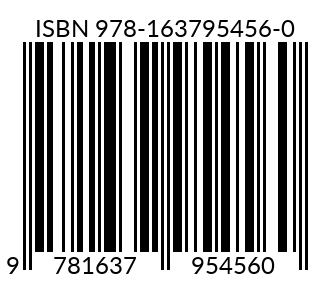
\includegraphics[keepaspectratio]{ISBN}}}}

\end{document}


